\batchmode
\documentclass[twoside]{article}
\RequirePackage{ifthen}


\hoffset-2.5cm
\voffset-2.5cm
\textwidth16cm
\textheight26cm
\oddsidemargin2.4cm
\evensidemargin2.4cm
\usepackage{graphicx}
 \usepackage{makeidx}
\usepackage{lscape}
\usepackage{amssymb}
\usepackage{amsbsy}
\makeindex%
\providecommand{\m}[1]{\overline{#1}}%
\providecommand{\M}[1]{\underline{#1}}%
\providecommand{\mbf}[1]{\mathbf #1}%
\providecommand{\V}[1]{ \stackrel{=}{\mathbf #1}}%
\providecommand{\B}[1]{#1}%
\providecommand{\prg}{\sl}%
\providecommand{\use}[1]{\vspace{0.5cm} Usage: {\sl { #1}} \vspace{0.5cm}}%
\providecommand{\bra}[1]{\langle #1|}%
\providecommand{\ket}[1]{|#1\rangle}%
\providecommand{\threej}[2]{\left( \begin{array}{ccc} #1 \\#2 \end{array} \right)}%
\providecommand{\sixj}[2]{\left\{ \begin{array}{ccc} #1 \\#2 \end{array} \right\}}%
\providecommand{\hili}[1]{{#1}}%
\providecommand{\hl}[1]{{#1}}%
\providecommand{\Bell}{\ensuremath{\boldsymbol\ell}}%
\providecommand{\bm}[1]{\boldsymbol #1}%
\providecommand{\Trace}[1]{\rm Tr \{ #1 \} } 




\usepackage[dvips]{color}


\pagecolor[gray]{.7}

\usepackage[latin1]{inputenc}



\makeatletter
\AtBeginDocument{\makeatletter
\input /run/media/rotter/MARTIN/mcphase/doc/manual.aux
\makeatother
}

\makeatletter
\count@=\the\catcode`\_ \catcode`\_=8 
\newenvironment{tex2html_wrap}{}{}%
\catcode`\<=12\catcode`\_=\count@
\newcommand{\providedcommand}[1]{\expandafter\providecommand\csname #1\endcsname}%
\newcommand{\renewedcommand}[1]{\expandafter\providecommand\csname #1\endcsname{}%
  \expandafter\renewcommand\csname #1\endcsname}%
\newcommand{\newedenvironment}[1]{\newenvironment{#1}{}{}\renewenvironment{#1}}%
\let\newedcommand\renewedcommand
\let\renewedenvironment\newedenvironment
\makeatother
\let\mathon=$
\let\mathoff=$
\ifx\AtBeginDocument\undefined \newcommand{\AtBeginDocument}[1]{}\fi
\newbox\sizebox
\setlength{\hoffset}{0pt}\setlength{\voffset}{0pt}
\addtolength{\textheight}{\footskip}\setlength{\footskip}{0pt}
\addtolength{\textheight}{\topmargin}\setlength{\topmargin}{0pt}
\addtolength{\textheight}{\headheight}\setlength{\headheight}{0pt}
\addtolength{\textheight}{\headsep}\setlength{\headsep}{0pt}
\setlength{\textwidth}{349pt}
\newwrite\lthtmlwrite
\makeatletter
\let\realnormalsize=\normalsize
\global\topskip=2sp
\def\preveqno{}\let\real@float=\@float \let\realend@float=\end@float
\def\@float{\let\@savefreelist\@freelist\real@float}
\def\liih@math{\ifmmode$\else\bad@math\fi}
\def\end@float{\realend@float\global\let\@freelist\@savefreelist}
\let\real@dbflt=\@dbflt \let\end@dblfloat=\end@float
\let\@largefloatcheck=\relax
\let\if@boxedmulticols=\iftrue
\def\@dbflt{\let\@savefreelist\@freelist\real@dbflt}
\def\adjustnormalsize{\def\normalsize{\mathsurround=0pt \realnormalsize
 \parindent=0pt\abovedisplayskip=0pt\belowdisplayskip=0pt}%
 \def\phantompar{\csname par\endcsname}\normalsize}%
\def\lthtmltypeout#1{{\let\protect\string \immediate\write\lthtmlwrite{#1}}}%
\newcommand\lthtmlhboxmathA{\adjustnormalsize\setbox\sizebox=\hbox\bgroup\kern.05em }%
\newcommand\lthtmlhboxmathB{\adjustnormalsize\setbox\sizebox=\hbox to\hsize\bgroup\hfill }%
\newcommand\lthtmlvboxmathA{\adjustnormalsize\setbox\sizebox=\vbox\bgroup %
 \let\ifinner=\iffalse \let\)\liih@math }%
\newcommand\lthtmlboxmathZ{\@next\next\@currlist{}{\def\next{\voidb@x}}%
 \expandafter\box\next\egroup}%
\newcommand\lthtmlmathtype[1]{\gdef\lthtmlmathenv{#1}}%
\newcommand\lthtmllogmath{\dimen0\ht\sizebox \advance\dimen0\dp\sizebox
  \ifdim\dimen0>.95\vsize
   \lthtmltypeout{%
*** image for \lthtmlmathenv\space is too tall at \the\dimen0, reducing to .95 vsize ***}%
   \ht\sizebox.95\vsize \dp\sizebox\z@ \fi
  \lthtmltypeout{l2hSize %
:\lthtmlmathenv:\the\ht\sizebox::\the\dp\sizebox::\the\wd\sizebox.\preveqno}}%
\newcommand\lthtmlfigureA[1]{\let\@savefreelist\@freelist
       \lthtmlmathtype{#1}\lthtmlvboxmathA}%
\newcommand\lthtmlpictureA{\bgroup\catcode`\_=8 \lthtmlpictureB}%
\newcommand\lthtmlpictureB[1]{\lthtmlmathtype{#1}\egroup
       \let\@savefreelist\@freelist \lthtmlhboxmathB}%
\newcommand\lthtmlpictureZ[1]{\hfill\lthtmlfigureZ}%
\newcommand\lthtmlfigureZ{\lthtmlboxmathZ\lthtmllogmath\copy\sizebox
       \global\let\@freelist\@savefreelist}%
\newcommand\lthtmldisplayA{\bgroup\catcode`\_=8 \lthtmldisplayAi}%
\newcommand\lthtmldisplayAi[1]{\lthtmlmathtype{#1}\egroup\lthtmlvboxmathA}%
\newcommand\lthtmldisplayB[1]{\edef\preveqno{(\theequation)}%
  \lthtmldisplayA{#1}\let\@eqnnum\relax}%
\newcommand\lthtmldisplayZ{\lthtmlboxmathZ\lthtmllogmath\lthtmlsetmath}%
\newcommand\lthtmlinlinemathA{\bgroup\catcode`\_=8 \lthtmlinlinemathB}
\newcommand\lthtmlinlinemathB[1]{\lthtmlmathtype{#1}\egroup\lthtmlhboxmathA
  \vrule height1.5ex width0pt }%
\newcommand\lthtmlinlineA{\bgroup\catcode`\_=8 \lthtmlinlineB}%
\newcommand\lthtmlinlineB[1]{\lthtmlmathtype{#1}\egroup\lthtmlhboxmathA}%
\newcommand\lthtmlinlineZ{\egroup\expandafter\ifdim\dp\sizebox>0pt %
  \expandafter\centerinlinemath\fi\lthtmllogmath\lthtmlsetinline}
\newcommand\lthtmlinlinemathZ{\egroup\expandafter\ifdim\dp\sizebox>0pt %
  \expandafter\centerinlinemath\fi\lthtmllogmath\lthtmlsetmath}
\newcommand\lthtmlindisplaymathZ{\egroup %
  \centerinlinemath\lthtmllogmath\lthtmlsetmath}
\def\lthtmlsetinline{\hbox{\vrule width.1em \vtop{\vbox{%
  \kern.1em\copy\sizebox}\ifdim\dp\sizebox>0pt\kern.1em\else\kern.3pt\fi
  \ifdim\hsize>\wd\sizebox \hrule depth1pt\fi}}}
\def\lthtmlsetmath{\hbox{\vrule width.1em\kern-.05em\vtop{\vbox{%
  \kern.1em\kern0.8 pt\hbox{\hglue.17em\copy\sizebox\hglue0.8 pt}}\kern.3pt%
  \ifdim\dp\sizebox>0pt\kern.1em\fi \kern0.8 pt%
  \ifdim\hsize>\wd\sizebox \hrule depth1pt\fi}}}
\def\centerinlinemath{%
  \dimen1=\ifdim\ht\sizebox<\dp\sizebox \dp\sizebox\else\ht\sizebox\fi
  \advance\dimen1by.5pt \vrule width0pt height\dimen1 depth\dimen1 
 \dp\sizebox=\dimen1\ht\sizebox=\dimen1\relax}

\def\lthtmlcheckvsize{\ifdim\ht\sizebox<\vsize 
  \ifdim\wd\sizebox<\hsize\expandafter\hfill\fi \expandafter\vfill
  \else\expandafter\vss\fi}%
\providecommand{\selectlanguage}[1]{}%
\makeatletter \tracingstats = 1 


\begin{document}
\pagestyle{empty}\thispagestyle{empty}\lthtmltypeout{}%
\lthtmltypeout{latex2htmlLength hsize=\the\hsize}\lthtmltypeout{}%
\lthtmltypeout{latex2htmlLength vsize=\the\vsize}\lthtmltypeout{}%
\lthtmltypeout{latex2htmlLength hoffset=\the\hoffset}\lthtmltypeout{}%
\lthtmltypeout{latex2htmlLength voffset=\the\voffset}\lthtmltypeout{}%
\lthtmltypeout{latex2htmlLength topmargin=\the\topmargin}\lthtmltypeout{}%
\lthtmltypeout{latex2htmlLength topskip=\the\topskip}\lthtmltypeout{}%
\lthtmltypeout{latex2htmlLength headheight=\the\headheight}\lthtmltypeout{}%
\lthtmltypeout{latex2htmlLength headsep=\the\headsep}\lthtmltypeout{}%
\lthtmltypeout{latex2htmlLength parskip=\the\parskip}\lthtmltypeout{}%
\lthtmltypeout{latex2htmlLength oddsidemargin=\the\oddsidemargin}\lthtmltypeout{}%
\makeatletter
\if@twoside\lthtmltypeout{latex2htmlLength evensidemargin=\the\evensidemargin}%
\else\lthtmltypeout{latex2htmlLength evensidemargin=\the\oddsidemargin}\fi%
\lthtmltypeout{}%
\makeatother
\setcounter{page}{1}
\onecolumn

% !!! IMAGES START HERE !!!

{\newpage\clearpage
\lthtmlinlinemathA{tex2html_wrap_inline21357}%
$_2$%
\lthtmlinlinemathZ
\lthtmlcheckvsize\clearpage}

{\newpage\clearpage
\lthtmlinlinemathA{tex2html_wrap_inline21359}%
$b$%
\lthtmlinlinemathZ
\lthtmlcheckvsize\clearpage}

{\newpage\clearpage
\lthtmlinlinemathA{tex2html_wrap_inline21371}%
$^{3+}$%
\lthtmlinlinemathZ
\lthtmlcheckvsize\clearpage}

{\newpage\clearpage
\lthtmlinlinemathA{tex2html_wrap_inline21389}%
$x$%
\lthtmlinlinemathZ
\lthtmlcheckvsize\clearpage}

{\newpage\clearpage
\lthtmlinlinemathA{tex2html_wrap_inline21391}%
$c$%
\lthtmlinlinemathZ
\lthtmlcheckvsize\clearpage}

{\newpage\clearpage
\lthtmlinlinemathA{tex2html_wrap_inline21393}%
$xyz$%
\lthtmlinlinemathZ
\lthtmlcheckvsize\clearpage}

{\newpage\clearpage
\lthtmlinlinemathA{tex2html_wrap_inline21395}%
$xyz||cab$%
\lthtmlinlinemathZ
\lthtmlcheckvsize\clearpage}

{\newpage\clearpage
\lthtmlinlinemathA{tex2html_wrap_inline21469}%
$_7$%
\lthtmlinlinemathZ
\lthtmlcheckvsize\clearpage}

{\newpage\clearpage
\lthtmlinlinemathA{tex2html_wrap_inline21471}%
$T=10$%
\lthtmlinlinemathZ
\lthtmlcheckvsize\clearpage}

{\newpage\clearpage
\lthtmlinlinemathA{tex2html_wrap_inline21537}%
$a$%
\lthtmlinlinemathZ
\lthtmlcheckvsize\clearpage}

{\newpage\clearpage
\lthtmlinlinemathA{tex2html_wrap_inline21545}%
$E_{el}$%
\lthtmlinlinemathZ
\lthtmlcheckvsize\clearpage}

{\newpage\clearpage
\lthtmlinlinemathA{tex2html_wrap_inline21548}%
$H_{mix}$%
\lthtmlinlinemathZ
\lthtmlcheckvsize\clearpage}

{\newpage\clearpage
\lthtmlinlinemathA{tex2html_wrap_inline21551}%
$H_{E}+H_{int}$%
\lthtmlinlinemathZ
\lthtmlcheckvsize\clearpage}

{\newpage\clearpage
\lthtmlinlinemathA{tex2html_wrap_inline21554}%
$\hat  I_a,\hat  I_b,\hat  I_c ...$%
\lthtmlinlinemathZ
\lthtmlcheckvsize\clearpage}

{\newpage\clearpage
\lthtmlinlinemathA{tex2html_wrap_inline21727}%
$T=$%
\lthtmlinlinemathZ
\lthtmlcheckvsize\clearpage}

{\newpage\clearpage
\lthtmlinlinemathA{tex2html_wrap_inline21729}%
$H=0$%
\lthtmlinlinemathZ
\lthtmlcheckvsize\clearpage}

{\newpage\clearpage
\lthtmlinlinemathA{tex2html_wrap_inline21776}%
$_4$%
\lthtmlinlinemathZ
\lthtmlcheckvsize\clearpage}

{\newpage\clearpage
\lthtmlinlinemathA{tex2html_wrap_inline21778}%
$_9$%
\lthtmlinlinemathZ
\lthtmlcheckvsize\clearpage}

{\newpage\clearpage
\lthtmlinlinemathA{tex2html_wrap_inline21780}%
$_3$%
\lthtmlinlinemathZ
\lthtmlcheckvsize\clearpage}

{\newpage\clearpage
\lthtmlinlinemathA{tex2html_wrap_inline21802}%
$m$%
\lthtmlinlinemathZ
\lthtmlcheckvsize\clearpage}

{\newpage\clearpage
\lthtmlinlinemathA{tex2html_wrap_inline21804}%
$\frac  {1}{2}$%
\lthtmlinlinemathZ
\lthtmlcheckvsize\clearpage}

{\newpage\clearpage
\lthtmlinlinemathA{tex2html_wrap_inline21806}%
$m\neq  0$%
\lthtmlinlinemathZ
\lthtmlcheckvsize\clearpage}

{\newpage\clearpage
\lthtmlinlinemathA{tex2html_wrap_inline21810}%
$m=0$%
\lthtmlinlinemathZ
\lthtmlcheckvsize\clearpage}

{\newpage\clearpage
\lthtmlinlinemathA{tex2html_wrap_inline21812}%
$\langle J || \theta _l || J \rangle $%
\lthtmlinlinemathZ
\lthtmlcheckvsize\clearpage}

{\newpage\clearpage
\lthtmlinlinemathA{tex2html_wrap_inline21814}%
$\langle L || \theta _l || L \rangle $%
\lthtmlinlinemathZ
\lthtmlcheckvsize\clearpage}

{\newpage\clearpage
\lthtmlinlinemathA{tex2html_wrap_inline21816}%
$L$%
\lthtmlinlinemathZ
\lthtmlcheckvsize\clearpage}

{\newpage\clearpage
\lthtmlinlinemathA{tex2html_wrap_inline21818}%
$d$%
\lthtmlinlinemathZ
\lthtmlcheckvsize\clearpage}

{\newpage\clearpage
\lthtmlinlinemathA{tex2html_wrap_inline21820}%
$\lambda _{lm}$%
\lthtmlinlinemathZ
\lthtmlcheckvsize\clearpage}

{\newpage\clearpage
\lthtmlinlinemathA{tex2html_wrap_inline21838}%
$\lambda _{lm} \equiv B_l^m/(\theta _lL_l^m)= A_{lm}\langle r^l \rangle / L_l^m$%
\lthtmlinlinemathZ
\lthtmlcheckvsize\clearpage}

{\newpage\clearpage
\lthtmlinlinemathA{tex2html_wrap_inline21842}%
$p_{lm}$%
\lthtmlinlinemathZ
\lthtmlcheckvsize\clearpage}

{\newpage\clearpage
\lthtmlinlinemathA{tex2html_wrap_inline21844}%
$\lambda _{l0} =\sqrt  {\frac  {4\pi }{2l+1}}|p_{l0}|$%
\lthtmlinlinemathZ
\lthtmlcheckvsize\clearpage}

{\newpage\clearpage
\lthtmlinlinemathA{tex2html_wrap_inline21846}%
$\lambda _{lm} =\sqrt  {\frac  {8\pi }{2l+1}}|p_{lm}|$%
\lthtmlinlinemathZ
\lthtmlcheckvsize\clearpage}

{\newpage\clearpage
\lthtmlinlinemathA{tex2html_wrap_inline21850}%
$B_m^l({\rm Newman})\equiv (-1)^m L_l^m$%
\lthtmlinlinemathZ
\lthtmlcheckvsize\clearpage}

{\newpage\clearpage
\lthtmlinlinemathA{tex2html_wrap_inline21862}%
$m>0$%
\lthtmlinlinemathZ
\lthtmlcheckvsize\clearpage}

{\newpage\clearpage
\lthtmlinlinemathA{tex2html_wrap_inline21864}%
$B_l^m$%
\lthtmlinlinemathZ
\lthtmlcheckvsize\clearpage}

{\newpage\clearpage
\lthtmlinlinemathA{tex2html_wrap_inline21901}%
$h$%
\lthtmlinlinemathZ
\lthtmlcheckvsize\clearpage}

{\newpage\clearpage
\lthtmlinlinemathA{tex2html_wrap_inline185}%
$\langle \mathbf S \rangle$%
\lthtmlinlinemathZ
\lthtmlcheckvsize\clearpage}

{\newpage\clearpage
\lthtmlinlinemathA{tex2html_wrap_inline187}%
$\langle \mathbf L \rangle$%
\lthtmlinlinemathZ
\lthtmlcheckvsize\clearpage}

{\newpage\clearpage
\lthtmlinlinemathA{tex2html_wrap_inline189}%
$H=D_{x4} S_x^4 +D_{y4} S_y^4 +D_{z4} S_x^4$%
\lthtmlinlinemathZ
\lthtmlcheckvsize\clearpage}

\stepcounter{section}
\stepcounter{section}
\stepcounter{section}
{\newpage\clearpage
\lthtmlpictureA{tex2html_wrap21955}%
\includegraphics[angle=0,width=0.7\columnwidth]{figsrc/mcphas_modules.eps}%
\lthtmlpictureZ
\lthtmlcheckvsize\clearpage}

{\newpage\clearpage
\lthtmlinlinemathA{tex2html_wrap_inline573}%
$T$%
\lthtmlinlinemathZ
\lthtmlcheckvsize\clearpage}

{\newpage\clearpage
\lthtmlinlinemathA{tex2html_wrap_inline575}%
$\mathbf H$%
\lthtmlinlinemathZ
\lthtmlcheckvsize\clearpage}

{\newpage\clearpage
\lthtmlpictureA{tex2html_wrap21972}%
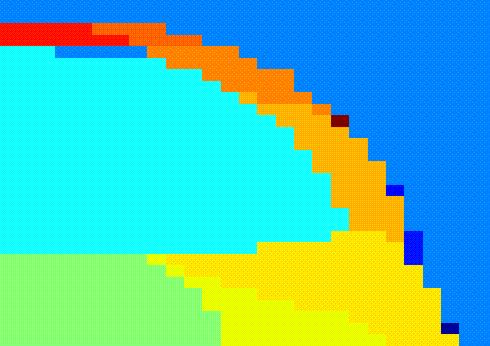
\includegraphics[angle=90,width=0.7\columnwidth]{figsrc/ndphased.eps}%
\lthtmlpictureZ
\lthtmlcheckvsize\clearpage}

\stepcounter{section}
\stepcounter{section}
{\newpage\clearpage
\lthtmldisplayA{displaymath423}%
\begin{displaymath}

 \hat \mathcal H=\sum_{n=1}^N \hat \mathcal H(n) -\frac{1}{2} \sum_{n,n',\alpha,\beta}
 {\mathcal J}_{\alpha\beta}(\mathbf R_{n'} - \mathbf R_n) \hat \mathcal I_{\alpha}^n \hat \mathcal I_{\beta}^{n'}.
 \end{displaymath}%
\lthtmldisplayZ
\lthtmlcheckvsize\clearpage}

{\newpage\clearpage
\lthtmlinlinemathA{tex2html_wrap_inline663}%
$\hat \mathcal H(n)$%
\lthtmlinlinemathZ
\lthtmlcheckvsize\clearpage}

{\newpage\clearpage
\lthtmlinlinemathA{tex2html_wrap_inline665}%
$n$%
\lthtmlinlinemathZ
\lthtmlcheckvsize\clearpage}

{\newpage\clearpage
\lthtmlinlinemathA{tex2html_wrap_inline667}%
$\hat \mathcal I_{\alpha}^n$%
\lthtmlinlinemathZ
\lthtmlcheckvsize\clearpage}

{\newpage\clearpage
\lthtmlinlinemathA{tex2html_wrap_inline669}%
$\alpha = 1,2,...,m$%
\lthtmlinlinemathZ
\lthtmlcheckvsize\clearpage}

{\newpage\clearpage
\lthtmlinlinemathA{tex2html_wrap_inline677}%
$[\hat \mathcal I_{\alpha}^n,\hat \mathcal I_{\alpha}^{n'}]=0$%
\lthtmlinlinemathZ
\lthtmlcheckvsize\clearpage}

{\newpage\clearpage
\lthtmlinlinemathA{tex2html_wrap_inline679}%
$[\hat \mathcal H(n),\hat \mathcal I_{\alpha}^{n'}]=0$%
\lthtmlinlinemathZ
\lthtmlcheckvsize\clearpage}

{\newpage\clearpage
\lthtmlinlinemathA{tex2html_wrap_inline681}%
$[\hat \mathcal H(n),\hat \mathcal H(n')]=0$%
\lthtmlinlinemathZ
\lthtmlcheckvsize\clearpage}

{\newpage\clearpage
\lthtmlinlinemathA{tex2html_wrap_inline683}%
$n \neq n'$%
\lthtmlinlinemathZ
\lthtmlcheckvsize\clearpage}

{\newpage\clearpage
\lthtmlinlinemathA{tex2html_wrap_inline685}%
$\alpha=1,2,3$%
\lthtmlinlinemathZ
\lthtmlcheckvsize\clearpage}

{\newpage\clearpage
\lthtmlinlinemathA{tex2html_wrap_inline687}%
$\hat \mathcal I_1 \leftrightarrow \hat S_x, \hat \mathcal I_2 %
\leftrightarrow \hat S_y, \hat \mathcal I_3 \leftrightarrow \hat S_z$%
\lthtmlinlinemathZ
\lthtmlcheckvsize\clearpage}

{\newpage\clearpage
\lthtmlinlinemathA{tex2html_wrap_inline689}%
${\mathcal J}_{\alpha\beta}(\mathbf R_n - \mathbf R_{n'})$%
\lthtmlinlinemathZ
\lthtmlcheckvsize\clearpage}

{\newpage\clearpage
\lthtmlinlinemathA{tex2html_wrap_inline691}%
$\alpha$%
\lthtmlinlinemathZ
\lthtmlcheckvsize\clearpage}

{\newpage\clearpage
\lthtmlinlinemathA{tex2html_wrap_inline695}%
$\hat \mathcal I^n_{\alpha}$%
\lthtmlinlinemathZ
\lthtmlcheckvsize\clearpage}

{\newpage\clearpage
\lthtmlinlinemathA{tex2html_wrap_inline697}%
$u^{n}$%
\lthtmlinlinemathZ
\lthtmlcheckvsize\clearpage}

{\newpage\clearpage
\lthtmlinlinemathA{tex2html_wrap_inline703}%
$n=(1,x),(1,y),(1,z),(2,x),(2,y),(2,z), ...$%
\lthtmlinlinemathZ
\lthtmlcheckvsize\clearpage}

\stepcounter{subsection}
{\newpage\clearpage
\lthtmlinlinemathA{tex2html_wrap_inline709}%
$\mathcal H$%
\lthtmlinlinemathZ
\lthtmlcheckvsize\clearpage}

{\newpage\clearpage
\lthtmldisplayA{displaymath453}%
\begin{displaymath}

 {\mathcal H}= \sum_{n,lm} B_l^m O_{lm}({\mathbf J}^n) 
             -\frac{1}{2}  \sum_{nn'} {\mathcal J}(nn') {\mathbf J}^n{\mathbf J}^{n'}
	     - \sum_{n} g_{Jn} \mu_B {\mathbf J}^n {\mathbf H} 
\end{displaymath}%
\lthtmldisplayZ
\lthtmlcheckvsize\clearpage}

{\newpage\clearpage
\lthtmlinlinemathA{tex2html_wrap_inline711}%
$O_l^m$%
\lthtmlinlinemathZ
\lthtmlcheckvsize\clearpage}

{\newpage\clearpage
\lthtmldisplayA{displaymath472}%
\begin{displaymath}

 {\mathcal H}_{JJ}=
             -\frac{1}{2}  \sum_{nn'} \sum_ {ll'} \sum_{mm'}
	     {\mathcal K}_{ll'}^{mm'}(nn') O_{lm}({\mathbf J}^n) O_{l'm'}({\mathbf J}^{n'})
\end{displaymath}%
\lthtmldisplayZ
\lthtmlcheckvsize\clearpage}

{\newpage\clearpage
\lthtmlinlinemathA{tex2html_wrap_inline715}%
${\mathcal J}(ij)$%
\lthtmlinlinemathZ
\lthtmlcheckvsize\clearpage}

{\newpage\clearpage
\lthtmlinlinemathA{tex2html_wrap_inline717}%
${\mathcal K}_{ll'}^{mm'}(ij)$%
\lthtmlinlinemathZ
\lthtmlcheckvsize\clearpage}

{\newpage\clearpage
\lthtmlinlinemathA{tex2html_wrap_inline719}%
$\epsilon$%
\lthtmlinlinemathZ
\lthtmlcheckvsize\clearpage}

\stepcounter{subsection}
{\newpage\clearpage
\lthtmlinlinemathA{tex2html_wrap_indisplay22238}%
$\displaystyle {\mathcal H}$%
\lthtmlindisplaymathZ
\lthtmlcheckvsize\clearpage}

{\newpage\clearpage
\lthtmlinlinemathA{tex2html_wrap_indisplay22239}%
$\textstyle =$%
\lthtmlindisplaymathZ
\lthtmlcheckvsize\clearpage}

{\newpage\clearpage
\lthtmlinlinemathA{tex2html_wrap_indisplay22240}%
$\displaystyle \sum_n \left \{ \sum_{i_n=1}^{\nu_n}
\left [ \frac{p_{i_n}^2}{2m_e}
-\frac{Z_n e^2}{4\pi\epsilon_0|\mathbf r_{i_n}-\mathbf R_n|}
+\zeta_n  \mathbf l^{i_n} \cdot \mathbf s^{i_n}
+ \sum_{lm} L_l^m(n) T_{lm}^n
\right ]
+ \sum_{i_n>j_n=1}^{\nu_n}\frac{e^2}{4\pi\epsilon_0|\mathbf r_{i_n}-\mathbf r_{j_n}|} \right \}$%
\lthtmlindisplaymathZ
\lthtmlcheckvsize\clearpage}

{\newpage\clearpage
\lthtmlinlinemathA{tex2html_wrap_indisplay22241}%
$\displaystyle - \sum_{n}  \mu_B (2\mathbf S^n+\mathbf L^n) {\mathbf H}$%
\lthtmlindisplaymathZ
\lthtmlcheckvsize\clearpage}

{\newpage\clearpage
\lthtmlinlinemathA{tex2html_wrap_indisplay22242}%
$\displaystyle -\frac{1}{2} \sum_{nn'} \left[
({\hat \mathbf L}^n,{\hat \mathbf S}^n )
\stackrel{=}{\mathcal J}(nn')
\left ( \begin{array}{c} {\hat \mathbf L}^{n'} \\
{\hat \mathbf S}^{n'} \end{array}
\right )
+ \sum_{kk'} \sum_{qq'}  \mathcal{K}_{kk'}^{qq'}(nn') \hat{T}_{kq}^n T_{k'q'}^{n'} \right]$%
\lthtmlindisplaymathZ
\lthtmlcheckvsize\clearpage}

{\newpage\clearpage
\lthtmlinlinemathA{tex2html_wrap_inline727}%
$\nu_n$%
\lthtmlinlinemathZ
\lthtmlcheckvsize\clearpage}

{\newpage\clearpage
\lthtmlinlinemathA{tex2html_wrap_inline729}%
$Z_n$%
\lthtmlinlinemathZ
\lthtmlcheckvsize\clearpage}

{\newpage\clearpage
\lthtmlinlinemathA{tex2html_wrap_inline731}%
$\mathbf R_n$%
\lthtmlinlinemathZ
\lthtmlcheckvsize\clearpage}

{\newpage\clearpage
\lthtmlinlinemathA{tex2html_wrap_inline735}%
$p$%
\lthtmlinlinemathZ
\lthtmlcheckvsize\clearpage}

{\newpage\clearpage
\lthtmlinlinemathA{tex2html_wrap_inline737}%
$m_e$%
\lthtmlinlinemathZ
\lthtmlcheckvsize\clearpage}

{\newpage\clearpage
\lthtmlinlinemathA{tex2html_wrap_inline739}%
$e$%
\lthtmlinlinemathZ
\lthtmlcheckvsize\clearpage}

{\newpage\clearpage
\lthtmlinlinemathA{tex2html_wrap_inline741}%
$\mathbf r$%
\lthtmlinlinemathZ
\lthtmlcheckvsize\clearpage}

{\newpage\clearpage
\lthtmlinlinemathA{tex2html_wrap_inline743}%
$\mathbf l$%
\lthtmlinlinemathZ
\lthtmlcheckvsize\clearpage}

{\newpage\clearpage
\lthtmlinlinemathA{tex2html_wrap_inline745}%
$\mathbf s$%
\lthtmlinlinemathZ
\lthtmlcheckvsize\clearpage}

{\newpage\clearpage
\lthtmlinlinemathA{tex2html_wrap_inline747}%
$\mathbf S_n$%
\lthtmlinlinemathZ
\lthtmlcheckvsize\clearpage}

{\newpage\clearpage
\lthtmlinlinemathA{tex2html_wrap_inline749}%
$\mathbf L_n$%
\lthtmlinlinemathZ
\lthtmlcheckvsize\clearpage}

{\newpage\clearpage
\lthtmlinlinemathA{tex2html_wrap_inline753}%
$L_l^m$%
\lthtmlinlinemathZ
\lthtmlcheckvsize\clearpage}

{\newpage\clearpage
\lthtmlinlinemathA{tex2html_wrap_inline755}%
$T_{lm}^n$%
\lthtmlinlinemathZ
\lthtmlcheckvsize\clearpage}

{\newpage\clearpage
\lthtmlinlinemathA{tex2html_wrap_inline757}%
$T_{l0}=\sqrt{4\pi/(2l+1)}\sum_iY_{l0}(\Omega_{i_n})$%
\lthtmlinlinemathZ
\lthtmlcheckvsize\clearpage}

{\newpage\clearpage
\lthtmlinlinemathA{tex2html_wrap_inline759}%
$T_{l,\pm|m|}=\sqrt{4\pi/(2l+1)}\sum_i \sqrt{\pm1}[Y_{l,-|m|}(\Omega_{i_n})\pm (-1)^m Y_{l,|m|}(\Omega_{i_n})]$%
\lthtmlinlinemathZ
\lthtmlcheckvsize\clearpage}

\stepcounter{section}
\stepcounter{subsection}
{\newpage\clearpage
\lthtmlpictureA{tex2html_wrap22266}%
\includegraphics[angle=0,width=0.7\columnwidth]{figsrc/crystalfieldplot.eps}%
\lthtmlpictureZ
\lthtmlcheckvsize\clearpage}

{\newpage\clearpage
\lthtmlpictureA{tex2html_wrap22274}%
\includegraphics[angle=0,width=0.7\columnwidth]{figsrc/chrgpla.eps}%
\lthtmlpictureZ
\lthtmlcheckvsize\clearpage}

{\newpage\clearpage
\lthtmlinlinemathA{tex2html_wrap_inline1223}%
$|JLSm_J \rangle$%
\lthtmlinlinemathZ
\lthtmlcheckvsize\clearpage}

{\newpage\clearpage
\lthtmldisplayA{displaymath968}%
\begin{displaymath}

 {\mathcal H}= \sum_{n,lm} B_{lm} O_{lm}({\mathbf J}^n) 
	     - \sum_{n} g_{Jn} \mu_B {\mathbf J}^n {\mathbf H} 
\end{displaymath}%
\lthtmldisplayZ
\lthtmlcheckvsize\clearpage}

{\newpage\clearpage
\lthtmldisplayA{displaymath988}%
\begin{displaymath}
  \sum_s D_x^2 (J_x^s)^2 + D_y^2 (J_y^s)^2 +D_z^2 (J_z^s)^2 
\end{displaymath}%
\lthtmldisplayZ
\lthtmlcheckvsize\clearpage}

\stepcounter{subsection}
{\newpage\clearpage
\lthtmldisplayA{displaymath1023}%
\begin{displaymath}
\sigma(i\rightarrow k)=\left(\frac{\hbar \gamma e^2}{mc^2}\right)^2
\frac{exp(-E_i/k_BT)}{\sum_j exp(-E_j/k_BT)} \frac{2}{3}\sum_{\alpha=x,y,z}
|\langle i|J_{\alpha}|k\rangle|^2
\end{displaymath}%
\lthtmldisplayZ
\lthtmlcheckvsize\clearpage}

{\newpage\clearpage
\lthtmlinlinemathA{tex2html_wrap_inline1231}%
$Q$%
\lthtmlinlinemathZ
\lthtmlcheckvsize\clearpage}

{\newpage\clearpage
\lthtmlinlinemathA{tex2html_wrap_inline1233}%
$k'/k$%
\lthtmlinlinemathZ
\lthtmlcheckvsize\clearpage}

{\newpage\clearpage
\lthtmlinlinemathA{tex2html_wrap_inline1235}%
$exp(-W(Q))$%
\lthtmlinlinemathZ
\lthtmlcheckvsize\clearpage}

{\newpage\clearpage
\lthtmlinlinemathA{tex2html_wrap_inline1237}%
$>$%
\lthtmlinlinemathZ
\lthtmlcheckvsize\clearpage}

{\newpage\clearpage
\lthtmlpictureA{tex2html_wrap22293}%
\includegraphics[angle=0,width=1.0\textwidth]{figsrc/10KCEFspectrum.eps}%
\lthtmlpictureZ
\lthtmlcheckvsize\clearpage}

{\newpage\clearpage
\lthtmlinlinemathA{tex2html_wrap_inline1243}%
$>>$%
\lthtmlinlinemathZ
\lthtmlcheckvsize\clearpage}

{\newpage\clearpage
\lthtmlpictureA{tex2html_wrap22309}%
\includegraphics[angle=0,width=0.7\columnwidth]{figsrc/moment.eps}%
\lthtmlpictureZ
\lthtmlcheckvsize\clearpage}

{\newpage\clearpage
\lthtmlpictureA{tex2html_wrap22315}%
\includegraphics[angle=0,width=0.7\columnwidth]{figsrc/cpall.eps}%
\lthtmlpictureZ
\lthtmlcheckvsize\clearpage}

{\newpage\clearpage
\lthtmlinlinemathA{tex2html_wrap_inline1259}%
$s$%
\lthtmlinlinemathZ
\lthtmlcheckvsize\clearpage}

{\newpage\clearpage
\lthtmlinlinemathA{tex2html_wrap_inline1261}%
$f$%
\lthtmlinlinemathZ
\lthtmlcheckvsize\clearpage}

{\newpage\clearpage
\lthtmldisplayA{displaymath1092}%
\begin{displaymath} 

\rho_{s-f}(T) = \frac{3\pi N m}{\hbar e^2 E_F} G^2(g-1)^2 \sum_{m_s,m_s',i,i'} 
      \langle m_s',i' | {\mathbf s \cdot J} | m_s, i \rangle^2 p_i f_{ii'}
\end{displaymath}%
\lthtmldisplayZ
\lthtmlcheckvsize\clearpage}

{\newpage\clearpage
\lthtmlinlinemathA{tex2html_wrap_inline1263}%
$G$%
\lthtmlinlinemathZ
\lthtmlcheckvsize\clearpage}

{\newpage\clearpage
\lthtmlinlinemathA{tex2html_wrap_inline1265}%
$p_i$%
\lthtmlinlinemathZ
\lthtmlcheckvsize\clearpage}

{\newpage\clearpage
\lthtmlinlinemathA{tex2html_wrap_inline1267}%
$e^{-\beta E_i}/Z$%
\lthtmlinlinemathZ
\lthtmlcheckvsize\clearpage}

{\newpage\clearpage
\lthtmlinlinemathA{tex2html_wrap_inline1269}%
$f_{ii'}$%
\lthtmlinlinemathZ
\lthtmlcheckvsize\clearpage}

{\newpage\clearpage
\lthtmlinlinemathA{tex2html_wrap_inline1271}%
$2/(1+e^{-\beta(E_i-E_{i'})})$%
\lthtmlinlinemathZ
\lthtmlcheckvsize\clearpage}

{\newpage\clearpage
\lthtmlinlinemathA{tex2html_wrap_inline1273}%
$|i\rangle$%
\lthtmlinlinemathZ
\lthtmlcheckvsize\clearpage}

{\newpage\clearpage
\lthtmlinlinemathA{tex2html_wrap_inline1275}%
${\mathbf s \cdot J}$%
\lthtmlinlinemathZ
\lthtmlcheckvsize\clearpage}

{\newpage\clearpage
\lthtmlinlinemathA{tex2html_wrap_inline1277}%
$\rho_0=(3\pi N m/\hbar e^2 E_F) G^2(g-1)^2$%
\lthtmlinlinemathZ
\lthtmlcheckvsize\clearpage}

{\newpage\clearpage
\lthtmlinlinemathA{tex2html_wrap_inline1279}%
$\rho_0 = 0.2$%
\lthtmlinlinemathZ
\lthtmlcheckvsize\clearpage}

{\newpage\clearpage
\lthtmlinlinemathA{tex2html_wrap_inline1281}%
$\Omega$%
\lthtmlinlinemathZ
\lthtmlcheckvsize\clearpage}

{\newpage\clearpage
\lthtmlinlinemathA{tex2html_wrap_inline1283}%
$2J+1$%
\lthtmlinlinemathZ
\lthtmlcheckvsize\clearpage}

{\newpage\clearpage
\lthtmlinlinemathA{tex2html_wrap_inline1285}%
$\rho_0 J(J+1)$%
\lthtmlinlinemathZ
\lthtmlcheckvsize\clearpage}

\stepcounter{subsection}
\stepcounter{subsubsection}
{\newpage\clearpage
\lthtmlinlinemathA{tex2html_wrap_inline1291}%
$\mathbf H^s$%
\lthtmlinlinemathZ
\lthtmlcheckvsize\clearpage}

{\newpage\clearpage
\lthtmldisplayA{displaymath1138}%
\begin{displaymath}

 {\hat \mathcal H}=  B_l^m \hat O_{lm}({\hat \mathbf J}) 
	     -  g_{J} \mu_B {\hat \mathbf J} \cdot {\mathbf H} - {\hat \mathbf J} \cdot { \mathbf H^s}
\end{displaymath}%
\lthtmldisplayZ
\lthtmlcheckvsize\clearpage}

{\newpage\clearpage
\lthtmlinlinemathA{tex2html_wrap_inline1293}%
$\langle \hat \mathbf J \rangle$%
\lthtmlinlinemathZ
\lthtmlcheckvsize\clearpage}

{\newpage\clearpage
\lthtmldisplayA{displaymath1149}%
\begin{displaymath}
\langle \hat \mathbf J \rangle =
\sum_{i=1}^{2J+1} p_{i} \langle i |\hat \mathbf J | i \rangle
\end{displaymath}%
\lthtmldisplayZ
\lthtmlcheckvsize\clearpage}

{\newpage\clearpage
\lthtmlinlinemathA{tex2html_wrap_indisplay22340}%
$\displaystyle p_{i}$%
\lthtmlindisplaymathZ
\lthtmlcheckvsize\clearpage}

{\newpage\clearpage
\lthtmlinlinemathA{tex2html_wrap_indisplay22342}%
$\displaystyle \frac{\exp(-\epsilon_{i}/kT)}{z}$%
\lthtmlindisplaymathZ
\lthtmlcheckvsize\clearpage}

{\newpage\clearpage
\lthtmlinlinemathA{tex2html_wrap_indisplay22343}%
$\displaystyle z$%
\lthtmlindisplaymathZ
\lthtmlcheckvsize\clearpage}

{\newpage\clearpage
\lthtmlinlinemathA{tex2html_wrap_indisplay22345}%
$\displaystyle \sum_{i=1}^{2J+1} \exp(-\epsilon_{i}/kT)$%
\lthtmlindisplaymathZ
\lthtmlcheckvsize\clearpage}

{\newpage\clearpage
\lthtmlinlinemathA{tex2html_wrap_inline1295}%
$z$%
\lthtmlinlinemathZ
\lthtmlcheckvsize\clearpage}

{\newpage\clearpage
\lthtmlinlinemathA{tex2html_wrap_inline1299}%
$\epsilon_{i}$%
\lthtmlinlinemathZ
\lthtmlcheckvsize\clearpage}

{\newpage\clearpage
\lthtmlinlinemathA{tex2html_wrap_inline1301}%
$\langle \mathbf J_i \rangle$%
\lthtmlinlinemathZ
\lthtmlcheckvsize\clearpage}

{\newpage\clearpage
\lthtmlinlinemathA{tex2html_wrap_inline1305}%
$u=\sum_{i=1}^{2J+1} p_{i} \epsilon_{i}$%
\lthtmlinlinemathZ
\lthtmlcheckvsize\clearpage}

\stepcounter{subsubsection}
{\newpage\clearpage
\lthtmlinlinemathA{tex2html_wrap_inline1309}%
$abc$%
\lthtmlinlinemathZ
\lthtmlcheckvsize\clearpage}

{\newpage\clearpage
\lthtmlinlinemathA{tex2html_wrap_inline1311}%
$\vec a||x$%
\lthtmlinlinemathZ
\lthtmlcheckvsize\clearpage}

{\newpage\clearpage
\lthtmlinlinemathA{tex2html_wrap_inline1313}%
$\vec b||y$%
\lthtmlinlinemathZ
\lthtmlcheckvsize\clearpage}

{\newpage\clearpage
\lthtmlinlinemathA{tex2html_wrap_inline1315}%
$\vec c||z$%
\lthtmlinlinemathZ
\lthtmlcheckvsize\clearpage}

{\newpage\clearpage
\lthtmlinlinemathA{tex2html_wrap_inline1317}%
$\vec a||y$%
\lthtmlinlinemathZ
\lthtmlcheckvsize\clearpage}

{\newpage\clearpage
\lthtmlinlinemathA{tex2html_wrap_inline1319}%
$\vec b||z$%
\lthtmlinlinemathZ
\lthtmlcheckvsize\clearpage}

{\newpage\clearpage
\lthtmlinlinemathA{tex2html_wrap_inline1321}%
$\vec c||x$%
\lthtmlinlinemathZ
\lthtmlcheckvsize\clearpage}

{\newpage\clearpage
\lthtmlinlinemathA{tex2html_wrap_inline1323}%
$y||\vec b$%
\lthtmlinlinemathZ
\lthtmlcheckvsize\clearpage}

{\newpage\clearpage
\lthtmlinlinemathA{tex2html_wrap_inline1325}%
$z||(\vec a \times \vec b)$%
\lthtmlinlinemathZ
\lthtmlcheckvsize\clearpage}

{\newpage\clearpage
\lthtmlinlinemathA{tex2html_wrap_inline1329}%
$y$%
\lthtmlinlinemathZ
\lthtmlcheckvsize\clearpage}

\stepcounter{section}
\stepcounter{subsection}
\stepcounter{subsubsection}
\stepcounter{subsubsection}
{\newpage\clearpage
\lthtmlinlinemathA{tex2html_wrap_inline1784}%
$Ha, Hb, Hc$%
\lthtmlinlinemathZ
\lthtmlcheckvsize\clearpage}

{\newpage\clearpage
\lthtmlinlinemathA{tex2html_wrap_inline1786}%
$\mathbf a,\mathbf b,\mathbf c$%
\lthtmlinlinemathZ
\lthtmlcheckvsize\clearpage}

{\newpage\clearpage
\lthtmlinlinemathA{tex2html_wrap_inline1788}%
$Hb||\mathbf b$%
\lthtmlinlinemathZ
\lthtmlcheckvsize\clearpage}

{\newpage\clearpage
\lthtmlinlinemathA{tex2html_wrap_inline1790}%
$Hc||(\mathbf a \times \mathbf b)$%
\lthtmlinlinemathZ
\lthtmlcheckvsize\clearpage}

{\newpage\clearpage
\lthtmlinlinemathA{tex2html_wrap_inline1792}%
$Ha$%
\lthtmlinlinemathZ
\lthtmlcheckvsize\clearpage}

{\newpage\clearpage
\lthtmlinlinemathA{tex2html_wrap_inline1794}%
$Hb$%
\lthtmlinlinemathZ
\lthtmlcheckvsize\clearpage}

{\newpage\clearpage
\lthtmlinlinemathA{tex2html_wrap_inline1796}%
$Hc$%
\lthtmlinlinemathZ
\lthtmlcheckvsize\clearpage}

{\newpage\clearpage
\lthtmlinlinemathA{tex2html_wrap_inline1798}%
$N_b$%
\lthtmlinlinemathZ
\lthtmlcheckvsize\clearpage}

{\newpage\clearpage
\lthtmldisplayA{displaymath1679}%
\begin{displaymath}
 {\hat \mathcal H}=\sum_{s=1}^{N_b} \hat H^{MF}(s) + E_{corr}
\end{displaymath}%
\lthtmldisplayZ
\lthtmlcheckvsize\clearpage}

{\newpage\clearpage
\lthtmldisplayA{displaymath1686}%
\begin{displaymath}
\hat H^{MF}(s)=  \hat H(s) 
	     - \sum_{\alpha=1}^{\rm nofcomponents} H_{\alpha}^s \hat I_{\alpha}^s
\end{displaymath}%
\lthtmldisplayZ
\lthtmlcheckvsize\clearpage}

{\newpage\clearpage
\lthtmlinlinemathA{tex2html_wrap_inline1800}%
${\rm nofcomponents}=3$%
\lthtmlinlinemathZ
\lthtmlcheckvsize\clearpage}

{\newpage\clearpage
\lthtmlinlinemathA{tex2html_wrap_inline1802}%
$\hat I_{\alpha}=\hat J_{\alpha}$%
\lthtmlinlinemathZ
\lthtmlcheckvsize\clearpage}

{\newpage\clearpage
\lthtmlinlinemathA{tex2html_wrap_inline1804}%
$\mathbf M=g_{J} \mu_B \langle \hat \mathbf J \rangle$%
\lthtmlinlinemathZ
\lthtmlcheckvsize\clearpage}

{\newpage\clearpage
\lthtmldisplayA{displaymath1698}%
\begin{displaymath}
\hat H^{MF}_{\rm so1ion}(s)=  \underbrace{ B_l^m \hat O_{lm}({\hat \mathbf J}^s) 
	     - g_{Js} \mu_B {\hat \mathbf J}^s \cdot {\mathbf H} }_{\hat H(s) }-   {\hat \mathbf I}^s \cdot {\mathbf H}^s 
\end{displaymath}%
\lthtmldisplayZ
\lthtmlcheckvsize\clearpage}

{\newpage\clearpage
\lthtmlinlinemathA{tex2html_wrap_inline1806}%
${\mathbf H}^s$%
\lthtmlinlinemathZ
\lthtmlcheckvsize\clearpage}

{\newpage\clearpage
\lthtmlinlinemathA{tex2html_wrap_inline1810}%
${\mathbf H}$%
\lthtmlinlinemathZ
\lthtmlcheckvsize\clearpage}

{\newpage\clearpage
\lthtmldisplayA{displaymath1712}%
\begin{displaymath}
E_{corr}=\frac{1}{2}\sum_{s=1}^{N_b}\sum_{\alpha=1}^{\rm nofcomponents}  \langle {\hat I}^s_{\alpha}
 \rangle {H}^s_{\alpha} 
\end{displaymath}%
\lthtmldisplayZ
\lthtmlcheckvsize\clearpage}

{\newpage\clearpage
\lthtmldisplayA{displaymath1726}%
\begin{displaymath}

H^s_{\alpha}=\sum_{\mathbf G'}\sum_{s'=1}^{N_b}\sum_{\beta=1}^{\rm nofcomponents} {\mathcal J}_{\alpha\beta}
(\mathbf r_s-(\mathbf G'+\mathbf r_{s'})) \langle \hat I^{s'}_{\beta} \rangle
\end{displaymath}%
\lthtmldisplayZ
\lthtmlcheckvsize\clearpage}

{\newpage\clearpage
\lthtmlinlinemathA{tex2html_wrap_inline1816}%
$\langle {\hat\mathbf I}^s \rangle$%
\lthtmlinlinemathZ
\lthtmlcheckvsize\clearpage}

{\newpage\clearpage
\lthtmlinlinemathA{tex2html_wrap_indisplay22401}%
$\displaystyle f$%
\lthtmlindisplaymathZ
\lthtmlcheckvsize\clearpage}

{\newpage\clearpage
\lthtmlinlinemathA{tex2html_wrap_indisplay22403}%
$\displaystyle -kT\frac{1}{N_b}\sum_s \ln(z_s) + \frac{E_{corr}}{N_B}$%
\lthtmlindisplaymathZ
\lthtmlcheckvsize\clearpage}

{\newpage\clearpage
\lthtmlinlinemathA{tex2html_wrap_indisplay22404}%
$\displaystyle z_s$%
\lthtmlindisplaymathZ
\lthtmlcheckvsize\clearpage}

{\newpage\clearpage
\lthtmlinlinemathA{tex2html_wrap_indisplay22406}%
$\displaystyle \sum_i \exp(-\epsilon^s_i/kT) \, {\rm\dots  partition \, sum \, of \, the \, site} \, s$%
\lthtmlindisplaymathZ
\lthtmlcheckvsize\clearpage}

{\newpage\clearpage
\lthtmlinlinemathA{tex2html_wrap_indisplay22407}%
$\displaystyle \epsilon_i^s \, {\rm\dots  \, eigenvalues \, of \, }\hat H^{MF}(s)$%
\lthtmlindisplaymathZ
\lthtmlcheckvsize\clearpage}

{\newpage\clearpage
\lthtmlpictureA{tex2html_wrap22411}%
\includegraphics[angle=0,width=0.9\columnwidth]{figsrc/fecalc.eps}%
\lthtmlpictureZ
\lthtmlcheckvsize\clearpage}

\stepcounter{subsubsection}
\stepcounter{subsubsection}
{\newpage\clearpage
\lthtmlinlinemathA{tex2html_wrap_inline2034}%
$g_J$%
\lthtmlinlinemathZ
\lthtmlcheckvsize\clearpage}

{\newpage\clearpage
\lthtmlinlinemathA{tex2html_wrap_inline2036}%
$d_a$%
\lthtmlinlinemathZ
\lthtmlcheckvsize\clearpage}

{\newpage\clearpage
\lthtmlinlinemathA{tex2html_wrap_inline2038}%
$d_b$%
\lthtmlinlinemathZ
\lthtmlcheckvsize\clearpage}

{\newpage\clearpage
\lthtmlinlinemathA{tex2html_wrap_inline2040}%
$d_c$%
\lthtmlinlinemathZ
\lthtmlcheckvsize\clearpage}

{\newpage\clearpage
\lthtmlinlinemathA{tex2html_wrap_inline2042}%
$^{st}$%
\lthtmlinlinemathZ
\lthtmlcheckvsize\clearpage}

{\newpage\clearpage
\lthtmlinlinemathA{tex2html_wrap_inline2044}%
$\vec a$%
\lthtmlinlinemathZ
\lthtmlcheckvsize\clearpage}

{\newpage\clearpage
\lthtmlinlinemathA{tex2html_wrap_inline2046}%
$\vec b$%
\lthtmlinlinemathZ
\lthtmlcheckvsize\clearpage}

{\newpage\clearpage
\lthtmlinlinemathA{tex2html_wrap_inline2048}%
$\vec c$%
\lthtmlinlinemathZ
\lthtmlcheckvsize\clearpage}

{\newpage\clearpage
\lthtmlinlinemathA{tex2html_wrap_inline2056}%
$\vec r_1$%
\lthtmlinlinemathZ
\lthtmlcheckvsize\clearpage}

{\newpage\clearpage
\lthtmlinlinemathA{tex2html_wrap_inline2058}%
$\vec r_2$%
\lthtmlinlinemathZ
\lthtmlcheckvsize\clearpage}

{\newpage\clearpage
\lthtmlinlinemathA{tex2html_wrap_inline2060}%
$\vec r_3$%
\lthtmlinlinemathZ
\lthtmlcheckvsize\clearpage}

{\newpage\clearpage
\lthtmlinlinemathA{tex2html_wrap_inline2062}%
$ d_a \vec a + d_b \vec b + d_c \vec c = d_1 \vec r_1 + d_2 \vec r_2 + d_3 \vec r_3$%
\lthtmlinlinemathZ
\lthtmlcheckvsize\clearpage}

{\newpage\clearpage
\lthtmlinlinemathA{tex2html_wrap_inline2064}%
$\stackrel{=}{\mathcal J}$%
\lthtmlinlinemathZ
\lthtmlcheckvsize\clearpage}

{\newpage\clearpage
\lthtmlinlinemathA{tex2html_wrap_inline2066}%
$Ja, Jb, Jc, Jaa, Jbb, Jcc, Jab ...$%
\lthtmlinlinemathZ
\lthtmlcheckvsize\clearpage}

{\newpage\clearpage
\lthtmlinlinemathA{tex2html_wrap_inline2068}%
$\vec a,\vec b,\vec c$%
\lthtmlinlinemathZ
\lthtmlcheckvsize\clearpage}

{\newpage\clearpage
\lthtmlinlinemathA{tex2html_wrap_inline2070}%
$Jb||\vec b$%
\lthtmlinlinemathZ
\lthtmlcheckvsize\clearpage}

{\newpage\clearpage
\lthtmlinlinemathA{tex2html_wrap_inline2072}%
$Jc||(\vec a \times \vec b)$%
\lthtmlinlinemathZ
\lthtmlcheckvsize\clearpage}

{\newpage\clearpage
\lthtmlinlinemathA{tex2html_wrap_inline2074}%
$Ja$%
\lthtmlinlinemathZ
\lthtmlcheckvsize\clearpage}

{\newpage\clearpage
\lthtmlinlinemathA{tex2html_wrap_inline2076}%
$Jb$%
\lthtmlinlinemathZ
\lthtmlcheckvsize\clearpage}

{\newpage\clearpage
\lthtmlinlinemathA{tex2html_wrap_inline2078}%
$Jc$%
\lthtmlinlinemathZ
\lthtmlcheckvsize\clearpage}

{\newpage\clearpage
\lthtmlinlinemathA{tex2html_wrap_inline2086}%
$-d_a$%
\lthtmlinlinemathZ
\lthtmlcheckvsize\clearpage}

{\newpage\clearpage
\lthtmlinlinemathA{tex2html_wrap_inline2088}%
$-d_b$%
\lthtmlinlinemathZ
\lthtmlcheckvsize\clearpage}

{\newpage\clearpage
\lthtmlinlinemathA{tex2html_wrap_inline2090}%
$-d_c$%
\lthtmlinlinemathZ
\lthtmlcheckvsize\clearpage}

\stepcounter{subsubsection}
\stepcounter{subsubsection}
\stepcounter{subsubsection}
{\newpage\clearpage
\lthtmlinlinemathA{tex2html_wrap_inline2110}%
$||$%
\lthtmlinlinemathZ
\lthtmlcheckvsize\clearpage}

\stepcounter{subsubsection}
{\newpage\clearpage
\lthtmlinlinemathA{tex2html_wrap_inline2259}%
${\mathbf r}_i$%
\lthtmlinlinemathZ
\lthtmlcheckvsize\clearpage}

{\newpage\clearpage
\lthtmlinlinemathA{tex2html_wrap_inline2261}%
$3n$%
\lthtmlinlinemathZ
\lthtmlcheckvsize\clearpage}

{\newpage\clearpage
\lthtmlinlinemathA{tex2html_wrap_inline2263}%
$n=$%
\lthtmlinlinemathZ
\lthtmlcheckvsize\clearpage}

{\newpage\clearpage
\lthtmlinlinemathA{tex2html_wrap_inline2265}%
$<J>$%
\lthtmlinlinemathZ
\lthtmlcheckvsize\clearpage}

\stepcounter{subsubsection}
{\newpage\clearpage
\lthtmlinlinemathA{tex2html_wrap_inline2435}%
$mb||\vec b$%
\lthtmlinlinemathZ
\lthtmlcheckvsize\clearpage}

{\newpage\clearpage
\lthtmlinlinemathA{tex2html_wrap_inline2437}%
$mc||(\vec a \times \vec b)$%
\lthtmlinlinemathZ
\lthtmlcheckvsize\clearpage}

{\newpage\clearpage
\lthtmlinlinemathA{tex2html_wrap_inline2439}%
$ma$%
\lthtmlinlinemathZ
\lthtmlcheckvsize\clearpage}

{\newpage\clearpage
\lthtmlinlinemathA{tex2html_wrap_inline2441}%
$mb$%
\lthtmlinlinemathZ
\lthtmlcheckvsize\clearpage}

{\newpage\clearpage
\lthtmlinlinemathA{tex2html_wrap_inline2443}%
$mc$%
\lthtmlinlinemathZ
\lthtmlcheckvsize\clearpage}

\stepcounter{subsubsection}
\stepcounter{subsubsection}
{\newpage\clearpage
\lthtmlinlinemathA{tex2html_wrap_inline2451}%
${\rm sta}=\sum_{\rm data points i} ({\mathbf m}_i^{calc}-{\mathbf m}_i^{meas})^2$%
\lthtmlinlinemathZ
\lthtmlcheckvsize\clearpage}

\stepcounter{subsection}
{\newpage\clearpage
\lthtmlinlinemathA{tex2html_wrap_inline2453}%
$H-T$%
\lthtmlinlinemathZ
\lthtmlcheckvsize\clearpage}

\stepcounter{subsection}
{\newpage\clearpage
\lthtmlinlinemathA{tex2html_wrap_inline2455}%
$T-H$%
\lthtmlinlinemathZ
\lthtmlcheckvsize\clearpage}

{\newpage\clearpage
\lthtmlpictureA{tex2html_wrap22495}%
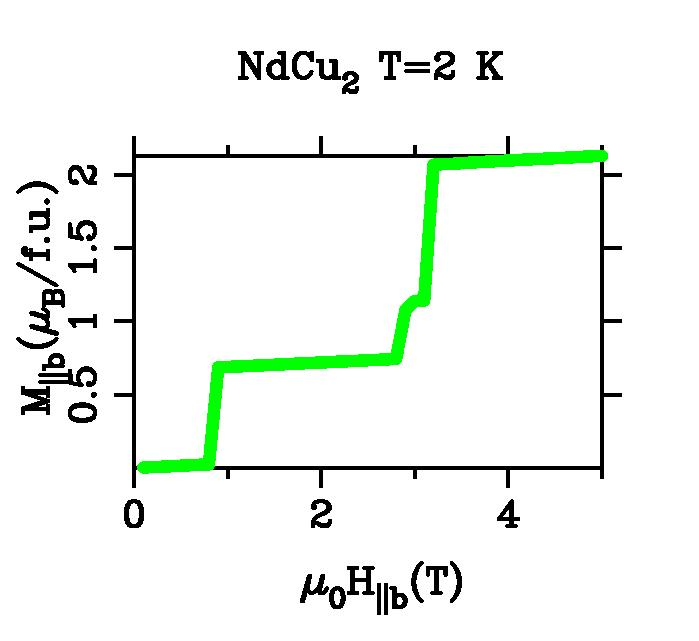
\includegraphics[angle=0, width=0.3\textwidth]{figsrc/magnetization_ndcu2.eps}%
\lthtmlpictureZ
\lthtmlcheckvsize\clearpage}

{\newpage\clearpage
\lthtmlpictureA{tex2html_wrap22503}%
\includegraphics[angle=0, width=0.8\textwidth]{figsrc/magnetostriction_ndcu2.eps}%
\lthtmlpictureZ
\lthtmlcheckvsize\clearpage}

\stepcounter{subsection}
{\newpage\clearpage
\lthtmlinlinemathA{tex2html_wrap_inline2463}%
$\vec a^*,\vec b^*,\vec c^*$%
\lthtmlinlinemathZ
\lthtmlcheckvsize\clearpage}

{\newpage\clearpage
\lthtmlinlinemathA{tex2html_wrap_inline2471}%
$\langle \hat I_{\alpha} \rangle$%
\lthtmlinlinemathZ
\lthtmlcheckvsize\clearpage}

{\newpage\clearpage
\lthtmlinlinemathA{tex2html_wrap_inline2473}%
$\alpha=1,\dots,{\rm nofcomponents}$%
\lthtmlinlinemathZ
\lthtmlcheckvsize\clearpage}

{\newpage\clearpage
\lthtmlinlinemathA{tex2html_wrap_inline2475}%
$\hat I_1=\hat J_x,\hat I_2=\hat J_y,\hat I_3=\hat J_z,\hat I_4=\hat O_2^{-2},\hat I_5=\hat O_2^{-1}, \dots$%
\lthtmlinlinemathZ
\lthtmlcheckvsize\clearpage}

{\newpage\clearpage
\lthtmlinlinemathA{tex2html_wrap_inline2479}%
$H_{xc}(i)$%
\lthtmlinlinemathZ
\lthtmlcheckvsize\clearpage}

{\newpage\clearpage
\lthtmlinlinemathA{tex2html_wrap_inline2483}%
$u$%
\lthtmlinlinemathZ
\lthtmlcheckvsize\clearpage}

{\newpage\clearpage
\lthtmldisplayA{displaymath2382}%
\begin{displaymath}
u=f+Ts=f-T\partial f/\partial T=\frac{1}{N_b}\sum_{s,i} \epsilon^s_i \frac{e^{-\epsilon^s_i/kT}}{z^s}+\frac{E_{corr}}{N_b}
\end{displaymath}%
\lthtmldisplayZ
\lthtmlcheckvsize\clearpage}

{\newpage\clearpage
\lthtmlinlinemathA{tex2html_wrap_inline2487}%
$c_V=\partial u/\partial T$%
\lthtmlinlinemathZ
\lthtmlcheckvsize\clearpage}

{\newpage\clearpage
\lthtmlinlinemathA{tex2html_wrap_inline2493}%
$ma,mb,mc$%
\lthtmlinlinemathZ
\lthtmlcheckvsize\clearpage}

{\newpage\clearpage
\lthtmlinlinemathA{tex2html_wrap_inline2495}%
$Hb||\vec b$%
\lthtmlinlinemathZ
\lthtmlcheckvsize\clearpage}

{\newpage\clearpage
\lthtmlinlinemathA{tex2html_wrap_inline2497}%
$Hc||(\vec a \times \vec b)$%
\lthtmlinlinemathZ
\lthtmlcheckvsize\clearpage}

{\newpage\clearpage
\lthtmlinlinemathA{tex2html_wrap_inline2505}%
$k$%
\lthtmlinlinemathZ
\lthtmlcheckvsize\clearpage}

{\newpage\clearpage
\lthtmldisplayA{displaymath2394}%
\begin{displaymath}
	        \frac{1}{N_b}\sum_{s=1}^{N_b} <{\hat \mathbf I}^s> \otimes  <{\hat \mathbf I}^{s+k}>
	       \end{displaymath}%
\lthtmldisplayZ
\lthtmlcheckvsize\clearpage}

{\newpage\clearpage
\lthtmlinlinemathA{tex2html_wrap_inline2511}%
$<\hat I_{\alpha}>$%
\lthtmlinlinemathZ
\lthtmlcheckvsize\clearpage}

{\newpage\clearpage
\lthtmlinlinemathA{tex2html_wrap_inline2551}%
$h,k,l$%
\lthtmlinlinemathZ
\lthtmlcheckvsize\clearpage}

\stepcounter{section}
{\newpage\clearpage
\lthtmlinlinemathA{tex2html_wrap_inline3238}%
$a,b,c$%
\lthtmlinlinemathZ
\lthtmlcheckvsize\clearpage}

{\newpage\clearpage
\lthtmlinlinemathA{tex2html_wrap_inline3240}%
$\alpha,\beta,\gamma$%
\lthtmlinlinemathZ
\lthtmlcheckvsize\clearpage}

{\newpage\clearpage
\lthtmlinlinemathA{tex2html_wrap_inline3242}%
$\Theta$%
\lthtmlinlinemathZ
\lthtmlcheckvsize\clearpage}

\stepcounter{subsection}
{\newpage\clearpage
\lthtmlinlinemathA{tex2html_wrap_inline3244}%
$2\Theta$%
\lthtmlinlinemathZ
\lthtmlcheckvsize\clearpage}

{\newpage\clearpage
\lthtmlpictureA{tex2html_wrap22608}%
\includegraphics[angle=0,width=1.1\textwidth]{figsrc/patternAF1.eps}%
\lthtmlpictureZ
\lthtmlcheckvsize\clearpage}

\stepcounter{subsection}
{\newpage\clearpage
\lthtmlinlinemathA{tex2html_wrap_inline3248}%
$R_{\rm p}=100
\frac{\sum_{hkl} |I_{calc}(hkl)-I_{exp}(hkl)|}{\sum_{hkl}|I_{\rm 
exp}(hkl)|}$%
\lthtmlinlinemathZ
\lthtmlcheckvsize\clearpage}

{\newpage\clearpage
\lthtmlinlinemathA{tex2html_wrap_inline3250}%
$\chi^2=\sum_{hkl}\frac{ (I_{calc}(hkl)-I_{exp}(hkl))^2}{n(\Delta I_{\rm 
experror}(hkl))^2}$%
\lthtmlinlinemathZ
\lthtmlcheckvsize\clearpage}

\stepcounter{subsection}
{\newpage\clearpage
\lthtmlinlinemathA{tex2html_wrap_indisplay22616}%
$\displaystyle f_{nE1}^{RXMS}=$%
\lthtmlindisplaymathZ
\lthtmlcheckvsize\clearpage}

{\newpage\clearpage
\lthtmlinlinemathA{tex2html_wrap_indisplay22617}%
$\displaystyle =\left (
\begin{array}{cc}
\sigma \rightarrow \sigma & \pi \rightarrow \sigma \\
\sigma \rightarrow \pi & \pi \rightarrow \pi
\end{array}
\right) = F^{(0)}
\left ( \begin{array}{cc}
1 & 0 \\
0 & \cos2\Theta
\end{array} \right )
-iF^{(1)}$%
\lthtmlindisplaymathZ
\lthtmlcheckvsize\clearpage}

{\newpage\clearpage
\lthtmlinlinemathA{tex2html_wrap_indisplay22618}%
$\displaystyle \times
\left ( \begin{array}{cc}
0 & z_1 \cos \Theta + z_3 \sin \Theta \\
z_3 \sin \Theta - z_1 \cos \Theta & -z_2 \sin 2\Theta
\end{array} \right ) + F^{(2)}$%
\lthtmlindisplaymathZ
\lthtmlcheckvsize\clearpage}

{\newpage\clearpage
\lthtmlinlinemathA{tex2html_wrap_indisplay22619}%
$\displaystyle \times
\left ( \begin{array}{cc}
z_2^2 & -z_2(z_1 \sin \Theta - z_3 \cos \Theta) \\
+z_2(z_1 \sin \Theta + z_3 \cos \Theta) & -\cos^2 \Theta (z_1^2 \tan^2 \Theta + z_3^2)
\end{array} \right )$%
\lthtmlindisplaymathZ
\lthtmlcheckvsize\clearpage}

{\newpage\clearpage
\lthtmlinlinemathA{tex2html_wrap_inline3260}%
$z_1, z_2$%
\lthtmlinlinemathZ
\lthtmlcheckvsize\clearpage}

{\newpage\clearpage
\lthtmlinlinemathA{tex2html_wrap_inline3262}%
$z_3$%
\lthtmlinlinemathZ
\lthtmlcheckvsize\clearpage}

{\newpage\clearpage
\lthtmlinlinemathA{tex2html_wrap_inline3264}%
$[\mathbf u_1,\mathbf u_2,\mathbf u_3]$%
\lthtmlinlinemathZ
\lthtmlcheckvsize\clearpage}

{\newpage\clearpage
\lthtmlinlinemathA{tex2html_wrap_inline3266}%
$\mathbf k$%
\lthtmlinlinemathZ
\lthtmlcheckvsize\clearpage}

{\newpage\clearpage
\lthtmlinlinemathA{tex2html_wrap_inline3268}%
$\mathbf k'$%
\lthtmlinlinemathZ
\lthtmlcheckvsize\clearpage}

{\newpage\clearpage
\lthtmlinlinemathA{tex2html_wrap_inline3270}%
$\mathbf u_1$%
\lthtmlinlinemathZ
\lthtmlcheckvsize\clearpage}

{\newpage\clearpage
\lthtmlinlinemathA{tex2html_wrap_inline3274}%
$\mathbf u_3$%
\lthtmlinlinemathZ
\lthtmlcheckvsize\clearpage}

{\newpage\clearpage
\lthtmlinlinemathA{tex2html_wrap_inline3276}%
$\mathbf Q=\mathbf k-\mathbf k'$%
\lthtmlinlinemathZ
\lthtmlcheckvsize\clearpage}

{\newpage\clearpage
\lthtmlinlinemathA{tex2html_wrap_inline3278}%
$F^{(1)}$%
\lthtmlinlinemathZ
\lthtmlcheckvsize\clearpage}

{\newpage\clearpage
\lthtmlinlinemathA{tex2html_wrap_inline3280}%
$F^(2)$%
\lthtmlinlinemathZ
\lthtmlcheckvsize\clearpage}

{\newpage\clearpage
\lthtmlinlinemathA{tex2html_wrap_inline3282}%
$z_i$%
\lthtmlinlinemathZ
\lthtmlcheckvsize\clearpage}

{\newpage\clearpage
\lthtmlinlinemathA{tex2html_wrap_inline3284}%
$\mu_a,\mu_b$%
\lthtmlinlinemathZ
\lthtmlcheckvsize\clearpage}

{\newpage\clearpage
\lthtmlinlinemathA{tex2html_wrap_inline3286}%
$\mu_c$%
\lthtmlinlinemathZ
\lthtmlcheckvsize\clearpage}

{\newpage\clearpage
\lthtmlinlinemathA{tex2html_wrap_inline3288}%
$\mathbf a$%
\lthtmlinlinemathZ
\lthtmlcheckvsize\clearpage}

{\newpage\clearpage
\lthtmlinlinemathA{tex2html_wrap_inline3290}%
$\mathbf b$%
\lthtmlinlinemathZ
\lthtmlcheckvsize\clearpage}

{\newpage\clearpage
\lthtmlinlinemathA{tex2html_wrap_inline3292}%
$\mathbf c$%
\lthtmlinlinemathZ
\lthtmlcheckvsize\clearpage}

{\newpage\clearpage
\lthtmlinlinemathA{tex2html_wrap_indisplay22640}%
$\displaystyle z_1$%
\lthtmlindisplaymathZ
\lthtmlcheckvsize\clearpage}

{\newpage\clearpage
\lthtmlinlinemathA{tex2html_wrap_indisplay22642}%
$\displaystyle \mu_a \sin \alpha_1 \cos(\Psi+\delta_1)+\mu_b \sin \alpha_2 \cos(\Psi +\delta_2)$%
\lthtmlindisplaymathZ
\lthtmlcheckvsize\clearpage}

{\newpage\clearpage
\lthtmlinlinemathA{tex2html_wrap_indisplay22643}%
$\displaystyle +\mu_c \sin \alpha_3 \cos (\Psi +\delta_3),$%
\lthtmlindisplaymathZ
\lthtmlcheckvsize\clearpage}

{\newpage\clearpage
\lthtmlinlinemathA{tex2html_wrap_indisplay22644}%
$\displaystyle z_2$%
\lthtmlindisplaymathZ
\lthtmlcheckvsize\clearpage}

{\newpage\clearpage
\lthtmlinlinemathA{tex2html_wrap_indisplay22646}%
$\displaystyle \mu_a \sin \alpha_1 \sin (\Psi +\delta_1)+\mu_b \sin \alpha_2 \sin (\Psi+\delta_2)$%
\lthtmlindisplaymathZ
\lthtmlcheckvsize\clearpage}

{\newpage\clearpage
\lthtmlinlinemathA{tex2html_wrap_indisplay22647}%
$\displaystyle +\mu_c \sin \alpha_3 \sin (\Psi +\delta_3)$%
\lthtmlindisplaymathZ
\lthtmlcheckvsize\clearpage}

{\newpage\clearpage
\lthtmlinlinemathA{tex2html_wrap_indisplay22648}%
$\displaystyle z_3$%
\lthtmlindisplaymathZ
\lthtmlcheckvsize\clearpage}

{\newpage\clearpage
\lthtmlinlinemathA{tex2html_wrap_indisplay22650}%
$\displaystyle \mu_a \cos \alpha_1 + \mu_b \cos \alpha_2 + \mu_c \cos \alpha_3$%
\lthtmlindisplaymathZ
\lthtmlcheckvsize\clearpage}

{\newpage\clearpage
\lthtmlinlinemathA{tex2html_wrap_inline3294}%
$\alpha_i=\angle(\mathbf a_i \cdot \mathbf u_3)_{\Psi=0}$%
\lthtmlinlinemathZ
\lthtmlcheckvsize\clearpage}

{\newpage\clearpage
\lthtmlinlinemathA{tex2html_wrap_inline3296}%
$\delta_i=\angle(\mathbf a_i^{\perp}\cdot %
\mathbf u_1)_{\Psi=0}$%
\lthtmlinlinemathZ
\lthtmlcheckvsize\clearpage}

{\newpage\clearpage
\lthtmlinlinemathA{tex2html_wrap_inline3298}%
$\mathbf a_{1,2,3}=\mathbf a,\mathbf b,\mathbf c$%
\lthtmlinlinemathZ
\lthtmlcheckvsize\clearpage}

{\newpage\clearpage
\lthtmlinlinemathA{tex2html_wrap_inline3300}%
$\mathbf a_i^{\perp}$%
\lthtmlinlinemathZ
\lthtmlcheckvsize\clearpage}

{\newpage\clearpage
\lthtmlinlinemathA{tex2html_wrap_inline3302}%
$\mathbf a_i$%
\lthtmlinlinemathZ
\lthtmlcheckvsize\clearpage}

{\newpage\clearpage
\lthtmlinlinemathA{tex2html_wrap_inline3304}%
$\mathbf Q$%
\lthtmlinlinemathZ
\lthtmlcheckvsize\clearpage}

{\newpage\clearpage
\lthtmlinlinemathA{tex2html_wrap_inline3306}%
$\Psi=0$%
\lthtmlinlinemathZ
\lthtmlcheckvsize\clearpage}

\stepcounter{subsection}
{\newpage\clearpage
\lthtmldisplayA{displaymath2925}%
\begin{displaymath}

\frac{d^2\sigma}{d\Omega dE'}=N\frac{k'}{k}\left( \frac{\hbar \gamma e^2}{m_e c^2}  \right)^2
\sum_{\alpha\beta=x,y,z}(\delta_{\alpha\beta}-\hat \mathbf Q_{\alpha} \hat \mathbf Q_{\beta}) 
S^{\alpha \beta}_{\rm mag}(\mathbf Q,\omega)+
N\frac{k'}{k}S_{\rm nuc}(\mathbf Q,\omega)
\end{displaymath}%
\lthtmldisplayZ
\lthtmlcheckvsize\clearpage}

{\newpage\clearpage
\lthtmlinlinemathA{tex2html_wrap_inline3310}%
$\frac{d^2\sigma}{d\Omega dE'}$%
\lthtmlinlinemathZ
\lthtmlcheckvsize\clearpage}

{\newpage\clearpage
\lthtmlinlinemathA{tex2html_wrap_inline3312}%
$N$%
\lthtmlinlinemathZ
\lthtmlcheckvsize\clearpage}

{\newpage\clearpage
\lthtmlinlinemathA{tex2html_wrap_inline3316}%
$k'$%
\lthtmlinlinemathZ
\lthtmlcheckvsize\clearpage}

{\newpage\clearpage
\lthtmlinlinemathA{tex2html_wrap_inline3318}%
$\gamma=\frac{g_n}{2\hbar}$%
\lthtmlinlinemathZ
\lthtmlcheckvsize\clearpage}

{\newpage\clearpage
\lthtmlinlinemathA{tex2html_wrap_inline3320}%
$e^2/m_ec^2=2.82$%
\lthtmlinlinemathZ
\lthtmlcheckvsize\clearpage}

{\newpage\clearpage
\lthtmlinlinemathA{tex2html_wrap_inline3324}%
$\hbar \omega=E-E'=\frac{(\hbar\mathbf k)^2}{2m_n}-\frac{(\hbar\mathbf k')^2}{2m_n}$%
\lthtmlinlinemathZ
\lthtmlcheckvsize\clearpage}

{\newpage\clearpage
\lthtmlinlinemathA{tex2html_wrap_inline3326}%
$S$%
\lthtmlinlinemathZ
\lthtmlcheckvsize\clearpage}

{\newpage\clearpage
\lthtmlinlinemathA{tex2html_wrap_indisplay22671}%
$\displaystyle S_{\rm nuc}$%
\lthtmlindisplaymathZ
\lthtmlcheckvsize\clearpage}

{\newpage\clearpage
\lthtmlinlinemathA{tex2html_wrap_indisplay22673}%
$\displaystyle S_{\rm nuc}^{\rm el}+S_{\rm nuc}^{\rm inel}$%
\lthtmlindisplaymathZ
\lthtmlcheckvsize\clearpage}

{\newpage\clearpage
\lthtmlinlinemathA{tex2html_wrap_indisplay22674}%
$\displaystyle S_{\rm mag}$%
\lthtmlindisplaymathZ
\lthtmlcheckvsize\clearpage}

{\newpage\clearpage
\lthtmlinlinemathA{tex2html_wrap_indisplay22676}%
$\displaystyle S_{\rm mag}^{\rm el}+S_{\rm mag}^{\rm inel}$%
\lthtmlindisplaymathZ
\lthtmlcheckvsize\clearpage}

{\newpage\clearpage
\lthtmldisplayA{displaymath2964}%
\begin{displaymath}
S_{\rm nuc}^{\rm el}=S_{\rm nuc}^{\rm el,inc}+S_{\rm nuc}^{\rm el,coh}
\end{displaymath}%
\lthtmldisplayZ
\lthtmlcheckvsize\clearpage}

{\newpage\clearpage
\lthtmlinlinemathA{tex2html_wrap_indisplay22679}%
$\displaystyle S_{\rm nuc}^{\rm el,coh}$%
\lthtmlindisplaymathZ
\lthtmlcheckvsize\clearpage}

{\newpage\clearpage
\lthtmlinlinemathA{tex2html_wrap_indisplay22681}%
$\displaystyle \delta(\hbar \omega)
\left ( \frac{(2\pi)^3}{v_0}\sum_{\mathbf \tau } \delta(\mathbf Q-\mathbf \tau ) \right )
\frac{1}{N_B} \left ( \sum_{dd'} \bar b_d^* \bar b_{d'} e^{-i\mathbf Q(\mathbf B_d-\mathbf B_{d'})} e^{-W_d-W_{d'}} %
\right )$%
\lthtmlindisplaymathZ
\lthtmlcheckvsize\clearpage}

{\newpage\clearpage
\lthtmlinlinemathA{tex2html_wrap_indisplay22683}%
$\displaystyle \delta(\hbar \omega)
\left ( \frac{(2\pi)^3}{v_0}\sum_{\mathbf \tau } \delta(\mathbf Q-\mathbf \tau ) \right )
\frac{1}{N_B}|NSF|^2$%
\lthtmlindisplaymathZ
\lthtmlcheckvsize\clearpage}

{\newpage\clearpage
\lthtmlinlinemathA{tex2html_wrap_inline3328}%
$N_B$%
\lthtmlinlinemathZ
\lthtmlcheckvsize\clearpage}

{\newpage\clearpage
\lthtmlinlinemathA{tex2html_wrap_inline3330}%
$\mathbf \tau $%
\lthtmlinlinemathZ
\lthtmlcheckvsize\clearpage}

{\newpage\clearpage
\lthtmlinlinemathA{tex2html_wrap_inline3332}%
$d=1,\dots,N_B$%
\lthtmlinlinemathZ
\lthtmlcheckvsize\clearpage}

{\newpage\clearpage
\lthtmlinlinemathA{tex2html_wrap_inline3334}%
$v_0$%
\lthtmlinlinemathZ
\lthtmlcheckvsize\clearpage}

{\newpage\clearpage
\lthtmlinlinemathA{tex2html_wrap_inline3336}%
$\bar b_d$%
\lthtmlinlinemathZ
\lthtmlcheckvsize\clearpage}

{\newpage\clearpage
\lthtmlinlinemathA{tex2html_wrap_inline3338}%
$\mathbf B_d$%
\lthtmlinlinemathZ
\lthtmlcheckvsize\clearpage}

{\newpage\clearpage
\lthtmlinlinemathA{tex2html_wrap_inline3340}%
$W_d$%
\lthtmlinlinemathZ
\lthtmlcheckvsize\clearpage}

{\newpage\clearpage
\lthtmlinlinemathA{tex2html_wrap_inline3344}%
$W_d= \langle (\mathbf Q.\mathbf u_d)^2 \rangle/2=\langle u_{\rm iso}^2 \rangle Q^2/2=B_{\rm iso}Q^2/16\pi^2=
B_{\rm iso} sin^2 \Theta / \lambda^2$%
\lthtmlinlinemathZ
\lthtmlcheckvsize\clearpage}

{\newpage\clearpage
\lthtmlinlinemathA{tex2html_wrap_indisplay22694}%
$\displaystyle \sum_{\alpha\beta}(\delta_{\alpha\beta}-\hat \mathbf Q_{\alpha} \hat \mathbf Q_{\beta})S_{\rm mag}^{\rm %
el,\alpha\beta}$%
\lthtmlindisplaymathZ
\lthtmlcheckvsize\clearpage}

{\newpage\clearpage
\lthtmlinlinemathA{tex2html_wrap_indisplay22696}%
$\displaystyle \delta(\hbar \omega)
\left ( \frac{(2\pi)^3}{v_0}\sum_{\mathbf \tau } \delta(\mathbf Q-\mathbf \tau ) \right )
\frac{1}{N_B} \left ( \sum_{dd',\alpha\beta}(\delta_{\alpha\beta}-\hat \mathbf Q_{\alpha} \hat \mathbf Q_{\beta})
\frac{1}{2\mu_B}F_d(Q) M_{d\alpha} \right.$%
\lthtmlindisplaymathZ
\lthtmlcheckvsize\clearpage}

{\newpage\clearpage
\lthtmlinlinemathA{tex2html_wrap_indisplay22697}%
$\displaystyle \left.  \frac{1}{2\mu_B}F_{d'}(Q) M_{d'\beta}
e^{-i\mathbf Q(\mathbf B_d-\mathbf B_{d'})} e^{-W_d-W_{d'}} \right )$%
\lthtmlindisplaymathZ
\lthtmlcheckvsize\clearpage}

{\newpage\clearpage
\lthtmlinlinemathA{tex2html_wrap_indisplay22699}%
$\displaystyle \delta(\hbar \omega)\left ( \frac{(2\pi)^3}{v_0}\sum_{\mathbf \tau } \delta(\mathbf Q-\mathbf \tau ) \right )
\frac{1}{N_B} |\vec{\rm MSF}|^2$%
\lthtmlindisplaymathZ
\lthtmlcheckvsize\clearpage}

{\newpage\clearpage
\lthtmlinlinemathA{tex2html_wrap_inline3346}%
$F_d(Q) M_{d\alpha}$%
\lthtmlinlinemathZ
\lthtmlcheckvsize\clearpage}

{\newpage\clearpage
\lthtmlinlinemathA{tex2html_wrap_inline3348}%
$g_J\neq0$%
\lthtmlinlinemathZ
\lthtmlcheckvsize\clearpage}

{\newpage\clearpage
\lthtmlinlinemathA{tex2html_wrap_inline3350}%
$F_d(Q) M_{d\alpha}=g_J \mu_B\langle J_{d\alpha} \rangle_{T,H}\left [\langle j_0(Q) \rangle + \frac{2-g_J}{g_J}\langle j_2(Q) \rangle \right ]$%
\lthtmlinlinemathZ
\lthtmlcheckvsize\clearpage}

{\newpage\clearpage
\lthtmlinlinemathA{tex2html_wrap_inline3352}%
$g_J=0$%
\lthtmlinlinemathZ
\lthtmlcheckvsize\clearpage}

{\newpage\clearpage
\lthtmlinlinemathA{tex2html_wrap_inline3354}%
$\langle Ma \rangle, \langle Mb \rangle, \langle Mc \rangle$%
\lthtmlinlinemathZ
\lthtmlcheckvsize\clearpage}

{\newpage\clearpage
\lthtmlinlinemathA{tex2html_wrap_inline3356}%
$F_d(Q) M_{d\alpha}= \langle M_{d\alpha} \rangle_{T,H}\left [\langle j_0(Q) \rangle  \right ]$%
\lthtmlinlinemathZ
\lthtmlcheckvsize\clearpage}

{\newpage\clearpage
\lthtmlinlinemathA{tex2html_wrap_inline3362}%
$\langle Sa \rangle, \langle La \rangle, \langle Sb \rangle, \langle Lb \rangle, \langle Sc \rangle, \langle Lc \rangle$%
\lthtmlinlinemathZ
\lthtmlcheckvsize\clearpage}

{\newpage\clearpage
\lthtmlinlinemathA{tex2html_wrap_inline3364}%
$F_d(Q) M_{d\alpha}= \mu_B\langle 2 S_{d\alpha} \rangle_{T,H}\langle j_0(Q) \rangle +\mu_B \langle L_{d\alpha} \rangle_{T,H}\left [ \langle j_0(Q) \rangle + \langle j_2(Q) \rangle \right ] $%
\lthtmlinlinemathZ
\lthtmlcheckvsize\clearpage}

{\newpage\clearpage
\lthtmlinlinemathA{tex2html_wrap_inline3368}%
$F_d(Q)$%
\lthtmlinlinemathZ
\lthtmlcheckvsize\clearpage}

{\newpage\clearpage
\lthtmlinlinemathA{tex2html_wrap_inline3370}%
$\langle S_{d\alpha} \rangle_{T,H}$%
\lthtmlinlinemathZ
\lthtmlcheckvsize\clearpage}

{\newpage\clearpage
\lthtmlinlinemathA{tex2html_wrap_inline3372}%
$\langle L_{d\alpha} \rangle_{T,H}$%
\lthtmlinlinemathZ
\lthtmlcheckvsize\clearpage}

{\newpage\clearpage
\lthtmlinlinemathA{tex2html_wrap_inline3374}%
$\langle J_{d\alpha} \rangle_{T,H}$%
\lthtmlinlinemathZ
\lthtmlcheckvsize\clearpage}

{\newpage\clearpage
\lthtmlinlinemathA{tex2html_wrap_inline3380}%
$\mathbf Q=h\mathbf a^*+k \mathbf b^*+l \mathbf c^*$%
\lthtmlinlinemathZ
\lthtmlcheckvsize\clearpage}

{\newpage\clearpage
\lthtmldisplayA{displaymath3052}%
\begin{displaymath}
\sin(\Theta)=\lambda \frac{|\mathbf Q|}{4\pi}
\end{displaymath}%
\lthtmldisplayZ
\lthtmlcheckvsize\clearpage}

{\newpage\clearpage
\lthtmldisplayA{displaymath3056}%
\begin{displaymath}
I^{nuc}_{hkl}=|\frac{\rm NSF}{N_B}|^2 \exp(-\frac{{\rm OTF}\times Q^2}{8\pi^2}) \times {\rm LF} 
\end{displaymath}%
\lthtmldisplayZ
\lthtmlcheckvsize\clearpage}

{\newpage\clearpage
\lthtmldisplayA{displaymath3065}%
\begin{displaymath}
I^{mag}_{hkl}=\frac{3.65}{4\pi}|\frac{\vec{\rm MSF}}{N_B}|^2  \exp(-\frac{{\rm OTF}\times Q^2}{8\pi^2}) \times {\rm %
LF} 
\end{displaymath}%
\lthtmldisplayZ
\lthtmlcheckvsize\clearpage}

{\newpage\clearpage
\lthtmlinlinemathA{tex2html_wrap_indisplay22722}%
$\displaystyle {\rm OTF}$%
\lthtmlindisplaymathZ
\lthtmlcheckvsize\clearpage}

{\newpage\clearpage
\lthtmlinlinemathA{tex2html_wrap_indisplay22724}%
$\displaystyle {\rm ... Overall Temperature Factor (}B_{\rm iso}),{\rm OTF}.Q^2/(8\pi^2) =\langle (\mathbf Q.\mathbf %
u)^2 \rangle = \langle u^2 \rangle Q^2$%
\lthtmlindisplaymathZ
\lthtmlcheckvsize\clearpage}

{\newpage\clearpage
\lthtmlinlinemathA{tex2html_wrap_indisplay22725}%
$\displaystyle {\rm LF}$%
\lthtmlindisplaymathZ
\lthtmlcheckvsize\clearpage}

{\newpage\clearpage
\lthtmlinlinemathA{tex2html_wrap_indisplay22727}%
$\displaystyle {\rm ... Lorentzfactor}$%
\lthtmlindisplaymathZ
\lthtmlcheckvsize\clearpage}

{\newpage\clearpage
\lthtmlinlinemathA{tex2html_wrap_indisplay22729}%
$\displaystyle \sin^{-2}(2\Theta){\rm ... powder flat sample}$%
\lthtmlindisplaymathZ
\lthtmlcheckvsize\clearpage}

{\newpage\clearpage
\lthtmlinlinemathA{tex2html_wrap_indisplay22731}%
$\displaystyle \sin^{-1}(2\Theta)\sin^{-1}(\Theta){\rm ... powder cylindrical sample}$%
\lthtmlindisplaymathZ
\lthtmlcheckvsize\clearpage}

{\newpage\clearpage
\lthtmlinlinemathA{tex2html_wrap_indisplay22733}%
$\displaystyle \sin^{-1}(2\Theta){\rm ...single crystal sample}$%
\lthtmlindisplaymathZ
\lthtmlcheckvsize\clearpage}

{\newpage\clearpage
\lthtmlinlinemathA{tex2html_wrap_indisplay22735}%
$\displaystyle d^3 {\rm ... TOF powder cylindrical sample log scaled d pattern}$%
\lthtmlindisplaymathZ
\lthtmlcheckvsize\clearpage}

{\newpage\clearpage
\lthtmlinlinemathA{tex2html_wrap_indisplay22737}%
$\displaystyle d^4 {\rm ... TOF powder cylindrical sample linear scaled d pattern}$%
\lthtmlindisplaymathZ
\lthtmlcheckvsize\clearpage}

{\newpage\clearpage
\lthtmlinlinemathA{tex2html_wrap_indisplay22738}%
$\displaystyle {\rm NSF}$%
\lthtmlindisplaymathZ
\lthtmlcheckvsize\clearpage}

{\newpage\clearpage
\lthtmlinlinemathA{tex2html_wrap_indisplay22740}%
$\displaystyle {\rm ... nuclear structure factor}$%
\lthtmlindisplaymathZ
\lthtmlcheckvsize\clearpage}

{\newpage\clearpage
\lthtmlinlinemathA{tex2html_wrap_indisplay22742}%
$\displaystyle \sum_{d} \bar b_d e^{i\mathbf Q \mathbf B_d} e^{-W_d}$%
\lthtmlindisplaymathZ
\lthtmlcheckvsize\clearpage}

{\newpage\clearpage
\lthtmlinlinemathA{tex2html_wrap_indisplay22743}%
$\displaystyle \vec{\rm MSF}$%
\lthtmlindisplaymathZ
\lthtmlcheckvsize\clearpage}

{\newpage\clearpage
\lthtmlinlinemathA{tex2html_wrap_indisplay22745}%
$\displaystyle {\rm ... magnetic structure factor}$%
\lthtmlindisplaymathZ
\lthtmlcheckvsize\clearpage}

{\newpage\clearpage
\lthtmlinlinemathA{tex2html_wrap_indisplay22747}%
$\displaystyle \sum_{d}\frac{1}{2\mu_B}F_d(Q) \vec M^{\perp}_{d} e^{i\mathbf Q\mathbf B_d} e^{-W_d}$%
\lthtmlindisplaymathZ
\lthtmlcheckvsize\clearpage}

\stepcounter{subsection}
{\newpage\clearpage
\lthtmlinlinemathA{tex2html_wrap_inline3382}%
$\langle j_4(Q) \rangle$%
\lthtmlinlinemathZ
\lthtmlcheckvsize\clearpage}

{\newpage\clearpage
\lthtmlinlinemathA{tex2html_wrap_inline3384}%
$\langle j_6(Q) \rangle$%
\lthtmlinlinemathZ
\lthtmlcheckvsize\clearpage}

{\newpage\clearpage
\lthtmlinlinemathA{tex2html_wrap_inline3386}%
$\langle j_0(Q) \rangle$%
\lthtmlinlinemathZ
\lthtmlcheckvsize\clearpage}

{\newpage\clearpage
\lthtmlinlinemathA{tex2html_wrap_inline3388}%
$\langle j_2(Q) \rangle$%
\lthtmlinlinemathZ
\lthtmlcheckvsize\clearpage}

{\newpage\clearpage
\lthtmlinlinemathA{tex2html_wrap_inline3390}%
$Z(K)$%
\lthtmlinlinemathZ
\lthtmlcheckvsize\clearpage}

{\newpage\clearpage
\lthtmlinlinemathA{tex2html_wrap_inline3396}%
$\langle M_{d\alpha} \rangle_{T,H}$%
\lthtmlinlinemathZ
\lthtmlcheckvsize\clearpage}

{\newpage\clearpage
\lthtmlinlinemathA{tex2html_wrap_inline3398}%
$|MSF|^2$%
\lthtmlinlinemathZ
\lthtmlcheckvsize\clearpage}

{\newpage\clearpage
\lthtmlinlinemathA{tex2html_wrap_indisplay22759}%
$\displaystyle |\vec{\rm MSF}|^2$%
\lthtmlindisplaymathZ
\lthtmlcheckvsize\clearpage}

{\newpage\clearpage
\lthtmlinlinemathA{tex2html_wrap_indisplay22761}%
$\displaystyle \left ( \sum_{dd',\alpha\beta}(\delta_{\alpha\beta}-\hat \mathbf Q_{\alpha} \hat \mathbf Q_{\beta})
\langle \hat \mathcal Q^{d \dag }_{\alpha} \rangle_{T,H}
\langle \hat \mathcal Q^{d'}_{\beta} \rangle_{T,H}
e^{-i\mathbf Q(\mathbf B_d-\mathbf B_{d'})} e^{-W_d-W_{d'}} \right )$%
\lthtmlindisplaymathZ
\lthtmlcheckvsize\clearpage}

{\newpage\clearpage
\lthtmlinlinemathA{tex2html_wrap_inline3400}%
$\langle \dots \rangle_{T,H}$%
\lthtmlinlinemathZ
\lthtmlcheckvsize\clearpage}

{\newpage\clearpage
\lthtmlinlinemathA{tex2html_wrap_inline3402}%
$\hat \mathcal Q_{\alpha}$%
\lthtmlinlinemathZ
\lthtmlcheckvsize\clearpage}

{\newpage\clearpage
\lthtmlinlinemathA{tex2html_wrap_inline3406}%
$\hat \mathcal Q=\frac{1}{2\mu_B}\hat M(\mathbf Q)$%
\lthtmlinlinemathZ
\lthtmlcheckvsize\clearpage}

{\newpage\clearpage
\lthtmlinlinemathA{tex2html_wrap_inline3410}%
$|SLJM \rangle $%
\lthtmlinlinemathZ
\lthtmlcheckvsize\clearpage}

{\newpage\clearpage
\lthtmlinlinemathA{tex2html_wrap_inline3412}%
$M=-J,-J+1,\dots J$%
\lthtmlinlinemathZ
\lthtmlcheckvsize\clearpage}

{\newpage\clearpage
\lthtmlinlinemathA{tex2html_wrap_inline3414}%
$i$%
\lthtmlinlinemathZ
\lthtmlcheckvsize\clearpage}

{\newpage\clearpage
\lthtmlinlinemathA{tex2html_wrap_indisplay22771}%
$\displaystyle \langle SLJM|\hat \mathcal Q_x |SLJM' \rangle$%
\lthtmlindisplaymathZ
\lthtmlcheckvsize\clearpage}

{\newpage\clearpage
\lthtmlinlinemathA{tex2html_wrap_indisplay22773}%
$\displaystyle \frac{1}{2} \sum_{K',Q'} f(K') P(K',Q') \times$%
\lthtmlindisplaymathZ
\lthtmlcheckvsize\clearpage}

{\newpage\clearpage
\lthtmlinlinemathA{tex2html_wrap_indisplay22774}%
$\displaystyle \times               [Y_{K'-1,Q'+1}(\hat \mathbf Q)\sqrt{(K'-Q')(K'-Q'-1)}-
Y_{K'-1,Q'-1}(\hat \mathbf Q)\sqrt{(K'+Q')(K'+Q'-1)}]$%
\lthtmlindisplaymathZ
\lthtmlcheckvsize\clearpage}

{\newpage\clearpage
\lthtmlinlinemathA{tex2html_wrap_indisplay22775}%
$\displaystyle \langle SLJM|\hat \mathcal Q_y |SLJM' \rangle$%
\lthtmlindisplaymathZ
\lthtmlcheckvsize\clearpage}

{\newpage\clearpage
\lthtmlinlinemathA{tex2html_wrap_indisplay22777}%
$\displaystyle \frac{-i}{2} \sum_{K',Q'} f(K') P(K',Q') \times$%
\lthtmlindisplaymathZ
\lthtmlcheckvsize\clearpage}

{\newpage\clearpage
\lthtmlinlinemathA{tex2html_wrap_indisplay22778}%
$\displaystyle \times               [Y_{K'-1,Q'+1}(\hat \mathbf Q)\sqrt{(K'-Q')(K'-Q'-1)}+
Y_{K'-1,Q'-1}(\hat \mathbf Q)\sqrt{(K'+Q')(K'+Q'-1)}]$%
\lthtmlindisplaymathZ
\lthtmlcheckvsize\clearpage}

{\newpage\clearpage
\lthtmlinlinemathA{tex2html_wrap_indisplay22779}%
$\displaystyle \langle SLJM|\hat \mathcal Q_z |SLJM' \rangle$%
\lthtmlindisplaymathZ
\lthtmlcheckvsize\clearpage}

{\newpage\clearpage
\lthtmlinlinemathA{tex2html_wrap_indisplay22781}%
$\displaystyle \sum_{K',Q'} f(K') P(K',Q')
[Y_{K'-1,Q'}(\hat \mathbf Q)\sqrt{(K'-Q')(K'+Q')}]$%
\lthtmlindisplaymathZ
\lthtmlcheckvsize\clearpage}

{\newpage\clearpage
\lthtmlinlinemathA{tex2html_wrap_indisplay22783}%
$\displaystyle Z(K')$%
\lthtmlindisplaymathZ
\lthtmlcheckvsize\clearpage}

{\newpage\clearpage
\lthtmlinlinemathA{tex2html_wrap_indisplay22785}%
$\displaystyle c_{K'-1} \langle j_{K'-1}(Q) \rangle+c_{K'+1} \langle  j_{K'+1}(Q) \rangle$%
\lthtmlindisplaymathZ
\lthtmlcheckvsize\clearpage}

{\newpage\clearpage
\lthtmlinlinemathA{tex2html_wrap_indisplay22786}%
$\displaystyle f(K')$%
\lthtmlindisplaymathZ
\lthtmlcheckvsize\clearpage}

{\newpage\clearpage
\lthtmlinlinemathA{tex2html_wrap_indisplay22788}%
$\displaystyle \sqrt{4\pi}Z(K')/K'$%
\lthtmlindisplaymathZ
\lthtmlcheckvsize\clearpage}

{\newpage\clearpage
\lthtmlinlinemathA{tex2html_wrap_indisplay22789}%
$\displaystyle P(K',Q')$%
\lthtmlindisplaymathZ
\lthtmlcheckvsize\clearpage}

{\newpage\clearpage
\lthtmlinlinemathA{tex2html_wrap_indisplay22791}%
$\displaystyle (-1)^{J-M'}
\left (\begin{array}{ccc}
K' & J & J \\
-Q' & M' & -M \\
\end{array} \right)
\left (\begin{array}{ccc}
K' & J & J \\
0 &  J & -J \\
\end{array} \right)^{-1}$%
\lthtmlindisplaymathZ
\lthtmlcheckvsize\clearpage}

{\newpage\clearpage
\lthtmlinlinemathA{tex2html_wrap_inline3416}%
$c_{K'}$%
\lthtmlinlinemathZ
\lthtmlcheckvsize\clearpage}

{\newpage\clearpage
\lthtmlinlinemathA{tex2html_wrap_inline3418}%
$Y_{lm}(\hat \mathbf Q)$%
\lthtmlinlinemathZ
\lthtmlcheckvsize\clearpage}

{\newpage\clearpage
\lthtmlinlinemathA{tex2html_wrap_inline3422}%
$P(K',Q')$%
\lthtmlinlinemathZ
\lthtmlcheckvsize\clearpage}

{\newpage\clearpage
\lthtmlinlinemathA{tex2html_wrap_inline3424}%
$3j$%
\lthtmlinlinemathZ
\lthtmlcheckvsize\clearpage}

\stepcounter{section}
{\newpage\clearpage
\lthtmlinlinemathA{tex2html_wrap_inline4021}%
$\omega$%
\lthtmlinlinemathZ
\lthtmlcheckvsize\clearpage}

{\newpage\clearpage
\lthtmlinlinemathA{tex2html_wrap_inline4025}%
$\hat I_1=\hat J_x,\hat I_2=\hat J_y,\hat I_3=\hat J_z$%
\lthtmlinlinemathZ
\lthtmlcheckvsize\clearpage}

{\newpage\clearpage
\lthtmlinlinemathA{tex2html_wrap_inline4029}%
$\hat I_1=\hat S_x, \hat I_2=\hat L_x, \hat I_3=\hat S_y, \hat I_4=\hat L_y,
\hat I_5=\hat S_z,\hat  I_6=\hat L_z$%
\lthtmlinlinemathZ
\lthtmlcheckvsize\clearpage}

{\newpage\clearpage
\lthtmlinlinemathA{tex2html_wrap_inline4031}%
$\hat \mathbf S, \hat \mathbf L,\hat \mathbf J$%
\lthtmlinlinemathZ
\lthtmlcheckvsize\clearpage}

{\newpage\clearpage
\lthtmlinlinemathA{tex2html_wrap_inline4033}%
$y||b$%
\lthtmlinlinemathZ
\lthtmlcheckvsize\clearpage}

{\newpage\clearpage
\lthtmlinlinemathA{tex2html_wrap_inline4035}%
$z||(a \times b)$%
\lthtmlinlinemathZ
\lthtmlcheckvsize\clearpage}

{\newpage\clearpage
\lthtmlinlinemathA{tex2html_wrap_inline4043}%
${\mathcal J}({\mathbf Q})$%
\lthtmlinlinemathZ
\lthtmlcheckvsize\clearpage}

\stepcounter{subparagraph}
{\newpage\clearpage
\lthtmlinlinemathA{tex2html_wrap_inline4051}%
$H$%
\lthtmlinlinemathZ
\lthtmlcheckvsize\clearpage}

\stepcounter{subparagraph}
{\newpage\clearpage
\lthtmlinlinemathA{tex2html_wrap_inline4065}%
$q$%
\lthtmlinlinemathZ
\lthtmlcheckvsize\clearpage}

{\newpage\clearpage
\lthtmlinlinemathA{tex2html_wrap_indisplay22830}%
$\displaystyle {\rm sta}$%
\lthtmlindisplaymathZ
\lthtmlcheckvsize\clearpage}

{\newpage\clearpage
\lthtmlinlinemathA{tex2html_wrap_indisplay22832}%
$\displaystyle \sum_i |weight(i)|*[Eexp(i) - nearestEcalc(i)]^{[2*sign(weight(i))]}$%
\lthtmlindisplaymathZ
\lthtmlcheckvsize\clearpage}

{\newpage\clearpage
\lthtmlinlinemathA{tex2html_wrap_indisplay22833}%
$\displaystyle {\rm sta\_int   }$%
\lthtmlindisplaymathZ
\lthtmlcheckvsize\clearpage}

{\newpage\clearpage
\lthtmlinlinemathA{tex2html_wrap_indisplay22835}%
$\displaystyle \sum_i |weight(i)|*[Eexp(i) - nearestEcalc_{\rm with %
Int>0.1mb/srf.u.}]^{[2*sign(weight(i))]}$%
\lthtmlindisplaymathZ
\lthtmlcheckvsize\clearpage}

{\newpage\clearpage
\lthtmlinlinemathA{tex2html_wrap_indisplay22836}%
$\displaystyle {\rm sta\_without\_antipeaks }$%
\lthtmlindisplaymathZ
\lthtmlcheckvsize\clearpage}

{\newpage\clearpage
\lthtmlinlinemathA{tex2html_wrap_indisplay22838}%
$\displaystyle \sum_{i, weight(i)>0}  weight(i)*[Eexp(i) - nearestEcalc(i)]^2$%
\lthtmlindisplaymathZ
\lthtmlcheckvsize\clearpage}

{\newpage\clearpage
\lthtmlinlinemathA{tex2html_wrap_indisplay22839}%
$\displaystyle {\rm sta\_int\_without\_antipeaks }$%
\lthtmlindisplaymathZ
\lthtmlcheckvsize\clearpage}

{\newpage\clearpage
\lthtmlinlinemathA{tex2html_wrap_indisplay22841}%
$\displaystyle \sum_{i,weight(i)>0}  weight(i)*[Eexp(i) - nearestEcalc_{\rm with %
Int>0.1mb/srf.u.}]^2$%
\lthtmlindisplaymathZ
\lthtmlcheckvsize\clearpage}

{\newpage\clearpage
\lthtmlinlinemathA{tex2html_wrap_indisplay22842}%
$\displaystyle {\rm sta\_without\_weights }$%
\lthtmlindisplaymathZ
\lthtmlcheckvsize\clearpage}

{\newpage\clearpage
\lthtmlinlinemathA{tex2html_wrap_indisplay22844}%
$\displaystyle \sum_i [Eexp(i) - nearestEcalc(i)]^{[2*sign(weight(i))]}$%
\lthtmlindisplaymathZ
\lthtmlcheckvsize\clearpage}

{\newpage\clearpage
\lthtmlinlinemathA{tex2html_wrap_indisplay22845}%
$\displaystyle {\rm sta\_int\_without\_weights}$%
\lthtmlindisplaymathZ
\lthtmlcheckvsize\clearpage}

{\newpage\clearpage
\lthtmlinlinemathA{tex2html_wrap_indisplay22847}%
$\displaystyle \sum_i [Eexp(i) - nearestEcalc_{\rm with %
Int>0.1mb/srf.u.}]^{[2*sign(weight(i))]}$%
\lthtmlindisplaymathZ
\lthtmlcheckvsize\clearpage}

{\newpage\clearpage
\lthtmlinlinemathA{tex2html_wrap_indisplay22848}%
$\displaystyle {\rm sta\_without\_antipeaks\_weights}$%
\lthtmlindisplaymathZ
\lthtmlcheckvsize\clearpage}

{\newpage\clearpage
\lthtmlinlinemathA{tex2html_wrap_indisplay22850}%
$\displaystyle \sum_{i, weight(i)>0}[Eexp(i) - nearestEcalc(i)]^2$%
\lthtmlindisplaymathZ
\lthtmlcheckvsize\clearpage}

{\newpage\clearpage
\lthtmlinlinemathA{tex2html_wrap_indisplay22851}%
$\displaystyle {\rm sta\_int\_without\_antipeaks\_weights}$%
\lthtmlindisplaymathZ
\lthtmlcheckvsize\clearpage}

{\newpage\clearpage
\lthtmlinlinemathA{tex2html_wrap_indisplay22853}%
$\displaystyle \sum_{i, weight(i)>0} [Eexp(i) - nearestEcalc_{\rm with %
Int>0.1mb/srf.u.}]^2$%
\lthtmlindisplaymathZ
\lthtmlcheckvsize\clearpage}

{\newpage\clearpage
\lthtmlinlinemathA{tex2html_wrap_inline4075}%
$\gamma$%
\lthtmlinlinemathZ
\lthtmlcheckvsize\clearpage}

\stepcounter{subsection}
{\newpage\clearpage
\lthtmlpictureA{tex2html_wrap22857}%
\includegraphics[angle=-0, width=0.6\textwidth]{figsrc/ho2ti2o7diffuse.eps}%
\lthtmlpictureZ
\lthtmlcheckvsize\clearpage}

\stepcounter{subsection}
\stepcounter{subsection}
{\newpage\clearpage
\lthtmlpictureA{tex2html_wrap22874}%
\includegraphics[angle=0, width=0.5\textwidth]{figsrc/contour2K_070504.eps}%
\lthtmlpictureZ
\lthtmlcheckvsize\clearpage}

{\newpage\clearpage
\lthtmlpictureA{tex2html_wrap22884}%
\includegraphics[angle=0, width=0.5\textwidth]{figsrc/contour10K_070504.eps}%
\lthtmlpictureZ
\lthtmlcheckvsize\clearpage}

\stepcounter{subsubsection}
{\newpage\clearpage
\lthtmlinlinemathA{tex2html_wrap_inline4107}%
$\phi$%
\lthtmlinlinemathZ
\lthtmlcheckvsize\clearpage}

{\newpage\clearpage
\lthtmlinlinemathA{tex2html_wrap_inline4109}%
$\delta \phi= \delta \Theta*\pi/(4*sin(\Theta))$%
\lthtmlinlinemathZ
\lthtmlcheckvsize\clearpage}

\stepcounter{subsubsection}
{\newpage\clearpage
\lthtmlinlinemathA{tex2html_wrap_inline4111}%
$k_f$%
\lthtmlinlinemathZ
\lthtmlcheckvsize\clearpage}

{\newpage\clearpage
\lthtmlinlinemathA{tex2html_wrap_inline4113}%
$k_i$%
\lthtmlinlinemathZ
\lthtmlcheckvsize\clearpage}

\stepcounter{subsubsection}
\stepcounter{subsection}
{\newpage\clearpage
\lthtmlinlinemathA{tex2html_wrap_inline4117}%
$\hat \mathcal O_{\alpha}$%
\lthtmlinlinemathZ
\lthtmlcheckvsize\clearpage}

{\newpage\clearpage
\lthtmlinlinemathA{tex2html_wrap_inline4121}%
$\mathbf R$%
\lthtmlinlinemathZ
\lthtmlcheckvsize\clearpage}

{\newpage\clearpage
\lthtmlinlinemathA{tex2html_wrap_inline4123}%
$R_{\omega,j}^{\epsilon_i\epsilon_o}$%
\lthtmlinlinemathZ
\lthtmlcheckvsize\clearpage}

{\newpage\clearpage
\lthtmldisplayA{displaymath3940}%
\begin{displaymath}
R_{\omega,j}^{\epsilon_i\epsilon_o}=\mathbf \epsilon _o^{\star} \cdot \mathbf R \cdot \mathbf \epsilon _i
\end{displaymath}%
\lthtmldisplayZ
\lthtmlcheckvsize\clearpage}

{\newpage\clearpage
\lthtmlinlinemathA{tex2html_wrap_inline4125}%
$\mathbf \epsilon $%
\lthtmlinlinemathZ
\lthtmlcheckvsize\clearpage}

{\newpage\clearpage
\lthtmlinlinemathA{tex2html_wrap_inline4127}%
$\hat \mathbf S$%
\lthtmlinlinemathZ
\lthtmlcheckvsize\clearpage}

{\newpage\clearpage
\lthtmlinlinemathA{tex2html_wrap_indisplay22918}%
$\displaystyle R_{\omega,j}^{\epsilon_i\epsilon_o}$%
\lthtmlindisplaymathZ
\lthtmlcheckvsize\clearpage}

{\newpage\clearpage
\lthtmlinlinemathA{tex2html_wrap_indisplay22920}%
$\displaystyle \mathbf \epsilon _o^{\star} \cdot \mathbf R \cdot \mathbf \epsilon _i$%
\lthtmlindisplaymathZ
\lthtmlcheckvsize\clearpage}

{\newpage\clearpage
\lthtmlinlinemathA{tex2html_wrap_indisplay22922}%
$\displaystyle \sigma^{(0)} \mathbf \epsilon _i \cdot \mathbf \epsilon _o^{\star} + \frac{\sigma^{(1)}}{s}
\mathbf \epsilon _o^{\star} \times \mathbf \epsilon _i \hat \mathbf S_j$%
\lthtmlindisplaymathZ
\lthtmlcheckvsize\clearpage}

{\newpage\clearpage
\lthtmlinlinemathA{tex2html_wrap_indisplay22923}%
$\displaystyle \frac{\sigma^{(2)}}{s(2s-1)} \left (
\mathbf \epsilon _i \cdot \hat \mathbf S_j \mathbf \epsilon _o^{\star} \cdot \hat \mathbf S_j
+ \mathbf \epsilon _o^{\star} \cdot \hat \mathbf S_j \mathbf \epsilon _i \cdot \hat \mathbf S_j
- \frac{2}{3} \mathbf \epsilon _i \cdot \mathbf \epsilon _o^{\star} \hat \mathbf S_j^2
\right )$%
\lthtmlindisplaymathZ
\lthtmlcheckvsize\clearpage}

{\newpage\clearpage
\lthtmlinlinemathA{tex2html_wrap_inline4141}%
$\sigma$%
\lthtmlinlinemathZ
\lthtmlcheckvsize\clearpage}

{\newpage\clearpage
\lthtmlinlinemathA{tex2html_wrap_inline4143}%
$\hat \mathbf J$%
\lthtmlinlinemathZ
\lthtmlcheckvsize\clearpage}

{\newpage\clearpage
\lthtmlinlinemathA{tex2html_wrap_inline4165}%
$\pi$%
\lthtmlinlinemathZ
\lthtmlcheckvsize\clearpage}

{\newpage\clearpage
\lthtmlinlinemathA{tex2html_wrap_inline4167}%
$\mathbf u2$%
\lthtmlinlinemathZ
\lthtmlcheckvsize\clearpage}

{\newpage\clearpage
\lthtmlinlinemathA{tex2html_wrap_inline4173}%
$\delta_i=\angle(\mathbf a_i^{\perp}\cdot \mathbf u_1)_{\Psi=0}$%
\lthtmlinlinemathZ
\lthtmlcheckvsize\clearpage}

{\newpage\clearpage
\lthtmlinlinemathA{tex2html_wrap_inline4185}%
$\mathbf a_1 = \mathbf a$%
\lthtmlinlinemathZ
\lthtmlcheckvsize\clearpage}

\stepcounter{section}
{\newpage\clearpage
\lthtmldisplayA{displaymath4559}%
\begin{displaymath}

 {\mathcal H}_{JJ}=
             -\frac{1}{2}  \sum_{nn'} \sum_ {ll'} \sum_{mm'}
     {\mathcal K}_{ll'}^{mm'}(nn') \hat O_{lm}({\mathbf J}^n) \hat O_{l'm'}({\mathbf J}^{n'})
=-\frac{1}{2}  \sum_{nn'} \sum_{\stackrel{\alpha=(lm)}{ \alpha'=(l'm')}} J_{\alpha\alpha'}(nn') 
\hat I_{\alpha}^n \hat I_{\alpha'}^{n'}
\end{displaymath}%
\lthtmldisplayZ
\lthtmlcheckvsize\clearpage}

\stepcounter{subsection}
{\newpage\clearpage
\lthtmlinlinemathA{tex2html_wrap_inline4748}%
$J_{\alpha\alpha}$%
\lthtmlinlinemathZ
\lthtmlcheckvsize\clearpage}

{\newpage\clearpage
\lthtmlinlinemathA{tex2html_wrap_inline4750}%
$\hat I_1 \cdot \hat I_1$%
\lthtmlinlinemathZ
\lthtmlcheckvsize\clearpage}

{\newpage\clearpage
\lthtmlinlinemathA{tex2html_wrap_inline4752}%
$\hat I_2 \cdot \hat I_2$%
\lthtmlinlinemathZ
\lthtmlcheckvsize\clearpage}

{\newpage\clearpage
\lthtmlinlinemathA{tex2html_wrap_inline4754}%
$\hat I_3 \cdot \hat I_3$%
\lthtmlinlinemathZ
\lthtmlcheckvsize\clearpage}

{\newpage\clearpage
\lthtmlinlinemathA{tex2html_wrap_inline4756}%
$\hat I_4 \cdot \hat I_4$%
\lthtmlinlinemathZ
\lthtmlcheckvsize\clearpage}

{\newpage\clearpage
\lthtmlinlinemathA{tex2html_wrap_inline4758}%
$\hat \mathbf I$%
\lthtmlinlinemathZ
\lthtmlcheckvsize\clearpage}

{\newpage\clearpage
\lthtmlinlinemathA{tex2html_wrap_inline4760}%
$\hat I_1,\hat I_2,\hat I_3, \hat I_4, \dots \equiv \hat I_a,\hat I_b,\hat I_c, \hat I_d, \dots$%
\lthtmlinlinemathZ
\lthtmlcheckvsize\clearpage}

{\newpage\clearpage
\lthtmlinlinemathA{tex2html_wrap_inline4762}%
$\hat I_1,\hat I_2,\hat I_3, \hat I_4, \dots =$%
\lthtmlinlinemathZ
\lthtmlcheckvsize\clearpage}

{\newpage\clearpage
\lthtmlinlinemathA{tex2html_wrap_inline4764}%
$\hat O_{11}$%
\lthtmlinlinemathZ
\lthtmlcheckvsize\clearpage}

{\newpage\clearpage
\lthtmlinlinemathA{tex2html_wrap_inline4766}%
$\hat O_{11}^s$%
\lthtmlinlinemathZ
\lthtmlcheckvsize\clearpage}

{\newpage\clearpage
\lthtmlinlinemathA{tex2html_wrap_inline4768}%
$\hat O_{10}$%
\lthtmlinlinemathZ
\lthtmlcheckvsize\clearpage}

{\newpage\clearpage
\lthtmlinlinemathA{tex2html_wrap_inline4770}%
$\hat O_{22}^s$%
\lthtmlinlinemathZ
\lthtmlcheckvsize\clearpage}

{\newpage\clearpage
\lthtmlinlinemathA{tex2html_wrap_inline4772}%
$\hat O_{21}^s$%
\lthtmlinlinemathZ
\lthtmlcheckvsize\clearpage}

{\newpage\clearpage
\lthtmlinlinemathA{tex2html_wrap_inline4774}%
$\hat O_{20}$%
\lthtmlinlinemathZ
\lthtmlcheckvsize\clearpage}

{\newpage\clearpage
\lthtmlinlinemathA{tex2html_wrap_inline4776}%
$\hat O_{21}$%
\lthtmlinlinemathZ
\lthtmlcheckvsize\clearpage}

{\newpage\clearpage
\lthtmlinlinemathA{tex2html_wrap_inline4778}%
$\hat O_{22}$%
\lthtmlinlinemathZ
\lthtmlcheckvsize\clearpage}

{\newpage\clearpage
\lthtmlinlinemathA{tex2html_wrap_inline4780}%
$\hat O_{33}^s$%
\lthtmlinlinemathZ
\lthtmlcheckvsize\clearpage}

{\newpage\clearpage
\lthtmlinlinemathA{tex2html_wrap_inline4782}%
$\hat O_{66}$%
\lthtmlinlinemathZ
\lthtmlcheckvsize\clearpage}

{\newpage\clearpage
\lthtmlinlinemathA{tex2html_wrap_inline4784}%
$\hat J_x^2$%
\lthtmlinlinemathZ
\lthtmlcheckvsize\clearpage}

{\newpage\clearpage
\lthtmlinlinemathA{tex2html_wrap_inline4786}%
$\hat J_y^2$%
\lthtmlinlinemathZ
\lthtmlcheckvsize\clearpage}

{\newpage\clearpage
\lthtmlinlinemathA{tex2html_wrap_inline4788}%
$\hat J_z^2$%
\lthtmlinlinemathZ
\lthtmlcheckvsize\clearpage}

{\newpage\clearpage
\lthtmlinlinemathA{tex2html_wrap_inline4790}%
$\hat J_x^4$%
\lthtmlinlinemathZ
\lthtmlcheckvsize\clearpage}

{\newpage\clearpage
\lthtmlinlinemathA{tex2html_wrap_inline4792}%
$\hat J_y^4$%
\lthtmlinlinemathZ
\lthtmlcheckvsize\clearpage}

{\newpage\clearpage
\lthtmlinlinemathA{tex2html_wrap_inline4794}%
$\hat J_z^4$%
\lthtmlinlinemathZ
\lthtmlcheckvsize\clearpage}

{\newpage\clearpage
\lthtmlinlinemathA{tex2html_wrap_inline4798}%
$<\hat J_a>$%
\lthtmlinlinemathZ
\lthtmlcheckvsize\clearpage}

{\newpage\clearpage
\lthtmlinlinemathA{tex2html_wrap_inline4800}%
$<\hat J_b>$%
\lthtmlinlinemathZ
\lthtmlcheckvsize\clearpage}

{\newpage\clearpage
\lthtmlinlinemathA{tex2html_wrap_inline4802}%
$<\hat J_c>$%
\lthtmlinlinemathZ
\lthtmlcheckvsize\clearpage}

{\newpage\clearpage
\lthtmlinlinemathA{tex2html_wrap_inline4804}%
$<\hat I_a>$%
\lthtmlinlinemathZ
\lthtmlcheckvsize\clearpage}

{\newpage\clearpage
\lthtmlinlinemathA{tex2html_wrap_inline4806}%
$<\hat I_b>$%
\lthtmlinlinemathZ
\lthtmlcheckvsize\clearpage}

{\newpage\clearpage
\lthtmlinlinemathA{tex2html_wrap_inline4808}%
$<\hat I_c>$%
\lthtmlinlinemathZ
\lthtmlcheckvsize\clearpage}

{\newpage\clearpage
\lthtmlinlinemathA{tex2html_wrap_inline4810}%
$<\hat I_d>$%
\lthtmlinlinemathZ
\lthtmlcheckvsize\clearpage}

{\newpage\clearpage
\lthtmlinlinemathA{tex2html_wrap_inline4812}%
$<\hat I_e>$%
\lthtmlinlinemathZ
\lthtmlcheckvsize\clearpage}

{\newpage\clearpage
\lthtmlinlinemathA{tex2html_wrap_inline4820}%
$<\hat O_{22}^s>$%
\lthtmlinlinemathZ
\lthtmlcheckvsize\clearpage}

{\newpage\clearpage
\lthtmlinlinemathA{tex2html_wrap_inline4822}%
$<\hat O_{21}^s>$%
\lthtmlinlinemathZ
\lthtmlcheckvsize\clearpage}

{\newpage\clearpage
\lthtmlinlinemathA{tex2html_wrap_inline4824}%
$<\hat O_{20}>$%
\lthtmlinlinemathZ
\lthtmlcheckvsize\clearpage}

{\newpage\clearpage
\lthtmlinlinemathA{tex2html_wrap_inline4826}%
$<\hat O_{21}>$%
\lthtmlinlinemathZ
\lthtmlcheckvsize\clearpage}

{\newpage\clearpage
\lthtmlinlinemathA{tex2html_wrap_inline4828}%
$<\hat O_{22}>$%
\lthtmlinlinemathZ
\lthtmlcheckvsize\clearpage}

{\newpage\clearpage
\lthtmlinlinemathA{tex2html_wrap_inline4830}%
$<\hat O_{33}^s>$%
\lthtmlinlinemathZ
\lthtmlcheckvsize\clearpage}

{\newpage\clearpage
\lthtmlinlinemathA{tex2html_wrap_inline4832}%
$\hat I_{\alpha}$%
\lthtmlinlinemathZ
\lthtmlcheckvsize\clearpage}

{\newpage\clearpage
\lthtmlinlinemathA{tex2html_wrap_inline4834}%
$(5\hat  O_{44}(\hat \mathbf J^n)+\hat  O_{40}(\hat \mathbf J^n)) \cdot (5 \hat O_{44}(\hat \mathbf J^{n'})+\hat  O_{40}(\hat \mathbf J^{n'}))$%
\lthtmlinlinemathZ
\lthtmlcheckvsize\clearpage}

{\newpage\clearpage
\lthtmlinlinemathA{tex2html_wrap_inline4840}%
$\hat O_{00}=1$%
\lthtmlinlinemathZ
\lthtmlcheckvsize\clearpage}

{\newpage\clearpage
\lthtmlinlinemathA{tex2html_wrap_inline4842}%
$O_{00}({\rm so1ion})=0$%
\lthtmlinlinemathZ
\lthtmlcheckvsize\clearpage}

{\newpage\clearpage
\lthtmlinlinemathA{tex2html_wrap_inline4844}%
$\hat O_{11}=\frac{1}{2}[\hat J_++\hat J_-]=\hat J_x$%
\lthtmlinlinemathZ
\lthtmlcheckvsize\clearpage}

{\newpage\clearpage
\lthtmlinlinemathA{tex2html_wrap_inline4846}%
$\hat I_a$%
\lthtmlinlinemathZ
\lthtmlcheckvsize\clearpage}

{\newpage\clearpage
\lthtmlinlinemathA{tex2html_wrap_inline4848}%
$\hat I_c$%
\lthtmlinlinemathZ
\lthtmlcheckvsize\clearpage}

{\newpage\clearpage
\lthtmlinlinemathA{tex2html_wrap_inline4850}%
$\hat O_{11}(s)=\frac{-i}{2}[\hat J_+-\hat J_-]=\hat J_y$%
\lthtmlinlinemathZ
\lthtmlcheckvsize\clearpage}

{\newpage\clearpage
\lthtmlinlinemathA{tex2html_wrap_inline4852}%
$\hat I_b$%
\lthtmlinlinemathZ
\lthtmlcheckvsize\clearpage}

{\newpage\clearpage
\lthtmlinlinemathA{tex2html_wrap_inline4856}%
$\hat O_{10}=\hat J_z$%
\lthtmlinlinemathZ
\lthtmlcheckvsize\clearpage}

{\newpage\clearpage
\lthtmlinlinemathA{tex2html_wrap_inline4862}%
$\hat O_{22}(s)=\frac{-i}{2}[\hat J_+^2-\hat J_-^2]=\hat J_x\hat J_y+\hat J_y\hat J_x$%
\lthtmlinlinemathZ
\lthtmlcheckvsize\clearpage}

{\newpage\clearpage
\lthtmlinlinemathA{tex2html_wrap_inline4864}%
$=2\hat P_{xy}$%
\lthtmlinlinemathZ
\lthtmlcheckvsize\clearpage}

{\newpage\clearpage
\lthtmlinlinemathA{tex2html_wrap_inline4866}%
$\hat I_d$%
\lthtmlinlinemathZ
\lthtmlcheckvsize\clearpage}

{\newpage\clearpage
\lthtmlinlinemathA{tex2html_wrap_inline4870}%
$\hat O_{21}(s)=\frac{-i}{4}[(\hat J_+-\hat J_-)\hat J_z+\hat J_z(\hat J_+-\hat J_-)]=\frac{1}{2}[\hat J_y\hat J_z+\hat J_z\hat J_y]$%
\lthtmlinlinemathZ
\lthtmlcheckvsize\clearpage}

{\newpage\clearpage
\lthtmlinlinemathA{tex2html_wrap_inline4872}%
$=\hat P_{yz}$%
\lthtmlinlinemathZ
\lthtmlcheckvsize\clearpage}

{\newpage\clearpage
\lthtmlinlinemathA{tex2html_wrap_inline4874}%
$\hat I_e$%
\lthtmlinlinemathZ
\lthtmlcheckvsize\clearpage}

{\newpage\clearpage
\lthtmlinlinemathA{tex2html_wrap_inline4878}%
$\hat O_{20}=[3\hat J_z^2-J(J+1)]$%
\lthtmlinlinemathZ
\lthtmlcheckvsize\clearpage}

{\newpage\clearpage
\lthtmlinlinemathA{tex2html_wrap_inline4880}%
$O_2^0(s)=0$%
\lthtmlinlinemathZ
\lthtmlcheckvsize\clearpage}

{\newpage\clearpage
\lthtmlinlinemathA{tex2html_wrap_inline4882}%
$\hat I_f$%
\lthtmlinlinemathZ
\lthtmlcheckvsize\clearpage}

{\newpage\clearpage
\lthtmlinlinemathA{tex2html_wrap_inline4886}%
$\hat O_{21}=\frac{1}{4}[(\hat J_++\hat J_-)\hat J_z+\hat J_z(\hat J_++\hat J_-)]=\frac{1}{2}[\hat J_x\hat J_z+\hat J_z\hat J_x]$%
\lthtmlinlinemathZ
\lthtmlcheckvsize\clearpage}

{\newpage\clearpage
\lthtmlinlinemathA{tex2html_wrap_inline4888}%
$=\hat P_{xz}$%
\lthtmlinlinemathZ
\lthtmlcheckvsize\clearpage}

{\newpage\clearpage
\lthtmlinlinemathA{tex2html_wrap_inline4890}%
$\hat I_g$%
\lthtmlinlinemathZ
\lthtmlcheckvsize\clearpage}

{\newpage\clearpage
\lthtmlinlinemathA{tex2html_wrap_inline4894}%
$\hat O_{22}=\frac{1}{2}[\hat J_+^2+\hat J_-^2]=[\hat J_x^2-\hat J_y^2]$%
\lthtmlinlinemathZ
\lthtmlcheckvsize\clearpage}

{\newpage\clearpage
\lthtmlinlinemathA{tex2html_wrap_inline4896}%
$\hat I_h$%
\lthtmlinlinemathZ
\lthtmlcheckvsize\clearpage}

\stepcounter{subsection}
{\newpage\clearpage
\lthtmlinlinemathA{tex2html_wrap_inline4900}%
$\zeta$%
\lthtmlinlinemathZ
\lthtmlcheckvsize\clearpage}

{\newpage\clearpage
\lthtmlinlinemathA{tex2html_wrap_inline4902}%
$\eta$%
\lthtmlinlinemathZ
\lthtmlcheckvsize\clearpage}

{\newpage\clearpage
\lthtmlinlinemathA{tex2html_wrap_inline4904}%
$\hat P_{zx}$%
\lthtmlinlinemathZ
\lthtmlcheckvsize\clearpage}

{\newpage\clearpage
\lthtmlinlinemathA{tex2html_wrap_inline4908}%
$\hat P_{xy}$%
\lthtmlinlinemathZ
\lthtmlcheckvsize\clearpage}

{\newpage\clearpage
\lthtmlinlinemathA{tex2html_wrap_inline4912}%
$\hat P_{yz}$%
\lthtmlinlinemathZ
\lthtmlcheckvsize\clearpage}

{\newpage\clearpage
\lthtmlinlinemathA{tex2html_wrap_inline4916}%
$\hat O_2^2$%
\lthtmlinlinemathZ
\lthtmlcheckvsize\clearpage}

{\newpage\clearpage
\lthtmlinlinemathA{tex2html_wrap_inline4918}%
$(\hat I_h)$%
\lthtmlinlinemathZ
\lthtmlcheckvsize\clearpage}

{\newpage\clearpage
\lthtmlinlinemathA{tex2html_wrap_inline4920}%
$8\times 8$%
\lthtmlinlinemathZ
\lthtmlcheckvsize\clearpage}

\stepcounter{subsection}
{\newpage\clearpage
\lthtmlinlinemathA{tex2html_wrap_inline4924}%
$<O_l^m>$%
\lthtmlinlinemathZ
\lthtmlcheckvsize\clearpage}

{\newpage\clearpage
\lthtmlinlinemathA{tex2html_wrap_inline4932}%
$<\hat J_d>$%
\lthtmlinlinemathZ
\lthtmlcheckvsize\clearpage}

{\newpage\clearpage
\lthtmlinlinemathA{tex2html_wrap_inline4934}%
$<\hat J_e>$%
\lthtmlinlinemathZ
\lthtmlcheckvsize\clearpage}

{\newpage\clearpage
\lthtmlinlinemathA{tex2html_wrap_inline4936}%
$<J_a>$%
\lthtmlinlinemathZ
\lthtmlcheckvsize\clearpage}

{\newpage\clearpage
\lthtmlinlinemathA{tex2html_wrap_inline4938}%
$<J_b>$%
\lthtmlinlinemathZ
\lthtmlcheckvsize\clearpage}

{\newpage\clearpage
\lthtmlinlinemathA{tex2html_wrap_inline4940}%
$<J_c>$%
\lthtmlinlinemathZ
\lthtmlcheckvsize\clearpage}

{\newpage\clearpage
\lthtmlinlinemathA{tex2html_wrap_inline4942}%
$<O_{22}(s)>$%
\lthtmlinlinemathZ
\lthtmlcheckvsize\clearpage}

{\newpage\clearpage
\lthtmlinlinemathA{tex2html_wrap_inline4944}%
$<O_{21}(s)>$%
\lthtmlinlinemathZ
\lthtmlcheckvsize\clearpage}

{\newpage\clearpage
\lthtmlinlinemathA{tex2html_wrap_inline4946}%
$<O_{20}>$%
\lthtmlinlinemathZ
\lthtmlcheckvsize\clearpage}

{\newpage\clearpage
\lthtmlinlinemathA{tex2html_wrap_inline4948}%
$<O_{21}>$%
\lthtmlinlinemathZ
\lthtmlcheckvsize\clearpage}

{\newpage\clearpage
\lthtmlinlinemathA{tex2html_wrap_inline4950}%
$<O_{22}>$%
\lthtmlinlinemathZ
\lthtmlcheckvsize\clearpage}

{\newpage\clearpage
\lthtmlinlinemathA{tex2html_wrap_inline4952}%
$<O_{33}(s)>$%
\lthtmlinlinemathZ
\lthtmlcheckvsize\clearpage}

{\newpage\clearpage
\lthtmlpictureA{tex2html_wrap23094}%
\includegraphics[angle=-90, width=0.5\textwidth]{figsrc/dyphased.eps}%
\lthtmlpictureZ
\lthtmlcheckvsize\clearpage}

{\newpage\clearpage
\lthtmlpictureA{tex2html_wrap23103}%
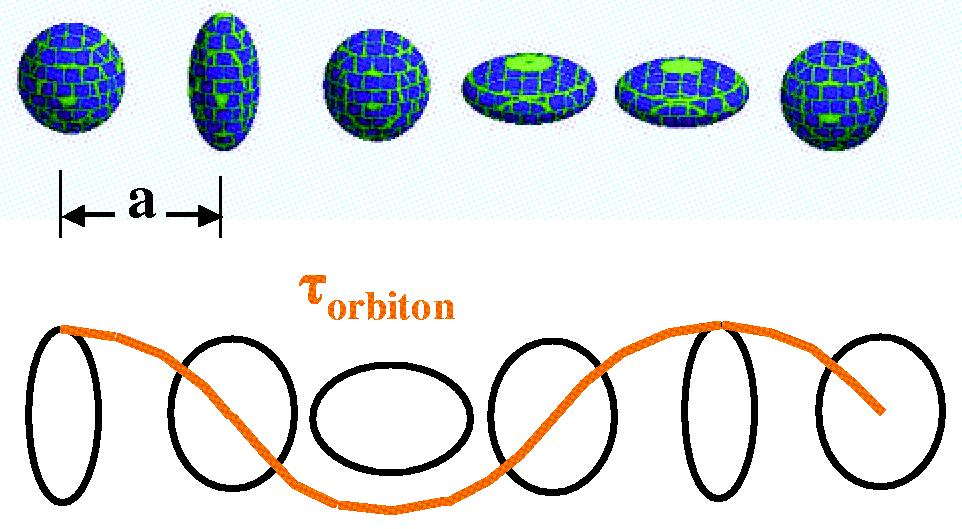
\includegraphics[angle=0, width=0.6\textwidth]{figsrc/orbiton.eps}%
\lthtmlpictureZ
\lthtmlcheckvsize\clearpage}

{\newpage\clearpage
\lthtmlpictureA{tex2html_wrap23107}%
\includegraphics[angle=0, width=0.5\textwidth]{figsrc/prcu2_0k0_5T.eps}%
\lthtmlpictureZ
\lthtmlcheckvsize\clearpage}

\stepcounter{section}
{\newpage\clearpage
\lthtmldisplayA{displaymath5082}%
\begin{displaymath}

\hat H_E(n)=\frac{a_0^2{\hat \mathbf p_n}^2}{2m_n} - \frac{1}{2} {\hat \mathbf u}^T_n \overline{K}(nn) {\hat \mathbf u}_n
\end{displaymath}%
\lthtmldisplayZ
\lthtmlcheckvsize\clearpage}

{\newpage\clearpage
\lthtmlinlinemathA{tex2html_wrap_inline6084}%
$\hat \mathbf u$%
\lthtmlinlinemathZ
\lthtmlcheckvsize\clearpage}

{\newpage\clearpage
\lthtmlinlinemathA{tex2html_wrap_inline6086}%
$\hat \mathbf u_n={\hat \mathbf P}_n/a_0=\Delta {\hat \mathbf r}_n/a_0$%
\lthtmlinlinemathZ
\lthtmlcheckvsize\clearpage}

{\newpage\clearpage
\lthtmlinlinemathA{tex2html_wrap_inline6088}%
$a_0=0.5219$%
\lthtmlinlinemathZ
\lthtmlcheckvsize\clearpage}

{\newpage\clearpage
\lthtmlinlinemathA{tex2html_wrap_inline6090}%
$m_n$%
\lthtmlinlinemathZ
\lthtmlcheckvsize\clearpage}

{\newpage\clearpage
\lthtmlinlinemathA{tex2html_wrap_inline6094}%
$\hat \mathbf p_n=d\hat \mathbf u_n/dt$%
\lthtmlinlinemathZ
\lthtmlcheckvsize\clearpage}

{\newpage\clearpage
\lthtmlinlinemathA{tex2html_wrap_inline6096}%
$\hat \mathbf u_n$%
\lthtmlinlinemathZ
\lthtmlcheckvsize\clearpage}

{\newpage\clearpage
\lthtmlinlinemathA{tex2html_wrap_inline6098}%
$\overline{K}(nn)$%
\lthtmlinlinemathZ
\lthtmlcheckvsize\clearpage}

{\newpage\clearpage
\lthtmldisplayA{displaymath5095}%
\begin{displaymath}
\hat H_{phon}=\sum_n \hat H_E(n) -\frac{1}{2} \sum_{n\neq n'} {\hat \mathbf u}_n^T \overline{K}(nn')  {\hat \mathbf u}_{n'}
\end{displaymath}%
\lthtmldisplayZ
\lthtmlcheckvsize\clearpage}

{\newpage\clearpage
\lthtmlinlinemathA{tex2html_wrap_inline6100}%
$K_{\alpha\beta}(nn')=-A_{\alpha\beta}(nn')$%
\lthtmlinlinemathZ
\lthtmlcheckvsize\clearpage}

{\newpage\clearpage
\lthtmlinlinemathA{tex2html_wrap_inline6102}%
$A_{\alpha\beta}$%
\lthtmlinlinemathZ
\lthtmlcheckvsize\clearpage}

{\newpage\clearpage
\lthtmldisplayA{displaymath5109}%
\begin{displaymath}

\hat H_E=\frac{a_0^2{\hat \mathbf p}^2}{2m} - \frac{1}{2} {\hat \mathbf u}^T \overline{K} {\hat \mathbf u} - {\mathbf F}^T {\hat \mathbf u}
\end{displaymath}%
\lthtmldisplayZ
\lthtmlcheckvsize\clearpage}

{\newpage\clearpage
\lthtmlinlinemathA{tex2html_wrap_inline6104}%
$\mathbf F$%
\lthtmlinlinemathZ
\lthtmlcheckvsize\clearpage}

{\newpage\clearpage
\lthtmlinlinemathA{tex2html_wrap_inline6106}%
$\mathbf H_{xc}$%
\lthtmlinlinemathZ
\lthtmlcheckvsize\clearpage}

{\newpage\clearpage
\lthtmlinlinemathA{tex2html_wrap_inline6112}%
$\overline{K}(nn')$%
\lthtmlinlinemathZ
\lthtmlcheckvsize\clearpage}

{\newpage\clearpage
\lthtmlinlinemathA{tex2html_wrap_inline6114}%
$\mathcal J(nn')$%
\lthtmlinlinemathZ
\lthtmlcheckvsize\clearpage}

{\newpage\clearpage
\lthtmlinlinemathA{tex2html_wrap_inline6116}%
$\overline{S}$%
\lthtmlinlinemathZ
\lthtmlcheckvsize\clearpage}

{\newpage\clearpage
\lthtmlinlinemathA{tex2html_wrap_inline6118}%
$\overline{K}=\overline{S}^T\overline{\Omega}\overline{S}$%
\lthtmlinlinemathZ
\lthtmlcheckvsize\clearpage}

{\newpage\clearpage
\lthtmldisplayA{displaymath5130}%
\begin{displaymath}
 \hat \mathbf u'=\overline{S} \hat \mathbf u +\overline{\Omega}^{-1} \overline{S} \mathbf F
\end{displaymath}%
\lthtmldisplayZ
\lthtmlcheckvsize\clearpage}

{\newpage\clearpage
\lthtmldisplayA{displaymath5136}%
\begin{displaymath}

\hat H_E=\frac{a_0^2{\hat \mathbf p}^{'2}}{2m}-\frac{1}{2} {\hat \mathbf u}^{'T} \overline{\Omega} {\hat \mathbf u'} 
-\frac{1}{2}\mathbf F^T  \mathbf u_0
\end{displaymath}%
\lthtmldisplayZ
\lthtmlcheckvsize\clearpage}

{\newpage\clearpage
\lthtmlinlinemathA{tex2html_wrap_inline6122}%
$\mathbf u_0=-\overline{S}^T\overline{\Omega}^{-1}\overline{S}\mathbf F$%
\lthtmlinlinemathZ
\lthtmlcheckvsize\clearpage}

{\newpage\clearpage
\lthtmlinlinemathA{tex2html_wrap_inline6124}%
$\overline{\Omega}$%
\lthtmlinlinemathZ
\lthtmlcheckvsize\clearpage}

{\newpage\clearpage
\lthtmlinlinemathA{tex2html_wrap_inline6126}%
$\Omega_{11}=-m a_0^2 (\Delta_1 /\hbar)^2$%
\lthtmlinlinemathZ
\lthtmlcheckvsize\clearpage}

{\newpage\clearpage
\lthtmlinlinemathA{tex2html_wrap_inline6128}%
$\Omega_{22}=-m a_0^2 (\Delta_2 /\hbar)^2$%
\lthtmlinlinemathZ
\lthtmlcheckvsize\clearpage}

{\newpage\clearpage
\lthtmlinlinemathA{tex2html_wrap_inline6130}%
$\Omega_{33}=-m a_0^2 (\Delta_3 /\hbar)^2$%
\lthtmlinlinemathZ
\lthtmlcheckvsize\clearpage}

{\newpage\clearpage
\lthtmlinlinemathA{tex2html_wrap_inline6132}%
$\Delta_1$%
\lthtmlinlinemathZ
\lthtmlcheckvsize\clearpage}

{\newpage\clearpage
\lthtmlinlinemathA{tex2html_wrap_indisplay23148}%
$\displaystyle \overline{\chi}^0$%
\lthtmlindisplaymathZ
\lthtmlcheckvsize\clearpage}

{\newpage\clearpage
\lthtmlinlinemathA{tex2html_wrap_indisplay23150}%
$\displaystyle \sum_{\nu\mu}\frac{\langle \nu|\hat \mathbf u|\mu\rangle\langle \mu |\hat \mathbf u^T|\nu \rangle}{\Delta_1 -\hbar \omega}
(p_{\nu} -p_{\mu})$%
\lthtmlindisplaymathZ
\lthtmlcheckvsize\clearpage}

{\newpage\clearpage
\lthtmlinlinemathA{tex2html_wrap_indisplay23152}%
$\displaystyle \sum_{\nu\mu}\frac{\langle \nu|\overline{S}^T \hat \mathbf u'|\mu\rangle\langle \mu |\hat \mathbf u'^T \overline{S}|\nu \rangle}{\Delta_1 -\hbar \omega}
(p_{\nu} -p_{\mu})$%
\lthtmlindisplaymathZ
\lthtmlcheckvsize\clearpage}

{\newpage\clearpage
\lthtmlinlinemathA{tex2html_wrap_inline6134}%
$\mathbf u'$%
\lthtmlinlinemathZ
\lthtmlcheckvsize\clearpage}

{\newpage\clearpage
\lthtmlinlinemathA{tex2html_wrap_inline6138}%
$u_1'$%
\lthtmlinlinemathZ
\lthtmlcheckvsize\clearpage}

{\newpage\clearpage
\lthtmlinlinemathA{tex2html_wrap_indisplay23157}%
$\displaystyle \chi^0_{\alpha\beta}$%
\lthtmlindisplaymathZ
\lthtmlcheckvsize\clearpage}

{\newpage\clearpage
\lthtmlinlinemathA{tex2html_wrap_indisplay23159}%
$\displaystyle S^T_{\alpha1}\sum_{\nu\mu}\frac{\langle \nu|\hat u_1'|\mu\rangle\langle \mu |\hat  u_1'|\nu \rangle}{\Delta_1 -\hbar \omega}
(p_{\nu} -p_{\mu}) S_{1\beta}$%
\lthtmlindisplaymathZ
\lthtmlcheckvsize\clearpage}

{\newpage\clearpage
\lthtmlinlinemathA{tex2html_wrap_indisplay23161}%
$\displaystyle S^T_{\alpha1}S_{1\beta}\frac{\hbar^2}{2ma_0^2\Delta_1}\left(\frac{1}{\Delta_1-\hbar\omega}+\frac{1}{\Delta_1+\hbar\omega}\right )$%
\lthtmlindisplaymathZ
\lthtmlcheckvsize\clearpage}

{\newpage\clearpage
\lthtmlinlinemathA{tex2html_wrap_inline6140}%
$\hat u_1'$%
\lthtmlinlinemathZ
\lthtmlcheckvsize\clearpage}

{\newpage\clearpage
\lthtmlinlinemathA{tex2html_wrap_inline6142}%
$\hat u_1'=a_0^{-1} \hbar/\sqrt{2m\Delta_1}(\hat a+\hat a^{\dagger})$%
\lthtmlinlinemathZ
\lthtmlcheckvsize\clearpage}

{\newpage\clearpage
\lthtmlinlinemathA{tex2html_wrap_inline6144}%
$\hat a^{\dagger}|\nu\rangle=\sqrt{\nu+1}|\nu+1\rangle$%
\lthtmlinlinemathZ
\lthtmlcheckvsize\clearpage}

{\newpage\clearpage
\lthtmlinlinemathA{tex2html_wrap_inline6146}%
$\hat a|\nu\rangle=\sqrt{\nu}|\nu-1\rangle$%
\lthtmlinlinemathZ
\lthtmlcheckvsize\clearpage}

{\newpage\clearpage
\lthtmlinlinemathA{tex2html_wrap_inline6148}%
$\sum_{\nu=0}^{\infty}(p_{\nu}-p_{\nu+1})(\nu+1)=1$%
\lthtmlinlinemathZ
\lthtmlcheckvsize\clearpage}

{\newpage\clearpage
\lthtmlinlinemathA{tex2html_wrap_inline6150}%
$p_{\nu}=exp(-\nu\Delta_1/kT)(1-exp(-\Delta_1/kT))$%
\lthtmlinlinemathZ
\lthtmlcheckvsize\clearpage}

{\newpage\clearpage
\lthtmlinlinemathA{tex2html_wrap_indisplay23171}%
$\displaystyle \sum_{i=1,2,3} S^T_{\alpha i}S_{i\beta}\frac{\hbar^2}{2ma_0^2\Delta_i}
\left(\frac{1}{\Delta_i-\hbar\omega}+\frac{1}{\Delta_i+\hbar\omega}\right )$%
\lthtmlindisplaymathZ
\lthtmlcheckvsize\clearpage}

\stepcounter{subsection}
{\newpage\clearpage
\lthtmlinlinemathA{tex2html_wrap_inline6152}%
$u_{max}$%
\lthtmlinlinemathZ
\lthtmlcheckvsize\clearpage}

{\newpage\clearpage
\lthtmlinlinemathA{tex2html_wrap_inline6154}%
$\langle \mathbf u \rangle$%
\lthtmlinlinemathZ
\lthtmlcheckvsize\clearpage}

{\newpage\clearpage
\lthtmlinlinemathA{tex2html_wrap_inline6156}%
$u \leftarrow u_{max} * tanh (u/u_{max})$%
\lthtmlinlinemathZ
\lthtmlcheckvsize\clearpage}

{\newpage\clearpage
\lthtmlinlinemathA{tex2html_wrap_inline6158}%
$\mathbf u$%
\lthtmlinlinemathZ
\lthtmlcheckvsize\clearpage}

{\newpage\clearpage
\lthtmlinlinemathA{tex2html_wrap_inline6160}%
$u_x,u_y,u_z$%
\lthtmlinlinemathZ
\lthtmlcheckvsize\clearpage}

{\newpage\clearpage
\lthtmlinlinemathA{tex2html_wrap_inline6164}%
$\mathbf y || \mathbf b$%
\lthtmlinlinemathZ
\lthtmlcheckvsize\clearpage}

{\newpage\clearpage
\lthtmlinlinemathA{tex2html_wrap_inline6166}%
$\mathbf z || \mathbf a \times \mathbf b $%
\lthtmlinlinemathZ
\lthtmlcheckvsize\clearpage}

{\newpage\clearpage
\lthtmlinlinemathA{tex2html_wrap_inline6168}%
$\mathbf x$%
\lthtmlinlinemathZ
\lthtmlcheckvsize\clearpage}

{\newpage\clearpage
\lthtmlinlinemathA{tex2html_wrap_inline6170}%
$\mathbf y$%
\lthtmlinlinemathZ
\lthtmlcheckvsize\clearpage}

{\newpage\clearpage
\lthtmlinlinemathA{tex2html_wrap_inline6172}%
$\mathbf z$%
\lthtmlinlinemathZ
\lthtmlcheckvsize\clearpage}

{\newpage\clearpage
\lthtmlinlinemathA{tex2html_wrap_inline6180}%
$n'$%
\lthtmlinlinemathZ
\lthtmlcheckvsize\clearpage}

{\newpage\clearpage
\lthtmlinlinemathA{tex2html_wrap_inline6182}%
$\hat H_{cf-phon}=\sum_{nn'}(\mathbf \nabla _{\hat \mathbf u(n')} B_l^m(n))   \mathbf u(n')  \hat O_{lm}(\hat \mathbf J_n)$%
\lthtmlinlinemathZ
\lthtmlcheckvsize\clearpage}

\stepcounter{section}
{\newpage\clearpage
\lthtmlinlinemathA{tex2html_wrap_inline6188}%
$\vec p_i$%
\lthtmlinlinemathZ
\lthtmlcheckvsize\clearpage}

{\newpage\clearpage
\lthtmlinlinemathA{tex2html_wrap_inline6190}%
$\vec U_i$%
\lthtmlinlinemathZ
\lthtmlcheckvsize\clearpage}

{\newpage\clearpage
\lthtmlinlinemathA{tex2html_wrap_inline6192}%
$c_L$%
\lthtmlinlinemathZ
\lthtmlcheckvsize\clearpage}

{\newpage\clearpage
\lthtmlinlinemathA{tex2html_wrap_inline6194}%
$c_T$%
\lthtmlinlinemathZ
\lthtmlcheckvsize\clearpage}

{\newpage\clearpage
\lthtmlinlinemathA{tex2html_wrap_indisplay23197}%
$\displaystyle H_{\rm ph}$%
\lthtmlindisplaymathZ
\lthtmlcheckvsize\clearpage}

{\newpage\clearpage
\lthtmlinlinemathA{tex2html_wrap_indisplay23199}%
$\displaystyle \sum_{i} \frac{a_0^2 \vec p_i^2}{2 m_i} +
\frac{1}{2}\sum_{ij} \frac{c_L(ij)-c_T(ij)}{2|\vec R_{ij}|^2}
(\vec U_j . \vec R_{ij}- \vec U_i . \vec R_{ij})^2$%
\lthtmlindisplaymathZ
\lthtmlcheckvsize\clearpage}

{\newpage\clearpage
\lthtmlinlinemathA{tex2html_wrap_indisplay23200}%
$\displaystyle + \frac{c_T(ij)}{2} (\vec U_j - \vec U_i )^2$%
\lthtmlindisplaymathZ
\lthtmlcheckvsize\clearpage}

{\newpage\clearpage
\lthtmlinlinemathA{tex2html_wrap_inline6196}%
$i,j$%
\lthtmlinlinemathZ
\lthtmlcheckvsize\clearpage}

{\newpage\clearpage
\lthtmlinlinemathA{tex2html_wrap_inline6198}%
$1/2$%
\lthtmlinlinemathZ
\lthtmlcheckvsize\clearpage}

{\newpage\clearpage
\lthtmlinlinemathA{tex2html_wrap_inline6200}%
$\vec R_{ij}=\vec R_{j}-\vec R_{i}$%
\lthtmlinlinemathZ
\lthtmlcheckvsize\clearpage}

{\newpage\clearpage
\lthtmlinlinemathA{tex2html_wrap_inline6204}%
$\bar \epsilon \vec R_i$%
\lthtmlinlinemathZ
\lthtmlcheckvsize\clearpage}

{\newpage\clearpage
\lthtmlinlinemathA{tex2html_wrap_inline6206}%
$\bar \omega \vec R_i$%
\lthtmlinlinemathZ
\lthtmlcheckvsize\clearpage}

{\newpage\clearpage
\lthtmlinlinemathA{tex2html_wrap_inline6208}%
$\vec P_i$%
\lthtmlinlinemathZ
\lthtmlcheckvsize\clearpage}

{\newpage\clearpage
\lthtmlinlinemathA{tex2html_wrap_inline6210}%
$\vec U_i = \bar \epsilon \vec R_i + \bar \omega \vec R_i+ \vec P_i= \bar a \vec R_i+ \vec P_i$%
\lthtmlinlinemathZ
\lthtmlcheckvsize\clearpage}

{\newpage\clearpage
\lthtmlinlinemathA{tex2html_wrap_indisplay23210}%
$\displaystyle (\vec U_j . \vec R_{ij}- \vec U_i . \vec R_{ij})^2$%
\lthtmlindisplaymathZ
\lthtmlcheckvsize\clearpage}

{\newpage\clearpage
\lthtmlinlinemathA{tex2html_wrap_indisplay23212}%
$\displaystyle (\vec R_{ij}^T\bar a \vec R_{ij}+ \vec R_{ij}^T \vec P_{ij})^2$%
\lthtmlindisplaymathZ
\lthtmlcheckvsize\clearpage}

{\newpage\clearpage
\lthtmlinlinemathA{tex2html_wrap_indisplay23214}%
$\displaystyle (\vec R_{ij}^T\bar a \vec R_{ij})^2 + 2 \vec R_{ij}^T\bar a \vec R_{ij}\vec R_{ij}^T \vec P_{ij}$%
\lthtmlindisplaymathZ
\lthtmlcheckvsize\clearpage}

{\newpage\clearpage
\lthtmlinlinemathA{tex2html_wrap_indisplay23215}%
$\displaystyle + (\vec R_{ij}^T \vec P_{ij})^2$%
\lthtmlindisplaymathZ
\lthtmlcheckvsize\clearpage}

{\newpage\clearpage
\lthtmlinlinemathA{tex2html_wrap_indisplay23217}%
$\displaystyle (\vec U_j - \vec U_i )^2$%
\lthtmlindisplaymathZ
\lthtmlcheckvsize\clearpage}

{\newpage\clearpage
\lthtmlinlinemathA{tex2html_wrap_indisplay23219}%
$\displaystyle \vec  R_{ij}^T\bar a^T\bar a \vec R_{ij}$%
\lthtmlindisplaymathZ
\lthtmlcheckvsize\clearpage}

{\newpage\clearpage
\lthtmlinlinemathA{tex2html_wrap_indisplay23220}%
$\displaystyle 2 \vec  R_{ij}^T\bar a^T\vec P_{ij} + \vec P_{ij}^T \vec P_{ij}$%
\lthtmlindisplaymathZ
\lthtmlcheckvsize\clearpage}

{\newpage\clearpage
\lthtmlinlinemathA{tex2html_wrap_inline6212}%
$\bar a$%
\lthtmlinlinemathZ
\lthtmlcheckvsize\clearpage}

{\newpage\clearpage
\lthtmlinlinemathA{tex2html_wrap_inline6214}%
$\vec P$%
\lthtmlinlinemathZ
\lthtmlcheckvsize\clearpage}

{\newpage\clearpage
\lthtmlinlinemathA{tex2html_wrap_inline6222}%
$H_{\rm E}$%
\lthtmlinlinemathZ
\lthtmlcheckvsize\clearpage}

{\newpage\clearpage
\lthtmlinlinemathA{tex2html_wrap_inline6224}%
$H_{\rm int}$%
\lthtmlinlinemathZ
\lthtmlcheckvsize\clearpage}

{\newpage\clearpage
\lthtmlinlinemathA{tex2html_wrap_indisplay23232}%
$\displaystyle E_{el} + H_{mix}+ H_{\rm E}+H_{\rm int}$%
\lthtmlindisplaymathZ
\lthtmlcheckvsize\clearpage}

\stepcounter{subsection}
{\newpage\clearpage
\lthtmlinlinemathA{tex2html_wrap_indisplay23238}%
$\displaystyle E_{el}$%
\lthtmlindisplaymathZ
\lthtmlcheckvsize\clearpage}

{\newpage\clearpage
\lthtmlinlinemathA{tex2html_wrap_indisplay23240}%
$\displaystyle \frac{1}{2}\sum_{ij} \frac{c_L(ij)-c_T(ij)}{2|\vec R_{ij}|^2}
(\vec R_{ij}^T\bar a \vec R_{ij})^2$%
\lthtmlindisplaymathZ
\lthtmlcheckvsize\clearpage}

{\newpage\clearpage
\lthtmlinlinemathA{tex2html_wrap_indisplay23241}%
$\displaystyle + \frac{c_T(ij)}{2} \vec  R_{ij}^T\bar a^T\bar a \vec R_{ij}$%
\lthtmlindisplaymathZ
\lthtmlcheckvsize\clearpage}

{\newpage\clearpage
\lthtmlinlinemathA{tex2html_wrap_indisplay23243}%
$\displaystyle \frac{1}{2} \sum_{ij,\alpha\beta\gamma\delta} \frac{c_L(ij)-c_T(ij)}{2|\vec R_{ij}|^2}
R_{ij}^{\alpha}R_{ij}^{\beta}R_{ij}^{\gamma}R_{ij}^{\delta}
a_{\alpha\beta}a_{\gamma\delta}$%
\lthtmlindisplaymathZ
\lthtmlcheckvsize\clearpage}

{\newpage\clearpage
\lthtmlinlinemathA{tex2html_wrap_indisplay23244}%
$\displaystyle + \frac{c_T(ij)}{2} R_{ij}^{\alpha} R_{ij}^{\delta}
a_{\alpha\beta} \delta_{\beta\gamma} a_{\gamma\delta}$%
\lthtmlindisplaymathZ
\lthtmlcheckvsize\clearpage}

{\newpage\clearpage
\lthtmlinlinemathA{tex2html_wrap_inline6234}%
$a_{\alpha\beta}$%
\lthtmlinlinemathZ
\lthtmlcheckvsize\clearpage}

{\newpage\clearpage
\lthtmlinlinemathA{tex2html_wrap_indisplay23247}%
$\displaystyle \frac{\partial E_{el}}{\partial a_{\alpha\beta}}$%
\lthtmlindisplaymathZ
\lthtmlcheckvsize\clearpage}

{\newpage\clearpage
\lthtmlinlinemathA{tex2html_wrap_indisplay23249}%
$\displaystyle \frac{1}{2}\sum_{ij,\gamma\delta} \frac{c_L(ij)-c_T(ij)}{|\vec R_{ij}|^2}
R_{ij}^{\alpha}R_{ij}^{\beta}R_{ij}^{\gamma}R_{ij}^{\delta}
a_{\gamma\delta}$%
\lthtmlindisplaymathZ
\lthtmlcheckvsize\clearpage}

{\newpage\clearpage
\lthtmlinlinemathA{tex2html_wrap_indisplay23250}%
$\displaystyle +    \frac{c_T(ij)}{2} R_{ij}^{\alpha}R_{ij}^{\delta}
\delta_{\beta\gamma} a_{\gamma\delta} +$%
\lthtmlindisplaymathZ
\lthtmlcheckvsize\clearpage}

{\newpage\clearpage
\lthtmlinlinemathA{tex2html_wrap_indisplay23251}%
$\displaystyle \frac{c_T(ij)}{2} R_{ij}^{\gamma} R_{ij}^{\beta}
a_{\gamma\delta} \delta_{\delta\alpha}$%
\lthtmlindisplaymathZ
\lthtmlcheckvsize\clearpage}

{\newpage\clearpage
\lthtmlinlinemathA{tex2html_wrap_inline6236}%
$\bar \epsilon$%
\lthtmlinlinemathZ
\lthtmlcheckvsize\clearpage}

{\newpage\clearpage
\lthtmlinlinemathA{tex2html_wrap_inline6238}%
$\epsilon_{\alpha\beta}=\epsilon_{\beta\alpha}$%
\lthtmlinlinemathZ
\lthtmlcheckvsize\clearpage}

{\newpage\clearpage
\lthtmlinlinemathA{tex2html_wrap_inline6240}%
$\omega_{\alpha\beta}=-\omega_{\beta\alpha}$%
\lthtmlinlinemathZ
\lthtmlcheckvsize\clearpage}

{\newpage\clearpage
\lthtmlinlinemathA{tex2html_wrap_inline6244}%
$\bar a=\bar \epsilon + \bar \omega$%
\lthtmlinlinemathZ
\lthtmlcheckvsize\clearpage}

{\newpage\clearpage
\lthtmlinlinemathA{tex2html_wrap_inline6246}%
$\epsilon_{\alpha\beta}$%
\lthtmlinlinemathZ
\lthtmlcheckvsize\clearpage}

{\newpage\clearpage
\lthtmlinlinemathA{tex2html_wrap_inline6248}%
$\alpha,\beta=1,2,3,\alpha \le \beta$%
\lthtmlinlinemathZ
\lthtmlcheckvsize\clearpage}

{\newpage\clearpage
\lthtmlinlinemathA{tex2html_wrap_indisplay23260}%
$\displaystyle \frac{\partial}{\partial \epsilon_{\alpha\beta}}$%
\lthtmlindisplaymathZ
\lthtmlcheckvsize\clearpage}

{\newpage\clearpage
\lthtmlinlinemathA{tex2html_wrap_indisplay23262}%
$\displaystyle \sum_{\gamma\delta=1,2,3}\frac{\partial a_{\gamma\delta}}{\partial \epsilon_{\alpha\beta}}
\frac{\partial}{\partial a_{\gamma\delta}}$%
\lthtmlindisplaymathZ
\lthtmlcheckvsize\clearpage}

{\newpage\clearpage
\lthtmlinlinemathA{tex2html_wrap_indisplay23264}%
$\displaystyle \frac{\partial}{\partial a_{\alpha\beta}} + (1-\delta_{\alpha\beta})
\frac{\partial}{\partial a_{\beta\alpha}}$%
\lthtmlindisplaymathZ
\lthtmlcheckvsize\clearpage}

{\newpage\clearpage
\lthtmlinlinemathA{tex2html_wrap_indisplay23266}%
$\displaystyle \frac{\partial E_{el}}{\partial \epsilon_{\alpha\beta}}$%
\lthtmlindisplaymathZ
\lthtmlcheckvsize\clearpage}

{\newpage\clearpage
\lthtmlinlinemathA{tex2html_wrap_indisplay23268}%
$\displaystyle \frac{\partial E_{el}}{\partial a_{\alpha\beta}} + \frac{\partial E_{el}}{\partial a_{\beta\alpha}}-\delta_{\alpha\beta}
\frac{\partial E_{el}}{\partial a_{\alpha\alpha}}$%
\lthtmlindisplaymathZ
\lthtmlcheckvsize\clearpage}

{\newpage\clearpage
\lthtmlinlinemathA{tex2html_wrap_indisplay23270}%
$\displaystyle \frac{1}{2}\sum_{ij,\gamma\delta} (2-\delta_{\alpha\beta})\frac{c_L(ij)-c_T(ij)}{|\vec R_{ij}|^2}
R_{ij}^{\alpha}R_{ij}^{\beta}R_{ij}^{\gamma}R_{ij}^{\delta}
a_{\gamma\delta}$%
\lthtmlindisplaymathZ
\lthtmlcheckvsize\clearpage}

{\newpage\clearpage
\lthtmlinlinemathA{tex2html_wrap_indisplay23271}%
$\displaystyle +    \frac{c_T(ij)}{2} a_{\gamma\delta} ( R_{ij}^{\alpha}R_{ij}^{\delta}
\delta_{\beta\gamma}  +   R_{ij}^{\gamma} R_{ij}^{\beta}
\delta_{\delta\alpha}$%
\lthtmlindisplaymathZ
\lthtmlcheckvsize\clearpage}

{\newpage\clearpage
\lthtmlinlinemathA{tex2html_wrap_indisplay23272}%
$\displaystyle +    R_{ij}^{\beta} R_{ij}^{\delta}
\delta_{\alpha\gamma}  +   R_{ij}^{\gamma}R_{ij}^{\alpha}
\delta_{\delta\beta}$%
\lthtmlindisplaymathZ
\lthtmlcheckvsize\clearpage}

{\newpage\clearpage
\lthtmlinlinemathA{tex2html_wrap_indisplay23273}%
$\displaystyle -    R_{ij}^{\alpha}R_{ij}^{\delta}
\delta_{\alpha\beta}\delta_{\beta\gamma}    -  R_{ij}^{\gamma} R_{ij}^{\beta}
\delta_{\delta\alpha} \delta_{\alpha\beta} )$%
\lthtmlindisplaymathZ
\lthtmlcheckvsize\clearpage}

{\newpage\clearpage
\lthtmlinlinemathA{tex2html_wrap_indisplay23275}%
$\displaystyle c^{\alpha\beta\gamma\delta}$%
\lthtmlindisplaymathZ
\lthtmlcheckvsize\clearpage}

{\newpage\clearpage
\lthtmlinlinemathA{tex2html_wrap_indisplay23277}%
$\displaystyle \frac{\partial^2E_{el}}{\partial \epsilon_{\alpha\beta} \partial \epsilon_{\gamma\delta}}$%
\lthtmlindisplaymathZ
\lthtmlcheckvsize\clearpage}

{\newpage\clearpage
\lthtmlinlinemathA{tex2html_wrap_indisplay23279}%
$\displaystyle \frac{1}{2}\sum_{ij}(2-\delta_{\alpha\beta})(2-\delta_{\gamma\delta}) \frac{c_L(ij)-c_T(ij)}{|\vec R_{ij}|^2}
R_{ij}^{\alpha}R_{ij}^{\beta}R_{ij}^{\gamma}R_{ij}^{\delta}$%
\lthtmlindisplaymathZ
\lthtmlcheckvsize\clearpage}

{\newpage\clearpage
\lthtmlinlinemathA{tex2html_wrap_indisplay23280}%
$\displaystyle +    c_T(ij)  ( R_{ij}^{\alpha}R_{ij}^{\delta}
\delta_{\beta\gamma}  +   R_{ij}^{\gamma}R_{ij}^{\beta}
\delta_{\delta\alpha}$%
\lthtmlindisplaymathZ
\lthtmlcheckvsize\clearpage}

{\newpage\clearpage
\lthtmlinlinemathA{tex2html_wrap_indisplay23282}%
$\displaystyle -    R_{ij}^{\alpha}R_{ij}^{\delta}
\delta_{\alpha\beta}\delta_{\beta\gamma}    -  R_{ij}^{\gamma}R_{ij}^{\alpha}
\delta_{\delta\alpha} \delta_{\alpha\beta} +$%
\lthtmlindisplaymathZ
\lthtmlcheckvsize\clearpage}

{\newpage\clearpage
\lthtmlinlinemathA{tex2html_wrap_indisplay23283}%
$\displaystyle -    R_{ij}^{\beta}R_{ij}^{\alpha}
\delta_{\alpha\gamma} \delta_{\gamma\delta}  -   R_{ij}^{\gamma}R_{ij}^{\alpha}
\delta_{\delta\beta}\delta_{\gamma\delta}$%
\lthtmlindisplaymathZ
\lthtmlcheckvsize\clearpage}

{\newpage\clearpage
\lthtmlinlinemathA{tex2html_wrap_indisplay23284}%
$\displaystyle +    R_{ij}^{\alpha}R_{ij}^{\alpha}
\delta_{\alpha\beta}\delta_{\beta\gamma} \delta_{\gamma\delta}   )$%
\lthtmlindisplaymathZ
\lthtmlcheckvsize\clearpage}

{\newpage\clearpage
\lthtmlinlinemathA{tex2html_wrap_indisplay23288}%
$\displaystyle \frac{1}{2}\sum_{\alpha\beta\gamma\delta} c^{\alpha\beta\gamma\delta} \epsilon_{\alpha\beta}\epsilon_{\gamma\delta}$%
\lthtmlindisplaymathZ
\lthtmlcheckvsize\clearpage}

{\newpage\clearpage
\lthtmlinlinemathA{tex2html_wrap_inline6250}%
$\bar \omega$%
\lthtmlinlinemathZ
\lthtmlcheckvsize\clearpage}

{\newpage\clearpage
\lthtmlinlinemathA{tex2html_wrap_inline6252}%
$R^{\alpha}R^{\delta}\omega_{\sigma}
\epsilon_{\sigma\alpha\beta}\delta_{\beta\gamma}\omega_{\eta}\epsilon_{\eta\gamma\delta}=
R^{\alpha}R^{\delta}\omega_{\sigma} \omega_{\eta}
\epsilon_{\sigma\alpha\beta}\epsilon_{\eta\beta\delta}=
R^{\alpha}R^{\delta}\omega_{\sigma} \omega_{\eta}
(\delta_{\sigma\delta}\delta_{\alpha\eta}-\delta_{\sigma\eta}\delta_{\alpha\delta})=
(\vec R . \vec \omega)^2-R^2\omega^2 \neq 0$%
\lthtmlinlinemathZ
\lthtmlcheckvsize\clearpage}

{\newpage\clearpage
\lthtmlinlinemathA{tex2html_wrap_inline6254}%
$\vec R$%
\lthtmlinlinemathZ
\lthtmlcheckvsize\clearpage}

{\newpage\clearpage
\lthtmlinlinemathA{tex2html_wrap_indisplay23297}%
$\displaystyle \sum_{\gamma\delta=1,2,3,\gamma \le \delta} c^{\alpha\beta\gamma\delta} \epsilon_{\gamma\delta}$%
\lthtmlindisplaymathZ
\lthtmlcheckvsize\clearpage}

{\newpage\clearpage
\lthtmlinlinemathA{tex2html_wrap_indisplay23299}%
$\displaystyle \epsilon_1$%
\lthtmlindisplaymathZ
\lthtmlcheckvsize\clearpage}

{\newpage\clearpage
\lthtmlinlinemathA{tex2html_wrap_indisplay23301}%
$\displaystyle \epsilon_{11}$%
\lthtmlindisplaymathZ
\lthtmlcheckvsize\clearpage}

{\newpage\clearpage
\lthtmlinlinemathA{tex2html_wrap_indisplay23302}%
$\displaystyle \epsilon_2$%
\lthtmlindisplaymathZ
\lthtmlcheckvsize\clearpage}

{\newpage\clearpage
\lthtmlinlinemathA{tex2html_wrap_indisplay23304}%
$\displaystyle \epsilon_{22}$%
\lthtmlindisplaymathZ
\lthtmlcheckvsize\clearpage}

{\newpage\clearpage
\lthtmlinlinemathA{tex2html_wrap_indisplay23305}%
$\displaystyle \epsilon_3$%
\lthtmlindisplaymathZ
\lthtmlcheckvsize\clearpage}

{\newpage\clearpage
\lthtmlinlinemathA{tex2html_wrap_indisplay23307}%
$\displaystyle \epsilon_{33}$%
\lthtmlindisplaymathZ
\lthtmlcheckvsize\clearpage}

{\newpage\clearpage
\lthtmlinlinemathA{tex2html_wrap_indisplay23308}%
$\displaystyle \epsilon_4$%
\lthtmlindisplaymathZ
\lthtmlcheckvsize\clearpage}

{\newpage\clearpage
\lthtmlinlinemathA{tex2html_wrap_indisplay23310}%
$\displaystyle 2\epsilon_{23}=2\epsilon_{32}$%
\lthtmlindisplaymathZ
\lthtmlcheckvsize\clearpage}

{\newpage\clearpage
\lthtmlinlinemathA{tex2html_wrap_indisplay23311}%
$\displaystyle \epsilon_5$%
\lthtmlindisplaymathZ
\lthtmlcheckvsize\clearpage}

{\newpage\clearpage
\lthtmlinlinemathA{tex2html_wrap_indisplay23313}%
$\displaystyle 2\epsilon_{31}=2\epsilon_{13}$%
\lthtmlindisplaymathZ
\lthtmlcheckvsize\clearpage}

{\newpage\clearpage
\lthtmlinlinemathA{tex2html_wrap_indisplay23314}%
$\displaystyle \epsilon_6$%
\lthtmlindisplaymathZ
\lthtmlcheckvsize\clearpage}

{\newpage\clearpage
\lthtmlinlinemathA{tex2html_wrap_indisplay23316}%
$\displaystyle 2\epsilon_{12}=2\epsilon_{21}$%
\lthtmlindisplaymathZ
\lthtmlcheckvsize\clearpage}

{\newpage\clearpage
\lthtmlinlinemathA{tex2html_wrap_indisplay23318}%
$\displaystyle c^{11}$%
\lthtmlindisplaymathZ
\lthtmlcheckvsize\clearpage}

{\newpage\clearpage
\lthtmlinlinemathA{tex2html_wrap_indisplay23320}%
$\displaystyle c^{1111}$%
\lthtmlindisplaymathZ
\lthtmlcheckvsize\clearpage}

{\newpage\clearpage
\lthtmlinlinemathA{tex2html_wrap_indisplay23321}%
$\displaystyle c^{44}$%
\lthtmlindisplaymathZ
\lthtmlcheckvsize\clearpage}

{\newpage\clearpage
\lthtmlinlinemathA{tex2html_wrap_indisplay23323}%
$\displaystyle c^{2323}$%
\lthtmlindisplaymathZ
\lthtmlcheckvsize\clearpage}

{\newpage\clearpage
\lthtmlinlinemathA{tex2html_wrap_inline6256}%
$c^{\alpha\beta}$%
\lthtmlinlinemathZ
\lthtmlcheckvsize\clearpage}

{\newpage\clearpage
\lthtmlinlinemathA{tex2html_wrap_inline6258}%
$\beta=1,...,6$%
\lthtmlinlinemathZ
\lthtmlcheckvsize\clearpage}

{\newpage\clearpage
\lthtmlinlinemathA{tex2html_wrap_inline6260}%
$\alpha \le \beta$%
\lthtmlinlinemathZ
\lthtmlcheckvsize\clearpage}

{\newpage\clearpage
\lthtmlinlinemathA{tex2html_wrap_inline6262}%
$c^{\alpha\beta}=c^{\beta\alpha}$%
\lthtmlinlinemathZ
\lthtmlcheckvsize\clearpage}

{\newpage\clearpage
\lthtmlinlinemathA{tex2html_wrap_inline6264}%
$c^{\alpha\beta\gamma\delta}=c^{\beta\alpha\gamma\delta}=c^{\alpha\beta\delta\gamma}$%
\lthtmlinlinemathZ
\lthtmlcheckvsize\clearpage}

{\newpage\clearpage
\lthtmlinlinemathA{tex2html_wrap_indisplay23332}%
$\displaystyle \frac{1}{2}\sum_{\alpha\gamma=1,..,6} c^{\alpha\gamma} \epsilon_{\alpha}\epsilon_{\gamma}$%
\lthtmlindisplaymathZ
\lthtmlcheckvsize\clearpage}

\stepcounter{subsection}
{\newpage\clearpage
\lthtmlinlinemathA{tex2html_wrap_indisplay23337}%
$\displaystyle H_{mix}$%
\lthtmlindisplaymathZ
\lthtmlcheckvsize\clearpage}

{\newpage\clearpage
\lthtmlinlinemathA{tex2html_wrap_indisplay23339}%
$\displaystyle \frac{1}{2} \sum_{ij} \frac{c_L(ij)-c_T(ij)}{|\vec R_{ij}|^2}
\vec R_{ij}^T\bar a \vec R_{ij}\vec R_{ij}^T \vec P_{ij}$%
\lthtmlindisplaymathZ
\lthtmlcheckvsize\clearpage}

{\newpage\clearpage
\lthtmlinlinemathA{tex2html_wrap_indisplay23340}%
$\displaystyle + c_T(ij) \vec  R_{ij}^T\bar a^T\vec P_{ij}$%
\lthtmlindisplaymathZ
\lthtmlcheckvsize\clearpage}

{\newpage\clearpage
\lthtmlinlinemathA{tex2html_wrap_indisplay23342}%
$\displaystyle \frac{1}{2}\sum_{ij} 2\frac{c_L(ij)-c_T(ij)}{|\vec R_{ij}|^2}
\vec R_{ij}^T\bar a \vec R_{ij}\vec R_{ij}^T \vec P_{i}$%
\lthtmlindisplaymathZ
\lthtmlcheckvsize\clearpage}

{\newpage\clearpage
\lthtmlinlinemathA{tex2html_wrap_indisplay23343}%
$\displaystyle + 2 c_T(ij) \vec  R_{ij}^T\bar a^T\vec P_{i}$%
\lthtmlindisplaymathZ
\lthtmlcheckvsize\clearpage}

{\newpage\clearpage
\lthtmlinlinemathA{tex2html_wrap_indisplay23345}%
$\displaystyle \sum_{ij,\alpha\beta} \frac{c_L(ij)-c_T(ij)}{|\vec R_{ij}|^2}
R_{ij}^{\alpha} a_{\alpha\beta} R_{ij}^{\beta} R_{ij}^{\gamma}  P_{i}^{\gamma}$%
\lthtmlindisplaymathZ
\lthtmlcheckvsize\clearpage}

{\newpage\clearpage
\lthtmlinlinemathA{tex2html_wrap_indisplay23346}%
$\displaystyle +  c_T(ij)   R_{ij}^{\beta} a_{\alpha\beta} \delta_{\alpha\gamma} P_{i}^{\gamma}$%
\lthtmlindisplaymathZ
\lthtmlcheckvsize\clearpage}

{\newpage\clearpage
\lthtmlinlinemathA{tex2html_wrap_indisplay23348}%
$\displaystyle -\sum_{\stackrel{i,\alpha=1,..,6}{ \gamma=1,2,3}} G_{mix}^{\alpha\gamma}(i) \epsilon_{\alpha} P_{i}^{\gamma}/a_0 +
\sum_{ij,\alpha\beta}  c_T(ij)   R_{ij}^{\beta} \omega_{\alpha\beta} P_{i}^{\alpha}$%
\lthtmlindisplaymathZ
\lthtmlcheckvsize\clearpage}

{\newpage\clearpage
\lthtmlinlinemathA{tex2html_wrap_inline6272}%
$\langle P_i \rangle$%
\lthtmlinlinemathZ
\lthtmlcheckvsize\clearpage}

{\newpage\clearpage
\lthtmlinlinemathA{tex2html_wrap_inline6274}%
$G_{mix}^{\alpha\gamma}(i)$%
\lthtmlinlinemathZ
\lthtmlcheckvsize\clearpage}

{\newpage\clearpage
\lthtmlinlinemathA{tex2html_wrap_inline6276}%
$\alpha=(\alpha\beta)$%
\lthtmlinlinemathZ
\lthtmlcheckvsize\clearpage}

{\newpage\clearpage
\lthtmlinlinemathA{tex2html_wrap_indisplay23354}%
$\displaystyle G_{mix}^{(\alpha\beta)\gamma}(i)$%
\lthtmlindisplaymathZ
\lthtmlcheckvsize\clearpage}

{\newpage\clearpage
\lthtmlinlinemathA{tex2html_wrap_indisplay23356}%
$\displaystyle -a_0\sum_{j} \frac{c_L(ij)-c_T(ij)}{|\vec R_{ij}|^2}
R_{ij}^{\alpha} R_{ij}^{\beta} R_{ij}^{\gamma} -$%
\lthtmlindisplaymathZ
\lthtmlcheckvsize\clearpage}

{\newpage\clearpage
\lthtmlinlinemathA{tex2html_wrap_indisplay23357}%
$\displaystyle -a_0\frac{1}{2}\sum_{j}  c_T(ij)   (R_{ij}^{\beta}  \delta_{\alpha\gamma}+
R_{ij}^{\alpha}  \delta_{\beta\gamma})$%
\lthtmlindisplaymathZ
\lthtmlcheckvsize\clearpage}

\stepcounter{subsection}
{\newpage\clearpage
\lthtmlinlinemathA{tex2html_wrap_indisplay23362}%
$\displaystyle (\vec R_{ij}^T \vec P_{ij})^2$%
\lthtmlindisplaymathZ
\lthtmlcheckvsize\clearpage}

{\newpage\clearpage
\lthtmlinlinemathA{tex2html_wrap_indisplay23364}%
$\displaystyle \sum_{\alpha,\beta=1,2,3} R_{ij}^{\alpha}R_{ij}^{\beta}(P_{j}^{\alpha}-P_{i}^{\alpha})(P_{j}^{\beta}-P_{i}^{\beta})$%
\lthtmlindisplaymathZ
\lthtmlcheckvsize\clearpage}

{\newpage\clearpage
\lthtmlinlinemathA{tex2html_wrap_indisplay23366}%
$\displaystyle \vec P_{ij}^T \vec P_{ij}$%
\lthtmlindisplaymathZ
\lthtmlcheckvsize\clearpage}

{\newpage\clearpage
\lthtmlinlinemathA{tex2html_wrap_indisplay23368}%
$\displaystyle \sum_{\alpha=1,2,3} (P_{j}^{\alpha}-P_{i}^{\alpha})^2$%
\lthtmlindisplaymathZ
\lthtmlcheckvsize\clearpage}

{\newpage\clearpage
\lthtmlinlinemathA{tex2html_wrap_indisplay23370}%
$\displaystyle \sum_{\alpha=1,2,3} (P_{j}^{\alpha})^2 +(P_{i}^{\alpha})^2- 2 P_{i}^{\alpha} P_{j}^{\alpha}$%
\lthtmlindisplaymathZ
\lthtmlcheckvsize\clearpage}

{\newpage\clearpage
\lthtmlinlinemathA{tex2html_wrap_indisplay23373}%
$\displaystyle H_{\rm E}$%
\lthtmlindisplaymathZ
\lthtmlcheckvsize\clearpage}

{\newpage\clearpage
\lthtmlinlinemathA{tex2html_wrap_indisplay23375}%
$\displaystyle \sum_{i} H_{\rm E}(i)$%
\lthtmlindisplaymathZ
\lthtmlcheckvsize\clearpage}

{\newpage\clearpage
\lthtmlinlinemathA{tex2html_wrap_indisplay23376}%
$\displaystyle H_{\rm E}(i)$%
\lthtmlindisplaymathZ
\lthtmlcheckvsize\clearpage}

{\newpage\clearpage
\lthtmlinlinemathA{tex2html_wrap_indisplay23377}%
$\textstyle \equiv$%
\lthtmlindisplaymathZ
\lthtmlcheckvsize\clearpage}

{\newpage\clearpage
\lthtmlinlinemathA{tex2html_wrap_indisplay23378}%
$\displaystyle \frac{a_0^2 \vec p_i^2}{2 m_i} -\frac{1}{2}
\sum_{\alpha} K_{\alpha\beta}(ii) P_{i}^{\alpha}P_{i}^{\beta}a_0^{-2}$%
\lthtmlindisplaymathZ
\lthtmlcheckvsize\clearpage}

{\newpage\clearpage
\lthtmlinlinemathA{tex2html_wrap_indisplay23379}%
$\displaystyle K_{\alpha\beta}(ii)$%
\lthtmlindisplaymathZ
\lthtmlcheckvsize\clearpage}

{\newpage\clearpage
\lthtmlinlinemathA{tex2html_wrap_indisplay23381}%
$\displaystyle -a_0^2\sum_{j} \frac{R_{ij}^{\alpha}R_{ij}^{\beta}}{|\vec R_{ij}|^2}
[c_L(ij)-c_T(ij)] +$%
\lthtmlindisplaymathZ
\lthtmlcheckvsize\clearpage}

{\newpage\clearpage
\lthtmlinlinemathA{tex2html_wrap_indisplay23382}%
$\displaystyle +  \delta_{\alpha\beta} c_T(ij)$%
\lthtmlindisplaymathZ
\lthtmlcheckvsize\clearpage}

{\newpage\clearpage
\lthtmlinlinemathA{tex2html_wrap_indisplay23385}%
$\displaystyle H_{\rm int}$%
\lthtmlindisplaymathZ
\lthtmlcheckvsize\clearpage}

{\newpage\clearpage
\lthtmlinlinemathA{tex2html_wrap_indisplay23387}%
$\displaystyle -\frac{1}{2}\sum_{i\ne j,\alpha\beta} K_{\alpha\beta}(ij) P_{i}^{\alpha}P_{j}^{\beta}a_0^{-2}$%
\lthtmlindisplaymathZ
\lthtmlcheckvsize\clearpage}

{\newpage\clearpage
\lthtmlinlinemathA{tex2html_wrap_indisplay23388}%
$\displaystyle K_{\alpha\beta}(ij)$%
\lthtmlindisplaymathZ
\lthtmlcheckvsize\clearpage}

{\newpage\clearpage
\lthtmlinlinemathA{tex2html_wrap_indisplay23390}%
$\displaystyle a_0^2\frac{R_{ij}^{\alpha}R_{ij}^{\beta}}{|\vec R_{ij}|^2}[c_L(ij)-c_T(ij)]
+a_0^2\delta_{\alpha\beta}c_T(ij)$%
\lthtmlindisplaymathZ
\lthtmlcheckvsize\clearpage}

\stepcounter{subsection}
{\newpage\clearpage
\lthtmlinlinemathA{tex2html_wrap_inline6296}%
$lm$%
\lthtmlinlinemathZ
\lthtmlcheckvsize\clearpage}

{\newpage\clearpage
\lthtmlinlinemathA{tex2html_wrap_inline6300}%
$i=1,...,N_{\rm nuclei}$%
\lthtmlinlinemathZ
\lthtmlcheckvsize\clearpage}

{\newpage\clearpage
\lthtmlinlinemathA{tex2html_wrap_inline6302}%
$j$%
\lthtmlinlinemathZ
\lthtmlcheckvsize\clearpage}

{\newpage\clearpage
\lthtmlinlinemathA{tex2html_wrap_inline6304}%
$j=N_{\rm nuclei}+1,... N_{\rm nuclei}+N_{\rm magnetic ions}$%
\lthtmlinlinemathZ
\lthtmlcheckvsize\clearpage}

{\newpage\clearpage
\lthtmlinlinemathA{tex2html_wrap_indisplay23403}%
$\displaystyle H$%
\lthtmlindisplaymathZ
\lthtmlcheckvsize\clearpage}

{\newpage\clearpage
\lthtmlinlinemathA{tex2html_wrap_indisplay23405}%
$\displaystyle H_{\rm ph} +\sum_{j,\gamma} B_{\gamma}(j,\vec U_1,...,\vec U_N) O_{\gamma}(\vec J_i)$%
\lthtmlindisplaymathZ
\lthtmlcheckvsize\clearpage}

{\newpage\clearpage
\lthtmlinlinemathA{tex2html_wrap_indisplay23407}%
$\displaystyle H_{\rm ph} +\sum_{j,\gamma} B_{\gamma}(j,0,\dots,0) O_{\gamma}(\vec J_j) + H_{\rm cfph}$%
\lthtmlindisplaymathZ
\lthtmlcheckvsize\clearpage}

{\newpage\clearpage
\lthtmlinlinemathA{tex2html_wrap_indisplay23409}%
$\displaystyle H_{\rm cfph}$%
\lthtmlindisplaymathZ
\lthtmlcheckvsize\clearpage}

{\newpage\clearpage
\lthtmlinlinemathA{tex2html_wrap_indisplay23411}%
$\displaystyle \sum_{i<j,\gamma}\nabla_{\vec U_i} B_{\gamma}(j) \vec U_i O_{\gamma}(\vec J_j)$%
\lthtmlindisplaymathZ
\lthtmlcheckvsize\clearpage}

{\newpage\clearpage
\lthtmlinlinemathA{tex2html_wrap_indisplay23413}%
$\displaystyle \sum_{i<j,\gamma}\nabla_{\vec U_i} B_{\gamma}(j) (\bar a \vec R_i + \vec P_i)O_{\gamma}(\vec J_j)$%
\lthtmlindisplaymathZ
\lthtmlcheckvsize\clearpage}

{\newpage\clearpage
\lthtmlinlinemathA{tex2html_wrap_indisplay23415}%
$\displaystyle \sum_{i<j,\alpha\beta=1,2,3,\gamma=1,...} R_i^{\beta}  \frac{\partial B_{\gamma}(j)}{\partial U_i^{\alpha}}
\epsilon_{\alpha\beta} O_{\gamma}(\vec J_j)$%
\lthtmlindisplaymathZ
\lthtmlcheckvsize\clearpage}

{\newpage\clearpage
\lthtmlinlinemathA{tex2html_wrap_indisplay23416}%
$\displaystyle +\sum_{i<j,\gamma}\nabla_{\vec U_j} B_{\gamma}(j) \vec P_i O_{\gamma}(\vec J_j)$%
\lthtmlindisplaymathZ
\lthtmlcheckvsize\clearpage}

{\newpage\clearpage
\lthtmlinlinemathA{tex2html_wrap_indisplay23418}%
$\displaystyle -\sum_{j,\alpha=1,..,6,\gamma=1,...} G_{\rm cfph}^{\alpha\gamma}(j) \epsilon_{\alpha} O_{\gamma}(\vec J_j)$%
\lthtmlindisplaymathZ
\lthtmlcheckvsize\clearpage}

{\newpage\clearpage
\lthtmlinlinemathA{tex2html_wrap_indisplay23419}%
$\displaystyle -\sum_{i<j,\alpha=1,2,3,\gamma=1,...} \Gamma^{\alpha\gamma}(ij) P_i^{\alpha}a_0^{-1} O_{\gamma}(\vec J_j)$%
\lthtmlindisplaymathZ
\lthtmlcheckvsize\clearpage}

{\newpage\clearpage
\lthtmlinlinemathA{tex2html_wrap_indisplay23422}%
$\displaystyle G_{\rm cfph}^{(\alpha\beta)\gamma}(j)$%
\lthtmlindisplaymathZ
\lthtmlcheckvsize\clearpage}

{\newpage\clearpage
\lthtmlinlinemathA{tex2html_wrap_indisplay23424}%
$\displaystyle -\frac{1}{2}\sum_{i}( R_i^{\beta}  \frac{\partial B_{\gamma}(j)}{\partial U_i^{\alpha}}
+ R_i^{\alpha} \frac{\partial B_{\gamma}(j)}{\partial U_i^{\beta}} )$%
\lthtmlindisplaymathZ
\lthtmlcheckvsize\clearpage}

{\newpage\clearpage
\lthtmlinlinemathA{tex2html_wrap_indisplay23426}%
$\displaystyle \Gamma^{\alpha\gamma}(ij)$%
\lthtmlindisplaymathZ
\lthtmlcheckvsize\clearpage}

{\newpage\clearpage
\lthtmlinlinemathA{tex2html_wrap_indisplay23428}%
$\displaystyle -a_0\frac{\partial B_{\gamma}(j)}{\partial U_i^{\alpha}}$%
\lthtmlindisplaymathZ
\lthtmlcheckvsize\clearpage}

{\newpage\clearpage
\lthtmlinlinemathA{tex2html_wrap_inline6312}%
$\mathbf u = \mathbf P / a_0$%
\lthtmlinlinemathZ
\lthtmlcheckvsize\clearpage}

{\newpage\clearpage
\lthtmlinlinemathA{tex2html_wrap_indisplay23435}%
$\displaystyle \sum_{i,\gamma} B_{\gamma}(i,0,\dots,0) O_{\gamma}(\vec J_i) + \sum_{i} H_{\rm E}(i) +$%
\lthtmlindisplaymathZ
\lthtmlcheckvsize\clearpage}

{\newpage\clearpage
\lthtmlinlinemathA{tex2html_wrap_indisplay23436}%
$\textstyle +$%
\lthtmlindisplaymathZ
\lthtmlcheckvsize\clearpage}

{\newpage\clearpage
\lthtmlinlinemathA{tex2html_wrap_indisplay23437}%
$\displaystyle \frac{1}{2}\sum_{\alpha\gamma=1-6} c^{\alpha\gamma} \epsilon_{\alpha}\epsilon_{\gamma} -$%
\lthtmlindisplaymathZ
\lthtmlcheckvsize\clearpage}

{\newpage\clearpage
\lthtmlinlinemathA{tex2html_wrap_indisplay23438}%
$\textstyle -$%
\lthtmlindisplaymathZ
\lthtmlcheckvsize\clearpage}

{\newpage\clearpage
\lthtmlinlinemathA{tex2html_wrap_indisplay23439}%
$\displaystyle \frac{1}{2}\sum_{i\ne j,\alpha\beta} K_{\alpha\beta}(ij) u_{i}^{\alpha}u_{j}^{\beta}
-\sum_{i<j,\alpha=1-6,\gamma}\Gamma^{\alpha\gamma}(ij) u^{\alpha}_i O_{\gamma}(\vec J_j)$%
\lthtmlindisplaymathZ
\lthtmlcheckvsize\clearpage}

{\newpage\clearpage
\lthtmlinlinemathA{tex2html_wrap_indisplay23441}%
$\displaystyle \sum_{i,\alpha=1-6,\gamma=1,2,3} G_{mix}^{\alpha\gamma}(i) \epsilon_{\alpha} u_{i}^{\gamma} -$%
\lthtmlindisplaymathZ
\lthtmlcheckvsize\clearpage}

{\newpage\clearpage
\lthtmlinlinemathA{tex2html_wrap_indisplay23443}%
$\displaystyle \sum_{i,\alpha=1-6,\gamma=1,...} G_{\rm cfph}^{\alpha\gamma}(i) \epsilon_{\alpha} O_{\gamma}(\vec J_i)$%
\lthtmlindisplaymathZ
\lthtmlcheckvsize\clearpage}

{\newpage\clearpage
\lthtmlinlinemathA{tex2html_wrap_inline6316}%
$\langle O_l^m(i) \rangle $%
\lthtmlinlinemathZ
\lthtmlcheckvsize\clearpage}

{\newpage\clearpage
\lthtmlinlinemathA{tex2html_wrap_inline6318}%
$\langle \vec u_i \rangle$%
\lthtmlinlinemathZ
\lthtmlcheckvsize\clearpage}

{\newpage\clearpage
\lthtmlinlinemathA{tex2html_wrap_indisplay23449}%
$\displaystyle 0$%
\lthtmlindisplaymathZ
\lthtmlcheckvsize\clearpage}

{\newpage\clearpage
\lthtmlinlinemathA{tex2html_wrap_indisplay23451}%
$\displaystyle \sum_{ij} \frac{c_L(ij)-c_T(ij)}{|\vec R_{ij}|^2}
(\vec R_{ij}^T\bar \epsilon \vec R_{ij})R_{ij}^{\alpha}R_{ij}^{\beta}$%
\lthtmlindisplaymathZ
\lthtmlcheckvsize\clearpage}

{\newpage\clearpage
\lthtmlinlinemathA{tex2html_wrap_indisplay23452}%
$\displaystyle + \frac{c_T(ij)}{2} (R_{ij}^{\alpha} (\bar \epsilon \vec R_{ij})^{\beta}+R_{ij}^{\beta} (\bar \epsilon R_{ij})^{\alpha})$%
\lthtmlindisplaymathZ
\lthtmlcheckvsize\clearpage}

{\newpage\clearpage
\lthtmlinlinemathA{tex2html_wrap_indisplay23453}%
$\displaystyle +2\sum_{ij} \frac{c_L(ij)-c_T(ij)}{|\vec R_{ij}|^2}
R_{ij}^{\alpha}R_{ij}^{\beta} \vec R_{ij}^T \langle \vec P_{i} \rangle$%
\lthtmlindisplaymathZ
\lthtmlcheckvsize\clearpage}

{\newpage\clearpage
\lthtmlinlinemathA{tex2html_wrap_indisplay23454}%
$\displaystyle +2 c_T(ij) \vec  R_{ij}^{\beta} \langle P_{i}^{\alpha} \rangle
+ \sum_{ij,\gamma}\frac{\partial B_{\gamma}(i)}{\partial U_j^{\alpha}}   R_j^{\beta}  \langle O_{\gamma}(\vec J_i) \rangle$%
\lthtmlindisplaymathZ
\lthtmlcheckvsize\clearpage}

{\newpage\clearpage
\lthtmlinlinemathA{tex2html_wrap_inline6324}%
$\alpha,\beta=1,2,3$%
\lthtmlinlinemathZ
\lthtmlcheckvsize\clearpage}

{\newpage\clearpage
\lthtmlinlinemathA{tex2html_wrap_inline6332}%
$\alpha=1,...,6$%
\lthtmlinlinemathZ
\lthtmlcheckvsize\clearpage}

{\newpage\clearpage
\lthtmlinlinemathA{tex2html_wrap_indisplay23462}%
$\displaystyle \sum_{\gamma=1,..6}  c^{\alpha\gamma} \epsilon_{\gamma}$%
\lthtmlindisplaymathZ
\lthtmlcheckvsize\clearpage}

{\newpage\clearpage
\lthtmlinlinemathA{tex2html_wrap_indisplay23464}%
$\displaystyle \sum_{i,\gamma=1,2,3}  G_{mix}^{\alpha\gamma}(i)\langle u_{i}^{\gamma} \rangle$%
\lthtmlindisplaymathZ
\lthtmlcheckvsize\clearpage}

{\newpage\clearpage
\lthtmlinlinemathA{tex2html_wrap_indisplay23466}%
$\displaystyle \sum_{i,\gamma=1,...} G_{\rm cfph}^{\alpha\gamma}(i) \langle O_{\gamma}(\vec J_i) \rangle$%
\lthtmlindisplaymathZ
\lthtmlcheckvsize\clearpage}

\stepcounter{subsection}
{\newpage\clearpage
\lthtmlinlinemathA{tex2html_wrap_inline6334}%
$\langle u_{j}^{\alpha} \rangle$%
\lthtmlinlinemathZ
\lthtmlcheckvsize\clearpage}

{\newpage\clearpage
\lthtmlinlinemathA{tex2html_wrap_inline6336}%
$\langle O_{\gamma}(\vec J_i) \rangle$%
\lthtmlinlinemathZ
\lthtmlcheckvsize\clearpage}

{\newpage\clearpage
\lthtmlinlinemathA{tex2html_wrap_inline6342}%
$G_{mix}$%
\lthtmlinlinemathZ
\lthtmlcheckvsize\clearpage}

{\newpage\clearpage
\lthtmlinlinemathA{tex2html_wrap_inline6344}%
$G_{\rm cfph}$%
\lthtmlinlinemathZ
\lthtmlcheckvsize\clearpage}

{\newpage\clearpage
\lthtmlinlinemathA{tex2html_wrap_inline6346}%
$\Gamma_{\rm cfph}$%
\lthtmlinlinemathZ
\lthtmlcheckvsize\clearpage}

{\newpage\clearpage
\lthtmlinlinemathA{tex2html_wrap_inline6350}%
$\Delta L/L$%
\lthtmlinlinemathZ
\lthtmlcheckvsize\clearpage}

{\newpage\clearpage
\lthtmldisplayA{displaymath5994}%
\begin{displaymath}
\frac{\Delta L}{L}=\sum_{\alpha\beta} \epsilon_{\alpha\beta} \hat L_{\alpha} \hat L_{\beta}
\end{displaymath}%
\lthtmldisplayZ
\lthtmlcheckvsize\clearpage}

{\newpage\clearpage
\lthtmlinlinemathA{tex2html_wrap_inline6352}%
$\hat \mathbf L$%
\lthtmlinlinemathZ
\lthtmlcheckvsize\clearpage}

\stepcounter{section}
{\newpage\clearpage
\lthtmlinlinemathA{tex2html_wrap_inline7476}%
$\hat J_a,\hat J_b,\hat J_c,\hat O_{2-2},\hat O_{2-1},\hat O_{20},\hat O_{21},\hat O_{22},\hat O_{3-3}...\hat O_{66},\hat J_a^2,\hat J_b^2,\hat J_c^2,\hat J_a^4,\hat J_b^4,\hat J_c^4$%
\lthtmlinlinemathZ
\lthtmlcheckvsize\clearpage}

{\newpage\clearpage
\lthtmlinlinemathA{tex2html_wrap_inline7478}%
$\hat J_a,\hat J_b,\hat J_c,\hat O_{2-2},\hat O_{2-1},\hat O_{20},\hat O_{21},\hat O_{22},\hat O_{3-3}...\hat O_{66}$%
\lthtmlinlinemathZ
\lthtmlcheckvsize\clearpage}

{\newpage\clearpage
\lthtmlinlinemathA{tex2html_wrap_inline7480}%
$\hat J_a,\hat J_b,\hat J_c$%
\lthtmlinlinemathZ
\lthtmlcheckvsize\clearpage}

{\newpage\clearpage
\lthtmlinlinemathA{tex2html_wrap_inline7484}%
$\hat u_a,\hat u_b,\hat u_c$%
\lthtmlinlinemathZ
\lthtmlcheckvsize\clearpage}

{\newpage\clearpage
\lthtmlinlinemathA{tex2html_wrap_inline7496}%
$\hat S_a,\hat S_b,\hat S_c,\hat L_a,\hat L_b,\hat L_c,\hat T_2^{-2},\hat T_2^{-1},\hat T_2^{0},\hat T_2^{1},\hat T_2^{2},\hat T_3^{-3}...\hat T_6^{6}$%
\lthtmlinlinemathZ
\lthtmlcheckvsize\clearpage}

{\newpage\clearpage
\lthtmlinlinemathA{tex2html_wrap_inline7500}%
$\hat J_a,\hat J_b,\hat J_c,\hat O_{2-2},\hat O_{2-1},\hat O_{20},\hat O_{21},\hat O_{22},\hat O_{4-4}...,\hat O_{44},\hat O_{6-6}...\hat O_{66}$%
\lthtmlinlinemathZ
\lthtmlcheckvsize\clearpage}

{\newpage\clearpage
\lthtmlinlinemathA{tex2html_wrap_inline7502}%
$J$%
\lthtmlinlinemathZ
\lthtmlcheckvsize\clearpage}

{\newpage\clearpage
\lthtmlinlinemathA{tex2html_wrap_inline7504}%
$\hat I_1$%
\lthtmlinlinemathZ
\lthtmlcheckvsize\clearpage}

{\newpage\clearpage
\lthtmlinlinemathA{tex2html_wrap_inline7506}%
$\hat J_x$%
\lthtmlinlinemathZ
\lthtmlcheckvsize\clearpage}

{\newpage\clearpage
\lthtmlinlinemathA{tex2html_wrap_inline7508}%
$\hat I_1 \equiv 5 \hat O_4^4 + O_4^0$%
\lthtmlinlinemathZ
\lthtmlcheckvsize\clearpage}

{\newpage\clearpage
\lthtmlinlinemathA{tex2html_wrap_inline7510}%
$I_n$%
\lthtmlinlinemathZ
\lthtmlcheckvsize\clearpage}

{\newpage\clearpage
\lthtmlinlinemathA{tex2html_wrap_inline7514}%
$M(\mathbf Q)$%
\lthtmlinlinemathZ
\lthtmlcheckvsize\clearpage}

\stepcounter{subsection}
\stepcounter{subsection}
{\newpage\clearpage
\lthtmlinlinemathA{tex2html_wrap_inline7516}%
$Z(K')$%
\lthtmlinlinemathZ
\lthtmlcheckvsize\clearpage}

\stepcounter{subsection}
\stepcounter{subsection}
{\newpage\clearpage
\lthtmlinlinemathA{tex2html_wrap_inline7518}%
$10^{-14}$%
\lthtmlinlinemathZ
\lthtmlcheckvsize\clearpage}

\stepcounter{subsection}
\stepcounter{subsection}
\stepcounter{section}
{\newpage\clearpage
\lthtmlinlinemathA{tex2html_wrap_inline7522}%
$\langle \hat \mathbf I \rangle$%
\lthtmlinlinemathZ
\lthtmlcheckvsize\clearpage}

{\newpage\clearpage
\lthtmlinlinemathA{tex2html_wrap_inline7524}%
$\langle -|\hat \mathbf I|+\rangle\sqrt{(p_--p_+)}$%
\lthtmlinlinemathZ
\lthtmlcheckvsize\clearpage}

{\newpage\clearpage
\lthtmlinlinemathA{tex2html_wrap_inline7526}%
$\langle\hat \mathbf M\rangle$%
\lthtmlinlinemathZ
\lthtmlcheckvsize\clearpage}

{\newpage\clearpage
\lthtmlinlinemathA{tex2html_wrap_inline7528}%
$\langle-| \hat\mathbf M|+\rangle\sqrt{(p_--p_+)}$%
\lthtmlinlinemathZ
\lthtmlcheckvsize\clearpage}

{\newpage\clearpage
\lthtmlinlinemathA{tex2html_wrap_inline7530}%
$\langle \hat \mathbf L\rangle$%
\lthtmlinlinemathZ
\lthtmlcheckvsize\clearpage}

{\newpage\clearpage
\lthtmlinlinemathA{tex2html_wrap_inline7532}%
$\langle-| \hat\mathbf L|+\rangle\sqrt{(p_--p_+)}$%
\lthtmlinlinemathZ
\lthtmlcheckvsize\clearpage}

{\newpage\clearpage
\lthtmlinlinemathA{tex2html_wrap_inline7534}%
$\langle \hat\mathbf S\rangle$%
\lthtmlinlinemathZ
\lthtmlcheckvsize\clearpage}

{\newpage\clearpage
\lthtmlinlinemathA{tex2html_wrap_inline7536}%
$\langle-|\hat \mathbf S|+\rangle\sqrt{(p_--p_+)}$%
\lthtmlinlinemathZ
\lthtmlcheckvsize\clearpage}

{\newpage\clearpage
\lthtmlinlinemathA{tex2html_wrap_inline7538}%
$\langle\hat \mathbf M(\mathbf Q)\rangle$%
\lthtmlinlinemathZ
\lthtmlcheckvsize\clearpage}

{\newpage\clearpage
\lthtmlinlinemathA{tex2html_wrap_inline7540}%
$\langle-|\hat \mathbf M(\mathbf Q)|+\rangle\sqrt{(p_--p_+)}$%
\lthtmlinlinemathZ
\lthtmlcheckvsize\clearpage}

{\newpage\clearpage
\lthtmlinlinemathA{tex2html_wrap_inline7542}%
$\hat \mathbf R$%
\lthtmlinlinemathZ
\lthtmlcheckvsize\clearpage}

{\newpage\clearpage
\lthtmlinlinemathA{tex2html_wrap_inline7544}%
$\langle \hat \mathbf P\rangle$%
\lthtmlinlinemathZ
\lthtmlcheckvsize\clearpage}

{\newpage\clearpage
\lthtmlinlinemathA{tex2html_wrap_inline7546}%
$\langle-|\hat \mathbf P|+\rangle\sqrt{(p_--p_+)}$%
\lthtmlinlinemathZ
\lthtmlcheckvsize\clearpage}

{\newpage\clearpage
\lthtmlinlinemathA{tex2html_wrap_inline7548}%
$-|e|Z_l^m(\Omega)R^2(r)$%
\lthtmlinlinemathZ
\lthtmlcheckvsize\clearpage}

{\newpage\clearpage
\lthtmlinlinemathA{tex2html_wrap_inline7550}%
$\langle\sum_i Z_l^m(\Omega_i)\rangle$%
\lthtmlinlinemathZ
\lthtmlcheckvsize\clearpage}

{\newpage\clearpage
\lthtmlinlinemathA{tex2html_wrap_inline7552}%
$\langle-|\sum_i Z_l^m(\Omega_i)|+\rangle\sqrt{(p_--p_+)}$%
\lthtmlinlinemathZ
\lthtmlcheckvsize\clearpage}

{\newpage\clearpage
\lthtmlinlinemathA{tex2html_wrap_inline7554}%
$Z_l^m(\Omega)R^2(r)$%
\lthtmlinlinemathZ
\lthtmlcheckvsize\clearpage}

{\newpage\clearpage
\lthtmlinlinemathA{tex2html_wrap_inline7556}%
$|$%
\lthtmlinlinemathZ
\lthtmlcheckvsize\clearpage}

{\newpage\clearpage
\lthtmlinlinemathA{tex2html_wrap_inline7560}%
$Z_l^m(\Omega)F(r)$%
\lthtmlinlinemathZ
\lthtmlcheckvsize\clearpage}

{\newpage\clearpage
\lthtmlinlinemathA{tex2html_wrap_inline7564}%
$H_2||\vec b$%
\lthtmlinlinemathZ
\lthtmlcheckvsize\clearpage}

{\newpage\clearpage
\lthtmlinlinemathA{tex2html_wrap_inline7566}%
$H_3||(\vec a \times \vec b)$%
\lthtmlinlinemathZ
\lthtmlcheckvsize\clearpage}

{\newpage\clearpage
\lthtmlinlinemathA{tex2html_wrap_inline7568}%
$H_1$%
\lthtmlinlinemathZ
\lthtmlcheckvsize\clearpage}

{\newpage\clearpage
\lthtmlinlinemathA{tex2html_wrap_inline7570}%
$H_2$%
\lthtmlinlinemathZ
\lthtmlcheckvsize\clearpage}

{\newpage\clearpage
\lthtmlinlinemathA{tex2html_wrap_inline7572}%
$H_3$%
\lthtmlinlinemathZ
\lthtmlcheckvsize\clearpage}

\stepcounter{subsection}
\stepcounter{subsubsection}
{\newpage\clearpage
\lthtmlinlinemathA{tex2html_wrap_inline7584}%
${\hat \mathbf I}$%
\lthtmlinlinemathZ
\lthtmlcheckvsize\clearpage}

{\newpage\clearpage
\lthtmlinlinemathA{tex2html_wrap_inline7592}%
$\mathbf H_{ext}$%
\lthtmlinlinemathZ
\lthtmlcheckvsize\clearpage}

{\newpage\clearpage
\lthtmlinlinemathA{tex2html_wrap_inline7594}%
$\langle\hat I_a\rangle, \langle\hat  I_b\rangle,\langle\hat  I_c\rangle etc$%
\lthtmlinlinemathZ
\lthtmlcheckvsize\clearpage}

{\newpage\clearpage
\lthtmlinlinemathA{tex2html_wrap_inline7596}%
$\mathbf I$%
\lthtmlinlinemathZ
\lthtmlcheckvsize\clearpage}

{\newpage\clearpage
\lthtmlinlinemathA{tex2html_wrap_inline7598}%
$\hat H=\hat H_0- \hat \mathbf M \mathbf H_{ext} - \hat I_a {\rm Hxc}(1) - \hat I_b {\rm Hxc}(2) -\hat I_c {\rm Hxc}(3) 
-\hat I_d {\rm Hxc}(4) ...$%
\lthtmlinlinemathZ
\lthtmlcheckvsize\clearpage}

{\newpage\clearpage
\lthtmlinlinemathA{tex2html_wrap_inline7600}%
$Z=\sum_i e^{-\epsilon_i/kT}$%
\lthtmlinlinemathZ
\lthtmlcheckvsize\clearpage}

{\newpage\clearpage
\lthtmlinlinemathA{tex2html_wrap_inline7602}%
$U=\sum_i p_i=\sum_i \epsilon_i e^{-\epsilon_i/kT}/Z$%
\lthtmlinlinemathZ
\lthtmlcheckvsize\clearpage}

{\newpage\clearpage
\lthtmlinlinemathA{tex2html_wrap_inline7604}%
$T<0$%
\lthtmlinlinemathZ
\lthtmlcheckvsize\clearpage}

{\newpage\clearpage
\lthtmlinlinemathA{tex2html_wrap_inline7608}%
$n=(-T)$%
\lthtmlinlinemathZ
\lthtmlcheckvsize\clearpage}

{\newpage\clearpage
\lthtmlinlinemathA{tex2html_wrap_inline7610}%
$p_n=1$%
\lthtmlinlinemathZ
\lthtmlcheckvsize\clearpage}

\stepcounter{subsubsection}
\stepcounter{subsubsection}
{\newpage\clearpage
\lthtmlinlinemathA{tex2html_wrap_inline7612}%
$M^s_{\alpha\beta}$%
\lthtmlinlinemathZ
\lthtmlcheckvsize\clearpage}

{\newpage\clearpage
\lthtmlinlinemathA{tex2html_wrap_inline7614}%
$|-\rangle \rightarrow |+\rangle$%
\lthtmlinlinemathZ
\lthtmlcheckvsize\clearpage}

{\newpage\clearpage
\lthtmlinlinemathA{tex2html_wrap_inline7622}%
$M$%
\lthtmlinlinemathZ
\lthtmlcheckvsize\clearpage}

{\newpage\clearpage
\lthtmlinlinemathA{tex2html_wrap_inline7624}%
$u1$%
\lthtmlinlinemathZ
\lthtmlcheckvsize\clearpage}

{\newpage\clearpage
\lthtmlinlinemathA{tex2html_wrap_inline7626}%
${\mathbf u^s_{\alpha1}}=\sqrt{(p_--p_+)}\langle -|I^s_{\alpha}-\langle I^s_{\alpha}\rangle_{\mathbf H,T}|+\rangle$%
\lthtmlinlinemathZ
\lthtmlcheckvsize\clearpage}

{\newpage\clearpage
\lthtmlinlinemathA{tex2html_wrap_inline7628}%
${\mathcal U^s_{\alpha1}}$%
\lthtmlinlinemathZ
\lthtmlcheckvsize\clearpage}

{\newpage\clearpage
\lthtmlinlinemathA{tex2html_wrap_inline7630}%
${\mathbf u^s_{\alpha1}}$%
\lthtmlinlinemathZ
\lthtmlcheckvsize\clearpage}

{\newpage\clearpage
\lthtmlinlinemathA{tex2html_wrap_inline7636}%
${\mathbf u^s_{\alpha1}}=\sqrt{(p_--p_+)}\langle -|\hat I^s_{\alpha}-\langle \hat I^s_{\alpha}\rangle_{\mathbf H,T}|+\rangle$%
\lthtmlinlinemathZ
\lthtmlcheckvsize\clearpage}

{\newpage\clearpage
\lthtmlinlinemathA{tex2html_wrap_inline7638}%
$\Delta(tn)=0$%
\lthtmlinlinemathZ
\lthtmlcheckvsize\clearpage}

{\newpage\clearpage
\lthtmlinlinemathA{tex2html_wrap_inline7640}%
$(p_--p_+)$%
\lthtmlinlinemathZ
\lthtmlcheckvsize\clearpage}

{\newpage\clearpage
\lthtmlinlinemathA{tex2html_wrap_inline7642}%
$(p_+/kT)$%
\lthtmlinlinemathZ
\lthtmlcheckvsize\clearpage}

{\newpage\clearpage
\lthtmlinlinemathA{tex2html_wrap_inline7646}%
$\Delta=-10^{-10}$%
\lthtmlinlinemathZ
\lthtmlcheckvsize\clearpage}

\stepcounter{subsubsection}
\stepcounter{subsection}
\stepcounter{subsubsection}
{\newpage\clearpage
\lthtmlinlinemathA{tex2html_wrap_inline7666}%
$\mathbf m$%
\lthtmlinlinemathZ
\lthtmlcheckvsize\clearpage}

\stepcounter{subsubsection}
{\newpage\clearpage
\lthtmlinlinemathA{tex2html_wrap_inline7678}%
$\mu_B$%
\lthtmlinlinemathZ
\lthtmlcheckvsize\clearpage}

{\newpage\clearpage
\lthtmlinlinemathA{tex2html_wrap_inline7680}%
$m1$%
\lthtmlinlinemathZ
\lthtmlcheckvsize\clearpage}

{\newpage\clearpage
\lthtmlinlinemathA{tex2html_wrap_inline7682}%
${\rm m1}^s_{\alpha}=\sqrt{(p_--p_+)}\langle -|\hat m^s_{\alpha}-\langle\hat  m^s_{\alpha}\rangle_{\mathbf H,T}|+\rangle$%
\lthtmlinlinemathZ
\lthtmlcheckvsize\clearpage}

{\newpage\clearpage
\lthtmlinlinemathA{tex2html_wrap_inline7684}%
${\mathbf m1^s_{\alpha}}=\sqrt{(p_--p_+)}\langle -|\hat m^s_{\alpha}-\langle\hat  m^s_{\alpha}\rangle_{\mathbf H,T}|+\rangle$%
\lthtmlinlinemathZ
\lthtmlcheckvsize\clearpage}

{\newpage\clearpage
\lthtmlinlinemathA{tex2html_wrap_inline7686}%
$\hat \mathbf m=2\hat \mathbf S+ \hat \mathbf L $%
\lthtmlinlinemathZ
\lthtmlcheckvsize\clearpage}

\stepcounter{subsubsection}
\stepcounter{subsubsection}
{\newpage\clearpage
\lthtmlinlinemathA{tex2html_wrap_inline7706}%
$L1$%
\lthtmlinlinemathZ
\lthtmlcheckvsize\clearpage}

{\newpage\clearpage
\lthtmlinlinemathA{tex2html_wrap_inline7708}%
${\rm L1}^s_{\alpha}=\sqrt{(p_--p_+)}\langle -|\hat L^s_{\alpha}-\langle\hat  L^s_{\alpha}\rangle_{\mathbf H,T}|+\rangle$%
\lthtmlinlinemathZ
\lthtmlcheckvsize\clearpage}

\stepcounter{subsubsection}
\stepcounter{subsubsection}
{\newpage\clearpage
\lthtmlinlinemathA{tex2html_wrap_inline7712}%
$S1$%
\lthtmlinlinemathZ
\lthtmlcheckvsize\clearpage}

{\newpage\clearpage
\lthtmlinlinemathA{tex2html_wrap_inline7714}%
${\rm S1}^s_{\alpha}=\sqrt{(p_--p_+)}\langle -|\hat S^s_{\alpha}-\langle \hat S^s_{\alpha}\rangle_{\mathbf H,T}|+\rangle$%
\lthtmlinlinemathZ
\lthtmlcheckvsize\clearpage}

\stepcounter{subsubsection}
{\newpage\clearpage
\lthtmlinlinemathA{tex2html_wrap_inline7716}%
$\hat \mathcal Q$%
\lthtmlinlinemathZ
\lthtmlcheckvsize\clearpage}

{\newpage\clearpage
\lthtmlinlinemathA{tex2html_wrap_inline7718}%
$\mathbf M(\mathbf r)$%
\lthtmlinlinemathZ
\lthtmlcheckvsize\clearpage}

{\newpage\clearpage
\lthtmldisplayA{displaymath7106}%
\begin{displaymath}

  \mathbf Q \times (\hat \mathcal Q \times  \mathbf Q) = \frac{-1}{2\mu_B} 
   \mathbf Q \times (\hat \mathbf M(\mathbf Q) \times \mathbf Q) =\frac{-1}{2\mu_B} \int d\mathbf r
e^{i\mathbf Q \mathbf r} \left [ 
     \mathbf Q \times (\hat \mathbf M(\mathbf r) \times \mathbf Q) \right ]
 \end{displaymath}%
\lthtmldisplayZ
\lthtmlcheckvsize\clearpage}

{\newpage\clearpage
\lthtmlinlinemathA{tex2html_wrap_inline7720}%
$\hat \mathbf M(\mathbf r)=\hat \mathbf M_S(\mathbf r)+\hat \mathbf M_L(\mathbf r)$%
\lthtmlinlinemathZ
\lthtmlcheckvsize\clearpage}

{\newpage\clearpage
\lthtmlinlinemathA{tex2html_wrap_inline7722}%
$\nabla \times \hat \mathbf M_L (\mathbf r)=\hat \mathbf j(\mathbf r)$%
\lthtmlinlinemathZ
\lthtmlcheckvsize\clearpage}

{\newpage\clearpage
\lthtmlinlinemathA{tex2html_wrap_inline7724}%
$\hat \mathbf M(\mathbf r)$%
\lthtmlinlinemathZ
\lthtmlcheckvsize\clearpage}

{\newpage\clearpage
\lthtmlinlinemathA{tex2html_wrap_inline7728}%
$\mathbf Q \times \mathbf Q \times \mathbf Q=0$%
\lthtmlinlinemathZ
\lthtmlcheckvsize\clearpage}

{\newpage\clearpage
\lthtmlinlinemathA{tex2html_wrap_inline7732}%
$\langle \hat \mathcal Q^{d \dag }_{\alpha} \rangle_{T,H}$%
\lthtmlinlinemathZ
\lthtmlcheckvsize\clearpage}

\stepcounter{subsubsection}
{\newpage\clearpage
\lthtmlinlinemathA{tex2html_wrap_inline7734}%
${\mathbf m^s_{\alpha1}}(\mathbf Q)=\sqrt{(p_--p_+)}
\langle -|\hat \mathbf M_{\alpha}^{\dag }(\mathbf Q)-\langle \hat \mathbf M_{\alpha}^{\dag }(\mathbf Q)\rangle|+\rangle/\mu_B$%
\lthtmlinlinemathZ
\lthtmlcheckvsize\clearpage}

{\newpage\clearpage
\lthtmlinlinemathA{tex2html_wrap_inline7736}%
$\hat \mathcal Q_{\alpha}=\frac{\hat  \mathbf M_{\alpha}(\mathbf Q)}{-2 \mu_B}$%
\lthtmlinlinemathZ
\lthtmlcheckvsize\clearpage}

{\newpage\clearpage
\lthtmlinlinemathA{tex2html_wrap_inline7740}%
$\alpha=1,..3$%
\lthtmlinlinemathZ
\lthtmlcheckvsize\clearpage}

{\newpage\clearpage
\lthtmlinlinemathA{tex2html_wrap_inline7744}%
${\mathbf m^s_{\alpha1}}(\mathbf Q)$%
\lthtmlinlinemathZ
\lthtmlcheckvsize\clearpage}

\stepcounter{subsubsection}
{\newpage\clearpage
\lthtmlinlinemathA{tex2html_wrap_inline7760}%
${{\mathbf r\mathbf i\mathbf x\mathbf s}^s_{\alpha1}}(\mathbf Q)=\sqrt{(p_--p_+)}
\langle -|\hat \mathbf R_{\alpha}^{\dag }(\mathbf Q)-\langle \hat \mathbf R_{\alpha}^{\dag }(\mathbf Q)\rangle|+\rangle$%
\lthtmlinlinemathZ
\lthtmlcheckvsize\clearpage}

{\newpage\clearpage
\lthtmlinlinemathA{tex2html_wrap_inline7762}%
$\hat R_{\alpha}$%
\lthtmlinlinemathZ
\lthtmlcheckvsize\clearpage}

{\newpage\clearpage
\lthtmlinlinemathA{tex2html_wrap_inline7764}%
$\alpha= xx, xy ,xz, yx, yy, yz, zx,zy, zz$%
\lthtmlinlinemathZ
\lthtmlcheckvsize\clearpage}

{\newpage\clearpage
\lthtmlinlinemathA{tex2html_wrap_inline7768}%
$\alpha=1,..9$%
\lthtmlinlinemathZ
\lthtmlcheckvsize\clearpage}

{\newpage\clearpage
\lthtmlinlinemathA{tex2html_wrap_inline7772}%
${{\mathbf r\mathbf i\mathbf x\mathbf s}^s_{\alpha1}}(\mathbf Q)$%
\lthtmlinlinemathZ
\lthtmlcheckvsize\clearpage}

\stepcounter{subsubsection}
\stepcounter{subsubsection}
{\newpage\clearpage
\lthtmlinlinemathA{tex2html_wrap_inline7790}%
$P_{\alpha}$%
\lthtmlinlinemathZ
\lthtmlcheckvsize\clearpage}

{\newpage\clearpage
\lthtmlinlinemathA{tex2html_wrap_inline7792}%
$\langle-|\hat P_{\alpha}|+\rangle=S_{i\alpha}\frac{\hbar}{\sqrt{2m\Delta_i}}$%
\lthtmlinlinemathZ
\lthtmlcheckvsize\clearpage}

{\newpage\clearpage
\lthtmlinlinemathA{tex2html_wrap_inline7798}%
${\rm P1}^s_{\alpha}=\sqrt{(p_--p_+)}\langle -|\hat P^s_{\alpha}-\langle\hat  P^s_{\alpha}\rangle_{\mathbf H,T}|+\rangle$%
\lthtmlinlinemathZ
\lthtmlcheckvsize\clearpage}

{\newpage\clearpage
\lthtmlinlinemathA{tex2html_wrap_inline7800}%
$\langle-|\hat P_{\alpha}|+\rangle=S_{tn,\alpha}\frac{\hbar}{\sqrt{2m\Delta_{tn}}}$%
\lthtmlinlinemathZ
\lthtmlcheckvsize\clearpage}

{\newpage\clearpage
\lthtmlinlinemathA{tex2html_wrap_inline7802}%
${\mathbf P1^s_{\alpha}}=\sqrt{(p_--p_+)}\langle -|\hat P^s_{\alpha}-\langle\hat  P^s_{\alpha}\rangle_{\mathbf H,T}|+\rangle$%
\lthtmlinlinemathZ
\lthtmlcheckvsize\clearpage}

\stepcounter{subsubsection}
{\newpage\clearpage
\lthtmlinlinemathA{tex2html_wrap_inline7820}%
$-|e|Z_l^m R^2(r)$%
\lthtmlinlinemathZ
\lthtmlcheckvsize\clearpage}

\stepcounter{subsubsection}
{\newpage\clearpage
\lthtmlinlinemathA{tex2html_wrap_inline7832}%
$\sum_i \hat Z_{lm}(\Omega_i)$%
\lthtmlinlinemathZ
\lthtmlcheckvsize\clearpage}

{\newpage\clearpage
\lthtmlinlinemathA{tex2html_wrap_inline7834}%
$cd1$%
\lthtmlinlinemathZ
\lthtmlcheckvsize\clearpage}

{\newpage\clearpage
\lthtmlinlinemathA{tex2html_wrap_inline7836}%
${\rm cd1}^s_{\alpha=lm}=\sqrt{(p_--p_+)}\langle -|\sum_i \hat  Z^s_{lm}(\Omega_i)-\langle \sum_i\hat  Z^s_{lm}(\Omega_i)\rangle_{\mathbf H,T}|+\rangle$%
\lthtmlinlinemathZ
\lthtmlcheckvsize\clearpage}

\stepcounter{subsubsection}
{\newpage\clearpage
\lthtmlinlinemathA{tex2html_wrap_inline7838}%
$Z_l^m R^2(r)$%
\lthtmlinlinemathZ
\lthtmlcheckvsize\clearpage}

{\newpage\clearpage
\lthtmlinlinemathA{tex2html_wrap_inline7840}%
$M^S_{x,y,z}=\sum_{l,m} a^{x,y,z}_{S,lm} Z_l^m R^2(r)$%
\lthtmlinlinemathZ
\lthtmlcheckvsize\clearpage}

{\newpage\clearpage
\lthtmlinlinemathA{tex2html_wrap_inline7842}%
$a^{x,y,z}_{S,lm}$%
\lthtmlinlinemathZ
\lthtmlcheckvsize\clearpage}

\stepcounter{subsubsection}
{\newpage\clearpage
\lthtmlinlinemathA{tex2html_wrap_inline7854}%
$aSlm1$%
\lthtmlinlinemathZ
\lthtmlcheckvsize\clearpage}

{\newpage\clearpage
\lthtmlinlinemathA{tex2html_wrap_inline7856}%
${\rm aS1}^s_{\alpha=lm}=\sqrt{(p_--p_+)}\langle -|a^{x,y,z}_{S,lm}-\langle a^{x,y,z}_{S,lm}\rangle_{\mathbf H,T}|+\rangle$%
\lthtmlinlinemathZ
\lthtmlcheckvsize\clearpage}

\stepcounter{subsubsection}
{\newpage\clearpage
\lthtmlinlinemathA{tex2html_wrap_inline7858}%
$Z_l^m F(r)$%
\lthtmlinlinemathZ
\lthtmlcheckvsize\clearpage}

{\newpage\clearpage
\lthtmlinlinemathA{tex2html_wrap_inline7860}%
$M^L_{x,y,z}=\sum_{l,m} a^{x,y,z}_{L,lm} Z_l^m F(r)$%
\lthtmlinlinemathZ
\lthtmlcheckvsize\clearpage}

{\newpage\clearpage
\lthtmlinlinemathA{tex2html_wrap_inline7862}%
$a^{x,y,z}_{L,lm}$%
\lthtmlinlinemathZ
\lthtmlcheckvsize\clearpage}

{\newpage\clearpage
\lthtmlinlinemathA{tex2html_wrap_inline7872}%
$F(r)$%
\lthtmlinlinemathZ
\lthtmlcheckvsize\clearpage}

{\newpage\clearpage
\lthtmlinlinemathA{tex2html_wrap_inline7874}%
$R(r)$%
\lthtmlinlinemathZ
\lthtmlcheckvsize\clearpage}

{\newpage\clearpage
\lthtmldisplayA{displaymath7317}%
\begin{displaymath}
F(r)=\frac{1}{r}\int_r^{\infty} R^2(\xi)d\xi
\end{displaymath}%
\lthtmldisplayZ
\lthtmlcheckvsize\clearpage}

\stepcounter{subsubsection}
{\newpage\clearpage
\lthtmlinlinemathA{tex2html_wrap_inline7880}%
${\rm aL1}^s_{\alpha=lm}=\sqrt{(p_--p_+)}\langle -|a^{x,y,z}_{L,lm}-\langle a^{x,y,z}_{L,lm}\rangle_{\mathbf H,T}|+\rangle$%
\lthtmlinlinemathZ
\lthtmlcheckvsize\clearpage}

\stepcounter{subsubsection}
\stepcounter{section}
\stepcounter{subsection}
{\newpage\clearpage
\lthtmlinlinemathA{tex2html_wrap_inline9281}%
$l^\nu$%
\lthtmlinlinemathZ
\lthtmlcheckvsize\clearpage}

{\newpage\clearpage
\lthtmlinlinemathA{tex2html_wrap_inline9283}%
$^7$%
\lthtmlinlinemathZ
\lthtmlcheckvsize\clearpage}

{\newpage\clearpage
\lthtmlinlinemathA{tex2html_wrap_inline9285}%
$LS$%
\lthtmlinlinemathZ
\lthtmlcheckvsize\clearpage}

\stepcounter{subsection}
\stepcounter{subsection}
{\newpage\clearpage
\lthtmlinlinemathA{tex2html_wrap_inline9293}%
$\hat T_{kq}$%
\lthtmlinlinemathZ
\lthtmlcheckvsize\clearpage}

{\newpage\clearpage
\lthtmlinlinemathA{tex2html_wrap_inline9295}%
$\mathbf M=\mu_B(2<\mathbf S>+<\mathbf L>)$%
\lthtmlinlinemathZ
\lthtmlcheckvsize\clearpage}

\stepcounter{subsection}
{\newpage\clearpage
\lthtmlinlinemathA{tex2html_wrap_inline9305}%
$F^k$%
\lthtmlinlinemathZ
\lthtmlcheckvsize\clearpage}

\stepcounter{subsection}
{\newpage\clearpage
\lthtmlinlinemathA{tex2html_wrap_inline9307}%
$nl^\nu$%
\lthtmlinlinemathZ
\lthtmlcheckvsize\clearpage}

{\newpage\clearpage
\lthtmlinlinemathA{tex2html_wrap_inline9309}%
$4f^1$%
\lthtmlinlinemathZ
\lthtmlcheckvsize\clearpage}

{\newpage\clearpage
\lthtmlinlinemathA{tex2html_wrap_inline9317}%
$jj$%
\lthtmlinlinemathZ
\lthtmlcheckvsize\clearpage}

{\newpage\clearpage
\lthtmlinlinemathA{tex2html_wrap_inline9327}%
$\mathcal{H}_{\mathrm{Coulomb}}\gg
\mathcal{H}_{\mathrm{SO}}\gg
\mathcal{H}_{\mathrm{CEF}}$%
\lthtmlinlinemathZ
\lthtmlcheckvsize\clearpage}

{\newpage\clearpage
\lthtmlinlinemathA{tex2html_wrap_inline9329}%
$L, S, J$%
\lthtmlinlinemathZ
\lthtmlcheckvsize\clearpage}

{\newpage\clearpage
\lthtmlinlinemathA{tex2html_wrap_inline9331}%
$J_z$%
\lthtmlinlinemathZ
\lthtmlcheckvsize\clearpage}

{\newpage\clearpage
\lthtmlinlinemathA{tex2html_wrap_inline9333}%
$m_J$%
\lthtmlinlinemathZ
\lthtmlcheckvsize\clearpage}

{\newpage\clearpage
\lthtmlinlinemathA{tex2html_wrap_inline9337}%
$\mathcal{H}_{\mathrm{SO}}\gg
\mathcal{H}_{\mathrm{Coulomb}}$%
\lthtmlinlinemathZ
\lthtmlcheckvsize\clearpage}

{\newpage\clearpage
\lthtmlinlinemathA{tex2html_wrap_inline9343}%
$\mathcal{H}_{\mathrm{Coulomb}}\gg\mathcal{H}_{\mathrm{CEF}}\gg
\mathcal{H}_{\mathrm{SO}}$%
\lthtmlinlinemathZ
\lthtmlcheckvsize\clearpage}

{\newpage\clearpage
\lthtmlinlinemathA{tex2html_wrap_inline9345}%
$\mathcal{H}_{\mathrm{Coulomb}}$%
\lthtmlinlinemathZ
\lthtmlcheckvsize\clearpage}

{\newpage\clearpage
\lthtmlinlinemathA{tex2html_wrap_inline9347}%
$\mathcal{H}_{\mathrm{CEF}}$%
\lthtmlinlinemathZ
\lthtmlcheckvsize\clearpage}

{\newpage\clearpage
\lthtmlinlinemathA{tex2html_wrap_inline9349}%
$\mathcal{H}_{\mathrm{SO}}$%
\lthtmlinlinemathZ
\lthtmlcheckvsize\clearpage}

{\newpage\clearpage
\lthtmlinlinemathA{tex2html_wrap_inline9351}%
$^{2S+1} L$%
\lthtmlinlinemathZ
\lthtmlcheckvsize\clearpage}

{\newpage\clearpage
\lthtmlinlinemathA{tex2html_wrap_inline9353}%
$\mathcal{H}_{\mathrm{CF}}$%
\lthtmlinlinemathZ
\lthtmlcheckvsize\clearpage}

{\newpage\clearpage
\lthtmlinlinemathA{tex2html_wrap_inline9355}%
$m_l=-l,...,l$%
\lthtmlinlinemathZ
\lthtmlcheckvsize\clearpage}

{\newpage\clearpage
\lthtmlinlinemathA{tex2html_wrap_inline9357}%
$|m_l=0,2\rangle$%
\lthtmlinlinemathZ
\lthtmlcheckvsize\clearpage}

{\newpage\clearpage
\lthtmlinlinemathA{tex2html_wrap_inline9359}%
$E_g$%
\lthtmlinlinemathZ
\lthtmlcheckvsize\clearpage}

{\newpage\clearpage
\lthtmlinlinemathA{tex2html_wrap_inline9361}%
$|m_l=-2,-1,1\rangle$%
\lthtmlinlinemathZ
\lthtmlcheckvsize\clearpage}

{\newpage\clearpage
\lthtmlinlinemathA{tex2html_wrap_inline9363}%
$T_{2g}$%
\lthtmlinlinemathZ
\lthtmlcheckvsize\clearpage}

{\newpage\clearpage
\lthtmlinlinemathA{tex2html_wrap_inline9365}%
$\mathcal{H}_{\mathrm{Coulomb}}\sim
\mathcal{H}_{\mathrm{SO}}\sim
\mathcal{H}_{\mathrm{CEF}}$%
\lthtmlinlinemathZ
\lthtmlcheckvsize\clearpage}

{\newpage\clearpage
\lthtmlinlinemathA{tex2html_wrap_inline9375}%
$nl^{\nu-1}$%
\lthtmlinlinemathZ
\lthtmlcheckvsize\clearpage}

{\newpage\clearpage
\lthtmlinlinemathA{tex2html_wrap_inline9377}%
$\nu^{\mathrm{th}}$%
\lthtmlinlinemathZ
\lthtmlcheckvsize\clearpage}

{\newpage\clearpage
\lthtmlinlinemathA{tex2html_wrap_inline9379}%
$|\Omega\rangle$%
\lthtmlinlinemathZ
\lthtmlcheckvsize\clearpage}

{\newpage\clearpage
\lthtmlinlinemathA{tex2html_wrap_inline9381}%
$\sum_{\bar{\Omega},\omega} \langle\bar{\Omega};\omega|\Omega\rangle|\omega\rangle$%
\lthtmlinlinemathZ
\lthtmlcheckvsize\clearpage}

{\newpage\clearpage
\lthtmlinlinemathA{tex2html_wrap_inline9383}%
$|\omega\rangle$%
\lthtmlinlinemathZ
\lthtmlcheckvsize\clearpage}

{\newpage\clearpage
\lthtmlinlinemathA{tex2html_wrap_inline9385}%
$(\nu-1)^{\mathrm{th}}$%
\lthtmlinlinemathZ
\lthtmlcheckvsize\clearpage}

{\newpage\clearpage
\lthtmlinlinemathA{tex2html_wrap_inline9387}%
$|\bar{\Omega}\rangle$%
\lthtmlinlinemathZ
\lthtmlcheckvsize\clearpage}

{\newpage\clearpage
\lthtmlinlinemathA{tex2html_wrap_inline9389}%
$\langle\bar{\Omega};\omega|\Omega\rangle$%
\lthtmlinlinemathZ
\lthtmlcheckvsize\clearpage}

{\newpage\clearpage
\lthtmlinlinemathA{tex2html_wrap_inline9391}%
$\langle\Omega|V|\Omega'\rangle$%
\lthtmlinlinemathZ
\lthtmlcheckvsize\clearpage}

{\newpage\clearpage
\lthtmlinlinemathA{tex2html_wrap_inline9393}%
$\nu$%
\lthtmlinlinemathZ
\lthtmlcheckvsize\clearpage}

{\newpage\clearpage
\lthtmlinlinemathA{tex2html_wrap_inline9397}%
$\langle\omega|v|\omega'\rangle$%
\lthtmlinlinemathZ
\lthtmlcheckvsize\clearpage}

{\newpage\clearpage
\lthtmldisplayA{displaymath9257}%
\begin{displaymath} \langle\Omega|V|\Omega'\rangle = \nu \sum_{\bar{\Omega},\omega,\omega'} \langle\Omega|\bar{\Omega};\omega\rangle
                                         \langle\omega|v|\omega'\rangle \langle\bar{\Omega};\omega'|\Omega'\rangle \end{displaymath}%
\lthtmldisplayZ
\lthtmlcheckvsize\clearpage}

{\newpage\clearpage
\lthtmlinlinemathA{tex2html_wrap_inline9407}%
$\hat e_0$%
\lthtmlinlinemathZ
\lthtmlcheckvsize\clearpage}

{\newpage\clearpage
\lthtmlinlinemathA{tex2html_wrap_inline9409}%
$\hat e_1$%
\lthtmlinlinemathZ
\lthtmlcheckvsize\clearpage}

{\newpage\clearpage
\lthtmlinlinemathA{tex2html_wrap_inline9411}%
$\hat e_2$%
\lthtmlinlinemathZ
\lthtmlcheckvsize\clearpage}

{\newpage\clearpage
\lthtmlinlinemathA{tex2html_wrap_inline9413}%
$\hat e_3$%
\lthtmlinlinemathZ
\lthtmlcheckvsize\clearpage}

{\newpage\clearpage
\lthtmldisplayA{displaymath8956}%
\begin{displaymath}
 \mathcal H = \mathcal H_{\mathrm{coulomb}} + \mathcal H_{\mathrm {spinorbit}} + \mathcal H_{\mathrm{crystalfield}} + \mathcal H_{\mathrm{zeman}}
\end{displaymath}%
\lthtmldisplayZ
\lthtmlcheckvsize\clearpage}

{\newpage\clearpage
\lthtmldisplayA{displaymath9258}%
\begin{displaymath} \mathcal{H}_{\mathrm{coulomb}} = \sum_{i>j=1}^\nu \frac{e^2}{4\pi\epsilon_0|\mathbf{r}_i-\mathbf{r}_j|} = 
    \sum_{k} F^k \sum_{ij} {\mathbf T}_i^{(k)} \cdot {\mathbf T}_j^{(k)} = \sum_k F^k \hat f_k \end{displaymath}%
\lthtmldisplayZ
\lthtmlcheckvsize\clearpage}

{\newpage\clearpage
\lthtmlinlinemathA{tex2html_wrap_inline9415}%
$|\mathbf{r}_i-\mathbf{r}_j|$%
\lthtmlinlinemathZ
\lthtmlcheckvsize\clearpage}

{\newpage\clearpage
\lthtmlinlinemathA{tex2html_wrap_inline9417}%
$Y_{kq}$%
\lthtmlinlinemathZ
\lthtmlcheckvsize\clearpage}

{\newpage\clearpage
\lthtmlinlinemathA{tex2html_wrap_inline9419}%
${\mathbf
T}_i^{(k)}$%
\lthtmlinlinemathZ
\lthtmlcheckvsize\clearpage}

{\newpage\clearpage
\lthtmlinlinemathA{tex2html_wrap_inline9421}%
$i^{\mathrm th}$%
\lthtmlinlinemathZ
\lthtmlcheckvsize\clearpage}

{\newpage\clearpage
\lthtmlinlinemathA{tex2html_wrap_inline9425}%
$\hat f_k$%
\lthtmlinlinemathZ
\lthtmlcheckvsize\clearpage}

{\newpage\clearpage
\lthtmlinlinemathA{tex2html_wrap_inline9429}%
$2l$%
\lthtmlinlinemathZ
\lthtmlcheckvsize\clearpage}

{\newpage\clearpage
\lthtmlinlinemathA{tex2html_wrap_inline9433}%
$\hat e_k$%
\lthtmlinlinemathZ
\lthtmlcheckvsize\clearpage}

{\newpage\clearpage
\lthtmlinlinemathA{tex2html_wrap_inline9437}%
$\times G_2$%
\lthtmlinlinemathZ
\lthtmlcheckvsize\clearpage}

{\newpage\clearpage
\lthtmlinlinemathA{tex2html_wrap_inline9447}%
$\mathcal H_{\mathrm {spinorbit}}=\zeta \sum_i ({\mathbf s}_i . {\mathbf l}_i)$%
\lthtmlinlinemathZ
\lthtmlcheckvsize\clearpage}

{\newpage\clearpage
\lthtmlinlinemathA{tex2html_wrap_inline9449}%
$q_j$%
\lthtmlinlinemathZ
\lthtmlcheckvsize\clearpage}

{\newpage\clearpage
\lthtmlinlinemathA{tex2html_wrap_inline9451}%
$\mathbf R_j$%
\lthtmlinlinemathZ
\lthtmlcheckvsize\clearpage}

{\newpage\clearpage
\lthtmldisplayA{displaymath8988}%
\begin{displaymath}

\mathcal H_{\mathrm{crystalfield}}=\frac{1}{4\pi \epsilon_0}\sum_{i=1}^\nu \sum_j \frac{-|e|q_j}{|\mathbf R_j - \mathbf r_i|}
\end{displaymath}%
\lthtmldisplayZ
\lthtmlcheckvsize\clearpage}

{\newpage\clearpage
\lthtmlinlinemathA{tex2html_wrap_inline9453}%
$Z_{kq}(\Omega)$%
\lthtmlinlinemathZ
\lthtmlcheckvsize\clearpage}

{\newpage\clearpage
\lthtmldisplayA{displaymath8999}%
\begin{displaymath}
\mathcal H_{\mathrm{crystalfield}}=-|e|\sum_{i=1}^\nu \sum_j q_j \sum_{k=0}^{\infty}\frac{r_i^k}{\epsilon_0 R_j^{k+1}} \sum_{q=-k}^k \frac{1}{2k+1} %
Z_{kq}(\Omega_i)Z_{kq}(\Omega_j)
\end{displaymath}%
\lthtmldisplayZ
\lthtmlcheckvsize\clearpage}

{\newpage\clearpage
\lthtmldisplayA{displaymath9012}%
\begin{displaymath}
\gamma_{kq}=\sum_j \frac{q_j}{2k+1}\frac{1}{\epsilon_0R_j^{k+1}}Z_{kq}(\Omega_j)
\end{displaymath}%
\lthtmldisplayZ
\lthtmlcheckvsize\clearpage}

{\newpage\clearpage
\lthtmldisplayA{displaymath9020}%
\begin{displaymath}
\mathcal H_{\mathrm{crystalfield}}=-|e| \sum_{i=1}^\nu \sum_{k=0}^{\infty} \sum_{q=-k}^k r_i^k \gamma_{kq}Z_{kq}(\Omega_i)
\end{displaymath}%
\lthtmldisplayZ
\lthtmlcheckvsize\clearpage}

{\newpage\clearpage
\lthtmlinlinemathA{tex2html_wrap_inline9455}%
$z_{kq}$%
\lthtmlinlinemathZ
\lthtmlcheckvsize\clearpage}

{\newpage\clearpage
\lthtmlinlinemathA{tex2html_wrap_indisplay24061}%
$\displaystyle z_{kq}=\sqrt{\frac{8\pi}{2k+1}}Z_{kq} \dots q\neq 0$%
\lthtmlindisplaymathZ
\lthtmlcheckvsize\clearpage}

{\newpage\clearpage
\lthtmlinlinemathA{tex2html_wrap_indisplay24062}%
$\displaystyle z_{k0}=\sqrt{\frac{4\pi}{2k+1}}Z_{k0} \dots q=0$%
\lthtmlindisplaymathZ
\lthtmlcheckvsize\clearpage}

{\newpage\clearpage
\lthtmlinlinemathA{tex2html_wrap_indisplay24064}%
$\displaystyle L_{kq}=-|e|\langle r^k \rangle \gamma_{kq}\sqrt{\frac{2k+1}{8\pi}} \dots q\neq 0$%
\lthtmlindisplaymathZ
\lthtmlcheckvsize\clearpage}

{\newpage\clearpage
\lthtmlinlinemathA{tex2html_wrap_indisplay24065}%
$\displaystyle L_{k0}=-|e|\langle r^k \rangle \gamma_{kq}\sqrt{\frac{2k+1}{4\pi}} \dots q= 0$%
\lthtmlindisplaymathZ
\lthtmlcheckvsize\clearpage}

{\newpage\clearpage
\lthtmldisplayA{displaymath9050}%
\begin{displaymath}
\mathcal H_{\mathrm{crystalfield}}=  \sum_{k=0}^{\inf} \sum_{q=-k}^k  L_{kq} \sum_{i=1}^\nu z_{kq}(\Omega_i)
\end{displaymath}%
\lthtmldisplayZ
\lthtmlcheckvsize\clearpage}

{\newpage\clearpage
\lthtmlinlinemathA{tex2html_wrap_inline9457}%
$\sum_i z_{kq}(\Omega_i)$%
\lthtmlinlinemathZ
\lthtmlcheckvsize\clearpage}

{\newpage\clearpage
\lthtmlinlinemathA{tex2html_wrap_inline9459}%
$\hat{T}_{kq}$%
\lthtmlinlinemathZ
\lthtmlcheckvsize\clearpage}

{\newpage\clearpage
\lthtmlinlinemathA{tex2html_wrap_inline9463}%
$|J,m_J\rangle$%
\lthtmlinlinemathZ
\lthtmlcheckvsize\clearpage}

{\newpage\clearpage
\lthtmlinlinemathA{tex2html_wrap_inline9467}%
$\Omega \equiv (\theta,\phi)$%
\lthtmlinlinemathZ
\lthtmlcheckvsize\clearpage}

{\newpage\clearpage
\lthtmlinlinemathA{tex2html_wrap_inline9471}%
$\hat{C}_{kq}$%
\lthtmlinlinemathZ
\lthtmlcheckvsize\clearpage}

{\newpage\clearpage
\lthtmldisplayA{displaymath9069}%
\begin{displaymath} 

  \hat{T}_{k0} = \hat{C}_{k0}, \qquad \hat{T}_{k,\pm|q|} = \sqrt{\pm 1} \left[
  \hat{C}_{k,-|q|} \pm (-1)^{|q|} \hat{C}_{k,|q|} \right]
\end{displaymath}%
\lthtmldisplayZ
\lthtmlcheckvsize\clearpage}

{\newpage\clearpage
\lthtmldisplayA{displaymath9084}%
\begin{displaymath} 

\begin{array}{l}
\langle \theta J m_J | \hat{C}_{kq} | \theta' J' m_J' \rangle = \delta_{SS'} (-1)^{J-m_J}
       \left( \begin{array}{ccc} J & k & J' \\-m_J & q & m'_J \end{array} \right)
       \quad \langle l | \hat{c}_k | l \rangle  \\
 \quad \times \nu \sum_{\bar{\theta}} (\theta\{|\bar{\theta}) (\theta'\{|\bar{\theta})
       \ \  (-1)^{\bar{L}+L+k+l} ([L][L'])^{\frac{1}{2}}
       \left\{ \begin{array}{ccc} L' & k & L \\l & \bar{L} & l \end{array} \right\}  \\
 \quad \times \qquad\qquad\qquad\qquad\  (-1)^{S+L'+k+J} ([J][J'])^{\frac{1}{2}}
       \left\{ \begin{array}{ccc} J' & k & J \\L & S & L' \end{array} \right\}
\end{array}
\end{displaymath}%
\lthtmldisplayZ
\lthtmlcheckvsize\clearpage}

{\newpage\clearpage
\lthtmldisplayA{displaymath9114}%
\begin{displaymath} 

\langle l | \hat{c}_k | l \rangle = (-1)^l (2l+1) \left( \begin{array}{ccc} l & k & l \\0 & 0 & 0
\end{array} \right)
\end{displaymath}%
\lthtmldisplayZ
\lthtmlcheckvsize\clearpage}

{\newpage\clearpage
\lthtmlinlinemathA{tex2html_wrap_inline9473}%
$L_x L_y L_z S_x S_y S_z$%
\lthtmlinlinemathZ
\lthtmlcheckvsize\clearpage}

{\newpage\clearpage
\lthtmlinlinemathA{tex2html_wrap_inline9475}%
$\mathcal H_{\mathrm{zeman}}$%
\lthtmlinlinemathZ
\lthtmlcheckvsize\clearpage}

{\newpage\clearpage
\lthtmlinlinemathA{tex2html_wrap_indisplay24082}%
$\displaystyle \langle \theta Jm_J|(L,S)_{x,y}|\theta'J'm_J'\rangle$%
\lthtmlindisplaymathZ
\lthtmlcheckvsize\clearpage}

{\newpage\clearpage
\lthtmlinlinemathA{tex2html_wrap_indisplay24084}%
$\displaystyle \frac{(-1)^{J-m_J}}{\sqrt{\pm 2}}
\left[ \left( \begin{array}{ccc} J&1&J' \\  -m_J& 1&m'_J \end{array} \right) \pm \left( \begin{array}{ccc} J&-1&J' \\  -m_J&1&m'_J \end{array} \right) \right]$%
\lthtmlindisplaymathZ
\lthtmlcheckvsize\clearpage}

{\newpage\clearpage
\lthtmlinlinemathA{tex2html_wrap_indisplay24085}%
$\displaystyle \qquad \times \langle \theta J||(L,S)|||\theta'J'\rangle$%
\lthtmlindisplaymathZ
\lthtmlcheckvsize\clearpage}

{\newpage\clearpage
\lthtmlinlinemathA{tex2html_wrap_indisplay24086}%
$\displaystyle \langle \theta Jm_J|(L,S)_z|\theta'J'm_J'\rangle$%
\lthtmlindisplaymathZ
\lthtmlcheckvsize\clearpage}

{\newpage\clearpage
\lthtmlinlinemathA{tex2html_wrap_indisplay24088}%
$\displaystyle (-1)^{J-m_J}
\left( \begin{array}{ccc} J&1&J' \\  -m_J&0&m'_J \end{array} \right) \langle \theta J||(L,S)||\theta'J'\rangle$%
\lthtmlindisplaymathZ
\lthtmlcheckvsize\clearpage}

{\newpage\clearpage
\lthtmlinlinemathA{tex2html_wrap_indisplay24090}%
$\displaystyle \langle \theta J||(L,S)||\theta'J'\rangle  = \delta_{\theta,\theta'} (-1)^{S+L+(J,J')} \sqrt{(2J+1)(2J'+1)}$%
\lthtmlindisplaymathZ
\lthtmlcheckvsize\clearpage}

{\newpage\clearpage
\lthtmlinlinemathA{tex2html_wrap_indisplay24091}%
$\displaystyle \;\;\times \sqrt{(L,S)((L,S)+1)(2(L,S)+1)} \left\{ \begin{array}{ccc} J'&1&J \\   (L,S) &
(S,L) & (L,S)' \end{array} \right\}$%
\lthtmlindisplaymathZ
\lthtmlcheckvsize\clearpage}

{\newpage\clearpage
\lthtmldisplayA{displaymath9153}%
\begin{displaymath}
 \mathcal H_{\mathrm{zeman}}= -\mu_B (2\mathbf S^n+\mathbf L^n) {\mathbf H}
\end{displaymath}%
\lthtmldisplayZ
\lthtmlcheckvsize\clearpage}

\stepcounter{subsection}
{\newpage\clearpage
\lthtmlinlinemathA{tex2html_wrap_indisplay24095}%
$\displaystyle \langle  l^\nu v S L J M| \hat \mathcal Q_q | l^\nu v' S' L' J' M' \rangle$%
\lthtmlindisplaymathZ
\lthtmlcheckvsize\clearpage}

{\newpage\clearpage
\lthtmlinlinemathA{tex2html_wrap_indisplay24097}%
$\displaystyle \sqrt{4\pi}\sum_{K',Q,Q'} \left [ %
Y_{K'-1}^{Q}(\hat \mathbf Q) \left (\frac{2K'+1}{K'+1}\right ) \right.$%
\lthtmlindisplaymathZ
\lthtmlcheckvsize\clearpage}

{\newpage\clearpage
\lthtmlinlinemathA{tex2html_wrap_indisplay24098}%
$\displaystyle \times \{ A(K'-1,K')+B(K'-1,K')(K'-1 Q K' Q'|1q)\}$%
\lthtmlindisplaymathZ
\lthtmlcheckvsize\clearpage}

{\newpage\clearpage
\lthtmlinlinemathA{tex2html_wrap_indisplay24099}%
$\displaystyle \left . + Y_{K'}^{Q}(\hat \mathbf Q) B(K',K') (K' Q K' Q'|1q) \right ] (K' Q' J' M'|JM)$%
\lthtmlindisplaymathZ
\lthtmlcheckvsize\clearpage}

{\newpage\clearpage
\lthtmlinlinemathA{tex2html_wrap_inline9479}%
$q=-1,0,1$%
\lthtmlinlinemathZ
\lthtmlcheckvsize\clearpage}

{\newpage\clearpage
\lthtmlinlinemathA{tex2html_wrap_indisplay24102}%
$\displaystyle \hat \mathcal Q_x$%
\lthtmlindisplaymathZ
\lthtmlcheckvsize\clearpage}

{\newpage\clearpage
\lthtmlinlinemathA{tex2html_wrap_indisplay24104}%
$\displaystyle +\frac{1}{\sqrt{2}}(\hat \mathcal Q_{+1} +\hat \mathcal Q_{-1})$%
\lthtmlindisplaymathZ
\lthtmlcheckvsize\clearpage}

{\newpage\clearpage
\lthtmlinlinemathA{tex2html_wrap_indisplay24105}%
$\displaystyle \hat \mathcal Q_y$%
\lthtmlindisplaymathZ
\lthtmlcheckvsize\clearpage}

{\newpage\clearpage
\lthtmlinlinemathA{tex2html_wrap_indisplay24107}%
$\displaystyle -\frac{i}{\sqrt{2}}(\hat \mathcal Q_{+1} -\hat \mathcal Q_{-1})$%
\lthtmlindisplaymathZ
\lthtmlcheckvsize\clearpage}

{\newpage\clearpage
\lthtmlinlinemathA{tex2html_wrap_indisplay24108}%
$\displaystyle \hat \mathcal Q_z$%
\lthtmlindisplaymathZ
\lthtmlcheckvsize\clearpage}

{\newpage\clearpage
\lthtmlinlinemathA{tex2html_wrap_indisplay24110}%
$\displaystyle \hat \mathcal Q_0$%
\lthtmlindisplaymathZ
\lthtmlcheckvsize\clearpage}

{\newpage\clearpage
\lthtmlinlinemathA{tex2html_wrap_inline9481}%
$A(K,K')$%
\lthtmlinlinemathZ
\lthtmlcheckvsize\clearpage}

{\newpage\clearpage
\lthtmlinlinemathA{tex2html_wrap_inline9483}%
$B(K,K')$%
\lthtmlinlinemathZ
\lthtmlcheckvsize\clearpage}

\stepcounter{section}
{\newpage\clearpage
\lthtmlinlinemathA{tex2html_wrap_inline9803}%
$\#!$%
\lthtmlinlinemathZ
\lthtmlcheckvsize\clearpage}

{\newpage\clearpage
\lthtmlinlinemathA{tex2html_wrap_inline9805}%
$\vec Q,\omega$%
\lthtmlinlinemathZ
\lthtmlcheckvsize\clearpage}

{\newpage\clearpage
\lthtmlinlinemathA{tex2html_wrap_inline9809}%
$g=j_{ex}N(0)$%
\lthtmlinlinemathZ
\lthtmlcheckvsize\clearpage}

{\newpage\clearpage
\lthtmlinlinemathA{tex2html_wrap_inline9815}%
$p(n)$%
\lthtmlinlinemathZ
\lthtmlcheckvsize\clearpage}

{\newpage\clearpage
\lthtmlinlinemathA{tex2html_wrap_inline9817}%
$\beta
E(n)$%
\lthtmlinlinemathZ
\lthtmlcheckvsize\clearpage}

{\newpage\clearpage
\lthtmlinlinemathA{tex2html_wrap_inline9825}%
$P(\mu)$%
\lthtmlinlinemathZ
\lthtmlcheckvsize\clearpage}

{\newpage\clearpage
\lthtmlinlinemathA{tex2html_wrap_inline9827}%
$K_{n,m}$%
\lthtmlinlinemathZ
\lthtmlcheckvsize\clearpage}

{\newpage\clearpage
\lthtmlinlinemathA{tex2html_wrap_inline9829}%
$\Omega_{\nu\mu}$%
\lthtmlinlinemathZ
\lthtmlcheckvsize\clearpage}

{\newpage\clearpage
\lthtmlinlinemathA{tex2html_wrap_inline9831}%
$\Phi_{\mu,\nu}(\omega)$%
\lthtmlinlinemathZ
\lthtmlcheckvsize\clearpage}

{\newpage\clearpage
\lthtmldisplayA{displaymath9835}%
\begin{displaymath}
\chi^{\alpha,\beta}(\omega) = \beta\sum_{\mu \nu}(J^\alpha)_\mu)^*
\bigl[P_\mu\delta_{\mu\nu}-\omega \Phi_{\mu\nu}(\omega)\bigr]J^\beta_\nu
\end{displaymath}%
\lthtmldisplayZ
\lthtmlcheckvsize\clearpage}

{\newpage\clearpage
\lthtmldisplayA{displaymath9837}%
\begin{displaymath}
Im \chi^{\alpha\beta}(\omega)/(1-\exp(-\beta\omega))
\end{displaymath}%
\lthtmldisplayZ
\lthtmlcheckvsize\clearpage}

{\newpage\clearpage
\lthtmldisplayA{displaymath9841}%
\begin{displaymath}
S(\vec Q,\omega)= \sum_{\alpha\beta}\bigl(\delta_{\alpha\beta} - \tilde
Q^\alpha\tilde Q^\beta\bigr) Im \chi^{\alpha\beta}/(1-\exp(-\beta\omega))
\end{displaymath}%
\lthtmldisplayZ
\lthtmlcheckvsize\clearpage}

{\newpage\clearpage
\lthtmlinlinemathA{tex2html_wrap_inline9843}%
$\chi^{\alpha\beta}(\omega)$%
\lthtmlinlinemathZ
\lthtmlcheckvsize\clearpage}

{\newpage\clearpage
\lthtmlinlinemathA{tex2html_wrap_inline9845}%
$Npoint$%
\lthtmlinlinemathZ
\lthtmlcheckvsize\clearpage}

{\newpage\clearpage
\lthtmlinlinemathA{tex2html_wrap_inline9849}%
$emin$%
\lthtmlinlinemathZ
\lthtmlcheckvsize\clearpage}

{\newpage\clearpage
\lthtmlinlinemathA{tex2html_wrap_inline9851}%
$emax$%
\lthtmlinlinemathZ
\lthtmlcheckvsize\clearpage}

{\newpage\clearpage
\lthtmlinlinemathA{tex2html_wrap_inline9853}%
$Im \chi^{\alpha\alpha}(\omega)/\tanh{\beta\omega/2}$%
\lthtmlinlinemathZ
\lthtmlcheckvsize\clearpage}

{\newpage\clearpage
\lthtmldisplayA{displaymath9855}%
\begin{displaymath}
\sum_\alpha {1\over\pi}\int d\omega {Im
\chi^{\alpha\alpha}\over \tanh(\beta\omega/2)} 
= J(J+1) 
\end{displaymath}%
\lthtmldisplayZ
\lthtmlcheckvsize\clearpage}

{\newpage\clearpage
\lthtmldisplayA{displaymath9857}%
\begin{displaymath}
S(\vec Q,\omega)=\sum_{\alpha,\beta} (\delta_{\alpha, \beta}- \tilde Q_\alpha \tilde
Q_\beta){ \chi''_{\alpha \beta}(\omega)\over 1-\exp(-\beta\omega)}
\end{displaymath}%
\lthtmldisplayZ
\lthtmlcheckvsize\clearpage}

{\newpage\clearpage
\lthtmlinlinemathA{tex2html_wrap_inline9861}%
$\vec Q$%
\lthtmlinlinemathZ
\lthtmlcheckvsize\clearpage}

{\newpage\clearpage
\lthtmldisplayA{displaymath9863}%
\begin{displaymath}
(r_0g_JF(\vec Q)/2)^2{1\over \pi} S^{\alpha\beta}(\vec Q,\omega), \quad 
S^{\alpha\beta}(\vec Q,\omega)= {Im \chi^{\alpha,\beta}(\omega)\over
1-exp(-\beta\omega)}
\end{displaymath}%
\lthtmldisplayZ
\lthtmlcheckvsize\clearpage}

{\newpage\clearpage
\lthtmldisplayA{displaymath9865}%
\begin{displaymath}
{d^2\sigma \over d\Omega d E'} =  {k' \over
k}S(\vec Q,\omega)
\end{displaymath}%
\lthtmldisplayZ
\lthtmlcheckvsize\clearpage}

{\newpage\clearpage
\lthtmldisplayA{displaymath9867}%
\begin{displaymath}
S(\vec Q, \omega)=({r_0\over 2}g F(Q))^2{1\over \pi }
\sum_{\alpha\beta}(\delta_{\alpha\beta} 
- \hat Q_\alpha \hat Q_\beta)
{Im \chi^{\alpha,\beta}(\omega)\over 1-exp(-\beta \omega)} 
\end{displaymath}%
\lthtmldisplayZ
\lthtmlcheckvsize\clearpage}

{\newpage\clearpage
\lthtmlinlinemathA{tex2html_wrap_inline9869}%
$\vec k$%
\lthtmlinlinemathZ
\lthtmlcheckvsize\clearpage}

{\newpage\clearpage
\lthtmlinlinemathA{tex2html_wrap_inline9871}%
$E=k^2/2m$%
\lthtmlinlinemathZ
\lthtmlcheckvsize\clearpage}

{\newpage\clearpage
\lthtmlinlinemathA{tex2html_wrap_inline9877}%
$\vec k'=\vec k-\vec Q$%
\lthtmlinlinemathZ
\lthtmlcheckvsize\clearpage}

{\newpage\clearpage
\lthtmlinlinemathA{tex2html_wrap_inline9879}%
$E'=k'^2/2m$%
\lthtmlinlinemathZ
\lthtmlcheckvsize\clearpage}

{\newpage\clearpage
\lthtmlinlinemathA{tex2html_wrap_inline9881}%
$\omega =E-E'$%
\lthtmlinlinemathZ
\lthtmlcheckvsize\clearpage}

{\newpage\clearpage
\lthtmlinlinemathA{tex2html_wrap_inline9885}%
$\vec k'$%
\lthtmlinlinemathZ
\lthtmlcheckvsize\clearpage}

{\newpage\clearpage
\lthtmlinlinemathA{tex2html_wrap_inline9887}%
$E'$%
\lthtmlinlinemathZ
\lthtmlcheckvsize\clearpage}

{\newpage\clearpage
\lthtmlinlinemathA{tex2html_wrap_inline9889}%
$E$%
\lthtmlinlinemathZ
\lthtmlcheckvsize\clearpage}

{\newpage\clearpage
\lthtmlinlinemathA{tex2html_wrap_inline9891}%
$E'=k^2/2m$%
\lthtmlinlinemathZ
\lthtmlcheckvsize\clearpage}

\stepcounter{section}
\stepcounter{subsection}
{\newpage\clearpage
\lthtmlinlinemathA{tex2html_wrap_inline10266}%
$\rightarrow$%
\lthtmlinlinemathZ
\lthtmlcheckvsize\clearpage}

\stepcounter{subsection}
{\newpage\clearpage
\lthtmlinlinemathA{tex2html_wrap_inline10282}%
$<$%
\lthtmlinlinemathZ
\lthtmlcheckvsize\clearpage}

\stepcounter{subsection}
{\newpage\clearpage
\lthtmlpictureA{tex2html_wrap24177}%
\includegraphics[angle=0, width=1.0\textwidth]{figsrc/ndcu2b/resultss/spinsab.eps}%
\lthtmlpictureZ
\lthtmlcheckvsize\clearpage}

{\newpage\clearpage
\lthtmlinlinemathA{tex2html_wrap_inline10290}%
$\langle Mx \rangle \langle My \rangle \langle Mz \rangle$%
\lthtmlinlinemathZ
\lthtmlcheckvsize\clearpage}

{\newpage\clearpage
\lthtmlinlinemathA{tex2html_wrap_inline10292}%
$\langle I \rangle$%
\lthtmlinlinemathZ
\lthtmlcheckvsize\clearpage}

{\newpage\clearpage
\lthtmlpictureA{tex2html_wrap24211}%
\includegraphics[angle=0, width=0.7\textwidth]{figsrc/ndcu2b/resultss/chargesab.eps}%
\lthtmlpictureZ
\lthtmlcheckvsize\clearpage}

{\newpage\clearpage
\lthtmlinlinemathA{tex2html_wrap_inline10328}%
$\langle\mathbf I\rangle$%
\lthtmlinlinemathZ
\lthtmlcheckvsize\clearpage}

\stepcounter{subsection}
{\newpage\clearpage
\lthtmlpictureA{tex2html_wrap24231}%
\includegraphics[angle=-90, width=0.8\textwidth]{figsrc/ndcu2b/resultss/hkl.eps}%
\lthtmlpictureZ
\lthtmlcheckvsize\clearpage}

\stepcounter{subsection}
{\newpage\clearpage
\lthtmlinlinemathA{tex2html_wrap_inline10348}%
$HT$%
\lthtmlinlinemathZ
\lthtmlcheckvsize\clearpage}

{\newpage\clearpage
\lthtmlpictureA{tex2html_wrap24242}%
\includegraphics[angle=-90, width=0.5\textwidth]{figsrc/ndcu2b/resultss/phased.eps}%
\lthtmlpictureZ
\lthtmlcheckvsize\clearpage}

\stepcounter{subsection}
{\newpage\clearpage
\lthtmlpictureA{tex2html_wrap24251}%
\includegraphics[angle=0, width=0.8\textwidth]{figsrc/felog.eps}%
\lthtmlpictureZ
\lthtmlcheckvsize\clearpage}

\stepcounter{section}
{\newpage\clearpage
\lthtmlinlinemathA{tex2html_wrap_inline10812}%
$exp([sta(par')-sta(par)]/T)<{\rm a random number out of} [0,1]$%
\lthtmlinlinemathZ
\lthtmlcheckvsize\clearpage}

{\newpage\clearpage
\lthtmlpictureA{tex2html_wrap24259}%
\includegraphics[angle=0,width=0.7\columnwidth]{figsrc/simannfit.eps}%
\lthtmlpictureZ
\lthtmlcheckvsize\clearpage}

\stepcounter{subsection}
{\newpage\clearpage
\lthtmlpictureA{tex2html_wrap24261}%
\includegraphics[angle=0, width=0.8\textwidth]{figsrc/searchspace.eps}%
\lthtmlpictureZ
\lthtmlcheckvsize\clearpage}

\stepcounter{subsection}
{\newpage\clearpage
\lthtmlinlinemathA{tex2html_wrap_inline10820}%
$\delta_i^2$%
\lthtmlinlinemathZ
\lthtmlcheckvsize\clearpage}

{\newpage\clearpage
\lthtmlinlinemathA{tex2html_wrap_inline10822}%
$s^2=1/N\sum_i \delta_i^2$%
\lthtmlinlinemathZ
\lthtmlcheckvsize\clearpage}

{\newpage\clearpage
\lthtmlinlinemathA{tex2html_wrap_inline10826}%
${\rm err}^2$%
\lthtmlinlinemathZ
\lthtmlcheckvsize\clearpage}

{\newpage\clearpage
\lthtmlinlinemathA{tex2html_wrap_inline10828}%
$\delta_i^2=$%
\lthtmlinlinemathZ
\lthtmlcheckvsize\clearpage}

{\newpage\clearpage
\lthtmlinlinemathA{tex2html_wrap_inline10830}%
$^2$%
\lthtmlinlinemathZ
\lthtmlcheckvsize\clearpage}

{\newpage\clearpage
\lthtmlinlinemathA{tex2html_wrap_inline10836}%
$=s^2=1/N\sum_i \delta_i^2$%
\lthtmlinlinemathZ
\lthtmlcheckvsize\clearpage}

{\newpage\clearpage
\lthtmlinlinemathA{tex2html_wrap_inline10840}%
$\chi^2=1/N\sum_i \delta_i^2/{\rm err}^2$%
\lthtmlinlinemathZ
\lthtmlcheckvsize\clearpage}

{\newpage\clearpage
\lthtmlinlinemathA{tex2html_wrap_inline10842}%
$F_{ij}=\partial \delta_i / {\rm err}_i\partial {\rm par}_j$%
\lthtmlinlinemathZ
\lthtmlcheckvsize\clearpage}

{\newpage\clearpage
\lthtmlinlinemathA{tex2html_wrap_inline10844}%
${\rm cov}=\chi^2(F^TF)^{-1}$%
\lthtmlinlinemathZ
\lthtmlcheckvsize\clearpage}

{\newpage\clearpage
\lthtmlinlinemathA{tex2html_wrap_inline10846}%
$_j$%
\lthtmlinlinemathZ
\lthtmlcheckvsize\clearpage}

\stepcounter{subsection}
\stepcounter{subsection}
\stepcounter{subsection}
{\newpage\clearpage
\lthtmlinlinemathA{tex2html_wrap_inline10848}%
$parn$%
\lthtmlinlinemathZ
\lthtmlcheckvsize\clearpage}

{\newpage\clearpage
\lthtmlinlinemathA{tex2html_wrap_inline10850}%
$sta<=sta of initial parameters$%
\lthtmlinlinemathZ
\lthtmlcheckvsize\clearpage}

{\newpage\clearpage
\lthtmlinlinemathA{tex2html_wrap_inline10852}%
$d=\sum_i^N (par_i-parn_i)^2/stepwidth_i^2$%
\lthtmlinlinemathZ
\lthtmlcheckvsize\clearpage}

{\newpage\clearpage
\lthtmlinlinemathA{tex2html_wrap_inline10854}%
$d>N $%
\lthtmlinlinemathZ
\lthtmlcheckvsize\clearpage}

\stepcounter{subsection}
\stepcounter{subsection}
\stepcounter{section}
{\newpage\clearpage
\lthtmlinlinemathA{tex2html_wrap_inline11643}%
$\langle$%
\lthtmlinlinemathZ
\lthtmlcheckvsize\clearpage}

{\newpage\clearpage
\lthtmlinlinemathA{tex2html_wrap_inline11645}%
$\rangle$%
\lthtmlinlinemathZ
\lthtmlcheckvsize\clearpage}

{\newpage\clearpage
\lthtmlinlinemathA{tex2html_wrap_inline11673}%
$B_2^m$%
\lthtmlinlinemathZ
\lthtmlcheckvsize\clearpage}

{\newpage\clearpage
\lthtmlinlinemathA{tex2html_wrap_inline11675}%
$ B_4^m$%
\lthtmlinlinemathZ
\lthtmlcheckvsize\clearpage}

{\newpage\clearpage
\lthtmlinlinemathA{tex2html_wrap_inline11677}%
$B_6^m$%
\lthtmlinlinemathZ
\lthtmlcheckvsize\clearpage}

{\newpage\clearpage
\lthtmlinlinemathA{tex2html_wrap_inline11681}%
$   \epsilon=S*T*D(\Theta_{D}/T) $%
\lthtmlinlinemathZ
\lthtmlcheckvsize\clearpage}

{\newpage\clearpage
\lthtmlinlinemathA{tex2html_wrap_inline11683}%
$D(z)=\frac{3}{z^3}\int_0^z \frac{x^3 dx}{e^x-1}$%
\lthtmlinlinemathZ
\lthtmlcheckvsize\clearpage}

{\newpage\clearpage
\lthtmlinlinemathA{tex2html_wrap_inline11685}%
$ f(E)=b+l(E-EF)+[d+k(E-EF)]/(\exp((E-EF)/kT)+1)$%
\lthtmlinlinemathZ
\lthtmlcheckvsize\clearpage}

{\newpage\clearpage
\lthtmlinlinemathA{tex2html_wrap_inline11687}%
$ f(E)$%
\lthtmlinlinemathZ
\lthtmlcheckvsize\clearpage}

{\newpage\clearpage
\lthtmlinlinemathA{tex2html_wrap_inline11697}%
$J(R)=A %
cos(2 k_f R)/(2 k_f R)^3$%
\lthtmlinlinemathZ
\lthtmlcheckvsize\clearpage}

{\newpage\clearpage
\lthtmlinlinemathA{tex2html_wrap_inline11699}%
$J(R)=A cos(2 \kappa)/(2 \kappa)^3$%
\lthtmlinlinemathZ
\lthtmlcheckvsize\clearpage}

{\newpage\clearpage
\lthtmlinlinemathA{tex2html_wrap_inline11701}%
$\kappa^2=k_a^2 R_a^2 + k_b^2 R_b^2 + %
k_c^2 R_c^2$%
\lthtmlinlinemathZ
\lthtmlcheckvsize\clearpage}

{\newpage\clearpage
\lthtmlinlinemathA{tex2html_wrap_inline11703}%
$J(R)=A %
(sin(2 k_f R)- 2 k_f R cos(2 k_f R))/(2 k_f R)^4$%
\lthtmlinlinemathZ
\lthtmlcheckvsize\clearpage}

{\newpage\clearpage
\lthtmlinlinemathA{tex2html_wrap_inline11705}%
$J(R)=A (sin(2 \kappa)- 2 \kappa cos(2 \kappa))/(2 \kappa)^4$%
\lthtmlinlinemathZ
\lthtmlcheckvsize\clearpage}

{\newpage\clearpage
\lthtmlinlinemathA{tex2html_wrap_inline11707}%
$\kappa^2=k_a^2 %
R_a^2 + k_b^2 R_b^2 + k_c^2 R_c^2$%
\lthtmlinlinemathZ
\lthtmlcheckvsize\clearpage}

{\newpage\clearpage
\lthtmlinlinemathA{tex2html_wrap_inline11709}%
$J(R)= A [-(R/D)^2+(R/D)^4]exp[-\alpha (R/D)^2]$%
\lthtmlinlinemathZ
\lthtmlcheckvsize\clearpage}

{\newpage\clearpage
\lthtmlinlinemathA{tex2html_wrap_inline11711}%
$D$%
\lthtmlinlinemathZ
\lthtmlcheckvsize\clearpage}

{\newpage\clearpage
\lthtmlinlinemathA{tex2html_wrap_inline11713}%
$J(R)= A [-\rho^2+\rho^4]exp[-\alpha \rho^2]$%
\lthtmlinlinemathZ
\lthtmlcheckvsize\clearpage}

{\newpage\clearpage
\lthtmlinlinemathA{tex2html_wrap_inline11715}%
$\rho^2=R_a^2/D_a^2+R_b^2/D_b^2+R_c^2/D_c^2$%
\lthtmlinlinemathZ
\lthtmlcheckvsize\clearpage}

{\newpage\clearpage
\lthtmlinlinemathA{tex2html_wrap_indisplay24412}%
$\displaystyle \sum_{ij} \frac{c_L(ij)-c_T(ij)}{2|\mathbf \mathbf R_{ij}|^2} (\mathbf P_i . \mathbf R_{ij}- \mathbf P_j . \mathbf R_{ij})^2
+ \frac{c_T(ij)}{2} (\mathbf P_i - \mathbf P_j )^2$%
\lthtmlindisplaymathZ
\lthtmlcheckvsize\clearpage}

{\newpage\clearpage
\lthtmlfigureA{figure11280}%
\begin{figure}

\setlength{\unitlength}{0.14in}  %
\centering %
\begin{picture}(32,15) % picture environment with the size (dimensions)
% 32 length units wide, and 15 units high.
% Declares a diamond shape

\newsavebox{\diamondshap} 

\savebox{\diamondshap} (0,0)
{
   \put(-1,0){\line(3,1){1}}
   \put(-1,0){\line(3,-1){1}}
   \put(1,0){\line(-3,1){1}}
   \put(1,0){\line(-3,-1){1}}
}
% Declares a parallelogram

\newsavebox{\parallelogramshap} 

\savebox{\parallelogramshap}
{
   \put(0,0){\line(2,0){10}}
   \put(1.5,2.5){\line(2,0){10}}
   \put(0,0){\line(3,5){1.5}}
   \put(10,0){\line(3,5){1.5}}
} 
\put(12,7){\vector(1,0){14}}
\put(12,7){\vector(-1,-2){2}}
\put(26,7){\vector(1,1){3}}
   \put(12,7){\line(-1,0){2}}
   \put(10,7){\line(0,-1){4}}
   \put(26,7){\line(1,0){3}}
   \put(29,7){\line(0,1){3}}
\par
\put(27,6) {$L_2$}
\put(30,8) {$T_2$}
\put(8.5,5) {$T_1$}
\put(10.5,8) {$L_1$}
\par
\put(19,7.5) {$\mathbf R_{12}$}
\put(11.5,4.5) {$\mathbf P_1$}
\put(26.3,8.5) {$\mathbf P_2$}
\par
\put(15,2){$E=\frac{c_L}{2}(L_1+L_2)^2+\frac{c_T}{2}(T_1+T_2)^2$}
% put(10,28)\{ usebox\{ parallelogramshape\}\}
\put(12,7){\usebox{\diamondshap}}
\put(26,7){\usebox{\diamondshap}}
% put(29,6.2)\{ line(0,1)\{18\}\}
% put(30,15) \{$ langle hat  mathcal I^\{s'\}_\{ beta\} rangle$\}
% put(29,24)\{ vector(-1,0)\{3\}\}
% put(6,-0.6)\{ framebox(20,3)\{ begin\{tabular\}\{c\}compute free energy and   compare to other solutions  end\{tabular\} \}\}
\end{picture}
 %
%
\end{figure}%
\lthtmlfigureZ
\lthtmlcheckvsize\clearpage}

{\newpage\clearpage
\lthtmlinlinemathA{tex2html_wrap_inline11741}%
$\partial B_{lm}/\partial u$%
\lthtmlinlinemathZ
\lthtmlcheckvsize\clearpage}

{\newpage\clearpage
\lthtmlinlinemathA{tex2html_wrap_inline11749}%
$\mathbf J_i$%
\lthtmlinlinemathZ
\lthtmlcheckvsize\clearpage}

{\newpage\clearpage
\lthtmlinlinemathA{tex2html_wrap_inline11751}%
$\mathbf J_j$%
\lthtmlinlinemathZ
\lthtmlcheckvsize\clearpage}

{\newpage\clearpage
\lthtmlinlinemathA{tex2html_wrap_indisplay24426}%
$\displaystyle \mathcal J \mathbf J_i . \mathbf J_j$%
\lthtmlindisplaymathZ
\lthtmlcheckvsize\clearpage}

{\newpage\clearpage
\lthtmlinlinemathA{tex2html_wrap_indisplay24428}%
$\displaystyle \mathbf J_i.
\left( \begin{array}{ccc}
\mathcal J &  0 & 0\\
0 &   \mathcal J & 0 \\
0 &  0 &  \mathcal J \\
\end{array}
\right) .\mathbf J_j$%
\lthtmlindisplaymathZ
\lthtmlcheckvsize\clearpage}

{\newpage\clearpage
\lthtmlinlinemathA{tex2html_wrap_indisplay24430}%
$\displaystyle \mathcal D (\mathbf J_i \times \mathbf J_j )$%
\lthtmlindisplaymathZ
\lthtmlcheckvsize\clearpage}

{\newpage\clearpage
\lthtmlinlinemathA{tex2html_wrap_indisplay24432}%
$\displaystyle \mathbf J_i.
\left( \begin{array}{ccc}
0 &  \mathcal D_z & -\mathcal D_y\\
-\mathcal D_z &   0 &\mathcal D_x \\
\mathcal D_y &  -\mathcal D_x &  0 \\
\end{array}
\right) .\mathbf J_j$%
\lthtmlindisplaymathZ
\lthtmlcheckvsize\clearpage}

{\newpage\clearpage
\lthtmlpictureA{tex2html_wrap24433}%
\includegraphics[angle=0, width=0.4\textwidth]{figsrc/mcphas_jvx.eps}%
\lthtmlpictureZ
\lthtmlcheckvsize\clearpage}

{\newpage\clearpage
\lthtmlpictureA{tex2html_wrap24434}%
\includegraphics[angle=0, width=0.4\textwidth]{figsrc/trimer_jvx.eps}%
\lthtmlpictureZ
\lthtmlcheckvsize\clearpage}

{\newpage\clearpage
\lthtmlinlinemathA{tex2html_wrap_inline11765}%
$|e|$%
\lthtmlinlinemathZ
\lthtmlcheckvsize\clearpage}

{\newpage\clearpage
\lthtmlinlinemathA{tex2html_wrap_inline11769}%
$0.2|e|$%
\lthtmlinlinemathZ
\lthtmlcheckvsize\clearpage}

{\newpage\clearpage
\lthtmlinlinemathA{tex2html_wrap_inline11773}%
$0.1|e|$%
\lthtmlinlinemathZ
\lthtmlcheckvsize\clearpage}

{\newpage\clearpage
\lthtmlinlinemathA{tex2html_wrap_inline11777}%
$0.3|e|$%
\lthtmlinlinemathZ
\lthtmlcheckvsize\clearpage}

{\newpage\clearpage
\lthtmlinlinemathA{tex2html_wrap_inline11781}%
$< 1$%
\lthtmlinlinemathZ
\lthtmlcheckvsize\clearpage}

{\newpage\clearpage
\lthtmlinlinemathA{tex2html_wrap_inline11783}%
$J(Q)$%
\lthtmlinlinemathZ
\lthtmlcheckvsize\clearpage}

{\newpage\clearpage
\lthtmlinlinemathA{tex2html_wrap_inline11787}%
$<Ia>, <Ib> $%
\lthtmlinlinemathZ
\lthtmlcheckvsize\clearpage}

{\newpage\clearpage
\lthtmlinlinemathA{tex2html_wrap_inline11789}%
$<I>$%
\lthtmlinlinemathZ
\lthtmlcheckvsize\clearpage}

\stepcounter{section}
{\newpage\clearpage
\lthtmlinlinemathA{tex2html_wrap_inline11807}%
$2^4=8$%
\lthtmlinlinemathZ
\lthtmlcheckvsize\clearpage}

{\newpage\clearpage
\lthtmlinlinemathA{tex2html_wrap_inline11813}%
$\chi^2=\frac{1}{n}\sum_{i=1}^n \frac{({\rm col2}_i-{\rm %
col1}_i)^2}{{\rm col3_i}^2}$%
\lthtmlinlinemathZ
\lthtmlcheckvsize\clearpage}

{\newpage\clearpage
\lthtmlinlinemathA{tex2html_wrap_inline11819}%
$x_i,y_i$%
\lthtmlinlinemathZ
\lthtmlcheckvsize\clearpage}

{\newpage\clearpage
\lthtmlinlinemathA{tex2html_wrap_inline11821}%
$c(x)$%
\lthtmlinlinemathZ
\lthtmlcheckvsize\clearpage}

{\newpage\clearpage
\lthtmlinlinemathA{tex2html_wrap_inline11823}%
$f(x)$%
\lthtmlinlinemathZ
\lthtmlcheckvsize\clearpage}

{\newpage\clearpage
\lthtmlinlinemathA{tex2html_wrap_inline11825}%
$f(x)=\sum_i y_i c(x-x_i)$%
\lthtmlinlinemathZ
\lthtmlcheckvsize\clearpage}

{\newpage\clearpage
\lthtmlinlinemathA{tex2html_wrap_inline11827}%
$x_i,y_i, z_i$%
\lthtmlinlinemathZ
\lthtmlcheckvsize\clearpage}

{\newpage\clearpage
\lthtmlinlinemathA{tex2html_wrap_inline11829}%
$c(x,y)$%
\lthtmlinlinemathZ
\lthtmlcheckvsize\clearpage}

{\newpage\clearpage
\lthtmlinlinemathA{tex2html_wrap_inline11831}%
$f(x,y)=\sum_i z_i c(x-x_i,y-y_i)$%
\lthtmlinlinemathZ
\lthtmlcheckvsize\clearpage}

{\newpage\clearpage
\lthtmlinlinemathA{tex2html_wrap_inline11835}%
$\sigma={\rm fwhm}/\sqrt{8*log(2)}$%
\lthtmlinlinemathZ
\lthtmlcheckvsize\clearpage}

{\newpage\clearpage
\lthtmlinlinemathA{tex2html_wrap_inline11837}%
${\rm gauss}(x)=\frac{{\rm area} exp(-(x-{\rm position})^2/2 \sigma^2)}{\sqrt{2*\pi}\sigma}$%
\lthtmlinlinemathZ
\lthtmlcheckvsize\clearpage}

{\newpage\clearpage
\lthtmlinlinemathA{tex2html_wrap_inline11839}%
$\int f(x)dx$%
\lthtmlinlinemathZ
\lthtmlcheckvsize\clearpage}

{\newpage\clearpage
\lthtmlinlinemathA{tex2html_wrap_inline11841}%
$\mu_1=\int x f(x)dx$%
\lthtmlinlinemathZ
\lthtmlcheckvsize\clearpage}

{\newpage\clearpage
\lthtmlinlinemathA{tex2html_wrap_inline11843}%
$\mu_n=\int (x-\mu_1)^n f(x)dx$%
\lthtmlinlinemathZ
\lthtmlcheckvsize\clearpage}

{\newpage\clearpage
\lthtmlinlinemathA{tex2html_wrap_inline11845}%
${\rm lorentz}(x)=\frac{1.0}{\pi{\rm fwhm}(1.0+(x-{\rm position})^2/fwhm^2)}$%
\lthtmlinlinemathZ
\lthtmlcheckvsize\clearpage}

{\newpage\clearpage
\lthtmlinlinemathA{tex2html_wrap_inline11847}%
$^{\rm const}$%
\lthtmlinlinemathZ
\lthtmlcheckvsize\clearpage}

{\newpage\clearpage
\lthtmlinlinemathA{tex2html_wrap_indisplay24507}%
$\displaystyle x'$%
\lthtmlindisplaymathZ
\lthtmlcheckvsize\clearpage}

{\newpage\clearpage
\lthtmlinlinemathA{tex2html_wrap_indisplay24509}%
$\displaystyle \cos(\alpha)*x+\sin(\alpha)*y$%
\lthtmlindisplaymathZ
\lthtmlcheckvsize\clearpage}

{\newpage\clearpage
\lthtmlinlinemathA{tex2html_wrap_indisplay24510}%
$\displaystyle y'$%
\lthtmlindisplaymathZ
\lthtmlcheckvsize\clearpage}

{\newpage\clearpage
\lthtmlinlinemathA{tex2html_wrap_indisplay24512}%
$\displaystyle -\sin(\alpha)*x+\cos(\alpha)*y$%
\lthtmlindisplaymathZ
\lthtmlcheckvsize\clearpage}

{\newpage\clearpage
\lthtmlinlinemathA{tex2html_wrap_inline11851}%
$R_p$%
\lthtmlinlinemathZ
\lthtmlcheckvsize\clearpage}

{\newpage\clearpage
\lthtmldisplayA{displaymath11544}%
\begin{displaymath}
		       R_p= 100*\frac{\sum_{i=1}^{N} |(x(i)-y(i)|}{\sum_{i=1}^{N}|x(i)|}
		       \end{displaymath}%
\lthtmldisplayZ
\lthtmlcheckvsize\clearpage}

{\newpage\clearpage
\lthtmldisplayA{displaymath11560}%
\begin{displaymath}
                     {\rm fwhm }= \sqrt {u \tan^2(\theta) + v \tan(\theta) + w}
                \end{displaymath}%
\lthtmldisplayZ
\lthtmlcheckvsize\clearpage}

\stepcounter{section}
{\newpage\clearpage
\lthtmlinlinemathA{tex2html_wrap_inline11859}%
${\rm gauss}(x)=\frac{exp(-x^2/2 \sigma^2)}{\sqrt{2*\pi}\sigma}$%
\lthtmlinlinemathZ
\lthtmlcheckvsize\clearpage}

{\newpage\clearpage
\lthtmlinlinemathA{tex2html_wrap_inline11863}%
${\rm gauss}(x,y)=\frac{exp(-u_1^2/2 \sigma_1^2)}{\sqrt{2*\pi}\sigma_1}\frac{exp(-u_2^2/2 \sigma_2^2)}{\sqrt{2*\pi}\sigma_2}$%
\lthtmlinlinemathZ
\lthtmlcheckvsize\clearpage}

{\newpage\clearpage
\lthtmlinlinemathA{tex2html_wrap_inline11865}%
$u_1=x cos(\theta)-ysin(\theta)$%
\lthtmlinlinemathZ
\lthtmlcheckvsize\clearpage}

{\newpage\clearpage
\lthtmlinlinemathA{tex2html_wrap_inline11867}%
$u_2=y cos(\theta)+xsin(\theta)$%
\lthtmlinlinemathZ
\lthtmlcheckvsize\clearpage}

{\newpage\clearpage
\lthtmlinlinemathA{tex2html_wrap_inline11869}%
$\theta$%
\lthtmlinlinemathZ
\lthtmlcheckvsize\clearpage}

{\newpage\clearpage
\lthtmlinlinemathA{tex2html_wrap_inline11871}%
${\rm lorentz}(x)=\frac{1.0}{\pi{\rm fwhm}(1.0+x^2/fwhm^2)}$%
\lthtmlinlinemathZ
\lthtmlcheckvsize\clearpage}

\appendix
\stepcounter{section}
{\newpage\clearpage
\lthtmlinlinemathA{tex2html_wrap_inline12602}%
$|\pm>$%
\lthtmlinlinemathZ
\lthtmlcheckvsize\clearpage}

{\newpage\clearpage
\lthtmlinlinemathA{tex2html_wrap_indisplay24533}%
$\displaystyle <\pm|{\hat \mathbf J}_a|\mp>=A$%
\lthtmlindisplaymathZ
\lthtmlcheckvsize\clearpage}

{\newpage\clearpage
\lthtmlinlinemathA{tex2html_wrap_indisplay24534}%
$\textstyle A^{\star}=A$%
\lthtmlindisplaymathZ
\lthtmlcheckvsize\clearpage}

{\newpage\clearpage
\lthtmlinlinemathA{tex2html_wrap_indisplay24535}%
$\displaystyle A\mbox{... saturation moment in $a$\  direction}$%
\lthtmlindisplaymathZ
\lthtmlcheckvsize\clearpage}

{\newpage\clearpage
\lthtmlinlinemathA{tex2html_wrap_indisplay24536}%
$\displaystyle <\pm|{\hat \mathbf J}_b|\pm>=\pm B$%
\lthtmlindisplaymathZ
\lthtmlcheckvsize\clearpage}

{\newpage\clearpage
\lthtmlinlinemathA{tex2html_wrap_indisplay24537}%
$\textstyle B^{\star}=B$%
\lthtmlindisplaymathZ
\lthtmlcheckvsize\clearpage}

{\newpage\clearpage
\lthtmlinlinemathA{tex2html_wrap_indisplay24538}%
$\displaystyle B\mbox{... saturation moment in $b$\  direction}$%
\lthtmlindisplaymathZ
\lthtmlcheckvsize\clearpage}

{\newpage\clearpage
\lthtmlinlinemathA{tex2html_wrap_indisplay24539}%
$\displaystyle <\pm|{\hat \mathbf J}_c|\mp>=C$%
\lthtmlindisplaymathZ
\lthtmlcheckvsize\clearpage}

{\newpage\clearpage
\lthtmlinlinemathA{tex2html_wrap_indisplay24540}%
$\textstyle C^{\star}=-C$%
\lthtmlindisplaymathZ
\lthtmlcheckvsize\clearpage}

{\newpage\clearpage
\lthtmlinlinemathA{tex2html_wrap_indisplay24541}%
$\displaystyle C\mbox{... saturation moment in $c$\  direction}$%
\lthtmlindisplaymathZ
\lthtmlcheckvsize\clearpage}

{\newpage\clearpage
\lthtmlinlinemathA{tex2html_wrap_inline12610}%
$H=H_{cf}- g_J \mu_b {\mathbf H}{\mathbf J}$%
\lthtmlinlinemathZ
\lthtmlcheckvsize\clearpage}

{\newpage\clearpage
\lthtmldisplayA{displaymath12483}%
\begin{displaymath}

\hat H=g_J \mu_B 
\left (
\begin{array}{cc}
B H_b & -A H_a- C H_c\\
-A H_a +C H_c &  -B H_b
\end{array}
\right)=
\left (
\begin{array}{cc}
\alpha & \beta\\
\beta^{\star} & -\alpha
\end{array}
\right)
\end{displaymath}%
\lthtmldisplayZ
\lthtmlcheckvsize\clearpage}

{\newpage\clearpage
\lthtmlinlinemathA{tex2html_wrap_inline12612}%
$\lambda_{\pm}$%
\lthtmlinlinemathZ
\lthtmlcheckvsize\clearpage}

{\newpage\clearpage
\lthtmlinlinemathA{tex2html_wrap_inline12614}%
$\Delta=\lambda_+ - \lambda_-$%
\lthtmlinlinemathZ
\lthtmlcheckvsize\clearpage}

{\newpage\clearpage
\lthtmldisplayA{displaymath12494}%
\begin{displaymath}
\lambda_{\pm}=\pm \sqrt{\alpha^2+\beta^{\star}\beta}
\end{displaymath}%
\lthtmldisplayZ
\lthtmlcheckvsize\clearpage}

{\newpage\clearpage
\lthtmldisplayA{displaymath12498}%
\begin{displaymath}
|\lambda_{\pm}>=\frac{-\beta|+>+(\alpha-\lambda_{\pm})|->}
{\sqrt{|\alpha-\lambda_{\pm}|^2+\beta^{\star}\beta}}
\end{displaymath}%
\lthtmldisplayZ
\lthtmlcheckvsize\clearpage}

{\newpage\clearpage
\lthtmlinlinemathA{tex2html_wrap_inline12616}%
$Z=\exp(-\Delta/2kT)+\exp(\Delta/2kT)$%
\lthtmlinlinemathZ
\lthtmlcheckvsize\clearpage}

{\newpage\clearpage
\lthtmldisplayA{displaymath12504}%
\begin{displaymath}
<{\hat \mathbf M}>=\sum_{\pm}<\lambda_{\pm}|g_J{\hat \mathbf J}|\lambda_{\pm}>
\frac{\exp(-\lambda_{\pm}/kT)}{Z}
\end{displaymath}%
\lthtmldisplayZ
\lthtmlcheckvsize\clearpage}

{\newpage\clearpage
\lthtmldisplayA{displaymath12513}%
\begin{displaymath}
<\lambda_{\pm}|\hat J_a|\lambda_{\pm}>=
\frac{-2A \Re[\beta^{\star}(\alpha-\lambda_{\pm})]}
{|\alpha-\lambda_{\pm}|^2+\beta^{\star}\beta}
\end{displaymath}%
\lthtmldisplayZ
\lthtmlcheckvsize\clearpage}

{\newpage\clearpage
\lthtmldisplayA{displaymath12521}%
\begin{displaymath}
<\lambda_{\pm}|\hat J_b|\lambda_{\pm}>=
\frac{-B \beta^{\star}\beta+B|\alpha-\lambda_{\pm}|^2}
{|\alpha-\lambda_{\pm}|^2+\beta^{\star}\beta}
\end{displaymath}%
\lthtmldisplayZ
\lthtmlcheckvsize\clearpage}

{\newpage\clearpage
\lthtmldisplayA{displaymath12529}%
\begin{displaymath}
<\lambda_{\pm}|\hat J_c|\lambda_{\pm}>=
\frac{2 \Re(\beta C)(\alpha-\lambda_{\pm})}
{|\alpha-\lambda_{\pm}|^2+\beta^{\star}\beta}
\end{displaymath}%
\lthtmldisplayZ
\lthtmlcheckvsize\clearpage}

{\newpage\clearpage
\lthtmlinlinemathA{tex2html_wrap_inline12618}%
$U$%
\lthtmlinlinemathZ
\lthtmlcheckvsize\clearpage}

{\newpage\clearpage
\lthtmldisplayA{displaymath12536}%
\begin{displaymath}
U=\sum_{\pm}\lambda_{\pm}\frac{\exp(-\lambda_{\pm}/kT)}{Z}
\end{displaymath}%
\lthtmldisplayZ
\lthtmlcheckvsize\clearpage}

{\newpage\clearpage
\lthtmldisplayA{displaymath12543}%
\begin{displaymath}
M_{\alpha\beta}=<\lambda_-|\hat J_{\alpha}|\lambda_+>
<\lambda_+|\hat J_{\beta}|\lambda_-> \tanh(\Delta/2kT)
\end{displaymath}%
\lthtmldisplayZ
\lthtmlcheckvsize\clearpage}

{\newpage\clearpage
\lthtmldisplayA{displaymath12548}%
\begin{displaymath}
<\lambda_-|\hat J_a|\lambda_+>=
\frac{-2A (\alpha\Re(\beta)+i\lambda_+ \Im(\beta))}
{\sqrt{(|\alpha-\lambda_{+}|^2+\beta^{\star}\beta)
(|\alpha-\lambda_{-}|^2+\beta^{\star}\beta)}}
\end{displaymath}%
\lthtmldisplayZ
\lthtmlcheckvsize\clearpage}

{\newpage\clearpage
\lthtmldisplayA{displaymath12555}%
\begin{displaymath}
<\lambda_-|\hat J_b|\lambda_+>=
\frac{-2B \beta^{\star} \beta}
{\sqrt{(|\alpha-\lambda_{+}|^2+\beta^{\star}\beta)
(|\alpha-\lambda_{-}|^2+\beta^{\star}\beta)}}
\end{displaymath}%
\lthtmldisplayZ
\lthtmlcheckvsize\clearpage}

{\newpage\clearpage
\lthtmldisplayA{displaymath12562}%
\begin{displaymath}
<\lambda_-|\hat J_c|\lambda_+>=
\frac{2|C| (-\alpha\Im(\beta)+i\lambda_+ \Re(\beta))}
{\sqrt{(|\alpha-\lambda_{+}|^2+\beta^{\star}\beta)
(|\alpha-\lambda_{-}|^2+\beta^{\star}\beta)}}
\end{displaymath}%
\lthtmldisplayZ
\lthtmlcheckvsize\clearpage}

{\newpage\clearpage
\lthtmlinlinemathA{tex2html_wrap_inline12620}%
$<>_T$%
\lthtmlinlinemathZ
\lthtmlcheckvsize\clearpage}

{\newpage\clearpage
\lthtmlinlinemathA{tex2html_wrap_inline12622}%
$\mathbf J$%
\lthtmlinlinemathZ
\lthtmlcheckvsize\clearpage}

{\newpage\clearpage
\lthtmlinlinemathA{tex2html_wrap_inline12624}%
${\mathbf M}=g_J \mu_B <{\mathbf J}>_T$%
\lthtmlinlinemathZ
\lthtmlcheckvsize\clearpage}

\stepcounter{section}
{\newpage\clearpage
\lthtmlinlinemathA{tex2html_wrap_inline12768}%
$^{2+}$%
\lthtmlinlinemathZ
\lthtmlcheckvsize\clearpage}

{\newpage\clearpage
\lthtmlinlinemathA{tex2html_wrap_inline12770}%
${\mathbf M}=g_J \mu_B <{\hat \mathbf J}>_T$%
\lthtmlinlinemathZ
\lthtmlcheckvsize\clearpage}

{\newpage\clearpage
\lthtmldisplayA{displaymath12695}%
\begin{displaymath}
<\hat \mathbf J>=\frac{\mathbf H}{|\mathbf H|} B_{J}(x=g_J \mu_B |\mathbf H|/kT)
\end{displaymath}%
\lthtmldisplayZ
\lthtmlcheckvsize\clearpage}

{\newpage\clearpage
\lthtmldisplayA{displaymath12700}%
\begin{displaymath}
B_J(x)=\frac{\sum_{m=-J}^{J} m x^m}{\sum_{m=-J}^{J}  x^m}=
\frac{J(x^{J+2}-x^{-J})+(J+1)x(x^{-J}-x^J)}{(1-x)(x^{-J}-x^{J+1})}
\end{displaymath}%
\lthtmldisplayZ
\lthtmlcheckvsize\clearpage}

{\newpage\clearpage
\lthtmlinlinemathA{tex2html_wrap_inline12772}%
$Z$%
\lthtmlinlinemathZ
\lthtmlcheckvsize\clearpage}

{\newpage\clearpage
\lthtmlinlinemathA{tex2html_wrap_inline12774}%
$Z=\sum_{m=-J}^{J}  x^m=\frac{x^{J+1}-x^{-J}}{x-1}$%
\lthtmlinlinemathZ
\lthtmlcheckvsize\clearpage}

{\newpage\clearpage
\lthtmlinlinemathA{tex2html_wrap_inline12778}%
$\Delta=g_J \mu_B H$%
\lthtmlinlinemathZ
\lthtmlcheckvsize\clearpage}

{\newpage\clearpage
\lthtmldisplayA{displaymath12719}%
\begin{displaymath}
M_{\alpha\beta}=\frac{-b_{\alpha}b_{\beta}R_J}{Z}
\end{displaymath}%
\lthtmldisplayZ
\lthtmlcheckvsize\clearpage}

{\newpage\clearpage
\lthtmlinlinemathA{tex2html_wrap_indisplay24575}%
$\displaystyle b_x$%
\lthtmlindisplaymathZ
\lthtmlcheckvsize\clearpage}

{\newpage\clearpage
\lthtmlinlinemathA{tex2html_wrap_indisplay24577}%
$\displaystyle \frac{-H_y+i H_x \frac{H_z}{|\mathbf H|}}{2|\mathbf H| sin\Theta}$%
\lthtmlindisplaymathZ
\lthtmlcheckvsize\clearpage}

{\newpage\clearpage
\lthtmlinlinemathA{tex2html_wrap_indisplay24578}%
$\displaystyle b_y$%
\lthtmlindisplaymathZ
\lthtmlcheckvsize\clearpage}

{\newpage\clearpage
\lthtmlinlinemathA{tex2html_wrap_indisplay24580}%
$\displaystyle \frac{H_x+i H_y \frac{H_z}{|\mathbf H|}}{2|\mathbf H| sin\Theta}$%
\lthtmlindisplaymathZ
\lthtmlcheckvsize\clearpage}

{\newpage\clearpage
\lthtmlinlinemathA{tex2html_wrap_indisplay24581}%
$\displaystyle b_z$%
\lthtmlindisplaymathZ
\lthtmlcheckvsize\clearpage}

{\newpage\clearpage
\lthtmlinlinemathA{tex2html_wrap_indisplay24583}%
$\displaystyle \frac{H_x^2+H_y^2}{2i|\mathbf H|^2 sin\Theta}=\frac{-isin\Theta}{2}$%
\lthtmlindisplaymathZ
\lthtmlcheckvsize\clearpage}

{\newpage\clearpage
\lthtmlinlinemathA{tex2html_wrap_indisplay24584}%
$\displaystyle sin\Theta=\frac{\sqrt{H_x^2+H_y^2}}{|\mathbf H|}$%
\lthtmlindisplaymathZ
\lthtmlcheckvsize\clearpage}

{\newpage\clearpage
\lthtmlinlinemathA{tex2html_wrap_inline12782}%
$R_J$%
\lthtmlinlinemathZ
\lthtmlcheckvsize\clearpage}

{\newpage\clearpage
\lthtmldisplayA{displaymath12739}%
\begin{displaymath}
R_J=(x-1)\sum_{m=-J}^{J-1}(J+m+1)(J-m)x^m=\frac{2Jx^{-J}+(2J+2)x(x^{J}-x^{-J})-2Jx^{J+2}}{(1-x)^2}
\end{displaymath}%
\lthtmldisplayZ
\lthtmlcheckvsize\clearpage}

\stepcounter{section}
{\newpage\clearpage
\lthtmlinlinemathA{tex2html_wrap_inline12880}%
$J=15/2$%
\lthtmlinlinemathZ
\lthtmlcheckvsize\clearpage}

{\newpage\clearpage
\lthtmlinlinemathA{tex2html_wrap_inline12888}%
$\Delta$%
\lthtmlinlinemathZ
\lthtmlcheckvsize\clearpage}

{\newpage\clearpage
\lthtmldisplayA{displaymath12839}%
\begin{displaymath}
H=\left (
\begin{array}{cccc}
-\Delta/2 & 0 & 0 & 0 \\
0 & -\Delta/2 & 0 & 0 \\
0 & 0 & \Delta/2  & 0 \\
0 & 0 & 0 & \Delta/2 
\end{array}
\right)
 -g_J \mu_B (H_a J_a + H_b J_b + H_c J_b)
\end{displaymath}%
\lthtmldisplayZ
\lthtmlcheckvsize\clearpage}

{\newpage\clearpage
\lthtmldisplayA{displaymath12845}%
\begin{displaymath}
J_a=
\left (
\begin{array}{cccc}
0 & b & 0 & c \\
b & 0 & c & 0 \\
0 & c & 0 & e \\
c & 0 & e & 0 
\end{array}
\right )
\end{displaymath}%
\lthtmldisplayZ
\lthtmlcheckvsize\clearpage}

{\newpage\clearpage
\lthtmldisplayA{displaymath12850}%
\begin{displaymath}
J_b=
\left (
\begin{array}{cccc}
0 & -ib & 0 & ic \\
+ib & 0 & -ic & 0 \\
0 & +ic & 0 & -ie \\
-ic & 0 & +ie & 0 
\end{array}
\right )
\end{displaymath}%
\lthtmldisplayZ
\lthtmlcheckvsize\clearpage}

{\newpage\clearpage
\lthtmldisplayA{displaymath12855}%
\begin{displaymath}
J_c=
\left (
\begin{array}{cccc}
+a& 0 & 0 & 0 \\
0 &-a & 0 & 0 \\
0 & 0 &-d & 0 \\
0 & 0 & 0 &+d 
\end{array}
\right )
\end{displaymath}%
\lthtmldisplayZ
\lthtmlcheckvsize\clearpage}

{\newpage\clearpage
\lthtmlinlinemathA{tex2html_wrap_inline12896}%
$\mathbf M$%
\lthtmlinlinemathZ
\lthtmlcheckvsize\clearpage}

{\newpage\clearpage
\lthtmlinlinemathA{tex2html_wrap_inline12898}%
$\max(...)$%
\lthtmlinlinemathZ
\lthtmlcheckvsize\clearpage}

{\newpage\clearpage
\lthtmldisplayA{displaymath12860}%
\begin{displaymath}
M_{001}=g_J \mu_B \max(|a|,|d|) 
\end{displaymath}%
\lthtmldisplayZ
\lthtmlcheckvsize\clearpage}

{\newpage\clearpage
\lthtmlinlinemathA{tex2html_wrap_indisplay24609}%
$\displaystyle M_{100}$%
\lthtmlindisplaymathZ
\lthtmlcheckvsize\clearpage}

{\newpage\clearpage
\lthtmlinlinemathA{tex2html_wrap_indisplay24611}%
$\displaystyle g_J \mu_B \lambda$%
\lthtmlindisplaymathZ
\lthtmlcheckvsize\clearpage}

{\newpage\clearpage
\lthtmlinlinemathA{tex2html_wrap_indisplay24612}%
$\displaystyle 2\lambda^2$%
\lthtmlindisplaymathZ
\lthtmlcheckvsize\clearpage}

{\newpage\clearpage
\lthtmlinlinemathA{tex2html_wrap_indisplay24614}%
$\displaystyle e^2+2c^2+b^2 + \sqrt{(e^2+2c^2+b^2)^2-4(be{\mathbf -}c^2)}$%
\lthtmlindisplaymathZ
\lthtmlcheckvsize\clearpage}

{\newpage\clearpage
\lthtmlinlinemathA{tex2html_wrap_indisplay24616}%
$\displaystyle M_{110}$%
\lthtmlindisplaymathZ
\lthtmlcheckvsize\clearpage}

{\newpage\clearpage
\lthtmlinlinemathA{tex2html_wrap_indisplay24621}%
$\displaystyle e^2+2c^2+b^2 + \sqrt{(e^2+2c^2+b^2)^2-4(be{\mathbf +}c^2)}$%
\lthtmlindisplaymathZ
\lthtmlcheckvsize\clearpage}

\stepcounter{section}
{\newpage\clearpage
\lthtmldisplayA{displaymath12942}%
\begin{displaymath}
J_a=
\left (
\begin{array}{cccc}
0 & b & 0 & c \\
b & 0 &-c & 0 \\
0 &-c & 0 & e \\
c & 0 & e & 0 
\end{array}
\right )
\end{displaymath}%
\lthtmldisplayZ
\lthtmlcheckvsize\clearpage}

{\newpage\clearpage
\lthtmldisplayA{displaymath12947}%
\begin{displaymath}
J_b=
\left (
\begin{array}{cccc}
0 & -ib & 0 & ic \\
+ib & 0 & +ic & 0 \\
0 & -ic & 0 & -ie \\
-ic & 0 & +ie & 0 
\end{array}
\right )
\end{displaymath}%
\lthtmldisplayZ
\lthtmlcheckvsize\clearpage}

\stepcounter{section}
{\newpage\clearpage
\lthtmlinlinemathA{tex2html_wrap_inline13233}%
$J_x$%
\lthtmlinlinemathZ
\lthtmlcheckvsize\clearpage}

{\newpage\clearpage
\lthtmlinlinemathA{tex2html_wrap_inline13235}%
$J_y$%
\lthtmlinlinemathZ
\lthtmlcheckvsize\clearpage}

{\newpage\clearpage
\lthtmldisplayA{displaymath13225}%
\begin{displaymath}
\mathcal{H}_{\mathrm{cf}} = \sum_{l,m} A_{lm} \langle r^l \rangle \langle J || \theta_l || J \rangle \hat{O}_l^m (J)
\end{displaymath}%
\lthtmldisplayZ
\lthtmlcheckvsize\clearpage}

{\newpage\clearpage
\lthtmlinlinemathA{tex2html_wrap_inline13253}%
$A_{lm} \langle r^l \rangle$%
\lthtmlinlinemathZ
\lthtmlcheckvsize\clearpage}

{\newpage\clearpage
\lthtmlinlinemathA{tex2html_wrap_inline13255}%
$A_{lm}$%
\lthtmlinlinemathZ
\lthtmlcheckvsize\clearpage}

{\newpage\clearpage
\lthtmlinlinemathA{tex2html_wrap_inline13257}%
$\langle r^l \rangle$%
\lthtmlinlinemathZ
\lthtmlcheckvsize\clearpage}

{\newpage\clearpage
\lthtmlinlinemathA{tex2html_wrap_inline13259}%
$B_l^m = A_{lm} \langle r^l \rangle \langle J || \theta_l || J \rangle$%
\lthtmlinlinemathZ
\lthtmlcheckvsize\clearpage}

{\newpage\clearpage
\lthtmlinlinemathA{tex2html_wrap_inline13261}%
$ \theta_l= \langle J || \theta_l || J \rangle$%
\lthtmlinlinemathZ
\lthtmlcheckvsize\clearpage}

{\newpage\clearpage
\lthtmlinlinemathA{tex2html_wrap_inline13263}%
$l=0,2,4,6$%
\lthtmlinlinemathZ
\lthtmlcheckvsize\clearpage}

{\newpage\clearpage
\lthtmlinlinemathA{tex2html_wrap_inline13265}%
$\nu,\alpha_J,\beta_J,\gamma_J$%
\lthtmlinlinemathZ
\lthtmlcheckvsize\clearpage}

{\newpage\clearpage
\lthtmlinlinemathA{tex2html_wrap_inline13267}%
$\hat{C}_{lm}$%
\lthtmlinlinemathZ
\lthtmlcheckvsize\clearpage}

{\newpage\clearpage
\lthtmlinlinemathA{tex2html_wrap_inline13269}%
$C_{lm}(\theta,\phi) = \sqrt{4\pi / (2l+1)}
Y_{lm}(\theta,\phi)$%
\lthtmlinlinemathZ
\lthtmlcheckvsize\clearpage}

{\newpage\clearpage
\lthtmlinlinemathA{tex2html_wrap_inline13271}%
$Y_{lm}(\theta,\phi)$%
\lthtmlinlinemathZ
\lthtmlcheckvsize\clearpage}

{\newpage\clearpage
\lthtmlinlinemathA{tex2html_wrap_inline13273}%
$\lambda_{l0} = p_{l0} \sqrt{4\pi / (2l+1)}$%
\lthtmlinlinemathZ
\lthtmlcheckvsize\clearpage}

{\newpage\clearpage
\lthtmlinlinemathA{tex2html_wrap_inline13275}%
$\lambda_{lm} = p_{lm} \sqrt{8\pi / (2l+1)}$%
\lthtmlinlinemathZ
\lthtmlcheckvsize\clearpage}

{\newpage\clearpage
\lthtmlinlinemathA{tex2html_wrap_inline13277}%
$l\neq 0$%
\lthtmlinlinemathZ
\lthtmlcheckvsize\clearpage}

{\newpage\clearpage
\lthtmldisplayA{displaymath13226}%
\begin{displaymath}
\mathcal{H}_{\mathrm{cf}} = \sum_{l,m} D_l^{m} \hat{C}_{lm}
\end{displaymath}%
\lthtmldisplayZ
\lthtmlcheckvsize\clearpage}

{\newpage\clearpage
\lthtmlinlinemathA{tex2html_wrap_inline13281}%
$\hat{T}_{lm}$%
\lthtmlinlinemathZ
\lthtmlcheckvsize\clearpage}

{\newpage\clearpage
\lthtmldisplayA{displaymath13227}%
\begin{displaymath}
  \hat{T}_{l0} = \hat{C}_{l0}, \qquad \hat{T}_{l,\pm|m|} = \sqrt{\pm 1} \left[ \hat{C}_{l,-|m|} \pm (-1)^{|m|} \hat{C}_{l,|m|} \right]
\end{displaymath}%
\lthtmldisplayZ
\lthtmlcheckvsize\clearpage}

{\newpage\clearpage
\lthtmldisplayA{displaymath13228}%
\begin{displaymath}
\mathcal{H}_{\mathrm{cf}} = \sum_{l,m} L_l^m \hat{T}_{lm}
\end{displaymath}%
\lthtmldisplayZ
\lthtmlcheckvsize\clearpage}

{\newpage\clearpage
\lthtmlinlinemathA{tex2html_wrap_inline13289}%
$x||a,y||b,z||c$%
\lthtmlinlinemathZ
\lthtmlcheckvsize\clearpage}

{\newpage\clearpage
\lthtmlinlinemathA{tex2html_wrap_inline13303}%
$A_l^m$%
\lthtmlinlinemathZ
\lthtmlcheckvsize\clearpage}

{\newpage\clearpage
\lthtmlinlinemathA{tex2html_wrap_inline13305}%
$ \lambda_{lm} L_l^m /\langle r^l \rangle$%
\lthtmlinlinemathZ
\lthtmlcheckvsize\clearpage}

{\newpage\clearpage
\lthtmlinlinemathA{tex2html_wrap_inline13313}%
$ \left \{ \begin{array}{lr}  \lambda_{lm} L_l^m \langle J || \theta_l || J \rangle & {\rm for~rare~earth} \\
                                                                          \lambda_{lm} L_l^m \langle L || \theta_l || L \rangle & {\rm for~trans~metals}
		                                       \end{array} \right .$%
\lthtmlinlinemathZ
\lthtmlcheckvsize\clearpage}

{\newpage\clearpage
\lthtmlinlinemathA{tex2html_wrap_inline13317}%
$B^l_m$%
\lthtmlinlinemathZ
\lthtmlcheckvsize\clearpage}

{\newpage\clearpage
\lthtmlinlinemathA{tex2html_wrap_inline13323}%
$V_l^m$%
\lthtmlinlinemathZ
\lthtmlcheckvsize\clearpage}

{\newpage\clearpage
\lthtmlinlinemathA{tex2html_wrap_inline13325}%
$ \lambda_{lm} L_l^m $%
\lthtmlinlinemathZ
\lthtmlcheckvsize\clearpage}

{\newpage\clearpage
\lthtmlinlinemathA{tex2html_wrap_inline13333}%
$ \lambda_{lm} L_l^m \langle J || \theta_l || J \rangle$%
\lthtmlinlinemathZ
\lthtmlcheckvsize\clearpage}

{\newpage\clearpage
\lthtmlinlinemathA{tex2html_wrap_inline13337}%
$\begin{array}{l}B^l_0 \\B^l_m(c) \\B^l_m(s) \end{array} $%
\lthtmlinlinemathZ
\lthtmlcheckvsize\clearpage}

{\newpage\clearpage
\lthtmlinlinemathA{tex2html_wrap_inline13339}%
$\left \{ \begin{array}{l}L_l^0 \\L_l^m \\-L_l^{-m} \end{array} \right .$%
\lthtmlinlinemathZ
\lthtmlcheckvsize\clearpage}

{\newpage\clearpage
\lthtmlinlinemathA{tex2html_wrap_inline13343}%
$B_m^l$%
\lthtmlinlinemathZ
\lthtmlcheckvsize\clearpage}

{\newpage\clearpage
\lthtmlinlinemathA{tex2html_wrap_inline13345}%
$ \left \{ \begin{array}{lr} L_l^0 & m=0 \\
                                                                (-1)^m(L_l^m-iL_l^{-m}) & m >0 \\
                                                                L_l^{-m}+iL_l^{m}      &m<0    \\
\par
\end{array}  \right . $%
\lthtmlinlinemathZ
\lthtmlcheckvsize\clearpage}

{\newpage\clearpage
\lthtmlinlinemathA{tex2html_wrap_inline13349}%
$B_{lm}$%
\lthtmlinlinemathZ
\lthtmlcheckvsize\clearpage}

{\newpage\clearpage
\lthtmlinlinemathA{tex2html_wrap_inline13351}%
$Ak(),CAk()$%
\lthtmlinlinemathZ
\lthtmlcheckvsize\clearpage}

{\newpage\clearpage
\lthtmlinlinemathA{tex2html_wrap_inline13355}%
$(-1)^m L_l^m$%
\lthtmlinlinemathZ
\lthtmlcheckvsize\clearpage}


\renewcommand{\arraystretch}{1.3}
{\newpage\clearpage
\lthtmlinlinemathA{tex2html_wrap_inline13377}%
$|m|$%
\lthtmlinlinemathZ
\lthtmlcheckvsize\clearpage}

{\newpage\clearpage
\lthtmlinlinemathA{tex2html_wrap_inline13379}%
$l$%
\lthtmlinlinemathZ
\lthtmlcheckvsize\clearpage}

{\newpage\clearpage
\lthtmlinlinemathA{tex2html_wrap_inline13381}%
$0$%
\lthtmlinlinemathZ
\lthtmlcheckvsize\clearpage}

{\newpage\clearpage
\lthtmlinlinemathA{tex2html_wrap_inline13383}%
$1$%
\lthtmlinlinemathZ
\lthtmlcheckvsize\clearpage}

{\newpage\clearpage
\lthtmlinlinemathA{tex2html_wrap_inline13385}%
$2$%
\lthtmlinlinemathZ
\lthtmlcheckvsize\clearpage}

{\newpage\clearpage
\lthtmlinlinemathA{tex2html_wrap_inline13387}%
$3$%
\lthtmlinlinemathZ
\lthtmlcheckvsize\clearpage}

{\newpage\clearpage
\lthtmlinlinemathA{tex2html_wrap_inline13389}%
$4$%
\lthtmlinlinemathZ
\lthtmlcheckvsize\clearpage}

{\newpage\clearpage
\lthtmlinlinemathA{tex2html_wrap_inline13391}%
$5$%
\lthtmlinlinemathZ
\lthtmlcheckvsize\clearpage}

{\newpage\clearpage
\lthtmlinlinemathA{tex2html_wrap_inline13393}%
$6$%
\lthtmlinlinemathZ
\lthtmlcheckvsize\clearpage}

{\newpage\clearpage
\lthtmlinlinemathA{tex2html_wrap_inline13403}%
$\sqrt{6}$%
\lthtmlinlinemathZ
\lthtmlcheckvsize\clearpage}

{\newpage\clearpage
\lthtmlinlinemathA{tex2html_wrap_inline13405}%
$\frac{1}{2}\sqrt{6}$%
\lthtmlinlinemathZ
\lthtmlcheckvsize\clearpage}

{\newpage\clearpage
\lthtmlinlinemathA{tex2html_wrap_inline13409}%
$\frac{1}{8}$%
\lthtmlinlinemathZ
\lthtmlcheckvsize\clearpage}

{\newpage\clearpage
\lthtmlinlinemathA{tex2html_wrap_inline13411}%
$\frac{1}{2}\sqrt{5}$%
\lthtmlinlinemathZ
\lthtmlcheckvsize\clearpage}

{\newpage\clearpage
\lthtmlinlinemathA{tex2html_wrap_inline13413}%
$\frac{1}{4}\sqrt{10}$%
\lthtmlinlinemathZ
\lthtmlcheckvsize\clearpage}

{\newpage\clearpage
\lthtmlinlinemathA{tex2html_wrap_inline13415}%
$\frac{1}{2}\sqrt{35}$%
\lthtmlinlinemathZ
\lthtmlcheckvsize\clearpage}

{\newpage\clearpage
\lthtmlinlinemathA{tex2html_wrap_inline13417}%
$\frac{1}{8}\sqrt{70}$%
\lthtmlinlinemathZ
\lthtmlcheckvsize\clearpage}

{\newpage\clearpage
\lthtmlinlinemathA{tex2html_wrap_inline13421}%
$\frac{1}{16}$%
\lthtmlinlinemathZ
\lthtmlcheckvsize\clearpage}

{\newpage\clearpage
\lthtmlinlinemathA{tex2html_wrap_inline13423}%
$\frac{1}{8}\sqrt{42}$%
\lthtmlinlinemathZ
\lthtmlcheckvsize\clearpage}

{\newpage\clearpage
\lthtmlinlinemathA{tex2html_wrap_inline13425}%
$\frac{1}{16}\sqrt{105}$%
\lthtmlinlinemathZ
\lthtmlcheckvsize\clearpage}

{\newpage\clearpage
\lthtmlinlinemathA{tex2html_wrap_inline13427}%
$\frac{1}{8}\sqrt{105}$%
\lthtmlinlinemathZ
\lthtmlcheckvsize\clearpage}

{\newpage\clearpage
\lthtmlinlinemathA{tex2html_wrap_inline13429}%
$\frac{3}{16}\sqrt{14}$%
\lthtmlinlinemathZ
\lthtmlcheckvsize\clearpage}

{\newpage\clearpage
\lthtmlinlinemathA{tex2html_wrap_inline13431}%
$\frac{3}{8}\sqrt{77}$%
\lthtmlinlinemathZ
\lthtmlcheckvsize\clearpage}

{\newpage\clearpage
\lthtmlinlinemathA{tex2html_wrap_inline13433}%
$\frac{1}{16}\sqrt{231}$%
\lthtmlinlinemathZ
\lthtmlcheckvsize\clearpage}

{\newpage\clearpage
\lthtmlinlinemathA{tex2html_wrap_inline13449}%
$B_m^l({\rm Newman})\equiv (-1)^m L_l^m$%
\lthtmlinlinemathZ
\lthtmlcheckvsize\clearpage}

\stepcounter{section}
{\newpage\clearpage
\lthtmlinlinemathA{tex2html_wrap_indisplay24926}%
$\displaystyle Z_{n0}$%
\lthtmlindisplaymathZ
\lthtmlcheckvsize\clearpage}

{\newpage\clearpage
\lthtmlinlinemathA{tex2html_wrap_indisplay24928}%
$\displaystyle Y_n^0$%
\lthtmlindisplaymathZ
\lthtmlcheckvsize\clearpage}

{\newpage\clearpage
\lthtmlinlinemathA{tex2html_wrap_indisplay24929}%
$\displaystyle Z_{n\alpha}\equiv Z_{n,\alpha}^c$%
\lthtmlindisplaymathZ
\lthtmlcheckvsize\clearpage}

{\newpage\clearpage
\lthtmlinlinemathA{tex2html_wrap_indisplay24931}%
$\displaystyle \frac{1}{\sqrt{2}}[Y_n^{-\alpha}+(-1)^{\alpha}Y_n^{\alpha}] \dots \alpha>0$%
\lthtmlindisplaymathZ
\lthtmlcheckvsize\clearpage}

{\newpage\clearpage
\lthtmlinlinemathA{tex2html_wrap_indisplay24932}%
$\displaystyle Z_{n\alpha}\equiv Z_{n,|\alpha|}^s$%
\lthtmlindisplaymathZ
\lthtmlcheckvsize\clearpage}

{\newpage\clearpage
\lthtmlinlinemathA{tex2html_wrap_indisplay24934}%
$\displaystyle \frac{i}{\sqrt{2}}[Y_n^{\alpha}-(-1)^{\alpha}Y_n^{-\alpha}] \dots \alpha<0$%
\lthtmlindisplaymathZ
\lthtmlcheckvsize\clearpage}

{\newpage\clearpage
\lthtmlinlinemathA{tex2html_wrap_inline13774}%
$Z^c_{41}$%
\lthtmlinlinemathZ
\lthtmlcheckvsize\clearpage}

{\newpage\clearpage
\lthtmlinlinemathA{tex2html_wrap_inline13776}%
$Z^c_{43}$%
\lthtmlinlinemathZ
\lthtmlcheckvsize\clearpage}

{\newpage\clearpage
\lthtmlinlinemathA{tex2html_wrap_inline13778}%
$Z^c_{52}$%
\lthtmlinlinemathZ
\lthtmlcheckvsize\clearpage}

{\newpage\clearpage
\lthtmldisplayA{eqnarraystar13524}%
\begin{eqnarray*}
Z_{00}&=&\frac{1}{\sqrt{4\pi}}\\
\hline
Z^s_{11}&=&\sqrt{\frac{3}{4\pi}}[y/r] \\
Z_{10}&=&\sqrt{\frac{3}{4\pi}}[z/r] \\
Z^c_{11}&=&\sqrt{\frac{3}{4\pi}}[x/r] \\
\hline
Z^s_{22}&=&\frac{1}{4}\sqrt{\frac{15}{\pi}}[2xy/r^2] \\
Z^s_{21}&=&\frac{1}{2}\sqrt{\frac{15}{\pi}}[yz/r^2] \\
Z_{20}&=&\frac{1}{4}\sqrt{\frac{5}{\pi}}[(3z^2-r^2)/r^2] \\
Z^c_{21}&=&\frac{1}{2}\sqrt{\frac{15}{\pi}}[xz/r^2] \\
Z^c_{22}&=&\frac{1}{4}\sqrt{\frac{15}{\pi}}[(x^2-y^2)/r^2] \\
\hline
Z^s_{33}&=&\sqrt{\frac{35}{32\pi}}[(3x^2y-y^3)/r^3] \\
Z^s_{32}&=&\sqrt{\frac{105}{16\pi}}[2xyz/r^3] \\
Z^s_{31}&=&\sqrt{\frac{21}{32\pi}}[y(5z^2-r^2)/r^3] \\
Z_{30}&=&\sqrt{\frac{7}{16\pi}}[z(5z^2-3r^2)/r^3] \\
Z^c_{31}&=&\sqrt{\frac{21}{32\pi}}[x(5z^2-r^2)/r^3] \\
Z^c_{32}&=&\sqrt{\frac{105}{16\pi}}[(x^2-y^2)z/r^3] \\
Z^c_{33}&=&\sqrt{\frac{35}{32\pi}}[(x^3-3xy^2)/r^3] \\
\hline
Z^s_{44}&=&\frac{3}{16}\sqrt{\frac{35}{\pi}}[4(x^3y-xy^3)/r^4] \\
Z^s_{43}&=&\frac{3}{8}\sqrt{\frac{70}{\pi}}[(3x^2y-y^3)z/r^4] \\
Z^s_{42}&=&\frac{3}{8}\sqrt{\frac{5}{\pi}}[2xy(7z^2-r^2)/r^4] \\
Z^s_{41}&=&\frac{3}{4}\sqrt{\frac{5}{2\pi}}[yz(7z^2-3r^2)/r^4] \\
Z_{40}&=&\frac{3}{16}\frac{1}{\sqrt{\pi}}[35z^4-30z^2r^2+3r^4)/r^4] \\
Z^c_{41}&=&\frac{3}{4}\sqrt{\frac{5}{2\pi}}[xz(7z^2-3r^2)/r^4] \\
Z^c_{42}&=&\frac{3}{8}\sqrt{\frac{5}{\pi}}[(x^2-y^2)(7z^2-r^2)/r^4] \\
Z^c_{43}&=&\frac{3}{8}\sqrt{\frac{70}{\pi}}[(x^3-3xy^2)z/r^4] \\
Z^c_{44}&=&\frac{3}{16}\sqrt{\frac{35}{\pi}}[(x^4-6x^2y^2+y^4)/r^4] \\
\hline
Z^s_{55}&=&\sqrt{\frac{693}{512\pi}}[(5x^4y-10x^2y^3+y^5)/r^5] \\
Z^s_{54}&=&\sqrt{\frac{3465}{256\pi}}[4(x^3y-xy^3)z/r^5] \\
Z^s_{53}&=&\sqrt{\frac{385}{512\pi}}[(3x^2y-y^3)(9z^2-r^2)/r^5] \\
Z^s_{52}&=&\sqrt{\frac{1155}{64\pi}}[2xy(3z^3-zr^2)/r^5] \\
Z^s_{51}&=&\sqrt{\frac{165}{256\pi}}[y(21z^4-14z^2r^2+r^4)/r^5] \\
Z_{50}&=&\sqrt{\frac{11}{256\pi}}[(63z^5-70z^3r^2+15zr^4)/r^5] \\
Z^c_{51}&=&\sqrt{\frac{165}{256\pi}}[x(21z^4-14z^2r^2+r^4)/r^5] \\
Z^c_{52}&=&\sqrt{\frac{1155}{64\pi}}[(x^2-y^2)(3z^3-zr^2)/r^5] \\
Z^c_{53}&=&\sqrt{\frac{385}{512\pi}}[(x^3-3xy^2)(9z^2-r^2)/r^5] \\
Z^c_{54}&=&\sqrt{\frac{3465}{256\pi}}[(x^4-6x^2y^2+y^4)z/r^5] \\
Z^c_{55}&=&\sqrt{\frac{693}{512\pi}}[(x^5-10x^3y^2+5xy^4)/r^5] \\
\hline
Z^s_{66}&=&\frac{231}{64}\sqrt{\frac{26}{231\pi}}[(6x^5y-20x^3y^3+6xy^5)/r^6] \\
Z^s_{65}&=&\sqrt{\frac{9009}{512\pi}}[(5x^4y-10x^2y^3+y^5)z/r^6] \\
Z^s_{64}&=&\frac{21}{32}\sqrt{\frac{13}{7\pi}}[4(x^3y-xy^3)(11z^2-r^2)/r^6] \\
Z^s_{63}&=&\frac{1}{32}\sqrt{\frac{2730}{\pi}}[(3x^2y-y^3)(11z^3-3zr^2)/r^6] \\
Z^s_{62}&=&\frac{1}{64}\sqrt{\frac{2730}{\pi}}[2xy(33z^4-18z^2r^2+r^4)/r^6] \\
Z^s_{61}&=&\frac{1}{8}\sqrt{\frac{273}{4\pi}}[yz(33z^4-30z^2r^2+5r^4)/r^6] \\
Z_{60}&=&\frac{1}{32}\sqrt{\frac{13}{\pi}}[(231z^6-315z^4r^2+105z^2r^4-5r^6)/r^6] \\
Z^c_{61}&=&\frac{1}{8}\sqrt{\frac{273}{4\pi}}[xz(33z^4-30z^2r^2+5r^4)/r^6] \\
Z^c_{62}&=&\frac{1}{64}\sqrt{\frac{2730}{\pi}}[(x^2-y^2)(33z^4-18z^2r^2+r^4)/r^6] \\
Z^c_{63}&=&\frac{1}{32}\sqrt{\frac{2730}{\pi}}[(x^3-3xy^2)(11z^3-3zr^2)/r^6] \\
Z^c_{64}&=&\frac{21}{32}\sqrt{\frac{13}{7\pi}}[(x^4-6x^2y^2+y^4)(11z^2-r^2)/r^6] \\
Z^c_{65}&=&\sqrt{\frac{9009}{512\pi}}[(x^5-10x^3y^2+5xy^4)z/r^6] \\
Z^c_{66}&=&\frac{231}{64}\sqrt{\frac{26}{231\pi}}[(x^6-15x^4y^2+15x^2y^4-y^6)/r^6] 
\end{eqnarray*}%
\lthtmldisplayZ
\lthtmlcheckvsize\clearpage}

\stepcounter{section}
{\newpage\clearpage
\lthtmlinlinemathA{tex2html_wrap_inline13975}%
$I_{\alpha}$%
\lthtmlinlinemathZ
\lthtmlcheckvsize\clearpage}

{\newpage\clearpage
\lthtmldisplayA{eqnarraystar13794}%
\begin{eqnarray*}
X=J(J+1)\\
O_{00}&=&1\\
\hline
O_{11}&=&\frac{1}{2}[J_++J_-]=J_x=I_1 \\
O^s_{11}&=&\frac{-i}{2}[J_+-J_-]=J_y=I_2 \\
O_{10}&=&J_z=I_3 \\
\hline
O^s_{22}&=&\frac{-i}{2}[J_+^2-J_-^2]=J_xJ_y+J_yJ_x=2P_{xy}=I_4 \\
O^s_{21}&=&\frac{-i}{4}[J_z(J_+-J_-)+(J_+-J_-)J_z]=\frac{1}{2}[J_yJ_z+J_zJ_y]=P_{yz}=I_5 \\
O_{20}&=&[3J_z^2-X]=I_6 \\
O_{21}&=&\frac{1}{4}[J_z(J_++J_-)+(J_++J_-)J_z]=\frac{1}{2}[J_xJ_z+J_zJ_x]=P_{xz}=I_7 \\
O_{22}&=&\frac{1}{2}[J_+^2+J_-^2]=J_x^2-J_y^2 =I_8\\
\hline
O^s_{33}&=&\frac{-i}{2}[J_+^3-J_-^3]=I_9 \\
O^s_{32}&=&\frac{-i}{4}[(J_+^2-J_-^2)J_z+J_z(J_+^2-J_-^2)]=I_{10} \\
O^s_{31}&=&\frac{-i}{4}[(J_+-J_-)(5J_z^2-X-1/2)+(5J_z^2-X-1/2)(J_+-J_-)]=I_{11} \\
O_{30}&=&[5J_z^3-(3X-1)J_z]=I_{12} \\
O_{31}&=&\frac{1}{4}[(J_++J_-)(5J_z^2-X-1/2)+(5J_z^2-X-1/2)(J_++J_-)] =I_{13}\\
O_{32}&=&\frac{1}{4}[(J_+^2+J_-^2)J_z+J_z(J_+^2+J_-^2)]=I_{14} \\
O_{33}&=&\frac{1}{2}[J_+^3+J_-^3]=I_{15} \\
\hline
O^s_{44}&=&\frac{-i}{2}[(J_+^4-J_-^4]=I_{16}\\
O^s_{43}&=&\frac{-i}{4}[(J_+^3-J_-^3)J_z+J_z(J_+^3-J_-^3)] =I_{17}\\
O^s_{42}&=&\frac{-i}{4}[(J_+^2-J_-^2)(7J_z^2-X-5)+(7J_z^2-X-5)(J_+^2-J_-^2)]=I_{18} \\
O^s_{41}&=&\frac{-i}{4}[(J_+-J_-)(7J_z^3-(3X+1)J_z)+(7J_z^3-(3X+1)J_z)(J_+-J_-)]=I_{19} \\
O_{40}&=&[35J_z^4-(30X-25)J_z^2+3X^2-6X]=I_{20} \\
O_{41}&=&\frac{1}{4}[(J_++J_-)(7J_z^3-(3X+1)J_z)+(7J_z^3-(3X+1)J_z)(J_++J_-)]=I_{21} \\
O_{42}&=&\frac{1}{4}[(J_+^2+J_-^2)(7J_z^2-X-5)+(7J_z^2-X-5)(J_+^2+J_-^2)] =I_{22}\\
O_{43}&=&\frac{1}{4}[(J_+^3+J_-^3)J_z+J_z(J_+^3+J_-^3)]=I_{23} \\
O_{44}&=&\frac{1}{2}[(J_+^4+J_-^4]=I_{24}\\
\hline
O^s_{55}&=&\frac{-i}{2}[J_+^5-J_-^5]=I_{25} \\
O^s_{54}&=&\frac{-i}{4}[(J_+^4-J_-^4)J_z+J_z(J_+^4-J_-^4)]=I_{26} \\
O^s_{53}&=&\frac{-i}{4}[(J_+^3-J_-^3)(9J_z^2-X-33/2)+(9J_z^2-X-33/2)(J_+^3-J_-^3)]=I_{27} \\
O^s_{52}&=&\frac{-i}{4}[(J_+^2-J_-^2)(3J_z^3-(X+6)J_z)+(3J_z^3-(X+6)J_z)(J_+^2-J_-^2)]=I_{28}\\
O^s_{51}&=&\frac{-i}{4}[(J_+-J_-)\{21J_z^4-14J_z^2X+X^2-X+3/2\}+\{\dots\}(J_+-J_-)]=I_{29} \\
O_{50}&=&[63J_z^5-(70X-105)J_z^3+(15X^2-50X+12)J_z]=I_{30} \\
O_{51}&=&\frac{1}{4}[(J_++J_-)(21J_z^4-14J_z^2X+X^2-X+3/2)+(21J_z^4-14J_z^2X+X^2-X+3/2)(J_++J_-)]=I_{31} \\
O_{52}&=&\frac{1}{4}[(J_+^2+J_-^2)(3J_z^3-(X+6)J_z)+(3J_z^3-(X+6)J_z)(J_+^2+J_-^2)] =I_{32}\\
O_{53}&=&\frac{1}{4}[(J_+^3+J_-^3)(9J_z^2-X-33/2)+(9J_z^2-X-33/2)(J_+^3+J_-^3)]=I_{33} \\
O_{54}&=&\frac{1}{4}[(J_+^4+J_-^4)J_z+J_z(J_+^4+J_-^4)]=I_{34} \\
O_{55}&=&\frac{1}{2}[J_+^5+J_-^5]=I_{35} \\
\hline
O^s_{66}&=&\frac{-i}{2}[J_+^6-J_-^6]=I_{36}\\
O^s_{65}&=&\frac{-i}{4}[(J_+^5-J_-^5)J_z+J_z(J_+^5-J_-^5)] =I_{37}\\
O^s_{64}&=&\frac{-i}{4}[(J_+^4-J_-^4)(11J_z^2-X-38)+(11J_z^2-X-38)(J_+^4-J_-^4)]=I_{38} \\
O^s_{63}&=&\frac{-i}{4}[(J_+^3-J_-^3)(11J_z^3-(3X+59)J_z)+(11J_z^3-(3X+59)J_z)(J_+^3-J_-^3)]=I_{39} \\
O^s_{62}&=&\frac{-i}{4}[(J_+^2-J_-^2)\{33J_z^4-(18X+123)J_z^2+X^2+10X+102\}+\{\dots\}(J_+^2-J_-^2)]=I_{40} \\
O^s_{61}&=&\frac{-i}{4}[(J_+-J_-)\{33J_z^5-(30X-15)J_z^3+(5X^2-10X+12)J_z\}+\{\dots\}(J_+-J_-)]=I_{41} \\
O_{60}&=&[231J_z^6-(315X-735)J_z^4+(105X^2-525X+294)J_z^2-5X^3+40X^2-60X]=I_{42} \\
O_{61}&=&\frac{1}{4}[(J_++J_-)\{33J_z^5-(30X-15)J_z^3+(5X^2-10X+12)J_z\}+\{\dots\}(J_++J_-)]=I_{43} \\
O_{62}&=&\frac{1}{4}[(J_+^2+J_-^2)\{33J_z^4-(18X+123)J_z^2+X^2+10X+102\}+\{\dots\}(J_+^2+J_-^2)]=I_{44} \\
O_{63}&=&\frac{1}{4}[(J_+^3+J_-^3)(11J_z^3-(3X+59)J_z)+(11J_z^3-(3X+59)J_z)(J_+^3+J_-^3)]=I_{45} \\
O_{64}&=&\frac{1}{4}[(J_+^4+J_-^4)(11J_z^2-X-38)+(11J_z^2-X-38)(J_+^4+J_-^4)]=I_{46} \\
O_{65}&=&\frac{1}{4}[(J_+^5+J_-^5)J_z+J_z(J_+^5+J_-^5)]=I_{47} \\
O_{66}&=&\frac{1}{2}[J_+^6+J_-^6]=I_{48}\\
\end{eqnarray*}%
\lthtmldisplayZ
\lthtmlcheckvsize\clearpage}

\stepcounter{section}
{\newpage\clearpage
\lthtmlfigureA{landscape13988}%
\begin{landscape}
% latex2html id marker 13988

\par
\begin{table}
\caption{Possible local symmetries and corresponding non zero CEF parameters.
  In the case when $m>0$\  and both parameters $B_l^m$\  and $B_l^{-m}$\  are
nonzero, one of these $B_l^m$\  with $m>0$
 can by made zero by a rotation of the coordinate system.
However, the appropriate orientation of 
the coordinate system in these cases is not known {\em a priori}. It requires
the knowledge of the CEF parameters.
Note, that for cubic symmetry additionally B$_4^4$=5 B$_4^0$,
B$_6^4$=-21 B$_6^0$. For the icosahedral case (not compatible with
translational symmetry) B$_6^5$=-42B$_6^0$~\cite{walter87-2504}.}

\begin{tabular}{lllllllllllllllll}
\hline
symmetry   &                                    &B$_2^0$&B$_2^{\pm 1}$&B$_2^{\pm 2}$&B$_4^0$&B$_4^{\pm 1}$&B$_4^{\pm 2}$&B$_4^{\pm 3}$&B$_4^{\pm 4}$&B$_6^0$&B$_6^{\pm 1}$&B$_6^{\pm 2}$&B$_6^{\pm 3}$&B$_6^{\pm 4}$&B$_6^{\pm 5}$&B$_6^{\pm 6}$\\
\hline
triclinic  & C$_i$\  C$_1$\                         &+      &$\pm$\   &$\pm$&+     &$\pm$\   &$\pm$\   &$\pm$\   &$\pm$\   &+      &$\pm$\   &$\pm$\  &$\pm$&$\pm$\   &$\pm$\   &$\pm$\   \\
monoclinic & C$_2$\  C$_s$\  C$_{2h}$\                &+      &       &$\pm$\  &+      &       &$\pm$\   &       &$\pm$\   &+      &       &$\pm$\   & &$\pm$\   &       &$\pm$\   \\
rhombic    & C$_{2v}$\  D$_{2}$\  D$_{2h}$\           &+      &       &+ &+      &       &+      &       &+      &+      &       &+      & &+      &       &+      \\
tetragonal & C$_{4}$\  S$_{4}$\  C$_{4h}$\            &+      &       & &+      &       &       &       &$\pm$\   &+      &       &       & &$\pm$\   &       &       \\
tetragonal & D$_{4}$\  C$_{4v}$\  D$_{2d}$\  D$_{4h}$\  &+      &       & &+      &       &       &       &+      &+      &       &       & &+      &       &       \\
trigonal   & C$_{3}$\  S$_{6}$\                     &+      &       & &+      &       &       &$\pm$\   &       &+      &       &       &$\pm$&      &       &$\pm$\   \\
trigonal   & D$_{3}$\  C$_{3v}$\  D$_{3d}$\           &+      &       & &+      &       &       &+      &       &+      &       &       &+ &       &       &+      \\
hexagonal  & C$_{6}$\  C$_{3h}$\  C$_{6h}$\           &+      &       & &+      &       &       &       &       &+      &       &       & &       &       &$\pm$\   \\
hexagonal  & D$_{6}$\  C$_{6v}$\  D$_{3h}$\  D$_{6h}$\  &+      &       & &+      &       &       &       &       &+      &       &       & &       &       &+      \\
cubic      & T         T$_{h}$\                   &       &       & &+      &       &       &       &+      &+      &       &+      & &+      &       &+      \\
cubic      &   T$_{d}$\   O O$_{h}$\                &       &       & &+      &       &       &       &+      &+      &       &       & &+      &       &       \\
icosahedral & I$_h$\                              &       &       & &       &       &       &       &       &+      &       &       & &       &+      &       \\
\end{tabular}
\end{table}
\par
\end{landscape}%
\lthtmlfigureZ
\lthtmlcheckvsize\clearpage}

\stepcounter{section}
{\newpage\clearpage
\lthtmlinlinemathA{tex2html_wrap_inline14431}%
$abc||$%
\lthtmlinlinemathZ
\lthtmlcheckvsize\clearpage}

{\newpage\clearpage
\lthtmlinlinemathA{tex2html_wrap_inline14439}%
$B_2^0, B_4^0, B_4^4, B_6^0$%
\lthtmlinlinemathZ
\lthtmlcheckvsize\clearpage}

{\newpage\clearpage
\lthtmlinlinemathA{tex2html_wrap_inline14441}%
$B_6^6$%
\lthtmlinlinemathZ
\lthtmlcheckvsize\clearpage}

{\newpage\clearpage
\lthtmlinlinemathA{tex2html_wrap_inline14445}%
$abc||yzx$%
\lthtmlinlinemathZ
\lthtmlcheckvsize\clearpage}

{\newpage\clearpage
\lthtmlinlinemathA{tex2html_wrap_inline14447}%
$Blm$%
\lthtmlinlinemathZ
\lthtmlcheckvsize\clearpage}

{\newpage\clearpage
\lthtmlinlinemathA{tex2html_wrap_indisplay24954}%
$\displaystyle B20$%
\lthtmlindisplaymathZ
\lthtmlcheckvsize\clearpage}

{\newpage\clearpage
\lthtmlinlinemathA{tex2html_wrap_indisplay24956}%
$\displaystyle -\frac{1}{2} B_2^0$%
\lthtmlindisplaymathZ
\lthtmlcheckvsize\clearpage}

{\newpage\clearpage
\lthtmlinlinemathA{tex2html_wrap_indisplay24957}%
$\displaystyle B22$%
\lthtmlindisplaymathZ
\lthtmlcheckvsize\clearpage}

{\newpage\clearpage
\lthtmlinlinemathA{tex2html_wrap_indisplay24959}%
$\displaystyle +\frac{3}{2} B_2^0$%
\lthtmlindisplaymathZ
\lthtmlcheckvsize\clearpage}

{\newpage\clearpage
\lthtmlinlinemathA{tex2html_wrap_indisplay24960}%
$\displaystyle B40$%
\lthtmlindisplaymathZ
\lthtmlcheckvsize\clearpage}

{\newpage\clearpage
\lthtmlinlinemathA{tex2html_wrap_indisplay24962}%
$\displaystyle +\frac{3}{8} B_4^0+\frac{1}{8} B_4^4$%
\lthtmlindisplaymathZ
\lthtmlcheckvsize\clearpage}

{\newpage\clearpage
\lthtmlinlinemathA{tex2html_wrap_indisplay24963}%
$\displaystyle B42$%
\lthtmlindisplaymathZ
\lthtmlcheckvsize\clearpage}

{\newpage\clearpage
\lthtmlinlinemathA{tex2html_wrap_indisplay24965}%
$\displaystyle -\frac{5}{2} B_4^0+\frac{1}{2} B_4^4$%
\lthtmlindisplaymathZ
\lthtmlcheckvsize\clearpage}

{\newpage\clearpage
\lthtmlinlinemathA{tex2html_wrap_indisplay24966}%
$\displaystyle B44$%
\lthtmlindisplaymathZ
\lthtmlcheckvsize\clearpage}

{\newpage\clearpage
\lthtmlinlinemathA{tex2html_wrap_indisplay24968}%
$\displaystyle \frac{35}{8} B_4^0+\frac{1}{8} B_4^4$%
\lthtmlindisplaymathZ
\lthtmlcheckvsize\clearpage}

{\newpage\clearpage
\lthtmlinlinemathA{tex2html_wrap_indisplay24969}%
$\displaystyle B60$%
\lthtmlindisplaymathZ
\lthtmlcheckvsize\clearpage}

{\newpage\clearpage
\lthtmlinlinemathA{tex2html_wrap_indisplay24971}%
$\displaystyle -\frac{5}{16} B_6^0-\frac{1}{16} B_6^4$%
\lthtmlindisplaymathZ
\lthtmlcheckvsize\clearpage}

{\newpage\clearpage
\lthtmlinlinemathA{tex2html_wrap_indisplay24972}%
$\displaystyle B62$%
\lthtmlindisplaymathZ
\lthtmlcheckvsize\clearpage}

{\newpage\clearpage
\lthtmlinlinemathA{tex2html_wrap_indisplay24974}%
$\displaystyle +\frac{105}{32} B_6^0+\frac{5}{32} B_6^4$%
\lthtmlindisplaymathZ
\lthtmlcheckvsize\clearpage}

{\newpage\clearpage
\lthtmlinlinemathA{tex2html_wrap_indisplay24975}%
$\displaystyle B64$%
\lthtmlindisplaymathZ
\lthtmlcheckvsize\clearpage}

{\newpage\clearpage
\lthtmlinlinemathA{tex2html_wrap_indisplay24977}%
$\displaystyle -\frac{63}{16} B_6^0+\frac{13}{16} B_6^4$%
\lthtmlindisplaymathZ
\lthtmlcheckvsize\clearpage}

{\newpage\clearpage
\lthtmlinlinemathA{tex2html_wrap_indisplay24978}%
$\displaystyle B66$%
\lthtmlindisplaymathZ
\lthtmlcheckvsize\clearpage}

{\newpage\clearpage
\lthtmlinlinemathA{tex2html_wrap_indisplay24980}%
$\displaystyle \frac{231}{32} B_6^0+\frac{11}{32} B_6^4$%
\lthtmlindisplaymathZ
\lthtmlcheckvsize\clearpage}

{\newpage\clearpage
\lthtmlinlinemathA{tex2html_wrap_inline14453}%
$B_2^0,B_2^2, B_4^0,B_4^2, B_4^4, B_6^0, B_6^2, %
B_6^4$%
\lthtmlinlinemathZ
\lthtmlcheckvsize\clearpage}

{\newpage\clearpage
\lthtmlinlinemathA{tex2html_wrap_indisplay24991}%
$\displaystyle -\frac{1}{2} B_2^0 -\frac{1}{2} B_2^2$%
\lthtmlindisplaymathZ
\lthtmlcheckvsize\clearpage}

{\newpage\clearpage
\lthtmlinlinemathA{tex2html_wrap_indisplay24994}%
$\displaystyle +\frac{3}{2} B_2^0 -\frac{1}{2} B_2^2$%
\lthtmlindisplaymathZ
\lthtmlcheckvsize\clearpage}

{\newpage\clearpage
\lthtmlinlinemathA{tex2html_wrap_indisplay24997}%
$\displaystyle +\frac{3}{8} B_4^0 +\frac{1}{8} B_4^2 +\frac{1}{8} B_4^4$%
\lthtmlindisplaymathZ
\lthtmlcheckvsize\clearpage}

{\newpage\clearpage
\lthtmlinlinemathA{tex2html_wrap_indisplay25000}%
$\displaystyle -\frac{5}{2} B_4^0 -\frac{1}{2} B_4^2 +\frac{1}{2} B_4^4$%
\lthtmlindisplaymathZ
\lthtmlcheckvsize\clearpage}

{\newpage\clearpage
\lthtmlinlinemathA{tex2html_wrap_indisplay25003}%
$\displaystyle \frac{35}{8} B_4^0 -\frac{7}{8} B_4^2 +\frac{1}{8} B_4^4$%
\lthtmlindisplaymathZ
\lthtmlcheckvsize\clearpage}

{\newpage\clearpage
\lthtmlinlinemathA{tex2html_wrap_indisplay25006}%
$\displaystyle -\frac{5}{16} B_6^0-\frac{1}{16} B_6^2-\frac{1}{16} B_6^4-\frac{1}{16} B_6^6  <tex2html_comment_mark>$%
\lthtmlindisplaymathZ
\lthtmlcheckvsize\clearpage}

{\newpage\clearpage
\lthtmlinlinemathA{tex2html_wrap_indisplay25009}%
$\displaystyle +\frac{105}{32} B_6^0+\frac{5}{32} B_6^4+...$%
\lthtmlindisplaymathZ
\lthtmlcheckvsize\clearpage}

{\newpage\clearpage
\lthtmlinlinemathA{tex2html_wrap_indisplay25012}%
$\displaystyle -\frac{63}{16} B_6^0+\frac{13}{16} B_6^4+...$%
\lthtmlindisplaymathZ
\lthtmlcheckvsize\clearpage}

{\newpage\clearpage
\lthtmlinlinemathA{tex2html_wrap_indisplay25015}%
$\displaystyle \frac{231}{32} B_6^0+\frac{11}{32} B_6^4+...$%
\lthtmlindisplaymathZ
\lthtmlcheckvsize\clearpage}

{\newpage\clearpage
\lthtmlinlinemathA{tex2html_wrap_inline14467}%
$B_2^0,B_2^{-1},B_2^2, B_4^0,B_4^{-1},B_4^2,B_4^{-3}, B_4^4, %
B_6^0,B_6^{-1}, B_6^2,B_6^{-3}, B_6^4$%
\lthtmlinlinemathZ
\lthtmlcheckvsize\clearpage}

{\newpage\clearpage
\lthtmlinlinemathA{tex2html_wrap_indisplay25024}%
$\displaystyle B21$%
\lthtmlindisplaymathZ
\lthtmlcheckvsize\clearpage}

{\newpage\clearpage
\lthtmlinlinemathA{tex2html_wrap_indisplay25026}%
$\displaystyle -2B_2^{-1}$%
\lthtmlindisplaymathZ
\lthtmlcheckvsize\clearpage}

{\newpage\clearpage
\lthtmlinlinemathA{tex2html_wrap_indisplay25033}%
$\displaystyle B4-3$%
\lthtmlindisplaymathZ
\lthtmlcheckvsize\clearpage}

{\newpage\clearpage
\lthtmlinlinemathA{tex2html_wrap_indisplay25035}%
$\displaystyle -\frac{7}{4} B_4^{-1} -\frac{3}{4} B_4^{-3}$%
\lthtmlindisplaymathZ
\lthtmlcheckvsize\clearpage}

{\newpage\clearpage
\lthtmlinlinemathA{tex2html_wrap_indisplay25036}%
$\displaystyle B4-1$%
\lthtmlindisplaymathZ
\lthtmlcheckvsize\clearpage}

{\newpage\clearpage
\lthtmlinlinemathA{tex2html_wrap_indisplay25038}%
$\displaystyle +\frac{3}{4} B_4^{-1} -\frac{1}{4} B_4^{-3}$%
\lthtmlindisplaymathZ
\lthtmlcheckvsize\clearpage}

{\newpage\clearpage
\lthtmlinlinemathA{tex2html_wrap_indisplay25050}%
$\displaystyle -\frac{5}{16} B_6^0-\frac{1}{16} B_6^4+...$%
\lthtmlindisplaymathZ
\lthtmlcheckvsize\clearpage}

\stepcounter{subsubsection}
{\newpage\clearpage
\lthtmlinlinemathA{tex2html_wrap_inline14479}%
$^o$%
\lthtmlinlinemathZ
\lthtmlcheckvsize\clearpage}

{\newpage\clearpage
\lthtmlinlinemathA{tex2html_wrap_inline14481}%
$\Phi$%
\lthtmlinlinemathZ
\lthtmlcheckvsize\clearpage}

{\newpage\clearpage
\lthtmldisplayA{displaymath14367}%
\begin{displaymath} 
 \stackrel{=}{\mathbf S}_2(\pi/2,\pi/2) = \left(
\begin{array}{ccccc}
 0 &    0 &    0 &  1/2 &    0 \\
-2 &    0 &    0 &    0 &    0 \\
 0 &    0 & -1/2 &    0 & -1/2 \\
 0 &    1 &    0 &    0 &    0 \\
 0 &    0 &  3/2 &    0 & -1/2 \\
\end{array} \right)
\end{displaymath}%
\lthtmldisplayZ
\lthtmlcheckvsize\clearpage}

{\newpage\clearpage
\lthtmldisplayA{displaymath14374}%
\begin{displaymath} 
 \stackrel{=}{\mathbf S}_4(\pi/2,\pi/2) = \left(
\begin{array}{ccccccccc}
 0 &    0 &    0 &    0 &    0 &    0 &    0 & -1/8 &    0 \\
 1 &    0 & -7/2 &    0 &    0 &  7/8 &    0 &    0 &    0 \\
 0 &    0 &    0 &    0 &    0 &    0 &    0 & -1/4 &    0 \\
 1 &    0 &  1/2 &    0 &    0 & -1/4 &    0 &    0 &    0 \\
 0 &    0 &    0 &    0 &  3/8 &    0 &  1/8 &    0 &  1/8 \\
 0 & -2/5 &    0 & -3/4 &    0 &    0 &    0 &    0 &    0 \\
 0 &    0 &    0 &    0 & -5/2 &    0 & -1/2 &    0 &  1/2 \\
 0 & -3/4 &    0 &  7/4 &    0 &    0 &    0 &    0 &    0 \\
 0 &    0 &    0 &    0 & 35/8 &    0 & -7/8 &    0 &  1/8 \\
\end{array} \right)
\end{displaymath}%
\lthtmldisplayZ
\lthtmlcheckvsize\clearpage}

{\newpage\clearpage
\lthtmldisplayA{displaymath14381}%
\begin{displaymath} 
 \stackrel{=}{\mathbf S}_6(\pi/2,\pi/2) = \left(
\begin{array}{ccccccccccccc}
   0 &    0 &    0 &      0 &     0 &      0 &      0 &     0 &      0 & -11/32 &     0 & %
1/32 &      0 \\
-3/8 &    0 & 11/4 &      0 & -33/8 &      0 &      0 & 33/32 &      0 &      0 &     0 &    %
0 &      0 \\
   0 &    0 &    0 &      0 &     0 &      0 &      0 &     0 &      0 &   -3/8 &     0 &  %
1/8 &      0 \\
-5/8 &    0 &  5/4 &      0 &   9/8 &      0 &      0 &  -3/8 &      0 &      0 &     0 &    %
0 &      0 \\
   0 &    0 &    0 &      0 &     0 &      0 &      0 &     0 &      0 &   9/32 &     0 & %
5/32 &      0 \\
-3/4 &    0 & -1/2 &      0 &  -1/4 &      0 &      0 &  5/32 &      0 &      0 &     0 &    %
0 &      0 \\
   0 &    0 &    0 &      0 &     0 &      0 &  -5/16 &     0 &  -1/16 &      0 & -1/16 &    %
0 &  -1/16 \\
   0 &  1/8 &    0 &    3/8 &     0 &    5/8 &      0 &     0 &      0 &      0 &     0 &    %
0 &      0 \\
   0 &    0 &    0 &      0 &     0 &      0 & 105/32 &     0 &  17/32 &      0 &  5/32 &    %
0 & -15/32 \\
   0 & 5/16 &    0 &   1/16 &     0 & -15/16 &      0 &     0 &      0 &      0 &     0 &    %
0 &      0 \\
   0 &    0 &    0 &      0 &     0 &      0 & -63/16 &     0 &  -3/16 &      0 & 13/16 &    %
0 &  -3/16 \\
   0 & 5/16 &    0 & -33/16 &     0 &  33/16 &      0 &     0 &      0 &      0 &     0 &    %
0 &      0 \\
   0 &    0 &    0 &      0 &     0 &      0 & 231/32 &     0 & -33/32 &      0 & 11/32 &    %
0 &  -1/32 \\
\end{array} \right)
\end{displaymath}%
\lthtmldisplayZ
\lthtmlcheckvsize\clearpage}

\stepcounter{subsubsection}
{\newpage\clearpage
\lthtmlinlinemathA{tex2html_wrap_inline14485}%
$\Theta_1$%
\lthtmlinlinemathZ
\lthtmlcheckvsize\clearpage}

{\newpage\clearpage
\lthtmlinlinemathA{tex2html_wrap_inline14489}%
$\Phi_1$%
\lthtmlinlinemathZ
\lthtmlcheckvsize\clearpage}

{\newpage\clearpage
\lthtmlinlinemathA{tex2html_wrap_inline14493}%
$\Theta_2$%
\lthtmlinlinemathZ
\lthtmlcheckvsize\clearpage}

{\newpage\clearpage
\lthtmlinlinemathA{tex2html_wrap_inline14497}%
$\Phi_2$%
\lthtmlinlinemathZ
\lthtmlcheckvsize\clearpage}

{\newpage\clearpage
\lthtmldisplayA{displaymath14390}%
\begin{displaymath} 
 \stackrel{=}{\mathbf S^{-1}}_2(\pi/2,\pi/2) = \left(
\begin{array}{ccccc}
 0 & -1/2 &    0 &    0 &    0 \\
 0 &    0 &    0 &    1 &    0 \\
 0 &    0 & -1/2 &    0 &  1/2 \\
 2 &    0 &    0 &    0 &    0 \\
 0 &    0 & -3/2 &    0 & -1/2 \\
\end{array} \right)
\end{displaymath}%
\lthtmldisplayZ
\lthtmlcheckvsize\clearpage}

{\newpage\clearpage
\lthtmldisplayA{displaymath14397}%
\begin{displaymath} 
 \stackrel{=}{\mathbf S^{-1}}_4(\pi/2,\pi/2) = \left(
\begin{array}{ccccccccc}
 0 &  1/8 &    0 &  7/8 &    0 &    0 &    0 &    0 &    0 \\
 0 &    0 &    0 &    0 &    0 & -7/4 &    0 & -3/4 &    0 \\
 0 & -1/4 &    0 &  1/4 &    0 &    0 &    0 &    0 &    0 \\
 0 &    0 &    0 &    0 &    0 & -3/4 &    0 &  1/4 &    0 \\
 0 &    0 &    0 &    0 &  3/8 &    0 & -1/8 &    0 &  1/8 \\
 1 &    0 & -1/2 &    0 &    0 &    0 &    0 &    0 &    0 \\
 0 &    0 &    0 &    0 &  5/2 &    0 & -1/2 &    0 & -1/2 \\
-1 &    0 & -7/2 &    0 &    0 &    0 &    0 &    0 &    0 \\
 0 &    0 &    0 &    0 & 35/8 &    0 &  7/8 &    0 &  1/8 \\
\end{array} \right)
\end{displaymath}%
\lthtmldisplayZ
\lthtmlcheckvsize\clearpage}

{\newpage\clearpage
\lthtmldisplayA{displaymath14404}%
\begin{displaymath} 
 \stackrel{=}{\mathbf S^{-1}}_6(\pi/2,\pi/2) = \left(
\begin{array}{ccccccccccccc}
   0 &  -1/32 &      0 & -11/32 &      0 & -33/32 &      0 &      0 &      0 &      0 &      %
0 &      0 &      0 \\
   0 &      0 &      0 &      0 &      0 &      0 &      0 &  33/16 &      0 &  33/16 &      %
0 &   5/16 &      0 \\
   0 &    1/8 &      0 &    3/8 &      0 &   -3/8 &      0 &      0 &      0 &      0 &      %
0 &      0 &      0 \\
   0 &      0 &      0 &      0 &      0 &      0 &      0 &  15/16 &      0 &  -1/16 &      %
0 &  -5/16 &      0 \\
   0 &  -5/32 &      0 &   9/32 &      0 &  -5/32 &      0 &      0 &      0 &      0 &      %
0 &      0 &      0 \\
   0 &      0 &      0 &      0 &      0 &      0 &      0 &    5/8 &      0 &   -3/8 &      %
0 &    1/8 &      0 \\
   0 &      0 &      0 &      0 &      0 &      0 &  -5/16 &      0 &   1/16 &      0 &  %
-1/16 &      0 &   1/16 \\
 3/4 &      0 &   -1/2 &      0 &    1/4 &      0 &      0 &      0 &      0 &      0 &      %
0 &      0 &      0 \\
   0 &      0 &      0 &      0 &      0 &      0 &-105/32 &      0 &  17/32 &      0 &  %
-5/32 &      0 & -15/32 \\
-5/8 &      0 &   -5/4 &      0 &    9/8 &      0 &      0 &      0 &      0 &      0 &      %
0 &      0 &      0 \\
   0 &      0 &      0 &      0 &      0 &      0 & -63/16 &      0 &   3/16 &      0 &  %
13/16 &      0 &   3/16 \\
 3/8 &      0 &   11/4 &      0 &   33/8 &      0 &      0 &      0 &      0 &      0 &      %
0 &      0 &      0 \\
   0 &      0 &      0 &      0 &      0 &      0 &-231/32 &      0 & -33/32 &      0 & %
-11/32 &      0 &  -1/32 \\
\end{array} \right)
\end{displaymath}%
\lthtmldisplayZ
\lthtmlcheckvsize\clearpage}

\stepcounter{section}
{\newpage\clearpage
\lthtmlinlinemathA{tex2html_wrap_inline14599}%
$j_l(|\mathbf Q|r)$%
\lthtmlinlinemathZ
\lthtmlcheckvsize\clearpage}

{\newpage\clearpage
\lthtmldisplayA{displaymath14564}%
\begin{displaymath}
\langle j_l(|\mathbf Q|) \rangle=\int_0^{\inf} R^2(r) j_l(|\mathbf Q|r) 4\pi r^2 dr
\end{displaymath}%
\lthtmldisplayZ
\lthtmlcheckvsize\clearpage}

{\newpage\clearpage
\lthtmlinlinemathA{tex2html_wrap_inline14603}%
$|Q|$%
\lthtmlinlinemathZ
\lthtmlcheckvsize\clearpage}

{\newpage\clearpage
\lthtmldisplayA{displaymath14568}%
\begin{displaymath}
F(|\mathbf Q|)=\langle j_0(|\mathbf Q|) \rangle + \frac{2-g}{g}\langle j_2(|\mathbf Q|) \rangle  
\end{displaymath}%
\lthtmldisplayZ
\lthtmlcheckvsize\clearpage}

{\newpage\clearpage
\lthtmlinlinemathA{tex2html_wrap_inline14605}%
$\langle j_l(|\mathbf Q|) \rangle$%
\lthtmlinlinemathZ
\lthtmlcheckvsize\clearpage}

{\newpage\clearpage
\lthtmlinlinemathA{tex2html_wrap_indisplay25092}%
$\displaystyle \langle j_0(Q) \rangle$%
\lthtmlindisplaymathZ
\lthtmlcheckvsize\clearpage}

{\newpage\clearpage
\lthtmlinlinemathA{tex2html_wrap_indisplay25094}%
$\displaystyle A exp(-aQ^2)+B exp(-bQ^2)+C exp(-cQ^2)+D$%
\lthtmlindisplaymathZ
\lthtmlcheckvsize\clearpage}

{\newpage\clearpage
\lthtmlinlinemathA{tex2html_wrap_indisplay25095}%
$\displaystyle \langle j_2(Q) \rangle$%
\lthtmlindisplaymathZ
\lthtmlcheckvsize\clearpage}

{\newpage\clearpage
\lthtmlinlinemathA{tex2html_wrap_indisplay25097}%
$\displaystyle A Q^2 exp(-aQ^2)+B Q^2 exp(-bQ^2)+C Q^2 exp(-cQ^2)+D Q^2$%
\lthtmlindisplaymathZ
\lthtmlcheckvsize\clearpage}

{\newpage\clearpage
\lthtmlinlinemathA{tex2html_wrap_indisplay25098}%
$\displaystyle \langle j_4(Q) \rangle$%
\lthtmlindisplaymathZ
\lthtmlcheckvsize\clearpage}

{\newpage\clearpage
\lthtmlinlinemathA{tex2html_wrap_indisplay25101}%
$\displaystyle \langle j_6(Q) \rangle$%
\lthtmlindisplaymathZ
\lthtmlcheckvsize\clearpage}

{\newpage\clearpage
\lthtmlinlinemathA{tex2html_wrap_indisplay25108}%
$\displaystyle A exp(-aQ^2)+B exp(-bQ^2)+C exp(-cQ^2)+D exp(-dQ^2)+E$%
\lthtmlindisplaymathZ
\lthtmlcheckvsize\clearpage}

{\newpage\clearpage
\lthtmlinlinemathA{tex2html_wrap_indisplay25111}%
$\displaystyle A Q^2 exp(-aQ^2)+B Q^2 exp(-bQ^2)+C Q^2 exp(-cQ^2)+D Q^2 exp(-dQ^2)+ E Q^2$%
\lthtmlindisplaymathZ
\lthtmlcheckvsize\clearpage}

\stepcounter{section}
{\newpage\clearpage
\lthtmldisplayA{displaymath14651}%
\begin{displaymath}
Z(K')=c_{K'-1} \langle j_{K'-1}(Q) \rangle+c_{K'+1} \langle  j_{K'+1}(Q) \rangle 
\end{displaymath}%
\lthtmldisplayZ
\lthtmlcheckvsize\clearpage}

{\newpage\clearpage
\lthtmlinlinemathA{tex2html_wrap_inline14665}%
$c_{K'\pm 1}$%
\lthtmlinlinemathZ
\lthtmlcheckvsize\clearpage}

{\newpage\clearpage
\lthtmlinlinemathA{tex2html_wrap_inline14667}%
$Gd^{3+}$%
\lthtmlinlinemathZ
\lthtmlcheckvsize\clearpage}

{\newpage\clearpage
\lthtmlinlinemathA{tex2html_wrap_inline14669}%
$L=0$%
\lthtmlinlinemathZ
\lthtmlcheckvsize\clearpage}

{\newpage\clearpage
\lthtmlinlinemathA{tex2html_wrap_inline14671}%
$l>0$%
\lthtmlinlinemathZ
\lthtmlcheckvsize\clearpage}

{\newpage\clearpage
\lthtmlinlinemathA{tex2html_wrap_inline14673}%
$Eu^{3+}$%
\lthtmlinlinemathZ
\lthtmlcheckvsize\clearpage}

{\newpage\clearpage
\lthtmlinlinemathA{tex2html_wrap_inline14675}%
$J=0$%
\lthtmlinlinemathZ
\lthtmlcheckvsize\clearpage}

\stepcounter{section}
{\newpage\clearpage
\lthtmldisplayA{displaymath14689}%
\begin{displaymath}
 \hat\rho(\mathbf r) = \sum_i -|e| \delta(\mathbf r_i - \mathbf r)
 \end{displaymath}%
\lthtmldisplayZ
\lthtmlcheckvsize\clearpage}

{\newpage\clearpage
\lthtmldisplayA{displaymath14691}%
\begin{displaymath}
 \delta(\mathbf r_i - \mathbf r) = \frac{1}{r^2}\delta(r-r_i) \delta(\Omega- \Omega_i)
 \end{displaymath}%
\lthtmldisplayZ
\lthtmlcheckvsize\clearpage}

{\newpage\clearpage
\lthtmldisplayA{displaymath14696}%
\begin{displaymath}
  \delta(\Omega- \Omega_i)= \sum_{l,m} Y_l^{m\star}(\Omega_i) Y_l^{m}(\Omega)= \sum_{l,m} Z_l^{m}(\Omega_i) Z_l^{m}(\Omega)
 \end{displaymath}%
\lthtmldisplayZ
\lthtmlcheckvsize\clearpage}

{\newpage\clearpage
\lthtmldisplayA{displaymath14704}%
\begin{displaymath}
	       \langle \hat\rho(\mathbf r)\rangle=
	       -|e|  |R(r)|^2 \sum_{l,m}Z_l^{m}(\Omega) \langle\sum_i Z_l^{m}(\Omega_i)\rangle
   \end{displaymath}%
\lthtmldisplayZ
\lthtmlcheckvsize\clearpage}

{\newpage\clearpage
\lthtmldisplayA{displaymath14712}%
\begin{displaymath}
	      \langle\sum_i Z_l^{m}(\Omega_i)\rangle = |p_{lm}| \theta_{l} \langle O_l^m(\mathbf J)\rangle_T 
	      \end{displaymath}%
\lthtmldisplayZ
\lthtmlcheckvsize\clearpage}

{\newpage\clearpage
\lthtmlinlinemathA{tex2html_wrap_inline14739}%
$p_{nm}$%
\lthtmlinlinemathZ
\lthtmlcheckvsize\clearpage}

{\newpage\clearpage
\lthtmlinlinemathA{tex2html_wrap_inline14741}%
$Z_{lm}(\Omega)$%
\lthtmlinlinemathZ
\lthtmlcheckvsize\clearpage}

{\newpage\clearpage
\lthtmlinlinemathA{tex2html_wrap_inline14743}%
$\theta_l$%
\lthtmlinlinemathZ
\lthtmlcheckvsize\clearpage}

{\newpage\clearpage
\lthtmlinlinemathA{tex2html_wrap_inline14745}%
$4f$%
\lthtmlinlinemathZ
\lthtmlcheckvsize\clearpage}

{\newpage\clearpage
\lthtmlinlinemathA{tex2html_wrap_inline14749}%
$4f^{\nu}$%
\lthtmlinlinemathZ
\lthtmlcheckvsize\clearpage}

{\newpage\clearpage
\lthtmlinlinemathA{tex2html_wrap_inline14751}%
$l=0$%
\lthtmlinlinemathZ
\lthtmlcheckvsize\clearpage}

{\newpage\clearpage
\lthtmlinlinemathA{tex2html_wrap_inline14755}%
$\beta$%
\lthtmlinlinemathZ
\lthtmlcheckvsize\clearpage}

{\newpage\clearpage
\lthtmlinlinemathA{tex2html_wrap_inline14759}%
$l=$%
\lthtmlinlinemathZ
\lthtmlcheckvsize\clearpage}

{\newpage\clearpage
\lthtmldisplayA{displaymath14724}%
\begin{displaymath}
	       \langle \hat\rho(\mathbf r)\rangle=-|e||R_{4f}(r)|^2 \sum_{l=0,2,4,6}\sum_{m=-l,...,l}
	         |p_{lm}| \theta_{l} \langle O_l^m(\mathbf J)\rangle_T Z_{lm}(\Omega)
	      \end{displaymath}%
\lthtmldisplayZ
\lthtmlcheckvsize\clearpage}

\stepcounter{section}
{\newpage\clearpage
\lthtmlinlinemathA{tex2html_wrap_inline16878}%
$\ensuremath{\boldsymbol\ell}$%
\lthtmlinlinemathZ
\lthtmlcheckvsize\clearpage}

{\newpage\clearpage
\lthtmlinlinemathA{tex2html_wrap_inline16880}%
$\mathbf b_s$%
\lthtmlinlinemathZ
\lthtmlcheckvsize\clearpage}

{\newpage\clearpage
\lthtmlinlinemathA{tex2html_wrap_inline16888}%
$s=1,2,...,N_b$%
\lthtmlinlinemathZ
\lthtmlcheckvsize\clearpage}

{\newpage\clearpage
\lthtmldisplayA{displaymath14819}%
\begin{displaymath}
H_{\alpha}^s=\sum_{\ensuremath{\boldsymbol\ell}'s'\beta}
 {\mathcal J}_{\alpha\beta}(\ensuremath{\boldsymbol\ell}'+\mathbf b_{s'}-\ensuremath{\boldsymbol\ell}-\mathbf b_s) \langle \hat \mathcal
I^{s'}_{\beta}\rangle,
\end{displaymath}%
\lthtmldisplayZ
\lthtmlcheckvsize\clearpage}

{\newpage\clearpage
\lthtmlinlinemathA{tex2html_wrap_inline16890}%
$\langle \hat \mathcal I^{s'}_{\beta}\rangle$%
\lthtmlinlinemathZ
\lthtmlcheckvsize\clearpage}

{\newpage\clearpage
\lthtmlinlinemathA{tex2html_wrap_inline16894}%
$s'$%
\lthtmlinlinemathZ
\lthtmlcheckvsize\clearpage}

{\newpage\clearpage
\lthtmldisplayA{displaymath14831}%
\begin{displaymath}
\hat \mathcal H^{\rm MF}(s) =\hat  \mathcal H(s)
 - \sum_{\alpha=1}^m H_{\alpha}^s \hat \mathcal I^s_{\alpha}
\end{displaymath}%
\lthtmldisplayZ
\lthtmlcheckvsize\clearpage}

{\newpage\clearpage
\lthtmlinlinemathA{tex2html_wrap_inline16904}%
$s'=1,2, ...,m$%
\lthtmlinlinemathZ
\lthtmlcheckvsize\clearpage}

{\newpage\clearpage
\lthtmldisplayA{displaymath14847}%
\begin{displaymath}
\chi_{BA}^{}(\omega)=\lim_{\varepsilon\to0^+}\Bigg[\sum_{aa'}^{E_a\ne E_{a'}}
\frac{\langle a|\hat{B}|a'\rangle\langle a'|\hat{A}|a\rangle}
{E_{a'}-E_a-\hbar(\omega+i\varepsilon)}(n_a^{}-n_{a'}^{})
+\frac{i\varepsilon}{\omega+i\varepsilon}\chi_{BA}'(el)\Bigg]
\end{displaymath}%
\lthtmldisplayZ
\lthtmlcheckvsize\clearpage}

{\newpage\clearpage
\lthtmldisplayA{displaymath14864}%
\begin{displaymath}
\chi_{BA}'(el)=\frac{1}{kT}
\sum_{aa'}^{E_a= E_{a'}}\langle a|\hat{B}-\langle \hat{B}\rangle|a'\rangle \langle
a'|\hat{A}-\langle \hat{A}\rangle|a\rangle\,n_a^{}
\end{displaymath}%
\lthtmldisplayZ
\lthtmlcheckvsize\clearpage}

{\newpage\clearpage
\lthtmldisplayA{displaymath14877}%
\begin{displaymath}
n_a^{}=\frac{\exp(-E_a^{}/kT)}{\sum_{a'}\exp(-E_{a'}/kT)};\qquad
\langle \hat{A}\rangle=\sum_a\langle a|\hat{A}|a\rangle\,n_a^{} 
\end{displaymath}%
\lthtmldisplayZ
\lthtmlcheckvsize\clearpage}

{\newpage\clearpage
\lthtmlinlinemathA{tex2html_wrap_inline16906}%
$E_{{a}}$%
\lthtmlinlinemathZ
\lthtmlcheckvsize\clearpage}

{\newpage\clearpage
\lthtmlinlinemathA{tex2html_wrap_inline16908}%
$|{a} \rangle$%
\lthtmlinlinemathZ
\lthtmlcheckvsize\clearpage}

{\newpage\clearpage
\lthtmlinlinemathA{tex2html_wrap_inline16910}%
$n_{{a}}$%
\lthtmlinlinemathZ
\lthtmlcheckvsize\clearpage}

{\newpage\clearpage
\lthtmlinlinemathA{tex2html_wrap_inline16912}%
$\hat A$%
\lthtmlinlinemathZ
\lthtmlcheckvsize\clearpage}

{\newpage\clearpage
\lthtmlinlinemathA{tex2html_wrap_inline16914}%
$\hat B$%
\lthtmlinlinemathZ
\lthtmlcheckvsize\clearpage}

{\newpage\clearpage
\lthtmlinlinemathA{tex2html_wrap_inline16916}%
$\chi_{BA}^{}(z=\omega+i\varepsilon)$%
\lthtmlinlinemathZ
\lthtmlcheckvsize\clearpage}

{\newpage\clearpage
\lthtmldisplayA{displaymath14895}%
\begin{displaymath}
\chi_{BA}''(\omega)\equiv\lim_{\varepsilon\to0^+}\frac{1}{2i}
\left[\chi_{BA}^{}(z)-\chi_{AB}^{}(-z^\ast)\right]
\end{displaymath}%
\lthtmldisplayZ
\lthtmlcheckvsize\clearpage}

{\newpage\clearpage
\lthtmlinlinemathA{tex2html_wrap_inline16918}%
$\delta$%
\lthtmlinlinemathZ
\lthtmlcheckvsize\clearpage}

{\newpage\clearpage
\lthtmlinlinemathA{tex2html_wrap_inline16920}%
$\hbar\omega$%
\lthtmlinlinemathZ
\lthtmlcheckvsize\clearpage}

{\newpage\clearpage
\lthtmlinlinemathA{tex2html_wrap_inline16922}%
$E_{a'}-E_a$%
\lthtmlinlinemathZ
\lthtmlcheckvsize\clearpage}

{\newpage\clearpage
\lthtmlinlinemathA{tex2html_wrap_inline16924}%
$\chi_{BA}''(\omega)/\omega=\pi\chi_{BA}'(el)\delta(\omega)$%
\lthtmlinlinemathZ
\lthtmlcheckvsize\clearpage}

{\newpage\clearpage
\lthtmlinlinemathA{tex2html_wrap_inline16928}%
$E_{a'}-E_a-i\Upsilon_{a'a}$%
\lthtmlinlinemathZ
\lthtmlcheckvsize\clearpage}

{\newpage\clearpage
\lthtmlinlinemathA{tex2html_wrap_inline16930}%
$\Upsilon_{a'a}\ge0$%
\lthtmlinlinemathZ
\lthtmlcheckvsize\clearpage}

{\newpage\clearpage
\lthtmldisplayA{displaymath14914}%
\begin{displaymath}
\chi_{BA}''(\omega)\simeq \sum_{aa'}
\frac{\langle a|\hat{B}|a'\rangle\langle a'|\hat{A}|a\rangle\,\Upsilon_{a'a}^{}}
{(E_{a'}-E_a-\hbar\omega)^2+\Upsilon_{a'a}^2}(n_a^{}-n_{a'}^{})
+\frac{\hbar\omega\,\Upsilon_0^{}}{(\hbar\omega)^2+\Upsilon_0^2}\chi_{BA}'(el)
\end{displaymath}%
\lthtmldisplayZ
\lthtmlcheckvsize\clearpage}

{\newpage\clearpage
\lthtmlinlinemathA{tex2html_wrap_inline16932}%
$\varepsilon$%
\lthtmlinlinemathZ
\lthtmlcheckvsize\clearpage}

{\newpage\clearpage
\lthtmlinlinemathA{tex2html_wrap_inline16934}%
$\varepsilon\to0^+$%
\lthtmlinlinemathZ
\lthtmlcheckvsize\clearpage}

{\newpage\clearpage
\lthtmlinlinemathA{tex2html_wrap_inline16936}%
$\varepsilon=\Upsilon_{a'a}/\hbar$%
\lthtmlinlinemathZ
\lthtmlcheckvsize\clearpage}

{\newpage\clearpage
\lthtmlinlinemathA{tex2html_wrap_inline16938}%
$\varepsilon=\Upsilon_0/\hbar$%
\lthtmlinlinemathZ
\lthtmlcheckvsize\clearpage}

{\newpage\clearpage
\lthtmlinlinemathA{tex2html_wrap_inline16940}%
$\chi_{\alpha\beta}^{ss'}({\mathbf Q},\omega)\equiv\chi_{BA}$%
\lthtmlinlinemathZ
\lthtmlcheckvsize\clearpage}

{\newpage\clearpage
\lthtmlinlinemathA{tex2html_wrap_indisplay25212}%
$\displaystyle \hat A$%
\lthtmlindisplaymathZ
\lthtmlcheckvsize\clearpage}

{\newpage\clearpage
\lthtmlinlinemathA{tex2html_wrap_indisplay25214}%
$\displaystyle \frac{1}{\sqrt{N}}\exp({\rm i}{\mathbf Q} \cdot \mathbf b_{s'})\sum_{\ensuremath{\boldsymbol\ell}'}\exp({\rm i}\mathbf Q  \cdot \ensuremath{\boldsymbol\ell}')\hat \mathcal I^{(\ensuremath{\boldsymbol\ell}' s')}_{\beta}$%
\lthtmlindisplaymathZ
\lthtmlcheckvsize\clearpage}

{\newpage\clearpage
\lthtmlinlinemathA{tex2html_wrap_indisplay25215}%
$\displaystyle \hat B$%
\lthtmlindisplaymathZ
\lthtmlcheckvsize\clearpage}

{\newpage\clearpage
\lthtmlinlinemathA{tex2html_wrap_indisplay25217}%
$\displaystyle \frac{1}{\sqrt{N}}\exp({\rm i}{\mathbf Q}  \cdot \mathbf b_{s})\sum_{\ensuremath{\boldsymbol\ell}}\exp({\rm i}\mathbf Q  \cdot \ensuremath{\boldsymbol\ell})\hat \mathcal I^{(\ensuremath{\boldsymbol\ell}s)}_{\alpha},$%
\lthtmlindisplaymathZ
\lthtmlcheckvsize\clearpage}

{\newpage\clearpage
\lthtmldisplayA{displaymath14957}%
\begin{displaymath}
{\mathcal J}_{\alpha\beta}^{ss'}({\mathbf Q})=\sum_{\ensuremath{\boldsymbol\ell}'} {\mathcal J}_{\alpha\beta}(\ensuremath{\boldsymbol\ell}'+\mathbf b_{s'}-\mathbf b_s) \exp\{{\rm i}\mathbf Q  \cdot (\ensuremath{\boldsymbol\ell}'+\mathbf b_{s'}-\mathbf b_s)\}
\end{displaymath}%
\lthtmldisplayZ
\lthtmlcheckvsize\clearpage}

{\newpage\clearpage
\lthtmlinlinemathA{tex2html_wrap_inline16944}%
${\ensuremath{\boldsymbol\ell}} = 0$%
\lthtmlinlinemathZ
\lthtmlcheckvsize\clearpage}

{\newpage\clearpage
\lthtmlfigureA{figure14972}%
\begin{figure}
% latex2html id marker 14972

\setlength{\unitlength}{0.14in}  %
\centering %
\begin{picture}(32,30) % picture environment with the size (dimensions)
% 32 length units wide, and 15 units high.
% Declares a diamond shape

\newsavebox{\diamondshape} 

\savebox{\diamondshape} (8,12)
{
   \put(0,0){\line(3,1){7}}
   \put(0,0){\line(3,-1){7}}
   \put(14,0){\line(-3,1){7}}
   \put(14,0){\line(-3,-1){7}}
}
% Declares a parallelogram

\newsavebox{\parallelogramshape} 

\savebox{\parallelogramshape}{
   \put(0,0){\line(2,0){10}}
   \put(1.5,2.5){\line(2,0){10}}
   \put(0,0){\line(3,5){1.5}}
   \put(10,0){\line(3,5){1.5}}
} 
% newsavebox\{ parallelogram\}
\put(10,28){\usebox{\parallelogramshape}}
\put(12,29){initial $\langle\hat \mathcal I^{s'}_{\beta}\rangle$}
\put(16,28){\vector(0,-1){2}}
\put(6,23){\framebox{(}20,3){calculate mean fields using eqn.(\ref{meanfieldformula})}}
\put(16,23){\vector(0,-1){2}}
\put(17,21.75) {$H^s_{\alpha}$}
\put(6,18){\framebox{(}20,3){diagonalise $\hat \mathcal H^{\rm MF}(s)$, eqn.(\ref{mfhamiltonian})}}
\put(16,18){\vector(0,-1){2}}
\put(17,16.75) {$\epsilon_j,|j\rangle,p_j$}
\put(6,10){\framebox{(}20,6){
                \begin{tabular}{c} compute \\thermal expectation values \\
				     $\langle\hat \mathcal I^{s'}_{\beta}\rangle=\sum_j p_j \langle j|\hat \mathcal I^{s'}_{\beta}|j\rangle$
				  \end{tabular}}}
\put(16,10){\vector(0,-1){1.5}}
\put(5,0.2){\usebox{\diamondshape}}
\put(10.2,5.9){convergence reached?}
\put(16,3.9){\vector(0,-1){1.5}}
\put(23.2,6.5) {no}
\put(17,3) {yes}
\put(23,6.2){\line(1,0){6}}
\put(29,6.2){\line(0,1){18}}
\put(30,15) {$\langle\hat \mathcal I^{s'}_{\beta}\rangle$}
\put(29,24){\vector(-1,0){3}}
\put(6,-0.6){\framebox{(}20,3){\begin{tabular}{c}compute free energy and \\compare to other solutions \end{tabular} }}
\end{picture}
 %
%
\end{figure}%
\lthtmlfigureZ
\lthtmlcheckvsize\clearpage}

{\newpage\clearpage
\lthtmlinlinemathA{tex2html_wrap_inline16962}%
$-$%
\lthtmlinlinemathZ
\lthtmlcheckvsize\clearpage}

{\newpage\clearpage
\lthtmlinlinemathA{tex2html_wrap_inline16964}%
$\chi$%
\lthtmlinlinemathZ
\lthtmlcheckvsize\clearpage}

{\newpage\clearpage
\lthtmlinlinemathA{tex2html_wrap_inline16966}%
$\chi_{\alpha\beta}^{ss'}$%
\lthtmlinlinemathZ
\lthtmlcheckvsize\clearpage}

{\newpage\clearpage
\lthtmlinlinemathA{tex2html_wrap_inline16968}%
$\overline{\chi}({\mathbf Q},\omega)$%
\lthtmlinlinemathZ
\lthtmlcheckvsize\clearpage}

{\newpage\clearpage
\lthtmlinlinemathA{tex2html_wrap_inline16970}%
$ \hat \mathcal I^n(t) - \langle  \hat \mathcal I^n (t) \rangle $%
\lthtmlinlinemathZ
\lthtmlcheckvsize\clearpage}

{\newpage\clearpage
\lthtmlinlinemathA{tex2html_wrap_inline16976}%
$s=s'=0$%
\lthtmlinlinemathZ
\lthtmlcheckvsize\clearpage}

{\newpage\clearpage
\lthtmldisplayA{displaymath15033}%
\begin{displaymath}
 1=\left [ \overline{\chi}^0(\omega)^{-1}-\overline{\mathcal J}({\mathbf Q}) \right]\overline{\chi}({\mathbf Q},\omega),
\end{displaymath}%
\lthtmldisplayZ
\lthtmlcheckvsize\clearpage}

{\newpage\clearpage
\lthtmlinlinemathA{tex2html_wrap_inline16978}%
$\overline{\chi}^0(\omega)$%
\lthtmlinlinemathZ
\lthtmlcheckvsize\clearpage}

{\newpage\clearpage
\lthtmlinlinemathA{tex2html_wrap_inline16980}%
$s=1,2,3,4,...,N_B$%
\lthtmlinlinemathZ
\lthtmlcheckvsize\clearpage}

{\newpage\clearpage
\lthtmldisplayA{displaymath15043}%
\begin{displaymath}
\delta_{ss'}=
\sum_{s''=1}^{N_B}\left[
\delta_{ss''}[\overline{\chi}^{s}(\omega)]^{-1}
-\overline{{\mathcal J}}^{ss''}({\mathbf Q})
\right]
\overline{\chi}^{s''s'}({\mathbf Q},\omega),
\end{displaymath}%
\lthtmldisplayZ
\lthtmlcheckvsize\clearpage}

{\newpage\clearpage
\lthtmldisplayA{displaymath15059}%
\begin{displaymath}
\delta_{ss'}\delta_{\alpha\beta}=
\sum_{s''=1}^{N_B}\sum_{\delta=1}^m\left[
\delta_{ss''}[\chi^{s}(\omega)]^{-1}_{\alpha\delta}
-{\mathcal J}_{\alpha\delta}^{ss''}({\mathbf Q})
\right]
\chi_{\delta\beta}^{s''s'}({\mathbf Q},\omega),
\end{displaymath}%
\lthtmldisplayZ
\lthtmlcheckvsize\clearpage}

{\newpage\clearpage
\lthtmlinlinemathA{tex2html_wrap_inline16982}%
$\chi^{s}_{\alpha\beta}(\omega)$%
\lthtmlinlinemathZ
\lthtmlcheckvsize\clearpage}

{\newpage\clearpage
\lthtmldisplayA{displaymath15080}%
\begin{displaymath}
\chi^{s}_{\alpha\beta}(\omega)=
\sum_{jj'} \frac{\langle j|\hat \mathcal I_{\alpha}-\langle\hat \mathcal I_{\alpha}\rangle|j'\rangle\langle j'|\hat \mathcal
I_{\beta}-\langle\hat \mathcal I_{\beta}\rangle|j\rangle}{\epsilon_{j'}-\epsilon_j-\hbar \omega}
(p_j-p_{j'}).
\end{displaymath}%
\lthtmldisplayZ
\lthtmlcheckvsize\clearpage}

{\newpage\clearpage
\lthtmlinlinemathA{tex2html_wrap_inline16988}%
$\epsilon_j$%
\lthtmlinlinemathZ
\lthtmlcheckvsize\clearpage}

{\newpage\clearpage
\lthtmlinlinemathA{tex2html_wrap_inline16990}%
$\epsilon_{j'}$%
\lthtmlinlinemathZ
\lthtmlcheckvsize\clearpage}

{\newpage\clearpage
\lthtmlinlinemathA{tex2html_wrap_inline16994}%
$|j\rangle$%
\lthtmlinlinemathZ
\lthtmlcheckvsize\clearpage}

{\newpage\clearpage
\lthtmlinlinemathA{tex2html_wrap_inline16996}%
$|j'\rangle$%
\lthtmlinlinemathZ
\lthtmlcheckvsize\clearpage}

{\newpage\clearpage
\lthtmlinlinemathA{tex2html_wrap_inline16998}%
$p_j$%
\lthtmlinlinemathZ
\lthtmlcheckvsize\clearpage}

{\newpage\clearpage
\lthtmldisplayA{displaymath15094}%
\begin{displaymath}
p_{j} = \frac{\exp(-\epsilon_{j}/{k}T)}{\sum_{j'}\exp(-\epsilon_{j'}/{k}T)}.
\end{displaymath}%
\lthtmldisplayZ
\lthtmlcheckvsize\clearpage}

{\newpage\clearpage
\lthtmlinlinemathA{tex2html_wrap_inline17002}%
$\omega+i \varepsilon$%
\lthtmlinlinemathZ
\lthtmlcheckvsize\clearpage}

{\newpage\clearpage
\lthtmlinlinemathA{tex2html_wrap_inline17008}%
$\epsilon_{j'}+d$%
\lthtmlinlinemathZ
\lthtmlcheckvsize\clearpage}

{\newpage\clearpage
\lthtmlinlinemathA{tex2html_wrap_inline17010}%
$\epsilon_{j'}=\epsilon_j$%
\lthtmlinlinemathZ
\lthtmlcheckvsize\clearpage}

{\newpage\clearpage
\lthtmlinlinemathA{tex2html_wrap_inline17012}%
$|d|\ll k^{}T$%
\lthtmlinlinemathZ
\lthtmlcheckvsize\clearpage}

{\newpage\clearpage
\lthtmlinlinemathA{tex2html_wrap_inline17014}%
$p_j-p_{j'}=p_j\,d/k^{}T$%
\lthtmlinlinemathZ
\lthtmlcheckvsize\clearpage}

{\newpage\clearpage
\lthtmlinlinemathA{tex2html_wrap_inline17016}%
$j=j'$%
\lthtmlinlinemathZ
\lthtmlcheckvsize\clearpage}

{\newpage\clearpage
\lthtmlinlinemathA{tex2html_wrap_inline17018}%
$d\to0$%
\lthtmlinlinemathZ
\lthtmlcheckvsize\clearpage}

{\newpage\clearpage
\lthtmlinlinemathA{tex2html_wrap_inline17024}%
$\omega \rightarrow \omega+i\epsilon$%
\lthtmlinlinemathZ
\lthtmlcheckvsize\clearpage}

\stepcounter{subsection}
{\newpage\clearpage
\lthtmlinlinemathA{tex2html_wrap_inline17028}%
$\chi_{\delta\beta}^{s''s'}({\mathbf Q},\omega)$%
\lthtmlinlinemathZ
\lthtmlcheckvsize\clearpage}

{\newpage\clearpage
\lthtmlinlinemathA{tex2html_wrap_inline17032}%
${\bf Q}$%
\lthtmlinlinemathZ
\lthtmlcheckvsize\clearpage}

{\newpage\clearpage
\lthtmlinlinemathA{tex2html_wrap_inline17036}%
$\hbar\omega\to\hbar\omega +i\Upsilon$%
\lthtmlinlinemathZ
\lthtmlcheckvsize\clearpage}

{\newpage\clearpage
\lthtmlinlinemathA{tex2html_wrap_inline17038}%
$3N_b\times 3N_b$%
\lthtmlinlinemathZ
\lthtmlcheckvsize\clearpage}

{\newpage\clearpage
\lthtmlinlinemathA{tex2html_wrap_inline17040}%
$(Q,\omega)$%
\lthtmlinlinemathZ
\lthtmlcheckvsize\clearpage}

{\newpage\clearpage
\lthtmlinlinemathA{tex2html_wrap_inline17044}%
$\epsilon_- \rightarrow \epsilon_+$%
\lthtmlinlinemathZ
\lthtmlcheckvsize\clearpage}

{\newpage\clearpage
\lthtmlinlinemathA{tex2html_wrap_inline17052}%
$m \times m$%
\lthtmlinlinemathZ
\lthtmlcheckvsize\clearpage}

{\newpage\clearpage
\lthtmlinlinemathA{tex2html_wrap_inline17054}%
$\overline{\chi}^s$%
\lthtmlinlinemathZ
\lthtmlcheckvsize\clearpage}

{\newpage\clearpage
\lthtmlinlinemathA{tex2html_wrap_inline17056}%
$\chi_{\alpha\beta}^s$%
\lthtmlinlinemathZ
\lthtmlcheckvsize\clearpage}

{\newpage\clearpage
\lthtmlinlinemathA{tex2html_wrap_inline17058}%
$\alpha,\beta=1,\dots,m$%
\lthtmlinlinemathZ
\lthtmlcheckvsize\clearpage}

{\newpage\clearpage
\lthtmlinlinemathA{tex2html_wrap_inline17060}%
$N_b \times N_b$%
\lthtmlinlinemathZ
\lthtmlcheckvsize\clearpage}

{\newpage\clearpage
\lthtmlinlinemathA{tex2html_wrap_inline17062}%
$\chi_{\alpha\beta}^{ss'}({\mathbf Q},\omega)$%
\lthtmlinlinemathZ
\lthtmlcheckvsize\clearpage}

{\newpage\clearpage
\lthtmlinlinemathA{tex2html_wrap_inline17064}%
$\overline{\underline{\chi}}({\mathbf Q},\omega)$%
\lthtmlinlinemathZ
\lthtmlcheckvsize\clearpage}

{\newpage\clearpage
\lthtmldisplayA{displaymath16318}%
\begin{displaymath}
\overline{\chi}^{s}(\omega)=
\frac{\overline{M}^s}{\Delta^s-\hbar \omega}
\end{displaymath}%
\lthtmldisplayZ
\lthtmlcheckvsize\clearpage}

{\newpage\clearpage
\lthtmlinlinemathA{tex2html_wrap_inline17068}%
$\Delta^s\equiv\epsilon^s_+-\epsilon^s_-$%
\lthtmlinlinemathZ
\lthtmlcheckvsize\clearpage}

{\newpage\clearpage
\lthtmldisplayA{displaymath15163}%
\begin{displaymath}
M^s_{\alpha\beta}=\langle-|\hat \mathcal I^s_{\alpha}-\langle\hat \mathcal I^s_{\alpha}\rangle|+\rangle\langle+|\hat \mathcal %
I^s_{\beta}-\langle\hat \mathcal I^s_{\beta}\rangle|-\rangle
(p_--p_+)
\end{displaymath}%
\lthtmldisplayZ
\lthtmlcheckvsize\clearpage}

{\newpage\clearpage
\lthtmlinlinemathA{tex2html_wrap_inline17074}%
$\Delta^s=0$%
\lthtmlinlinemathZ
\lthtmlcheckvsize\clearpage}

{\newpage\clearpage
\lthtmlinlinemathA{tex2html_wrap_inline17084}%
$\overline{M}^s$%
\lthtmlinlinemathZ
\lthtmlcheckvsize\clearpage}

{\newpage\clearpage
\lthtmlinlinemathA{tex2html_wrap_inline17086}%
$\gamma^s$%
\lthtmlinlinemathZ
\lthtmlcheckvsize\clearpage}

{\newpage\clearpage
\lthtmlinlinemathA{tex2html_wrap_inline17088}%
$\Delta^s$%
\lthtmlinlinemathZ
\lthtmlcheckvsize\clearpage}

{\newpage\clearpage
\lthtmldisplayA{displaymath16335}%
\begin{displaymath}
 \gamma^s=\rm Tr \{ \overline{M}^s \} 
\end{displaymath}%
\lthtmldisplayZ
\lthtmlcheckvsize\clearpage}

{\newpage\clearpage
\lthtmlinlinemathA{tex2html_wrap_inline17090}%
${\overline{\mathcal U}^s}$%
\lthtmlinlinemathZ
\lthtmlcheckvsize\clearpage}

{\newpage\clearpage
\lthtmlinlinemathA{tex2html_wrap_inline17092}%
${\overline{\mathcal U}^{s\dag }\overline{\mathcal U}^s}=\overline{1}$%
\lthtmlinlinemathZ
\lthtmlcheckvsize\clearpage}

{\newpage\clearpage
\lthtmlinlinemathA{tex2html_wrap_inline17096}%
$\overline{\mathcal U}^s$%
\lthtmlinlinemathZ
\lthtmlcheckvsize\clearpage}

{\newpage\clearpage
\lthtmldisplayA{displaymath15187}%
\begin{displaymath}
{\mathcal U^s_{\alpha1}}=\sqrt{(p_--p_+)/\gamma^s}\langle-|\hat \mathcal I^s_{\alpha}-\langle\hat \mathcal I^s_{\alpha}\rangle_{\mathbf %
H,T}|+\rangle
\end{displaymath}%
\lthtmldisplayZ
\lthtmlcheckvsize\clearpage}

{\newpage\clearpage
\lthtmlinlinemathA{tex2html_wrap_inline17100}%
${\mathcal J}_{\alpha\beta}^{ss'}({\mathbf Q})$%
\lthtmlinlinemathZ
\lthtmlcheckvsize\clearpage}

{\newpage\clearpage
\lthtmldisplayA{displaymath16359}%
\begin{displaymath}
\overline{\mathcal L}^{ss'}(\mathbf Q) \equiv
\overline{\mathcal U}^{s\dag }
\overline{\mathcal J}^{ss'}({\mathbf Q}) \overline{\mathcal U}^{s'}
\end{displaymath}%
\lthtmldisplayZ
\lthtmlcheckvsize\clearpage}

{\newpage\clearpage
\lthtmldisplayA{displaymath16377}%
\begin{displaymath}
A^{ss'}({\mathbf Q})=\Lambda^{ss'}\Delta^s-\sqrt{\gamma^s} \mathcal L^{ss'}({\mathbf Q}) \left (\sqrt{\gamma^{s'}} \right )^\ast
\end{displaymath}%
\lthtmldisplayZ
\lthtmlcheckvsize\clearpage}

{\newpage\clearpage
\lthtmlfigureA{figure15222}%
\begin{figure}
% latex2html id marker 15222

\setlength{\unitlength}{0.14in}  %
\centering %
\begin{picture}(40,40) % picture environment with the size (dimensions)
% 32 length units wide, and 15 units high.
\put(20,40)% puts everything with respect to the middle line top of the figure
{ %PUT 1

\savebox{\diamondshape} % declares a diamond question box
{
   \put(0,0){\line(3,-1){7.5}}
   \put(0,0){\line(-3,-1){7.5}}
   \put(0,-5){\line(3,1){7.5}}
   \put(0,-5){\line(-3,1){7.5}}
   \put(8,-1.9) {no}
   \put(7.4,-2.5){\line(1,0){8.6}}
   \put(-7,-5){\makebox(14,5){all $\mathbf{Q}$\  calculated?}}
   % put(0.5,-6.1) \{yes\}
   % put(0,-5.0)\{ vector(0,-1)\{2\}\}
}
% Declares a parallelogram

\savebox{\parallelogramshape}{
   \put(-5.5,-2.5){\line(2,0){10}}
   \put(-4,0){\line(2,0){10}}
   \put(-5.5,-2.5){\line(3,5){1.5}}
   \put(4.5,-2.5){\line(3,5){1.5}}
} 
\usebox{\parallelogramshape}\makebox(0,-2.5){Diagonalise {$\overline{M}$}}
\put(1,-4.0){$\gamma^s,{\overline{\mathcal U}^s}$}
\put(0,-2.5){\vector(0,-1){2}}
\put(0,-4.5){ %PUT 2
             \put(-11,-2){\framebox{(}22,2){Transform {$\overline{\mathcal J}^{ss'}(\mathbf{Q})$\  with
             $\overline{\mathcal U}^s$}, eq.(\ref{jqtransform})}}
             \put(1,-3.15){{$\underline{\mathcal L}(\mathbf Q)$}}
             \put(0,-2){\vector(0,-1){2}}
			 \put(16,-1){\vector(-1,0){5}}
\put(0,-4.0){ %PUT
             \put(-9,-2){\framebox{(}18,2){calculate {$\underline{A}({\mathbf Q})$} and diagonalise}}
             \put(0,-2){\vector(0,-1){1.8}}
              \put(1,-3.15){${\omega^r},t^{r}$}
\put(-14.5,-3.0){ %PUTLEFT
              \put(-4.5,-7){\framebox{(}9,7){\begin{tabular}{c} Take the set of \\observables $\hat \mathcal O_{\alpha}$, %%@
\\
			  calc. {$\overline{\nu}^s$}, eq.(\ref{numatrix}) \\and diagonalise \end{tabular} }}
			}  % close PUTLEFT
\put(0,-4.0){ %PUT
              \put(-10,-2){\vector(1,0){4.5}} % vector from left
              \put(-9.5,-1.15){$\Gamma^s,{\overline{\mathcal{V}}^s}$}
              \put(-5.5,-4.5){\framebox{(}13,4.7){ \begin{tabular}{c}
			                calc. {$\overline{\underline{X}}(\mathbf Q,{\omega^r})$\  for} \\modes
                                           {$r=1,2,\dots,N_b$}\\using eq.(\ref{Xcalc})\end{tabular}}}
              \put(0,-4.5){\line(0,-1){1.5}}
			  \put(0,-6){\line(1,0){7}}
			  \put(0,-6){\line(-1,0){7}}
              \put(-7,-6){\vector(0,-1){2}}
              \put(7,-6){\vector(0,-1){2}}
\put(-7,-8.0){ %PUTLEFT 1
			  \put(-6,-6){\framebox{(}12,6){\begin{tabular}{c} calculate correlation \\function
                            {$\overline{\underline{\Sigma}}(\mathbf{Q},{\omega^r})$\  }\\of observables, %%@
eq.(\ref{fluctdissbeyond}) \end{tabular} }}
              \put(0,-6){\vector(0,-1){2}}
\put(0,-8.0){ %PUTLEFT
  			\put(-6.75,-2){\framebox{(}13.5,2){~calc. $S_{\mathrm{mag}}^{\mathrm{inel}}(\mathbf{Q},{\omega^r})$,
			  eq.(\ref{sinelmag}) }}
             \put(0,-2){\line(0,-1){2}}
             } }% close PUTLEFT
%            1 2 3 4 			
\put(+7,-8.0){ %PUTRIGHT 1
               \put(-6,-4){\framebox{(}12,4){\begin{tabular}{c} calc. $\Delta\langle\mathcal{O}_\alpha^n \rangle$\\
                                           eq.(\ref{oscillation}) \end{tabular}}}
               \put(0,-4){\vector(0,-1){2}}
\put(+0,-6.0){ %PUTRIGHT
              \put(-6,-2){\framebox{(}12,2){visualize modes}}
              \put(0,-2){\line(0,-1){4}}
             } }
%            1 2 3 4 	close PUTRIGHT		
\put(0,-20.0){ %PUT
			  \put(0,0){\line(1,0){7}}
			  \put(0,0){\line(-1,0){7}}
              \put(0,0){\vector(0,-1){2}}
              \put(0,-2.0){\usebox{\diamondshape}}
			  % line to return to box 2
			  \put(16,-4.5){\line(0,1){31.5}}
 } } } } }% close all puts
%1 2 3 4 5 6 7 8 9
% put(0,-4.0)\{ %PUT
%               put(-11,-2)\{ framebox(22,2)\{ use $ hili\{ omega^r\},t^\{r\}$
	%		                to calculate $ chi_\{ alpha beta\}^\{ss'\}( mbf Q, omega)$\}\}
     %          put(0,-2)\{ vector(0,-1)\{2\}\}
\end{picture}
 %
%
\end{figure}%
\lthtmlfigureZ
\lthtmlcheckvsize\clearpage}

{\newpage\clearpage
\lthtmldisplayA{displaymath16436}%
\begin{displaymath}
\underline{A}({\mathbf Q})\mathbf t=\hbar\omega \underline{\Lambda} \mathbf t
\end{displaymath}%
\lthtmldisplayZ
\lthtmlcheckvsize\clearpage}

{\newpage\clearpage
\lthtmlinlinemathA{tex2html_wrap_inline17140}%
$\underline{\Lambda}$%
\lthtmlinlinemathZ
\lthtmlcheckvsize\clearpage}

{\newpage\clearpage
\lthtmldisplayA{displaymath16450}%
\begin{displaymath}
\Lambda^{ss'}=\delta_{ss'}{\rm sgn}(\Delta^s)
\end{displaymath}%
\lthtmldisplayZ
\lthtmlcheckvsize\clearpage}

{\newpage\clearpage
\lthtmlinlinemathA{tex2html_wrap_inline17142}%
$\underline{\mathcal T}=\left( \mathbf t^1, \mathbf t^2, \dots,\mathbf t^r,\dots\right)$%
\lthtmlinlinemathZ
\lthtmlcheckvsize\clearpage}

{\newpage\clearpage
\lthtmlinlinemathA{tex2html_wrap_inline17144}%
$\hbar \omega^r$%
\lthtmlinlinemathZ
\lthtmlcheckvsize\clearpage}

{\newpage\clearpage
\lthtmlinlinemathA{tex2html_wrap_inline17146}%
$\Omega^{rr'}=\delta_{rr'}\hbar \omega^r$%
\lthtmlinlinemathZ
\lthtmlcheckvsize\clearpage}

{\newpage\clearpage
\lthtmlinlinemathA{tex2html_wrap_inline17150}%
$\underline{A}({\mathbf Q})$%
\lthtmlinlinemathZ
\lthtmlcheckvsize\clearpage}

{\newpage\clearpage
\lthtmlinlinemathA{tex2html_wrap_inline17156}%
$\underline{\mathcal L}$%
\lthtmlinlinemathZ
\lthtmlcheckvsize\clearpage}

{\newpage\clearpage
\lthtmlinlinemathA{tex2html_wrap_inline17160}%
$\underline{\mathcal T}$%
\lthtmlinlinemathZ
\lthtmlcheckvsize\clearpage}

{\newpage\clearpage
\lthtmlinlinemathA{tex2html_wrap_inline17162}%
$\underline{\mathcal T}^\dag\underline{A}\underline{\mathcal T}=\underline{1}$%
\lthtmlinlinemathZ
\lthtmlcheckvsize\clearpage}

{\newpage\clearpage
\lthtmldisplayA{displaymath15346}%
\begin{displaymath}
\chi^{ss'}_{\alpha\beta}(\mathbf Q,\omega)=\left (\sqrt{\gamma^{s}} \right )^\ast \sum_r
\mathcal U^s_{\alpha1} {\mathcal T^{sr}(\mathbf Q) \frac{\hbar \omega^r(\mathbf Q)}{\hbar \omega^r(\mathbf Q) %
- \hbar \omega} \mathcal T^{rs'\dag }(\mathbf Q)} \mathcal U^{s'\dag }_{1\beta}\sqrt{\gamma^{s'}}
\end{displaymath}%
\lthtmldisplayZ
\lthtmlcheckvsize\clearpage}

{\newpage\clearpage
\lthtmlinlinemathA{tex2html_wrap_inline17168}%
$\langle \hat \mathcal I_{\alpha}^s \rangle $%
\lthtmlinlinemathZ
\lthtmlcheckvsize\clearpage}

{\newpage\clearpage
\lthtmlinlinemathA{tex2html_wrap_inline17178}%
$\alpha=1,\dots,m$%
\lthtmlinlinemathZ
\lthtmlcheckvsize\clearpage}

{\newpage\clearpage
\lthtmlinlinemathA{tex2html_wrap_inline17180}%
$\mathbf t^{r}$%
\lthtmlinlinemathZ
\lthtmlcheckvsize\clearpage}

{\newpage\clearpage
\lthtmlinlinemathA{tex2html_wrap_inline17182}%
$\omega^r$%
\lthtmlinlinemathZ
\lthtmlcheckvsize\clearpage}

{\newpage\clearpage
\lthtmlinlinemathA{tex2html_wrap_inline17184}%
$\overline{\underline{\chi}}(\mathbf Q,\omega)$%
\lthtmlinlinemathZ
\lthtmlcheckvsize\clearpage}

{\newpage\clearpage
\lthtmlinlinemathA{tex2html_wrap_inline17186}%
$\overline{\underline{X}}(\mathbf Q,\omega)$%
\lthtmlinlinemathZ
\lthtmlcheckvsize\clearpage}

\stepcounter{subsection}
{\newpage\clearpage
\lthtmlinlinemathA{tex2html_wrap_inline17190}%
$\alpha=1,...,m'$%
\lthtmlinlinemathZ
\lthtmlcheckvsize\clearpage}

{\newpage\clearpage
\lthtmlinlinemathA{tex2html_wrap_inline17192}%
$n=(\ensuremath{\boldsymbol\ell}s)$%
\lthtmlinlinemathZ
\lthtmlcheckvsize\clearpage}

{\newpage\clearpage
\lthtmlinlinemathA{tex2html_wrap_inline17194}%
$\underline{\overline{\Sigma}}({\mathbf Q},\omega)$%
\lthtmlinlinemathZ
\lthtmlcheckvsize\clearpage}

{\newpage\clearpage
\lthtmlinlinemathA{tex2html_wrap_indisplay25349}%
$\displaystyle {\Sigma^{ss'}_{\alpha\beta}}({\mathbf Q},\omega)$%
\lthtmlindisplaymathZ
\lthtmlcheckvsize\clearpage}

{\newpage\clearpage
\lthtmlinlinemathA{tex2html_wrap_indisplay25351}%
$\displaystyle \int_{-\infty}^{+\infty}dt e^{i\omega t}e^{-i\mathbf Q \cdot(\mathbf b_s-\mathbf %
b_{s'})}
\frac{1}{N_g}\sum_{\ensuremath{\boldsymbol\ell}\ensuremath{\boldsymbol\ell}'}e^{-i\mathbf Q \cdot(\ensuremath{\boldsymbol\ell}-\ensuremath{\boldsymbol\ell}')} \times$%
\lthtmlindisplaymathZ
\lthtmlcheckvsize\clearpage}

{\newpage\clearpage
\lthtmlinlinemathA{tex2html_wrap_indisplay25352}%
$\displaystyle \times(\langle \hat \mathcal O^{\ensuremath{\boldsymbol\ell}s \dag }_{\alpha}(t) \hat \mathcal O^{\ensuremath{\boldsymbol\ell}' s'}_{\beta}(0) \rangle_{T,H}
- \langle \hat \mathcal O^{\ensuremath{\boldsymbol\ell}s \dag }_{\alpha}\rangle_{T,H} \langle \hat \mathcal O^{\ensuremath{\boldsymbol\ell}' s'}_{\beta} %
\rangle_{T,H})$%
\lthtmlindisplaymathZ
\lthtmlcheckvsize\clearpage}

{\newpage\clearpage
\lthtmlinlinemathA{tex2html_wrap_inline17196}%
$\hat \mathcal O_{\alpha}^{\ensuremath{\boldsymbol\ell}s}$%
\lthtmlinlinemathZ
\lthtmlcheckvsize\clearpage}

{\newpage\clearpage
\lthtmlinlinemathA{tex2html_wrap_inline17202}%
$\Sigma$%
\lthtmlinlinemathZ
\lthtmlcheckvsize\clearpage}

{\newpage\clearpage
\lthtmlinlinemathA{tex2html_wrap_inline17204}%
$X$%
\lthtmlinlinemathZ
\lthtmlcheckvsize\clearpage}

{\newpage\clearpage
\lthtmldisplayA{displaymath15405}%
\begin{displaymath}
{\underline{\overline{\Sigma}}}({\mathbf Q},\omega) =
\frac{2 \hbar}{1-e^{-\hbar\omega/kT}}\left ( {\underline{\overline{X}}} \right )''({\mathbf Q},\omega)
\end{displaymath}%
\lthtmldisplayZ
\lthtmlcheckvsize\clearpage}

{\newpage\clearpage
\lthtmldisplayA{displaymath15414}%
\begin{displaymath}
\left (X_{\alpha\beta}^{ss'}\right )''({\mathbf Q},\omega)\equiv
\frac{1}{2i}\left[
X_{\alpha\beta}^{ss'}({\mathbf Q},\omega)-
{\left ( X_{\alpha\beta}^{ss'}({\mathbf Q},\omega) \right )^{\ast}}
\right]
\end{displaymath}%
\lthtmldisplayZ
\lthtmlcheckvsize\clearpage}

{\newpage\clearpage
\lthtmlinlinemathA{tex2html_wrap_inline17206}%
$\underline{\overline{\chi}}$%
\lthtmlinlinemathZ
\lthtmlcheckvsize\clearpage}

{\newpage\clearpage
\lthtmlinlinemathA{tex2html_wrap_inline17208}%
$\hat \mathcal I_{\alpha}$%
\lthtmlinlinemathZ
\lthtmlcheckvsize\clearpage}

{\newpage\clearpage
\lthtmlinlinemathA{tex2html_wrap_inline17210}%
$\underline{\overline{X}}$%
\lthtmlinlinemathZ
\lthtmlcheckvsize\clearpage}

{\newpage\clearpage
\lthtmlinlinemathA{tex2html_wrap_inline17216}%
$\overline{\underline{X}}({\mathbf Q},\omega)$%
\lthtmlinlinemathZ
\lthtmlcheckvsize\clearpage}

{\newpage\clearpage
\lthtmlinlinemathA{tex2html_wrap_inline17220}%
$\chi_{BA}(\omega)$%
\lthtmlinlinemathZ
\lthtmlcheckvsize\clearpage}

{\newpage\clearpage
\lthtmlinlinemathA{tex2html_wrap_inline17222}%
$\langle\hat B(t)\rangle$%
\lthtmlinlinemathZ
\lthtmlcheckvsize\clearpage}

{\newpage\clearpage
\lthtmlinlinemathA{tex2html_wrap_inline17226}%
$\mathcal O_{\alpha}$%
\lthtmlinlinemathZ
\lthtmlcheckvsize\clearpage}

{\newpage\clearpage
\lthtmlinlinemathA{tex2html_wrap_inline17228}%
$X_{\alpha\beta}^{ss'}({\mathbf Q},\omega)\equiv\chi_{DC}(\omega)$%
\lthtmlinlinemathZ
\lthtmlcheckvsize\clearpage}

{\newpage\clearpage
\lthtmlinlinemathA{tex2html_wrap_indisplay25373}%
$\displaystyle \hat C=\frac{1}{\sqrt{N_g}}e^{i\mathbf Q  \cdot\mathbf b_{s'}}\sum_{\ensuremath{\boldsymbol\ell}'}e^{i\mathbf Q \cdot\ensuremath{\boldsymbol\ell}'}\hat \mathcal O^{\mathbf %
l's'}_{\beta}$%
\lthtmlindisplaymathZ
\lthtmlcheckvsize\clearpage}

{\newpage\clearpage
\lthtmlinlinemathA{tex2html_wrap_indisplay25374}%
$\displaystyle \hat D=\frac{1}{\sqrt{N_g}}e^{i\mathbf Q  \cdot\mathbf b_{s}}\sum_{\ensuremath{\boldsymbol\ell}}e^{i\mathbf Q \cdot\ensuremath{\boldsymbol\ell}}\hat \mathcal O^{\mathbf %
ls}_{\alpha}$%
\lthtmlindisplaymathZ
\lthtmlcheckvsize\clearpage}

{\newpage\clearpage
\lthtmlinlinemathA{tex2html_wrap_inline17230}%
$|\alpha \rangle$%
\lthtmlinlinemathZ
\lthtmlcheckvsize\clearpage}

{\newpage\clearpage
\lthtmlinlinemathA{tex2html_wrap_inline17232}%
$\langle -|\hat \mathcal I_{\alpha}^s|+\rangle \langle +'|\hat \mathcal I_{\beta}^{s'}|-'\rangle$%
\lthtmlinlinemathZ
\lthtmlcheckvsize\clearpage}

{\newpage\clearpage
\lthtmlinlinemathA{tex2html_wrap_inline17234}%
$\langle -|\hat \mathcal O_{\alpha}^s|+\rangle \langle +'|\hat \mathcal O_{\beta}^{s'}|-'\rangle$%
\lthtmlinlinemathZ
\lthtmlcheckvsize\clearpage}

{\newpage\clearpage
\lthtmlinlinemathA{tex2html_wrap_inline17238}%
$X_{\alpha\beta}^{ss'}({\mathbf Q},\omega)$%
\lthtmlinlinemathZ
\lthtmlcheckvsize\clearpage}

{\newpage\clearpage
\lthtmlinlinemathA{tex2html_wrap_indisplay25381}%
$\displaystyle \mu^s_{\alpha\beta}=\langle-|\hat \mathcal I^{s}_{\alpha}-\langle \hat \mathcal I^{s}_{\alpha}\rangle|+\rangle\langle+|\hat \mathcal I^s_{\beta}-\langle \hat \mathcal I^s_{\beta}\rangle|-\rangle$%
\lthtmlindisplaymathZ
\lthtmlcheckvsize\clearpage}

{\newpage\clearpage
\lthtmlinlinemathA{tex2html_wrap_indisplay25382}%
$\displaystyle \nu^s_{\alpha\beta}=\langle-|\mathcal O^{s \dag }_{\alpha}-\langle \mathcal O^{s \dag }_{\alpha}\rangle|+\rangle\langle+|\mathcal O^s_{\beta}-\langle \mathcal O^s_{\beta}\rangle|-\rangle$%
\lthtmlindisplaymathZ
\lthtmlcheckvsize\clearpage}

{\newpage\clearpage
\lthtmlinlinemathA{tex2html_wrap_inline17244}%
$\overline{\mathcal  U}^{s\dag }\overline{\mathcal  U}^s=\overline{1}$%
\lthtmlinlinemathZ
\lthtmlcheckvsize\clearpage}

{\newpage\clearpage
\lthtmlinlinemathA{tex2html_wrap_inline17246}%
$\overline{\mathcal  V}^s$%
\lthtmlinlinemathZ
\lthtmlcheckvsize\clearpage}

{\newpage\clearpage
\lthtmlinlinemathA{tex2html_wrap_inline17248}%
$\overline{\mathcal  V}^{s\dag }\overline{\mathcal  V}^s=\overline{1}$%
\lthtmlinlinemathZ
\lthtmlcheckvsize\clearpage}

{\newpage\clearpage
\lthtmlinlinemathA{tex2html_wrap_inline17250}%
$\phi^s$%
\lthtmlinlinemathZ
\lthtmlcheckvsize\clearpage}

{\newpage\clearpage
\lthtmlinlinemathA{tex2html_wrap_inline17252}%
$\xi^s$%
\lthtmlinlinemathZ
\lthtmlcheckvsize\clearpage}

{\newpage\clearpage
\lthtmldisplayA{displaymath15508}%
\begin{displaymath} 
\phi^s \equiv \gamma ^s/(p_--p_+)={\rm Trace \{\overline{\mu^s} \} }
\end{displaymath}%
\lthtmldisplayZ
\lthtmlcheckvsize\clearpage}

{\newpage\clearpage
\lthtmldisplayA{displaymath15512}%
\begin{displaymath} 
\xi^s \equiv \Gamma^s /(p_--p_+) ={\rm Trace \{\overline{\nu^s} \} }
\end{displaymath}%
\lthtmldisplayZ
\lthtmlcheckvsize\clearpage}

{\newpage\clearpage
\lthtmldisplayA{displaymath15517}%
\begin{displaymath}
X^{ss'}_{\alpha\beta}=(\sqrt{\Gamma^s})^\ast
 \sum_r
\mathcal V^s_{\alpha1} {\mathcal T^{sr} 
\frac{\hbar \omega^r}{\hbar \omega^r %
- \hbar \omega} \mathcal T^{rs'\dag }} \mathcal V^{s'\dag }_{1\beta} \sqrt{\Gamma^{s'}}
\end{displaymath}%
\lthtmldisplayZ
\lthtmlcheckvsize\clearpage}

{\newpage\clearpage
\lthtmlinlinemathA{tex2html_wrap_inline17254}%
$\hat \mathcal I_{\alpha}^s$%
\lthtmlinlinemathZ
\lthtmlcheckvsize\clearpage}

{\newpage\clearpage
\lthtmlinlinemathA{tex2html_wrap_inline17260}%
$\hbar \omega + i \hbar \varepsilon$%
\lthtmlinlinemathZ
\lthtmlcheckvsize\clearpage}

{\newpage\clearpage
\lthtmlinlinemathA{tex2html_wrap_inline17262}%
$ \varepsilon \rightarrow 0^+$%
\lthtmlinlinemathZ
\lthtmlcheckvsize\clearpage}

{\newpage\clearpage
\lthtmldisplayA{displaymath15534}%
\begin{displaymath}
\lim_{ \varepsilon \rightarrow 0^+} 
\frac{1}{\hbar {\omega^r}-\hbar \omega -i\hbar \varepsilon}=
\mathcal P \frac{1}{\hbar{\omega^r} - \hbar \omega} +
 i \pi \delta(\hbar {\omega^r} -\hbar \omega)
\end{displaymath}%
\lthtmldisplayZ
\lthtmlcheckvsize\clearpage}

{\newpage\clearpage
\lthtmldisplayA{displaymath16642}%
\begin{displaymath}
\left (X^{ss'}_{\alpha\beta}\right )''=\pi(\sqrt{\Gamma^s})^\ast
 \sum_r \mathcal V^s_{\alpha 1} \mathcal T^{sr} \hbar \omega^r 
\delta(\hbar \omega^r
- \hbar \omega) \mathcal T^{rs'\dag }(\mathbf Q) 
\mathcal V^{s'\dag }_{1\beta} \sqrt{\Gamma^{s'}}
\end{displaymath}%
\lthtmldisplayZ
\lthtmlcheckvsize\clearpage}

{\newpage\clearpage
\lthtmlinlinemathA{tex2html_wrap_inline17264}%
$\underline{\overline{\Sigma}}$%
\lthtmlinlinemathZ
\lthtmlcheckvsize\clearpage}

{\newpage\clearpage
\lthtmldisplayA{displaymath15558}%
\begin{displaymath}
{\Sigma^{ss'}_{\alpha\beta}({\mathbf Q},\omega)= 
\frac{2 \pi \hbar(\sqrt{\Gamma^s})^\ast\sqrt{\Gamma^{s'}}}
{1-e^{-\hbar\omega/kT}}
\sum_r
\mathcal V^s_{\alpha1} \mathcal T^{sr} \hbar \omega^r 
\delta(\hbar \omega^r
- \hbar \omega) \mathcal T^{rs'\dag } \mathcal V^{s'\dag }_{1\beta}}
\end{displaymath}%
\lthtmldisplayZ
\lthtmlcheckvsize\clearpage}

{\newpage\clearpage
\lthtmlinlinemathA{tex2html_wrap_inline17276}%
$\overline{\nu}^s$%
\lthtmlinlinemathZ
\lthtmlcheckvsize\clearpage}

{\newpage\clearpage
\lthtmlinlinemathA{tex2html_wrap_inline17286}%
$\Gamma^s$%
\lthtmlinlinemathZ
\lthtmlcheckvsize\clearpage}

{\newpage\clearpage
\lthtmlinlinemathA{tex2html_wrap_inline17288}%
$\underline{A}$%
\lthtmlinlinemathZ
\lthtmlcheckvsize\clearpage}

{\newpage\clearpage
\lthtmlinlinemathA{tex2html_wrap_inline17292}%
$\underline{\mathcal T}^\dag\underline{A}(\mathbf Q)\underline{\mathcal T}=\underline{1}$%
\lthtmlinlinemathZ
\lthtmlcheckvsize\clearpage}

{\newpage\clearpage
\lthtmlinlinemathA{tex2html_wrap_inline17296}%
$d \rightarrow 0$%
\lthtmlinlinemathZ
\lthtmlcheckvsize\clearpage}

\stepcounter{subsection}
{\newpage\clearpage
\lthtmldisplayA{displaymath15594}%
\begin{displaymath}
\hat \mathcal H_{\rm perturb}=\sum_{n',\beta} H^{n'}_{\beta}\hat  \mathcal O^{n'}_{\beta}
\end{displaymath}%
\lthtmldisplayZ
\lthtmlcheckvsize\clearpage}

{\newpage\clearpage
\lthtmldisplayA{displaymath15602}%
\begin{displaymath}
 H^{n'}_{\beta}=H^{s'}_{\beta}
\exp(i\mathbf Q \cdot \mathbf R_{n'}-i\omega t), \qquad \mathbf R_{n'}\equiv\ensuremath{\boldsymbol\ell}'+\mathbf b_{s'}
\end{displaymath}%
\lthtmldisplayZ
\lthtmlcheckvsize\clearpage}

{\newpage\clearpage
\lthtmlinlinemathA{tex2html_wrap_inline17306}%
$\Delta \langle \hat \mathcal O_{\alpha} \rangle$%
\lthtmlinlinemathZ
\lthtmlcheckvsize\clearpage}

{\newpage\clearpage
\lthtmlinlinemathA{tex2html_wrap_inline17308}%
$\langle \hat  \mathcal O_{\alpha}\rangle$%
\lthtmlinlinemathZ
\lthtmlcheckvsize\clearpage}

{\newpage\clearpage
\lthtmldisplayA{displaymath15613}%
\begin{displaymath}
\Delta \langle \hat  \mathcal O^s_{\alpha}\rangle(\mathbf Q,\omega)=\sum_{s'\beta}X^{ss'}_{\alpha\beta}(\mathbf Q,\omega) %
H^{s'}_{\beta}
\end{displaymath}%
\lthtmldisplayZ
\lthtmlcheckvsize\clearpage}

{\newpage\clearpage
\lthtmldisplayA{displaymath15622}%
\begin{displaymath}
\Delta \langle \hat \mathcal O^{n}_{\alpha}\rangle=
\Delta \langle \hat \mathcal O^s_{\alpha}\rangle(\mathbf Q,\omega)
\exp(i\mathbf Q \cdot\mathbf R_{n}-i\omega t)=
\exp(i\mathbf Q \cdot\mathbf R_{n}-i\omega t) \sum_{s'\beta}X^{ss'}_{\alpha\beta}(\mathbf Q,\omega) H^{s'}_{\beta}
\end{displaymath}%
\lthtmldisplayZ
\lthtmlcheckvsize\clearpage}

{\newpage\clearpage
\lthtmlinlinemathA{tex2html_wrap_inline17312}%
$H^{s'}_{\beta}=H %
\delta_{1s'}\delta_{1\beta}$%
\lthtmlinlinemathZ
\lthtmlcheckvsize\clearpage}

{\newpage\clearpage
\lthtmldisplayA{displaymath15638}%
\begin{displaymath}
\Delta \langle \hat \mathcal O^n_{\alpha}\rangle=
\exp(i\mathbf Q \cdot\mathbf R_{n}-i\omega t) X^{s1}_{\alpha1}(\mathbf Q,\omega) H
\end{displaymath}%
\lthtmldisplayZ
\lthtmlcheckvsize\clearpage}

{\newpage\clearpage
\lthtmlinlinemathA{tex2html_wrap_inline17314}%
$\omega={\omega^r}$%
\lthtmlinlinemathZ
\lthtmlcheckvsize\clearpage}

{\newpage\clearpage
\lthtmlinlinemathA{tex2html_wrap_inline17320}%
$a_1$%
\lthtmlinlinemathZ
\lthtmlcheckvsize\clearpage}

{\newpage\clearpage
\lthtmlinlinemathA{tex2html_wrap_inline17322}%
$a_1=H/(\hbar\omega-\hbar{\omega^r})$%
\lthtmlinlinemathZ
\lthtmlcheckvsize\clearpage}

{\newpage\clearpage
\lthtmldisplayA{displaymath15649}%
\begin{displaymath}
\Delta \langle \hat \mathcal O^n_{\alpha}\rangle=
a_1 \exp(i\mathbf Q \cdot\mathbf R_{n}-i{\omega^r} t)
\left (\sqrt{\Gamma^s}\right )^\ast \mathcal V^s_{\alpha1} 
{\mathcal T^{sr}}(\mathbf Q)\hbar {\omega^r} 
 {\mathcal T^{r1\dag }}(\mathbf Q) %
\mathcal V^{1\dag }_{11}\sqrt{\Gamma^{1}}
\end{displaymath}%
\lthtmldisplayZ
\lthtmlcheckvsize\clearpage}

{\newpage\clearpage
\lthtmlinlinemathA{tex2html_wrap_inline17324}%
$\mathcal T^{r1\dag }(\mathbf Q)$%
\lthtmlinlinemathZ
\lthtmlcheckvsize\clearpage}

{\newpage\clearpage
\lthtmlinlinemathA{tex2html_wrap_inline17326}%
$\mathcal V^{1\dag }_{11}$%
\lthtmlinlinemathZ
\lthtmlcheckvsize\clearpage}

{\newpage\clearpage
\lthtmlinlinemathA{tex2html_wrap_inline17328}%
$r$%
\lthtmlinlinemathZ
\lthtmlcheckvsize\clearpage}

{\newpage\clearpage
\lthtmlinlinemathA{tex2html_wrap_inline17330}%
$s=1$%
\lthtmlinlinemathZ
\lthtmlcheckvsize\clearpage}

{\newpage\clearpage
\lthtmlinlinemathA{tex2html_wrap_inline17332}%
$\langle \hat \mathcal O^1_1\rangle$%
\lthtmlinlinemathZ
\lthtmlcheckvsize\clearpage}

{\newpage\clearpage
\lthtmlinlinemathA{tex2html_wrap_inline17334}%
$a=a_1 {\mathcal T^{r1\dag }}(\mathbf Q)  \mathcal %
V^{1\dag }_{11}\sqrt{\hbar {\omega^r}\Gamma^{1}}$%
\lthtmlinlinemathZ
\lthtmlcheckvsize\clearpage}

{\newpage\clearpage
\lthtmldisplayA{displaymath15671}%
\begin{displaymath}
\Delta \langle \hat \mathcal O^n_{\alpha}\rangle=
a \exp(i\mathbf Q \cdot\mathbf R_{n}-i{\omega^r} t)
\left ( \sqrt{\hbar {\omega^r}\Gamma^s}\right )^\ast 
\mathcal V^s_{\alpha1} {\mathcal T^{sr}}(\mathbf Q) \equiv
a \exp(i\mathbf Q \cdot\mathbf R_{n}-i{\omega^r} t) {e^{s}_{\alpha}}
\end{displaymath}%
\lthtmldisplayZ
\lthtmlcheckvsize\clearpage}

{\newpage\clearpage
\lthtmlinlinemathA{tex2html_wrap_inline17336}%
${e^{s}_{\alpha}}$%
\lthtmlinlinemathZ
\lthtmlcheckvsize\clearpage}

{\newpage\clearpage
\lthtmlinlinemathA{tex2html_wrap_inline17338}%
${\omega^r}(\mathbf Q)$%
\lthtmlinlinemathZ
\lthtmlcheckvsize\clearpage}

{\newpage\clearpage
\lthtmlinlinemathA{tex2html_wrap_inline17340}%
$t$%
\lthtmlinlinemathZ
\lthtmlcheckvsize\clearpage}

{\newpage\clearpage
\lthtmlinlinemathA{tex2html_wrap_inline17342}%
$s=(ijklt)$%
\lthtmlinlinemathZ
\lthtmlcheckvsize\clearpage}

{\newpage\clearpage
\lthtmlinlinemathA{tex2html_wrap_inline17344}%
$ijkl$%
\lthtmlinlinemathZ
\lthtmlcheckvsize\clearpage}

{\newpage\clearpage
\lthtmlinlinemathA{tex2html_wrap_inline17346}%
$e^s_{r\alpha}$%
\lthtmlinlinemathZ
\lthtmlcheckvsize\clearpage}

{\newpage\clearpage
\lthtmlinlinemathA{tex2html_wrap_inline17348}%
$\alpha= 1,...,28$%
\lthtmlinlinemathZ
\lthtmlcheckvsize\clearpage}

{\newpage\clearpage
\lthtmlinlinemathA{tex2html_wrap_inline17352}%
$\Delta \langle \hat \mathcal O^n_{\alpha = (lm)}\rangle
=\Delta \langle\sum_i Z_l^{m}(\Omega_i)\rangle_n =
\Delta |p_{lm}| \theta_{l} \langle O_l^m(\mathbf J_n)\rangle$%
\lthtmlinlinemathZ
\lthtmlcheckvsize\clearpage}

{\newpage\clearpage
\lthtmlpictureA{tex2html_wrap25454}%
\includegraphics[angle=0, width=0.6\textwidth]{figsrc/dispF1.eps}%
\lthtmlpictureZ
\lthtmlcheckvsize\clearpage}

{\newpage\clearpage
\lthtmlpictureA{tex2html_wrap25462}%
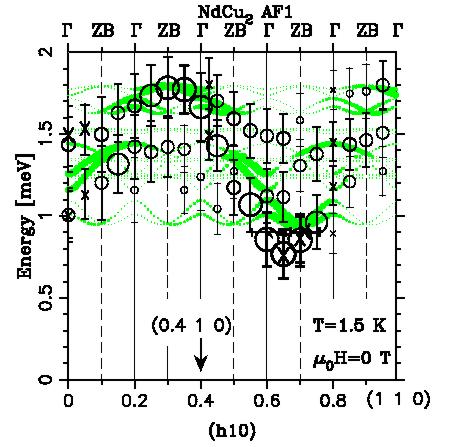
\includegraphics[angle=-0, width=0.6\textwidth]{figsrc/dispAF1.eps}%
\lthtmlpictureZ
\lthtmlcheckvsize\clearpage}

{\newpage\clearpage
\lthtmlpictureA{tex2html_wrap25470}%
\includegraphics[angle=-0, width=0.6\textwidth]{figsrc/animationAF1.eps}%
\lthtmlpictureZ
\lthtmlcheckvsize\clearpage}

\stepcounter{subsection}
{\newpage\clearpage
\lthtmlinlinemathA{tex2html_wrap_inline17364}%
$\hat \mathbf M(\mathbf Q)$%
\lthtmlinlinemathZ
\lthtmlcheckvsize\clearpage}

{\newpage\clearpage
\lthtmlinlinemathA{tex2html_wrap_inline17366}%
$\hat \mathbf M(\mathbf Q)=\hat \mathbf M_S(\mathbf Q)+\hat \mathbf M_L(\mathbf Q)$%
\lthtmlinlinemathZ
\lthtmlcheckvsize\clearpage}

{\newpage\clearpage
\lthtmlinlinemathA{tex2html_wrap_inline17368}%
$\hat \mathcal Q_{\alpha} \equiv -\hat M_{\alpha}(\mathbf Q)/(2\mu_B)$%
\lthtmlinlinemathZ
\lthtmlcheckvsize\clearpage}

{\newpage\clearpage
\lthtmlinlinemathA{tex2html_wrap_inline17370}%
$\alpha=x,y,z$%
\lthtmlinlinemathZ
\lthtmlcheckvsize\clearpage}

{\newpage\clearpage
\lthtmldisplayA{displaymath15736}%
\begin{displaymath}
\frac{d^2\sigma}{d\Omega dE'}=\frac{k'}{k}\left( \frac{m_n}{2\pi \hbar^2}  \right)^2
\sum_{if,s_n} P_{s_n} P_i \left | \langle s_n|\langle i|H_{int}(\mathbf Q)|f\rangle|s_n'\rangle \right |^2 \delta(\hbar \omega+E_i-E_f)
\end{displaymath}%
\lthtmldisplayZ
\lthtmlcheckvsize\clearpage}

{\newpage\clearpage
\lthtmlinlinemathA{tex2html_wrap_inline17380}%
$|s_n\rangle$%
\lthtmlinlinemathZ
\lthtmlcheckvsize\clearpage}

{\newpage\clearpage
\lthtmlinlinemathA{tex2html_wrap_inline17382}%
$|s_n'\rangle$%
\lthtmlinlinemathZ
\lthtmlcheckvsize\clearpage}

{\newpage\clearpage
\lthtmlinlinemathA{tex2html_wrap_inline17384}%
$P_{s_n}$%
\lthtmlinlinemathZ
\lthtmlcheckvsize\clearpage}

{\newpage\clearpage
\lthtmlinlinemathA{tex2html_wrap_inline17386}%
$|s_n>$%
\lthtmlinlinemathZ
\lthtmlcheckvsize\clearpage}

{\newpage\clearpage
\lthtmlinlinemathA{tex2html_wrap_inline17390}%
$|f\rangle$%
\lthtmlinlinemathZ
\lthtmlcheckvsize\clearpage}

{\newpage\clearpage
\lthtmlinlinemathA{tex2html_wrap_inline17392}%
$E_i$%
\lthtmlinlinemathZ
\lthtmlcheckvsize\clearpage}

{\newpage\clearpage
\lthtmlinlinemathA{tex2html_wrap_inline17394}%
$E_f$%
\lthtmlinlinemathZ
\lthtmlcheckvsize\clearpage}

{\newpage\clearpage
\lthtmlinlinemathA{tex2html_wrap_inline17396}%
$P_i$%
\lthtmlinlinemathZ
\lthtmlcheckvsize\clearpage}

{\newpage\clearpage
\lthtmlinlinemathA{tex2html_wrap_inline17400}%
$H_{int}(\mathbf Q)$%
\lthtmlinlinemathZ
\lthtmlcheckvsize\clearpage}

{\newpage\clearpage
\lthtmldisplayA{displaymath15750}%
\begin{displaymath}
H_{int}(\mathbf Q)=\hat \beta (\mathbf Q) + \hat {\mathbf s}_n \cdot \hat {\boldsymbol \alpha } (\mathbf Q)
\end{displaymath}%
\lthtmldisplayZ
\lthtmlcheckvsize\clearpage}

{\newpage\clearpage
\lthtmlinlinemathA{tex2html_wrap_inline17402}%
$\hat \beta$%
\lthtmlinlinemathZ
\lthtmlcheckvsize\clearpage}

{\newpage\clearpage
\lthtmlinlinemathA{tex2html_wrap_inline17404}%
$\hat {\boldsymbol \alpha }$%
\lthtmlinlinemathZ
\lthtmlcheckvsize\clearpage}

{\newpage\clearpage
\lthtmlinlinemathA{tex2html_wrap_inline17406}%
$\hat \beta^{\dagger} \dots \hat \beta$%
\lthtmlinlinemathZ
\lthtmlcheckvsize\clearpage}

{\newpage\clearpage
\lthtmlinlinemathA{tex2html_wrap_inline17408}%
$\hat \alpha^{\dagger} \dots \hat \alpha$%
\lthtmlinlinemathZ
\lthtmlcheckvsize\clearpage}

{\newpage\clearpage
\lthtmlinlinemathA{tex2html_wrap_inline17410}%
$\alpha^{\dagger} \dots \beta$%
\lthtmlinlinemathZ
\lthtmlcheckvsize\clearpage}

{\newpage\clearpage
\lthtmlinlinemathA{tex2html_wrap_indisplay25504}%
$\displaystyle \frac{d^2\sigma}{d\Omega dE'}$%
\lthtmlindisplaymathZ
\lthtmlcheckvsize\clearpage}

{\newpage\clearpage
\lthtmlinlinemathA{tex2html_wrap_indisplay25506}%
$\displaystyle N\frac{k'}{k}S_{\rm nuc}(\mathbf Q,\omega) +
N\frac{k'}{k}
Tr\{S_{\rm mag\perp}(\mathbf Q,\omega)\}$%
\lthtmlindisplaymathZ
\lthtmlcheckvsize\clearpage}

{\newpage\clearpage
\lthtmlinlinemathA{tex2html_wrap_inline17418}%
$\hbar \omega=E-E'$%
\lthtmlinlinemathZ
\lthtmlcheckvsize\clearpage}

{\newpage\clearpage
\lthtmlinlinemathA{tex2html_wrap_inline17422}%
$S_{\rm mag}$%
\lthtmlinlinemathZ
\lthtmlcheckvsize\clearpage}

{\newpage\clearpage
\lthtmlinlinemathA{tex2html_wrap_inline17424}%
$S_{\rm nuc}$%
\lthtmlinlinemathZ
\lthtmlcheckvsize\clearpage}

\stepcounter{subsubsection}
{\newpage\clearpage
\lthtmlinlinemathA{tex2html_wrap_indisplay25522}%
$\displaystyle S_{\rm nuc}^{\rm inel}(\mathbf Q,\omega)$%
\lthtmlindisplaymathZ
\lthtmlcheckvsize\clearpage}

{\newpage\clearpage
\lthtmlinlinemathA{tex2html_wrap_indisplay25524}%
$\displaystyle \frac{1}{2\pi\hbar}\int_{-\infty}^{+\infty}dt e^{i\omega t}
\frac{1}{N}\sum_{nn'} b_n b_{n'} e^{-W_n(Q)- W_{n'}(Q)}$%
\lthtmlindisplaymathZ
\lthtmlcheckvsize\clearpage}

{\newpage\clearpage
\lthtmlinlinemathA{tex2html_wrap_indisplay25525}%
$\textstyle \times$%
\lthtmlindisplaymathZ
\lthtmlcheckvsize\clearpage}

{\newpage\clearpage
\lthtmlinlinemathA{tex2html_wrap_indisplay25526}%
$\displaystyle e^{-i\mathbf Q \cdot (\mathbf R_n-\mathbf R_{n'})}
(\langle  \mathbf Q \cdot \hat {\mathbf u}^{n}(t)  {\mathbf Q} \cdot \hat{\mathbf u}^{n'}(0) \rangle_{T,H}$%
\lthtmlindisplaymathZ
\lthtmlcheckvsize\clearpage}

{\newpage\clearpage
\lthtmlinlinemathA{tex2html_wrap_inline17428}%
$\hat {\mathbf u}$%
\lthtmlinlinemathZ
\lthtmlcheckvsize\clearpage}

{\newpage\clearpage
\lthtmlinlinemathA{tex2html_wrap_inline17432}%
$n=(\ensuremath{\boldsymbol\ell},s)$%
\lthtmlinlinemathZ
\lthtmlcheckvsize\clearpage}

{\newpage\clearpage
\lthtmlinlinemathA{tex2html_wrap_inline17434}%
$\mathbf Q \cdot \hat \mathbf u$%
\lthtmlinlinemathZ
\lthtmlcheckvsize\clearpage}

{\newpage\clearpage
\lthtmlinlinemathA{tex2html_wrap_inline17436}%
$\mathcal O \leftrightarrow b_s   e^{-W_s(Q)} \mathbf Q \cdot\hat \mathbf u^s$%
\lthtmlinlinemathZ
\lthtmlcheckvsize\clearpage}

{\newpage\clearpage
\lthtmlinlinemathA{tex2html_wrap_indisplay25536}%
$\displaystyle \sum_{ss'}
\frac{{\Sigma^{ss'}}({\mathbf Q},\omega)}{2\pi \hbar N_b}$%
\lthtmlindisplaymathZ
\lthtmlcheckvsize\clearpage}

{\newpage\clearpage
\lthtmlinlinemathA{tex2html_wrap_inline17438}%
$W_s(Q)$%
\lthtmlinlinemathZ
\lthtmlcheckvsize\clearpage}

{\newpage\clearpage
\lthtmlinlinemathA{tex2html_wrap_indisplay25543}%
$\displaystyle \sum_{r,ss'}
\frac{(\sqrt{\Gamma_{\rm nuc}^s(\mathbf Q)})^\ast\sqrt{\Gamma_{\rm nuc}^{s'}(\mathbf Q)}}
{N_b(1-e^{-\hbar{\omega^r}(\mathbf Q)/kT})} \times$%
\lthtmlindisplaymathZ
\lthtmlcheckvsize\clearpage}

{\newpage\clearpage
\lthtmlinlinemathA{tex2html_wrap_indisplay25544}%
$\displaystyle \times \mathcal V^s_{{\rm nuc},\alpha1}(\mathbf Q)
{ \mathcal T^{sr}}(\mathbf Q)\hbar {\omega^r}(\mathbf Q)
\delta(\hbar {\omega^r}(\mathbf Q) -
\hbar \omega) {\mathcal T^{rs'\dag }}(\mathbf Q)
\mathcal V^{s'\dag }_{{\rm nuc},1\beta}(\mathbf Q)$%
\lthtmlindisplaymathZ
\lthtmlcheckvsize\clearpage}

{\newpage\clearpage
\lthtmlinlinemathA{tex2html_wrap_inline17450}%
$I_{\rm nuc}$%
\lthtmlinlinemathZ
\lthtmlcheckvsize\clearpage}

\stepcounter{subsubsection}
{\newpage\clearpage
\lthtmlinlinemathA{tex2html_wrap_indisplay25551}%
$\displaystyle S_{\rm mag\perp}^{\rm inel,\alpha\beta}(\mathbf Q,\omega)$%
\lthtmlindisplaymathZ
\lthtmlcheckvsize\clearpage}

{\newpage\clearpage
\lthtmlinlinemathA{tex2html_wrap_indisplay25553}%
$\displaystyle \left( \frac{ \gamma r_0}{2 \mu_B}  \right)^2
\frac{1}{2\pi\hbar}\int_{-\infty}^{+\infty}dt e^{i\omega t}
\frac{1}{N}\sum_{nn'} e^{-W_n(Q)- W_{n'}(Q)}$%
\lthtmlindisplaymathZ
\lthtmlcheckvsize\clearpage}

{\newpage\clearpage
\lthtmlinlinemathA{tex2html_wrap_indisplay25555}%
$\displaystyle e^{-i\mathbf Q \cdot (\mathbf R_n-\mathbf R_{n'})}   (\langle \hat M_{\perp\alpha}^{n \dag }(t,\mathbf Q)  \hat M_{\perp\beta}^{n'}(0,\mathbf Q) \rangle_{T,H}
- \langle \hat M^{n \dag }_{\perp\alpha}(\mathbf Q)\rangle_{T,H} \langle \hat M^{n'}_{\perp\beta}(\mathbf Q) \rangle_{T,H})$%
\lthtmlindisplaymathZ
\lthtmlcheckvsize\clearpage}

{\newpage\clearpage
\lthtmlinlinemathA{tex2html_wrap_inline17452}%
$4\pi (\gamma r_0)^2=4\pi\left(\frac{\hbar \gamma e^2}{mc^2}\right)^2
=3.65$%
\lthtmlinlinemathZ
\lthtmlcheckvsize\clearpage}

{\newpage\clearpage
\lthtmlinlinemathA{tex2html_wrap_inline17458}%
$\hat \mathbf M_{\perp}(\mathbf Q)=\hat \mathbf M(\mathbf Q)-\mathbf Q (\hat \mathbf M_{\perp}(\mathbf Q) \cdot \mathbf Q)/Q^2$%
\lthtmlinlinemathZ
\lthtmlcheckvsize\clearpage}

{\newpage\clearpage
\lthtmlinlinemathA{tex2html_wrap_inline17460}%
$\mathcal O \leftrightarrow \frac{ \gamma r_0}{2 \mu_B}  e^{-W(Q)} \hat \mathbf M_{\perp}(\mathbf Q)$%
\lthtmlinlinemathZ
\lthtmlcheckvsize\clearpage}

{\newpage\clearpage
\lthtmldisplayA{displaymath15884}%
\begin{displaymath}
S_{\rm mag\perp}^{\rm inel,\alpha\beta}(\mathbf Q,\omega)=
\sum_{ss'} 
  \frac{{\Sigma^{ss'}_{\alpha\beta}}({\mathbf Q},\omega)}{2\pi \hbar N_b} 
\end{displaymath}%
\lthtmldisplayZ
\lthtmlcheckvsize\clearpage}

{\newpage\clearpage
\lthtmlinlinemathA{tex2html_wrap_indisplay25570}%
$\displaystyle \sum_{r,ss'}
\frac{(\sqrt{\Gamma_{\rm mag}^s(\mathbf Q)})^\ast\sqrt{\Gamma_{\rm mag}^{s'}(\mathbf Q)} }
{N_b(1-e^{-\hbar{\omega^r}(\mathbf Q)/kT})} \times$%
\lthtmlindisplaymathZ
\lthtmlcheckvsize\clearpage}

{\newpage\clearpage
\lthtmlinlinemathA{tex2html_wrap_indisplay25571}%
$\displaystyle \times \mathcal V^s_{{\rm mag},\alpha1}(\mathbf Q)
{ \mathcal T^{sr}}(\mathbf Q)\hbar {\omega^r}(\mathbf Q)
\delta(\hbar {\omega^r}(\mathbf Q) -
\hbar \omega) {\mathcal T^{rs'\dag }}(\mathbf Q)
\mathcal V^{s'\dag }_{{\rm mag},1\beta}(\mathbf Q)$%
\lthtmlindisplaymathZ
\lthtmlcheckvsize\clearpage}

{\newpage\clearpage
\lthtmlinlinemathA{tex2html_wrap_inline17476}%
$S_{\rm mag}^{\rm inel,\alpha\beta}(\mathbf Q,\omega)$%
\lthtmlinlinemathZ
\lthtmlcheckvsize\clearpage}

{\newpage\clearpage
\lthtmlinlinemathA{tex2html_wrap_inline17478}%
$\alpha,\beta$%
\lthtmlinlinemathZ
\lthtmlcheckvsize\clearpage}

{\newpage\clearpage
\lthtmlinlinemathA{tex2html_wrap_inline17490}%
$\mathbf u||\mathbf Q=\mathbf k- \mathbf k'$%
\lthtmlinlinemathZ
\lthtmlcheckvsize\clearpage}

{\newpage\clearpage
\lthtmlinlinemathA{tex2html_wrap_inline17492}%
$\mathbf w$%
\lthtmlinlinemathZ
\lthtmlcheckvsize\clearpage}

{\newpage\clearpage
\lthtmlinlinemathA{tex2html_wrap_inline17494}%
$\mathbf v$%
\lthtmlinlinemathZ
\lthtmlcheckvsize\clearpage}

{\newpage\clearpage
\lthtmlinlinemathA{tex2html_wrap_inline17508}%
$\hat \mathbf M_{\perp}(\mathbf Q)$%
\lthtmlinlinemathZ
\lthtmlcheckvsize\clearpage}

{\newpage\clearpage
\lthtmlinlinemathA{tex2html_wrap_inline17512}%
$\mathcal O \leftrightarrow \hat \mathbf M_{\perp}(\mathbf Q)$%
\lthtmlinlinemathZ
\lthtmlcheckvsize\clearpage}

\stepcounter{subsection}
{\newpage\clearpage
\lthtmlinlinemathA{tex2html_wrap_inline17516}%
$1/Q$%
\lthtmlinlinemathZ
\lthtmlcheckvsize\clearpage}

{\newpage\clearpage
\lthtmldisplayA{displaymath15929}%
\begin{displaymath}
\hat M^{n}_{\alpha}(\mathbf Q) \approx -\mu_B[F^n_S(Q) g_S \hat S^{n}_{\alpha} + F^n_L(Q) g_L \hat L^{n}_{\alpha}]
\end{displaymath}%
\lthtmldisplayZ
\lthtmlcheckvsize\clearpage}

{\newpage\clearpage
\lthtmlinlinemathA{tex2html_wrap_inline17518}%
$g$%
\lthtmlinlinemathZ
\lthtmlcheckvsize\clearpage}

{\newpage\clearpage
\lthtmlinlinemathA{tex2html_wrap_inline17520}%
$g_S \approx 2$%
\lthtmlinlinemathZ
\lthtmlcheckvsize\clearpage}

{\newpage\clearpage
\lthtmlinlinemathA{tex2html_wrap_inline17522}%
$g_L=1$%
\lthtmlinlinemathZ
\lthtmlcheckvsize\clearpage}

{\newpage\clearpage
\lthtmlinlinemathA{tex2html_wrap_inline17524}%
$F_S(Q)=\langle j_0 (Q) \rangle$%
\lthtmlinlinemathZ
\lthtmlcheckvsize\clearpage}

{\newpage\clearpage
\lthtmlinlinemathA{tex2html_wrap_inline17526}%
$F_L(Q)=\langle j_0 (Q) \rangle + \langle j_2 (Q) \rangle$%
\lthtmlinlinemathZ
\lthtmlcheckvsize\clearpage}

{\newpage\clearpage
\lthtmlinlinemathA{tex2html_wrap_inline17530}%
$\hat S^{n}_{\alpha}$%
\lthtmlinlinemathZ
\lthtmlcheckvsize\clearpage}

{\newpage\clearpage
\lthtmlinlinemathA{tex2html_wrap_inline17532}%
$\hat L^{n}_{\alpha}$%
\lthtmlinlinemathZ
\lthtmlcheckvsize\clearpage}

{\newpage\clearpage
\lthtmlinlinemathA{tex2html_wrap_inline17534}%
$\hat M^{n}_{\alpha}(\mathbf Q) \leftrightarrow -\mu_B
\{ F^n_S(Q) g_S \hat S^{n}_{\alpha} + F^n_L(Q) g_L \hat L^{n}_{\alpha} \}$%
\lthtmlinlinemathZ
\lthtmlcheckvsize\clearpage}

{\newpage\clearpage
\lthtmlinlinemathA{tex2html_wrap_inline17536}%
$\hat M^{n}_{\alpha}(\mathbf Q) \leftrightarrow -\mu_B
F^n_S(Q) g_S \hat S^{n}_{\alpha}$%
\lthtmlinlinemathZ
\lthtmlcheckvsize\clearpage}

{\newpage\clearpage
\lthtmlinlinemathA{tex2html_wrap_inline17542}%
$\hat M^{n}_{\alpha}(\mathbf Q) \leftrightarrow -\mu_B
 g_J F^n(Q) \hat J_{\alpha}^n$%
\lthtmlinlinemathZ
\lthtmlcheckvsize\clearpage}

{\newpage\clearpage
\lthtmlinlinemathA{tex2html_wrap_inline17546}%
$\hat M^{n}_{\alpha} \approx -\mu_B g_J F^n(Q)  \hat J_{\alpha}^n $%
\lthtmlinlinemathZ
\lthtmlcheckvsize\clearpage}

{\newpage\clearpage
\lthtmlinlinemathA{tex2html_wrap_inline17548}%
$F(Q)=\langle j_0 (Q) \rangle + \frac{2-g_J}{g_J}\langle j_2 (Q) \rangle $%
\lthtmlinlinemathZ
\lthtmlcheckvsize\clearpage}

{\newpage\clearpage
\lthtmlinlinemathA{tex2html_wrap_indisplay25619}%
$\displaystyle S_{\rm mag}^{\rm inel,\alpha\beta}(\mathbf Q,\omega)$%
\lthtmlindisplaymathZ
\lthtmlcheckvsize\clearpage}

{\newpage\clearpage
\lthtmlinlinemathA{tex2html_wrap_indisplay25623}%
$\displaystyle e^{-i\mathbf Q \cdot (\mathbf R_n-\mathbf R_{n'})}   (\langle \hat M_{\alpha}^{n \dag }(t,\mathbf Q)  \hat M_{\beta}^{n'}(0,\mathbf Q) \rangle_{T,H}
- \langle \hat M^{n \dag }_{\alpha}(\mathbf Q)\rangle_{T,H} \langle \hat M^{n'}_{\beta}(\mathbf Q) \rangle_{T,H})$%
\lthtmlindisplaymathZ
\lthtmlcheckvsize\clearpage}

\stepcounter{section}
{\newpage\clearpage
\lthtmldisplayA{displaymath18557}%
\begin{displaymath}
\chi_{\alpha\beta}(t)={i\over \hbar} \Theta(t)\langle [J^\dagger_\alpha(t), J_\beta(0)]\rangle 
\end{displaymath}%
\lthtmldisplayZ
\lthtmlcheckvsize\clearpage}

{\newpage\clearpage
\lthtmldisplayA{displaymath18559}%
\begin{displaymath}
\chi_{\alpha,\beta}(z)=\int_{-\infty}^{+\infty} dt e^{izt}\chi_{\alpha\beta}(t), \quad z=\omega
+i\delta 
\end{displaymath}%
\lthtmldisplayZ
\lthtmlcheckvsize\clearpage}

{\newpage\clearpage
\lthtmldisplayA{displaymath18561}%
\begin{displaymath}
{d^2\sigma \over d\Omega d E'}=  {k' \over
k}({r_0\over 2}g_J F(Q))^2{1\over \pi }
\sum_{\alpha\beta}(\delta_{\alpha\beta} 
- \tilde Q_\alpha \tilde Q_\beta)
{ \chi{"}_{\alpha,\beta}(\omega)\over 1-e^{-\beta \hbar \omega}} 
\end{displaymath}%
\lthtmldisplayZ
\lthtmlcheckvsize\clearpage}

{\newpage\clearpage
\lthtmlinlinemathA{tex2html_wrap_inline18567}%
$\vec Q = \vec k - \vec k'$%
\lthtmlinlinemathZ
\lthtmlcheckvsize\clearpage}

{\newpage\clearpage
\lthtmlinlinemathA{tex2html_wrap_inline18569}%
$\tilde Q = \vec Q/\vert\vec Q\vert$%
\lthtmlinlinemathZ
\lthtmlcheckvsize\clearpage}

{\newpage\clearpage
\lthtmlinlinemathA{tex2html_wrap_inline18571}%
$r_0= -0.54 \cdot 10^{-12}$%
\lthtmlinlinemathZ
\lthtmlcheckvsize\clearpage}

{\newpage\clearpage
\lthtmlinlinemathA{tex2html_wrap_inline18575}%
$F(Q)$%
\lthtmlinlinemathZ
\lthtmlcheckvsize\clearpage}

{\newpage\clearpage
\lthtmldisplayA{displaymath18577}%
\begin{displaymath}
\chi_{i,k}(t)=i \Theta(t) \langle [A_i^\dagger(t),A_k(0)]\rangle
\end{displaymath}%
\lthtmldisplayZ
\lthtmlcheckvsize\clearpage}

{\newpage\clearpage
\lthtmlinlinemathA{tex2html_wrap_inline18579}%
$A(t)$%
\lthtmlinlinemathZ
\lthtmlcheckvsize\clearpage}

{\newpage\clearpage
\lthtmldisplayA{displaymath18581}%
\begin{displaymath}
A(t)= \exp(iHt)A\exp(-iHt)
\end{displaymath}%
\lthtmldisplayZ
\lthtmlcheckvsize\clearpage}

{\newpage\clearpage
\lthtmlinlinemathA{tex2html_wrap_inline18583}%
${\cal L}A = [H,A]$%
\lthtmlinlinemathZ
\lthtmlcheckvsize\clearpage}

{\newpage\clearpage
\lthtmldisplayA{displaymath18585}%
\begin{displaymath}
A(t)= \exp(i{\cal L}t) A
\end{displaymath}%
\lthtmldisplayZ
\lthtmlcheckvsize\clearpage}

{\newpage\clearpage
\lthtmlinlinemathA{tex2html_wrap_inline18587}%
$\chi_{i,k}$%
\lthtmlinlinemathZ
\lthtmlcheckvsize\clearpage}

{\newpage\clearpage
\lthtmlinlinemathA{tex2html_wrap_inline18589}%
$A_i, A_k$%
\lthtmlinlinemathZ
\lthtmlcheckvsize\clearpage}

{\newpage\clearpage
\lthtmldisplayA{displaymath18593}%
\begin{displaymath}
\chi_{i,k}(z)=i\int_0^\infty dt e^{izt} \langle [A_i^\dagger(t),A_k(0)]\rangle
\end{displaymath}%
\lthtmldisplayZ
\lthtmlcheckvsize\clearpage}

{\newpage\clearpage
\lthtmldisplayA{displaymath18595}%
\begin{displaymath}
\chi_{i,k}(t)=i \Theta(t) \langle [A_i^\dagger,A_k\exp^{-i{\cal L}t}\rangle
\end{displaymath}%
\lthtmldisplayZ
\lthtmlcheckvsize\clearpage}

{\newpage\clearpage
\lthtmldisplayA{displaymath18597}%
\begin{displaymath}
\chi_{i,k}(z)= -\langle [A_i^\dagger,{1\over {z-\cal
L}}A_k(0)]\rangle
\end{displaymath}%
\lthtmldisplayZ
\lthtmlcheckvsize\clearpage}

{\newpage\clearpage
\lthtmldisplayA{displaymath18599}%
\begin{displaymath}
\chi_{i,k}(0) = \int_0^\beta d \lambda \langle e^{\lambda H}
A_i^\dagger e^{-\lambda H}  A_k\rangle
 = \int_0^\beta d \lambda \langle (e^{\lambda {\cal L}}
A_i^\dagger)   A_k\rangle
\end{displaymath}%
\lthtmldisplayZ
\lthtmlcheckvsize\clearpage}

{\newpage\clearpage
\lthtmldisplayA{displaymath18601}%
\begin{displaymath}
(A_i \vert A_k) =  {1\over \beta }\int_0^\beta d\lambda \langle
(e^{\lambda{\cal L}}A_i^\dagger)A_k\rangle ={1\over \beta} \chi_{ik}(0)
\end{displaymath}%
\lthtmldisplayZ
\lthtmlcheckvsize\clearpage}

{\newpage\clearpage
\lthtmldisplayA{displaymath18603}%
\begin{displaymath}
({\cal L}A_i\vert A_k)=(A_i\vert {\cal L}A_k)={1\over \beta}\langle
[A_i^\dagger,A_k]\rangle
\end{displaymath}%
\lthtmldisplayZ
\lthtmlcheckvsize\clearpage}

{\newpage\clearpage
\lthtmldisplayA{displaymath18605}%
\begin{displaymath}
\chi_{i,k}(z)= -\beta (A_i\vert {{\cal L}\over {z-\cal L}} A_k)
\end{displaymath}%
\lthtmldisplayZ
\lthtmlcheckvsize\clearpage}

{\newpage\clearpage
\lthtmldisplayA{displaymath18607}%
\begin{displaymath}
\chi_{ik}(z)=\chi_{ik}(0)-z\beta (A_i\vert {1\over {z-\cal L}}A_k)  
\end{displaymath}%
\lthtmldisplayZ
\lthtmlcheckvsize\clearpage}

{\newpage\clearpage
\lthtmldisplayA{displaymath18609}%
\begin{displaymath}
\Phi_{ik}(z)=(A_i \vert {1 \over {z-\cal L}}A_k)
\end{displaymath}%
\lthtmldisplayZ
\lthtmlcheckvsize\clearpage}

{\newpage\clearpage
\lthtmldisplayA{displaymath18611}%
\begin{displaymath}
H=H_{cf}+H_{el}+H_{el,cf} 
\end{displaymath}%
\lthtmldisplayZ
\lthtmlcheckvsize\clearpage}

{\newpage\clearpage
\lthtmldisplayA{displaymath18613}%
\begin{displaymath} 
H_{cf}= \sum_n E_n K_{nn}, \quad K_{nm}= \vert n\rangle \langle m\vert
\end{displaymath}%
\lthtmldisplayZ
\lthtmlcheckvsize\clearpage}

{\newpage\clearpage
\lthtmlinlinemathA{tex2html_wrap_inline18615}%
$\vert n\rangle$%
\lthtmlinlinemathZ
\lthtmlcheckvsize\clearpage}

{\newpage\clearpage
\lthtmldisplayA{displaymath18617}%
\begin{displaymath}
H_{el}=\sum_{k\alpha}\epsilon_kc^\dagger_{k\alpha}c_{k\alpha}
\end{displaymath}%
\lthtmldisplayZ
\lthtmlcheckvsize\clearpage}

{\newpage\clearpage
\lthtmldisplayA{displaymath18619}%
\begin{displaymath}
H_{el,cf}= - J_{ex}\vec J \cdot \vec \sigma, \quad \vec \sigma = \sum_{k\alpha
Q\beta}\vec \sigma_{\alpha\beta}c^\dagger_{k\alpha}c_{k+Q\beta}, \quad \vec
J=\sum_{n,m}\vec J_{n,m}K_{nm}.
\end{displaymath}%
\lthtmldisplayZ
\lthtmlcheckvsize\clearpage}

{\newpage\clearpage
\lthtmlinlinemathA{tex2html_wrap_inline18621}%
$E_n$%
\lthtmlinlinemathZ
\lthtmlcheckvsize\clearpage}

{\newpage\clearpage
\lthtmldisplayA{displaymath18625}%
\begin{displaymath}
A_\mu= K_{\mu}
\end{displaymath}%
\lthtmldisplayZ
\lthtmlcheckvsize\clearpage}

{\newpage\clearpage
\lthtmlinlinemathA{tex2html_wrap_inline18627}%
$\mu= [nm]$%
\lthtmlinlinemathZ
\lthtmlcheckvsize\clearpage}

{\newpage\clearpage
\lthtmldisplayA{displaymath18633}%
\begin{displaymath}
{\cal L}A_\mu = (E_n-E_m)A_\mu
\end{displaymath}%
\lthtmldisplayZ
\lthtmlcheckvsize\clearpage}

{\newpage\clearpage
\lthtmldisplayA{displaymath18635}%
\begin{displaymath} 
\chi_{\alpha \beta}   
\end{displaymath}%
\lthtmldisplayZ
\lthtmlcheckvsize\clearpage}

{\newpage\clearpage
\lthtmlinlinemathA{tex2html_wrap_inline18637}%
$A$%
\lthtmlinlinemathZ
\lthtmlcheckvsize\clearpage}

{\newpage\clearpage
\lthtmlinlinemathA{tex2html_wrap_inline18639}%
$A_i$%
\lthtmlinlinemathZ
\lthtmlcheckvsize\clearpage}

{\newpage\clearpage
\lthtmldisplayA{displaymath18641}%
\begin{displaymath}
{\cal P} A= \sum_{\nu \mu}A_\nu P^{-1}_{\nu \mu}(A_\mu\vert A) \quad
P_{\nu\mu}=(A_\nu\vert A_\mu)
\end{displaymath}%
\lthtmldisplayZ
\lthtmlcheckvsize\clearpage}

{\newpage\clearpage
\lthtmlinlinemathA{tex2html_wrap_inline18643}%
$ P^{-1}_{\nu \mu}=[P^{-1}]_{\nu \mu}$%
\lthtmlinlinemathZ
\lthtmlcheckvsize\clearpage}

{\newpage\clearpage
\lthtmlinlinemathA{tex2html_wrap_inline18645}%
${\nu\mu}$%
\lthtmlinlinemathZ
\lthtmlcheckvsize\clearpage}

{\newpage\clearpage
\lthtmlinlinemathA{tex2html_wrap_inline18647}%
$P$%
\lthtmlinlinemathZ
\lthtmlcheckvsize\clearpage}

{\newpage\clearpage
\lthtmldisplayA{displaymath18649}%
\begin{displaymath}
{\cal F}(z)= {1\over {z-\cal L}}, \quad ({z-\cal L}){\cal F}(z)=1 
\end{displaymath}%
\lthtmldisplayZ
\lthtmlcheckvsize\clearpage}

{\newpage\clearpage
\lthtmldisplayA{displaymath18651}%
\begin{displaymath}
({\cal P}(z-{\cal P}{\cal L}{\cal P} - {\cal P} {\cal M}(z) {\cal P}){\cal P} {\cal
F}(z) {\cal P}= {\cal P}
\end{displaymath}%
\lthtmldisplayZ
\lthtmlcheckvsize\clearpage}

{\newpage\clearpage
\lthtmldisplayA{displaymath18653}%
\begin{displaymath}
{\cal M}(z)={\cal PLQ}{1\over z-{\cal QLQ} }{\cal QLP}
\end{displaymath}%
\lthtmldisplayZ
\lthtmlcheckvsize\clearpage}

{\newpage\clearpage
\lthtmlinlinemathA{tex2html_wrap_inline18655}%
${\cal Q}=1-{\cal P}$%
\lthtmlinlinemathZ
\lthtmlcheckvsize\clearpage}

{\newpage\clearpage
\lthtmldisplayA{displaymath18657}%
\begin{displaymath}
\Phi_{\nu\mu}(z)= (A_\nu\vert {1\over z-{\cal L}} A_\mu)
\end{displaymath}%
\lthtmldisplayZ
\lthtmlcheckvsize\clearpage}

{\newpage\clearpage
\lthtmldisplayA{displaymath18659}%
\begin{displaymath}
\sum_\lambda \Bigl(z\delta_{\nu\lambda}-\sum_\kappa\bigl[L_{\nu\kappa}+
M_{\nu\kappa}(z)\bigr]P^{-1}_{\kappa\lambda}\Bigr)\Phi_{\lambda\mu}(z)
=P_{\nu \mu}
\end{displaymath}%
\lthtmldisplayZ
\lthtmlcheckvsize\clearpage}

{\newpage\clearpage
\lthtmldisplayA{displaymath18661}%
\begin{displaymath}
L_{\nu\mu}=(A_\nu\vert {\cal L}A_\mu)
\end{displaymath}%
\lthtmldisplayZ
\lthtmlcheckvsize\clearpage}

{\newpage\clearpage
\lthtmldisplayA{displaymath18663}%
\begin{displaymath}
M_{\nu\mu}(z)=(A_\nu\vert{\cal M}(z)A_\mu)
\end{displaymath}%
\lthtmldisplayZ
\lthtmlcheckvsize\clearpage}

{\newpage\clearpage
\lthtmldisplayA{displaymath18665}%
\begin{displaymath}
J^\alpha=\sum_{n_1,n_2}J^\alpha_{n_2,n_1}K_{n_2,n_1}=\sum_\nu J^\alpha_\nu A_\nu, 
\quad 
A_\nu= K_{n_1n_2}   
\end{displaymath}%
\lthtmldisplayZ
\lthtmlcheckvsize\clearpage}

{\newpage\clearpage
\lthtmlinlinemathA{tex2html_wrap_inline18669}%
$n_2 \gets n_1$%
\lthtmlinlinemathZ
\lthtmlcheckvsize\clearpage}

{\newpage\clearpage
\lthtmlinlinemathA{tex2html_wrap_inline18671}%
$\vert n_2\rangle\langle n_1\vert$%
\lthtmlinlinemathZ
\lthtmlcheckvsize\clearpage}

{\newpage\clearpage
\lthtmldisplayA{displaymath18673}%
\begin{displaymath}
{\cal L}A_\nu = (E_{n_2}-E_{n_1)}A_\nu
\end{displaymath}%
\lthtmldisplayZ
\lthtmlcheckvsize\clearpage}

{\newpage\clearpage
\lthtmldisplayA{displaymath18675}%
\begin{displaymath}
P_{\nu\mu}=(A_\nu\vert A_\mu)\simeq\delta_{\nu
\mu}P_\nu, \quad P_\nu=(A_\nu\vert
A_\nu)={p(n_1)-p(n_2)\over \beta (E_{n2}-E_{n_1})}
\end{displaymath}%
\lthtmldisplayZ
\lthtmlcheckvsize\clearpage}

{\newpage\clearpage
\lthtmlinlinemathA{tex2html_wrap_inline18677}%
$p(n)=\exp(-\beta E_n)/Z$%
\lthtmlinlinemathZ
\lthtmlcheckvsize\clearpage}

{\newpage\clearpage
\lthtmldisplayA{displaymath18679}%
\begin{displaymath}
L_{\nu\mu}=\delta_{\nu\mu}(A_\nu\vert A_\nu) (E_{n_2}-E_{n_1} )
+O(J_{ex}^2)
\end{displaymath}%
\lthtmldisplayZ
\lthtmlcheckvsize\clearpage}

{\newpage\clearpage
\lthtmldisplayA{displaymath18681}%
\begin{displaymath}
\Phi_{\nu\mu}(z)=\bigl[\Omega^{-1}\bigr]_{\nu\mu}(z)
P_\mu, \quad
\Omega_{\nu\mu}(z)=(z-E_\nu)\delta_{\nu\mu} -
M_{\nu\mu}(z)[P^{-1}]_\mu, \quad
E_\nu = E_{n_2}- E_{n_1}
\end{displaymath}%
\lthtmldisplayZ
\lthtmlcheckvsize\clearpage}

{\newpage\clearpage
\lthtmlinlinemathA{tex2html_wrap_inline18683}%
${\cal QL}A_\nu$%
\lthtmlinlinemathZ
\lthtmlcheckvsize\clearpage}

{\newpage\clearpage
\lthtmlinlinemathA{tex2html_wrap_inline18685}%
${\cal L}_{el,cf}A_\nu$%
\lthtmlinlinemathZ
\lthtmlcheckvsize\clearpage}

{\newpage\clearpage
\lthtmldisplayA{displaymath18687}%
\begin{displaymath}
M_{\nu \mu}(z)= ({\cal L}_{el,cf}A_\nu \vert{1\over z- {\cal
L}_0}{\cal L}_{el,cf}A_\mu)=
M_{n_2n_1,m_2m_1}(z)
\end{displaymath}%
\lthtmldisplayZ
\lthtmlcheckvsize\clearpage}

{\newpage\clearpage
\lthtmldisplayA{displaymath18689}%
\begin{displaymath}
M_{n_2n_1,m_2m_1}(z)=({\cal L}_{el,cf} K_{n_2n_1}\vert{1\over z-{\cal
L}_0}{\cal L}_{el,cf} K_{m_2m_1})
\end{displaymath}%
\lthtmldisplayZ
\lthtmlcheckvsize\clearpage}

{\newpage\clearpage
\lthtmldisplayA{displaymath18691}%
\begin{displaymath}
{\cal L}_{el,cf} K_{n_2n_1} = J_{ex}\sum_t \vec \sigma(\vec  J_{n_1t}
K_{n_2t} - \vec
J_{tn_2}K_{tn_1})
\end{displaymath}%
\lthtmldisplayZ
\lthtmlcheckvsize\clearpage}

{\newpage\clearpage
\lthtmldisplayA{displaymath18693}%
\begin{displaymath}
\vec \sigma = \sum_{k\alpha, k+Q\beta}\vec \sigma_{\alpha\beta}
c^\dagger_{k\alpha}c_{k+Q\beta}
\end{displaymath}%
\lthtmldisplayZ
\lthtmlcheckvsize\clearpage}

{\newpage\clearpage
\lthtmldisplayA{displaymath18695}%
\begin{displaymath}
( \sigma^i K_{nm}\vert {1\over z- {\cal L}_0}\sigma^j K_{n'm'})=
\delta_{ij}\delta_{nn'}\delta_{mm'}G_{nm}(z)
\end{displaymath}%
\lthtmldisplayZ
\lthtmlcheckvsize\clearpage}

{\newpage\clearpage
\lthtmldisplayA{displaymath18697}%
\begin{displaymath}
G_{nm}(z)=( \sigma^i K_{nm}\vert {1\over  {z-\cal L}_0}\sigma^i K_{nm})
\end{displaymath}%
\lthtmldisplayZ
\lthtmlcheckvsize\clearpage}

{\newpage\clearpage
\lthtmlinlinemathA{tex2html_wrap_indisplay25697}%
$\displaystyle M_{n_2n_1,m_2m_1}(z)=J_{ex}^2\sum_i\Bigl[$%
\lthtmlindisplaymathZ
\lthtmlcheckvsize\clearpage}

{\newpage\clearpage
\lthtmlinlinemathA{tex2html_wrap_indisplay25698}%
$\textstyle \delta_{n_2m_2}\sum_tJ^i_{m_1t}J^i_{tn_1}G_{n_2t}
+ \delta_{n_1m_1}\sum_tJ^i_{
n_2t}J^i_{tm_2}G_{tn_1}$%
\lthtmlindisplaymathZ
\lthtmlcheckvsize\clearpage}

{\newpage\clearpage
\lthtmlinlinemathA{tex2html_wrap_indisplay25699}%
$\textstyle -J^i_{m_1n_1}J^i_{n_2m_2}G_{n_2m_1}
-J^i_{n_2m_2}J^i_{m_1n_1}G_{m_2n_1}\Bigr]$%
\lthtmlindisplaymathZ
\lthtmlcheckvsize\clearpage}

{\newpage\clearpage
\lthtmlinlinemathA{tex2html_wrap_inline18699}%
$G_{n,m}(z)$%
\lthtmlinlinemathZ
\lthtmlcheckvsize\clearpage}

{\newpage\clearpage
\lthtmldisplayA{displaymath18701}%
\begin{displaymath}
\chi(z)= \chi(0)-\beta z \Phi(z)
\end{displaymath}%
\lthtmldisplayZ
\lthtmlcheckvsize\clearpage}

{\newpage\clearpage
\lthtmlinlinemathA{tex2html_wrap_inline18703}%
$\sigma^i\sigma^i)=2$%
\lthtmlinlinemathZ
\lthtmlcheckvsize\clearpage}

{\newpage\clearpage
\lthtmlinlinemathA{tex2html_wrap_indisplay25704}%
$\displaystyle G_{nm}(z)$%
\lthtmlindisplaymathZ
\lthtmlcheckvsize\clearpage}

{\newpage\clearpage
\lthtmlinlinemathA{tex2html_wrap_indisplay25705}%
$\textstyle = {2\over \beta \omega}\sum_{k,k+Q} \langle \Bigl[K_{mn}
c^\dagger_{k+Q}c_{k},(z - E_n +
E_m  -\epsilon_k+\epsilon_{k+Q})^{-1} K_{nm}
c^\dagger_{k}c_{k+Q}\Bigr]\rangle$%
\lthtmlindisplaymathZ
\lthtmlcheckvsize\clearpage}

{\newpage\clearpage
\lthtmlinlinemathA{tex2html_wrap_indisplay25706}%
$\textstyle =  {2\over \beta \omega
}\sum_{k,Q}(f_{k+Q}(1-f_{k})p_m-f_{k}(1-f_{k+Q})p_n)(
z-E_n+E_m-\epsilon_{k}+\epsilon_{k+Q})^{-1}$%
\lthtmlindisplaymathZ
\lthtmlcheckvsize\clearpage}

{\newpage\clearpage
\lthtmldisplayA{displaymath18705}%
\begin{displaymath}
Im G_{nm}(\omega+i\delta)= - {2\pi \over \beta \omega
}\sum_{k,Q}\Bigl(f_{k+Q}(1-f_{k})p_m-f_{k}(1-f_{k+Q})p_n \Bigr)
 \delta(\omega -E_n+E_m-\epsilon_{k}+\epsilon_{k+Q})
\end{displaymath}%
\lthtmldisplayZ
\lthtmlcheckvsize\clearpage}

{\newpage\clearpage
\lthtmlinlinemathA{tex2html_wrap_inline18707}%
$ \rho=\omega - \omega_{nm}$%
\lthtmlinlinemathZ
\lthtmlcheckvsize\clearpage}

{\newpage\clearpage
\lthtmlinlinemathA{tex2html_wrap_inline18709}%
$\omega_{nm}=E_n-E_m$%
\lthtmlinlinemathZ
\lthtmlcheckvsize\clearpage}

{\newpage\clearpage
\lthtmldisplayA{displaymath18711}%
\begin{displaymath}
Im G_{nm}(\omega+i\delta)= - {2\pi N^2(0)\over \beta \omega} \int d\epsilon  
 (f(\epsilon)(1-f(\epsilon+\rho) p_m
- f(\epsilon+\rho)(1-f(\epsilon))p_n)
\end{displaymath}%
\lthtmldisplayZ
\lthtmlcheckvsize\clearpage}

{\newpage\clearpage
\lthtmlinlinemathA{tex2html_wrap_indisplay25712}%
$\displaystyle \int d\epsilon f(\epsilon)(1-f(\epsilon+\rho)=$%
\lthtmlindisplaymathZ
\lthtmlcheckvsize\clearpage}

{\newpage\clearpage
\lthtmlinlinemathA{tex2html_wrap_indisplay25713}%
$\textstyle \int d\epsilon
\exp(\beta(\epsilon+\rho))/
(1+\exp(\beta\epsilon))(1+\exp(\beta(\epsilon+\rho))$%
\lthtmlindisplaymathZ
\lthtmlcheckvsize\clearpage}

{\newpage\clearpage
\lthtmlinlinemathA{tex2html_wrap_indisplay25714}%
$\displaystyle =$%
\lthtmlindisplaymathZ
\lthtmlcheckvsize\clearpage}

{\newpage\clearpage
\lthtmlinlinemathA{tex2html_wrap_indisplay25715}%
$\textstyle (\omega-\omega_{nm})\exp(\beta(\omega-\omega_{nm}))/
(-1+\exp(\beta(\omega-\omega_{nm})$%
\lthtmlindisplaymathZ
\lthtmlcheckvsize\clearpage}

{\newpage\clearpage
\lthtmlinlinemathA{tex2html_wrap_indisplay25717}%
$\displaystyle \int d\epsilon f(\epsilon+\rho )(1-f(\epsilon)=$%
\lthtmlindisplaymathZ
\lthtmlcheckvsize\clearpage}

{\newpage\clearpage
\lthtmlinlinemathA{tex2html_wrap_indisplay25718}%
$\textstyle \int d\epsilon
\exp(\beta(\epsilon)/
(1+\exp(\beta\epsilon))(1+\exp(\beta(\epsilon+\rho))$%
\lthtmlindisplaymathZ
\lthtmlcheckvsize\clearpage}

{\newpage\clearpage
\lthtmlinlinemathA{tex2html_wrap_indisplay25720}%
$\textstyle (\omega-\omega_{nm})/
(-1+\exp(\beta(\omega-\omega_{nm}))$%
\lthtmlindisplaymathZ
\lthtmlcheckvsize\clearpage}

{\newpage\clearpage
\lthtmldisplayA{displaymath18713}%
\begin{displaymath}
Im G_{nm}=-{2\pi N^2(0)\over \beta \omega}(\omega -\omega_{nm}) {1-\exp(-\beta
\omega)\over
1-\exp[(\omega_{nm}-\omega)\beta]}p_m
\end{displaymath}%
\lthtmldisplayZ
\lthtmlcheckvsize\clearpage}

{\newpage\clearpage
\lthtmldisplayA{displaymath18715}%
\begin{displaymath}
F_{nm}(\omega )= {1\over \beta \omega}(\omega -\omega_{nm}) {1-\exp(-\beta
\omega)\over
1-\exp[(\omega_{nm}-\omega)\beta]}p_m
\end{displaymath}%
\lthtmldisplayZ
\lthtmlcheckvsize\clearpage}

{\newpage\clearpage
\lthtmldisplayA{displaymath18717}%
\begin{displaymath}
F_{nm}(\omega )= {\sqrt{p_np_m}\over \beta}{(\omega -\omega_{nm})\over
\omega} {\exp(\beta \omega)/2) - \exp(-\beta \omega)/2)\over
\exp(\beta (\omega-\omega_{nm})/2) - \exp(-\beta (\omega -\omega_{nm})/2)}
\end{displaymath}%
\lthtmldisplayZ
\lthtmlcheckvsize\clearpage}

{\newpage\clearpage
\lthtmlinlinemathA{tex2html_wrap_inline18719}%
$g=J_{ex}N(0)$%
\lthtmlinlinemathZ
\lthtmlcheckvsize\clearpage}

{\newpage\clearpage
\lthtmlinlinemathA{tex2html_wrap_indisplay25726}%
$\displaystyle M_{n_2n_1,m_2m_1}(\omega) =- i 2\pi g^2
\sum_i\Bigl[$%
\lthtmlindisplaymathZ
\lthtmlcheckvsize\clearpage}

{\newpage\clearpage
\lthtmlinlinemathA{tex2html_wrap_indisplay25727}%
$\textstyle \delta_{n_2m_2}\sum_tJ^i_{m_1t}J^i_{tn_1}F_{n_2t}
+ \delta_{n_1m_1}\sum_tJ^i_{
n_2t}J^i_{tm_2}F_{tn_1}$%
\lthtmlindisplaymathZ
\lthtmlcheckvsize\clearpage}

{\newpage\clearpage
\lthtmlinlinemathA{tex2html_wrap_indisplay25728}%
$\textstyle -J^i_{m_1n_1}J^i_{n_2m_2}F_{n_2m_1}
-J^i_{n_2m_2}J^i_{m_1n_1}F_{m_2n_1}\Bigr]$%
\lthtmlindisplaymathZ
\lthtmlcheckvsize\clearpage}

{\newpage\clearpage
\lthtmldisplayA{displaymath18721}%
\begin{displaymath}
M_{\nu \mu}(\omega)= M_{n_2n_1,m_2m_1}(\omega)
\end{displaymath}%
\lthtmldisplayZ
\lthtmlcheckvsize\clearpage}

{\newpage\clearpage
\lthtmlinlinemathA{tex2html_wrap_inline18723}%
$Im \chi^{\alpha\beta}(\omega+i\delta)/(1-\exp(-\beta\omega)$%
\lthtmlinlinemathZ
\lthtmlcheckvsize\clearpage}

{\newpage\clearpage
\lthtmlinlinemathA{tex2html_wrap_inline18725}%
$\chi^{\alpha\beta}(z)$%
\lthtmlinlinemathZ
\lthtmlcheckvsize\clearpage}

{\newpage\clearpage
\lthtmlinlinemathA{tex2html_wrap_inline18729}%
$J^\alpha$%
\lthtmlinlinemathZ
\lthtmlcheckvsize\clearpage}

{\newpage\clearpage
\lthtmlinlinemathA{tex2html_wrap_inline18731}%
$J^\beta$%
\lthtmlinlinemathZ
\lthtmlcheckvsize\clearpage}

{\newpage\clearpage
\lthtmlinlinemathA{tex2html_wrap_inline18733}%
$\Phi^{\alpha,\beta}$%
\lthtmlinlinemathZ
\lthtmlcheckvsize\clearpage}

{\newpage\clearpage
\lthtmldisplayA{displaymath18735}%
\begin{displaymath}
\chi^{\alpha\beta}(z) = \chi^{\alpha\beta}(0) - \beta z \Phi^{\alpha\beta}(z)  
\end{displaymath}%
\lthtmldisplayZ
\lthtmlcheckvsize\clearpage}

{\newpage\clearpage
\lthtmlinlinemathA{tex2html_wrap_inline18737}%
$ \chi^{\alpha\beta}(0) $%
\lthtmlinlinemathZ
\lthtmlcheckvsize\clearpage}

{\newpage\clearpage
\lthtmldisplayA{displaymath18739}%
\begin{displaymath}
\chi^{\alpha\beta}(0)  = \sum_\nu  (J^\alpha_\nu)^\dagger \beta P_\nu J^\beta_\nu
\end{displaymath}%
\lthtmldisplayZ
\lthtmlcheckvsize\clearpage}

{\newpage\clearpage
\lthtmldisplayA{displaymath18741}%
\begin{displaymath}
\Phi^{\alpha\beta}(z)=\sum_{\mu\nu}
(J^\alpha_\nu)^*\Phi_{\nu\mu}(z)J^\beta_\mu
\end{displaymath}%
\lthtmldisplayZ
\lthtmlcheckvsize\clearpage}

{\newpage\clearpage
\lthtmlinlinemathA{tex2html_wrap_inline18745}%
$n_1$%
\lthtmlinlinemathZ
\lthtmlcheckvsize\clearpage}

{\newpage\clearpage
\lthtmlinlinemathA{tex2html_wrap_inline18747}%
$n_2$%
\lthtmlinlinemathZ
\lthtmlcheckvsize\clearpage}

{\newpage\clearpage
\lthtmldisplayA{displaymath18749}%
\begin{displaymath}
\Phi_{\nu\mu}(z)= [\Omega^{-1}]_{\nu\mu}P_\mu      
\end{displaymath}%
\lthtmldisplayZ
\lthtmlcheckvsize\clearpage}

{\newpage\clearpage
\lthtmldisplayA{displaymath18751}%
\begin{displaymath}
\Omega_{\nu\mu}(z)= (z-\omega_\nu)\delta_{\nu\mu}  -M_{\nu\mu}(z)/P_\mu
\end{displaymath}%
\lthtmldisplayZ
\lthtmlcheckvsize\clearpage}

{\newpage\clearpage
\lthtmlinlinemathA{tex2html_wrap_inline18753}%
$\omega_\nu =E_{n_2}- E_{n_1}$%
\lthtmlinlinemathZ
\lthtmlcheckvsize\clearpage}

{\newpage\clearpage
\lthtmldisplayA{displaymath18755}%
\begin{displaymath}
\Phi_{\nu\mu}(z)= P_\nu[\bar\Omega^{-1}]_{\nu\mu}P_\mu      
\end{displaymath}%
\lthtmldisplayZ
\lthtmlcheckvsize\clearpage}

{\newpage\clearpage
\lthtmldisplayA{displaymath18757}%
\begin{displaymath}
\bar \Omega_{\nu\mu}(z)= P_\nu(z-\omega_\nu)\delta_{\nu\mu}  - M_{\nu\mu}(z)
\end{displaymath}%
\lthtmldisplayZ
\lthtmlcheckvsize\clearpage}

{\newpage\clearpage
\lthtmldisplayA{displaymath18761}%
\begin{displaymath}
S(\vec Q, \omega)=({r_0\over 2}g_J F(\kappa))^2{1\over \pi }
\sum_{\alpha\beta}(\delta_{\alpha\beta} 
- \hat Q_\alpha \hat Q_\beta)
Im \Phi^{\alpha,\beta}(\omega){-\beta \omega \over 1-e^{-\beta \hbar \omega}} 
\end{displaymath}%
\lthtmldisplayZ
\lthtmlcheckvsize\clearpage}

{\newpage\clearpage
\lthtmlinlinemathA{tex2html_wrap_inline18765}%
$(\hbar)\omega =E(k)-E(k')$%
\lthtmlinlinemathZ
\lthtmlcheckvsize\clearpage}

{\newpage\clearpage
\lthtmlinlinemathA{tex2html_wrap_inline18769}%
$\hbar$%
\lthtmlinlinemathZ
\lthtmlcheckvsize\clearpage}

{\newpage\clearpage
\lthtmlinlinemathA{tex2html_wrap_inline18771}%
$\beta= 11.6/T$%
\lthtmlinlinemathZ
\lthtmlcheckvsize\clearpage}

{\newpage\clearpage
\lthtmlinlinemathA{tex2html_wrap_inline18773}%
$S^{\alpha\beta}(\vec Q,\omega)$%
\lthtmlinlinemathZ
\lthtmlcheckvsize\clearpage}

{\newpage\clearpage
\lthtmldisplayA{displaymath18777}%
\begin{displaymath}
S(\vec Q,\omega)= \sum_{\alpha\beta}(\delta_{\alpha\beta} 
- \hat Q_\alpha \hat Q_\beta)S^{\alpha\beta}(\vec Q,\omega)
\end{displaymath}%
\lthtmldisplayZ
\lthtmlcheckvsize\clearpage}

{\newpage\clearpage
\lthtmldisplayA{displaymath18779}%
\begin{displaymath}
S^{\alpha\beta}(\vec Q,\omega)=
Im \chi^{\alpha\beta}/(1-e^{-\beta \hbar \omega})=
Im \Phi^{\alpha,\beta}(\omega){-\beta \omega \over 1-e^{-\beta \hbar \omega}} 
\end{displaymath}%
\lthtmldisplayZ
\lthtmlcheckvsize\clearpage}

{\newpage\clearpage
\lthtmldisplayA{displaymath18781}%
\begin{displaymath}
\chi^{\alpha\beta}(\omega)= \chi^{\alpha\beta}(0)-\beta \omega
\Phi^{\alpha\beta}(\omega)= \sum_{\mu\nu}\beta (J^\alpha_\mu)^*(P_{\mu\nu}-\omega
\Phi_{\mu\nu}(\omega ))J^\beta_\nu
\end{displaymath}%
\lthtmldisplayZ
\lthtmlcheckvsize\clearpage}

{\newpage\clearpage
\lthtmlinlinemathA{tex2html_wrap_inline18783}%
$\beta P_{\mu\nu}$%
\lthtmlinlinemathZ
\lthtmlcheckvsize\clearpage}

\stepcounter{section}
{\newpage\clearpage
\lthtmlinlinemathA{tex2html_wrap_inline18785}%
$B_2^0$%
\lthtmlinlinemathZ
\lthtmlcheckvsize\clearpage}

{\newpage\clearpage
\lthtmlinlinemathA{tex2html_wrap_inline18787}%
$B_2^2$%
\lthtmlinlinemathZ
\lthtmlcheckvsize\clearpage}

{\newpage\clearpage
\lthtmlinlinemathA{tex2html_wrap_inline18789}%
$B_4^0$%
\lthtmlinlinemathZ
\lthtmlcheckvsize\clearpage}

{\newpage\clearpage
\lthtmlinlinemathA{tex2html_wrap_inline18791}%
$B_4^2$%
\lthtmlinlinemathZ
\lthtmlcheckvsize\clearpage}

{\newpage\clearpage
\lthtmlinlinemathA{tex2html_wrap_inline18793}%
$B_4^4$%
\lthtmlinlinemathZ
\lthtmlcheckvsize\clearpage}

{\newpage\clearpage
\lthtmlinlinemathA{tex2html_wrap_inline18795}%
$B_6^0$%
\lthtmlinlinemathZ
\lthtmlcheckvsize\clearpage}

{\newpage\clearpage
\lthtmlinlinemathA{tex2html_wrap_inline18797}%
$B_6^2$%
\lthtmlinlinemathZ
\lthtmlcheckvsize\clearpage}

{\newpage\clearpage
\lthtmlinlinemathA{tex2html_wrap_inline18799}%
$B_6^4$%
\lthtmlinlinemathZ
\lthtmlcheckvsize\clearpage}

{\newpage\clearpage
\lthtmlinlinemathA{tex2html_wrap_inline18803}%
$D_2^h$%
\lthtmlinlinemathZ
\lthtmlcheckvsize\clearpage}

{\newpage\clearpage
\lthtmlinlinemathA{tex2html_wrap_inline18807}%
$-\frac{1}{2}  \sum_{ij}  {\mathbf J}_i^{alpha}{\mathcal J}_{\alpha\beta}(ij){\mathbf J}_j^{\beta}$%
\lthtmlinlinemathZ
\lthtmlcheckvsize\clearpage}

{\newpage\clearpage
\lthtmlinlinemathA{tex2html_wrap_inline18813}%
${\mathcal J}_{\alpha\beta}(ij)$%
\lthtmlinlinemathZ
\lthtmlcheckvsize\clearpage}

{\newpage\clearpage
\lthtmlinlinemathA{tex2html_wrap_inline18815}%
${\mathcal J}_{\alpha\beta}(ij)={\mathcal J}_{\beta\alpha}(ji)$%
\lthtmlinlinemathZ
\lthtmlcheckvsize\clearpage}

{\newpage\clearpage
\lthtmlinlinemathA{tex2html_wrap_inline18821}%
$\pm$%
\lthtmlinlinemathZ
\lthtmlcheckvsize\clearpage}

{\newpage\clearpage
\lthtmlinlinemathA{tex2html_wrap_inline18823}%
${\mathcal J}_{\alpha\beta}(\pm100)$%
\lthtmlinlinemathZ
\lthtmlcheckvsize\clearpage}

{\newpage\clearpage
\lthtmldisplayA{displaymath18478}%
\begin{displaymath}
 {\mathcal J}_{\alpha\beta}(\pm100)=\left(
 \begin{array}{ccc}
 {\mathcal J}_{aa}(\pm100) & 0 & 0 \\
 0 & {\mathcal J}_{bb}(\pm100) &  0 \\
 0 & 0 & {\mathcal J}_{cc}(\pm100) \\
 \end{array}
 \right)
 \end{displaymath}%
\lthtmldisplayZ
\lthtmlcheckvsize\clearpage}

\stepcounter{section}
{\newpage\clearpage
\lthtmlinlinemathA{tex2html_wrap_inline18831}%
$B_{iso}/2$%
\lthtmlinlinemathZ
\lthtmlcheckvsize\clearpage}

{\newpage\clearpage
\lthtmlinlinemathA{tex2html_wrap_inline18835}%
$\mu$%
\lthtmlinlinemathZ
\lthtmlcheckvsize\clearpage}

{\newpage\clearpage
\lthtmlinlinemathA{tex2html_wrap_inline18841}%
$10^{-12}$%
\lthtmlinlinemathZ
\lthtmlcheckvsize\clearpage}

{\newpage\clearpage
\lthtmlinlinemathA{tex2html_wrap_inline18845}%
$a_0^2$%
\lthtmlinlinemathZ
\lthtmlcheckvsize\clearpage}

{\newpage\clearpage
\lthtmlinlinemathA{tex2html_wrap_inline18847}%
$a0=0.5292$%
\lthtmlinlinemathZ
\lthtmlcheckvsize\clearpage}

{\newpage\clearpage
\lthtmlinlinemathA{tex2html_wrap_inline18849}%
$\lambda$%
\lthtmlinlinemathZ
\lthtmlcheckvsize\clearpage}

\stepcounter{section}
{\newpage\clearpage
\lthtmlinlinemathA{tex2html_wrap_inline26101}%
${}_{x}$%
\lthtmlinlinemathZ
\lthtmlcheckvsize\clearpage}

{\newpage\clearpage
\lthtmlinlinemathA{tex2html_wrap_inline26121}%
${}_{2}$%
\lthtmlinlinemathZ
\lthtmlcheckvsize\clearpage}

\stepcounter{section}

\end{document}
